
% Default to the notebook output style

    


% Inherit from the specified cell style.




    
\documentclass[11pt]{article}

    
    
    \usepackage[T1]{fontenc}
    % Nicer default font (+ math font) than Computer Modern for most use cases
    \usepackage{mathpazo}

    % Basic figure setup, for now with no caption control since it's done
    % automatically by Pandoc (which extracts ![](path) syntax from Markdown).
    \usepackage{graphicx}
    % We will generate all images so they have a width \maxwidth. This means
    % that they will get their normal width if they fit onto the page, but
    % are scaled down if they would overflow the margins.
    \makeatletter
    \def\maxwidth{\ifdim\Gin@nat@width>\linewidth\linewidth
    \else\Gin@nat@width\fi}
    \makeatother
    \let\Oldincludegraphics\includegraphics
    % Set max figure width to be 80% of text width, for now hardcoded.
    \renewcommand{\includegraphics}[1]{\Oldincludegraphics[width=.8\maxwidth]{#1}}
    % Ensure that by default, figures have no caption (until we provide a
    % proper Figure object with a Caption API and a way to capture that
    % in the conversion process - todo).
    \usepackage{caption}
    \DeclareCaptionLabelFormat{nolabel}{}
    \captionsetup{labelformat=nolabel}

    \usepackage{adjustbox} % Used to constrain images to a maximum size 
    \usepackage{xcolor} % Allow colors to be defined
    \usepackage{enumerate} % Needed for markdown enumerations to work
    \usepackage{geometry} % Used to adjust the document margins
    \usepackage{amsmath} % Equations
    \usepackage{amssymb} % Equations
    \usepackage{textcomp} % defines textquotesingle
    % Hack from http://tex.stackexchange.com/a/47451/13684:
    \AtBeginDocument{%
        \def\PYZsq{\textquotesingle}% Upright quotes in Pygmentized code
    }
    \usepackage{upquote} % Upright quotes for verbatim code
    \usepackage{eurosym} % defines \euro
    \usepackage[mathletters]{ucs} % Extended unicode (utf-8) support
    \usepackage[utf8x]{inputenc} % Allow utf-8 characters in the tex document
    \usepackage{fancyvrb} % verbatim replacement that allows latex
    \usepackage{grffile} % extends the file name processing of package graphics 
                         % to support a larger range 
    % The hyperref package gives us a pdf with properly built
    % internal navigation ('pdf bookmarks' for the table of contents,
    % internal cross-reference links, web links for URLs, etc.)
    \usepackage{hyperref}
    \usepackage{longtable} % longtable support required by pandoc >1.10
    \usepackage{booktabs}  % table support for pandoc > 1.12.2
    \usepackage[inline]{enumitem} % IRkernel/repr support (it uses the enumerate* environment)
    \usepackage[normalem]{ulem} % ulem is needed to support strikethroughs (\sout)
                                % normalem makes italics be italics, not underlines
    

    
    
    % Colors for the hyperref package
    \definecolor{urlcolor}{rgb}{0,.145,.698}
    \definecolor{linkcolor}{rgb}{.71,0.21,0.01}
    \definecolor{citecolor}{rgb}{.12,.54,.11}

    % ANSI colors
    \definecolor{ansi-black}{HTML}{3E424D}
    \definecolor{ansi-black-intense}{HTML}{282C36}
    \definecolor{ansi-red}{HTML}{E75C58}
    \definecolor{ansi-red-intense}{HTML}{B22B31}
    \definecolor{ansi-green}{HTML}{00A250}
    \definecolor{ansi-green-intense}{HTML}{007427}
    \definecolor{ansi-yellow}{HTML}{DDB62B}
    \definecolor{ansi-yellow-intense}{HTML}{B27D12}
    \definecolor{ansi-blue}{HTML}{208FFB}
    \definecolor{ansi-blue-intense}{HTML}{0065CA}
    \definecolor{ansi-magenta}{HTML}{D160C4}
    \definecolor{ansi-magenta-intense}{HTML}{A03196}
    \definecolor{ansi-cyan}{HTML}{60C6C8}
    \definecolor{ansi-cyan-intense}{HTML}{258F8F}
    \definecolor{ansi-white}{HTML}{C5C1B4}
    \definecolor{ansi-white-intense}{HTML}{A1A6B2}

    % commands and environments needed by pandoc snippets
    % extracted from the output of `pandoc -s`
    \providecommand{\tightlist}{%
      \setlength{\itemsep}{0pt}\setlength{\parskip}{0pt}}
    \DefineVerbatimEnvironment{Highlighting}{Verbatim}{commandchars=\\\{\}}
    % Add ',fontsize=\small' for more characters per line
    \newenvironment{Shaded}{}{}
    \newcommand{\KeywordTok}[1]{\textcolor[rgb]{0.00,0.44,0.13}{\textbf{{#1}}}}
    \newcommand{\DataTypeTok}[1]{\textcolor[rgb]{0.56,0.13,0.00}{{#1}}}
    \newcommand{\DecValTok}[1]{\textcolor[rgb]{0.25,0.63,0.44}{{#1}}}
    \newcommand{\BaseNTok}[1]{\textcolor[rgb]{0.25,0.63,0.44}{{#1}}}
    \newcommand{\FloatTok}[1]{\textcolor[rgb]{0.25,0.63,0.44}{{#1}}}
    \newcommand{\CharTok}[1]{\textcolor[rgb]{0.25,0.44,0.63}{{#1}}}
    \newcommand{\StringTok}[1]{\textcolor[rgb]{0.25,0.44,0.63}{{#1}}}
    \newcommand{\CommentTok}[1]{\textcolor[rgb]{0.38,0.63,0.69}{\textit{{#1}}}}
    \newcommand{\OtherTok}[1]{\textcolor[rgb]{0.00,0.44,0.13}{{#1}}}
    \newcommand{\AlertTok}[1]{\textcolor[rgb]{1.00,0.00,0.00}{\textbf{{#1}}}}
    \newcommand{\FunctionTok}[1]{\textcolor[rgb]{0.02,0.16,0.49}{{#1}}}
    \newcommand{\RegionMarkerTok}[1]{{#1}}
    \newcommand{\ErrorTok}[1]{\textcolor[rgb]{1.00,0.00,0.00}{\textbf{{#1}}}}
    \newcommand{\NormalTok}[1]{{#1}}
    
    % Additional commands for more recent versions of Pandoc
    \newcommand{\ConstantTok}[1]{\textcolor[rgb]{0.53,0.00,0.00}{{#1}}}
    \newcommand{\SpecialCharTok}[1]{\textcolor[rgb]{0.25,0.44,0.63}{{#1}}}
    \newcommand{\VerbatimStringTok}[1]{\textcolor[rgb]{0.25,0.44,0.63}{{#1}}}
    \newcommand{\SpecialStringTok}[1]{\textcolor[rgb]{0.73,0.40,0.53}{{#1}}}
    \newcommand{\ImportTok}[1]{{#1}}
    \newcommand{\DocumentationTok}[1]{\textcolor[rgb]{0.73,0.13,0.13}{\textit{{#1}}}}
    \newcommand{\AnnotationTok}[1]{\textcolor[rgb]{0.38,0.63,0.69}{\textbf{\textit{{#1}}}}}
    \newcommand{\CommentVarTok}[1]{\textcolor[rgb]{0.38,0.63,0.69}{\textbf{\textit{{#1}}}}}
    \newcommand{\VariableTok}[1]{\textcolor[rgb]{0.10,0.09,0.49}{{#1}}}
    \newcommand{\ControlFlowTok}[1]{\textcolor[rgb]{0.00,0.44,0.13}{\textbf{{#1}}}}
    \newcommand{\OperatorTok}[1]{\textcolor[rgb]{0.40,0.40,0.40}{{#1}}}
    \newcommand{\BuiltInTok}[1]{{#1}}
    \newcommand{\ExtensionTok}[1]{{#1}}
    \newcommand{\PreprocessorTok}[1]{\textcolor[rgb]{0.74,0.48,0.00}{{#1}}}
    \newcommand{\AttributeTok}[1]{\textcolor[rgb]{0.49,0.56,0.16}{{#1}}}
    \newcommand{\InformationTok}[1]{\textcolor[rgb]{0.38,0.63,0.69}{\textbf{\textit{{#1}}}}}
    \newcommand{\WarningTok}[1]{\textcolor[rgb]{0.38,0.63,0.69}{\textbf{\textit{{#1}}}}}
    
    
    % Define a nice break command that doesn't care if a line doesn't already
    % exist.
    \def\br{\hspace*{\fill} \\* }
    % Math Jax compatability definitions
    \def\gt{>}
    \def\lt{<}
    % Document parameters
    \title{dog\_app}
    
    
    

    % Pygments definitions
    
\makeatletter
\def\PY@reset{\let\PY@it=\relax \let\PY@bf=\relax%
    \let\PY@ul=\relax \let\PY@tc=\relax%
    \let\PY@bc=\relax \let\PY@ff=\relax}
\def\PY@tok#1{\csname PY@tok@#1\endcsname}
\def\PY@toks#1+{\ifx\relax#1\empty\else%
    \PY@tok{#1}\expandafter\PY@toks\fi}
\def\PY@do#1{\PY@bc{\PY@tc{\PY@ul{%
    \PY@it{\PY@bf{\PY@ff{#1}}}}}}}
\def\PY#1#2{\PY@reset\PY@toks#1+\relax+\PY@do{#2}}

\expandafter\def\csname PY@tok@w\endcsname{\def\PY@tc##1{\textcolor[rgb]{0.73,0.73,0.73}{##1}}}
\expandafter\def\csname PY@tok@c\endcsname{\let\PY@it=\textit\def\PY@tc##1{\textcolor[rgb]{0.25,0.50,0.50}{##1}}}
\expandafter\def\csname PY@tok@cp\endcsname{\def\PY@tc##1{\textcolor[rgb]{0.74,0.48,0.00}{##1}}}
\expandafter\def\csname PY@tok@k\endcsname{\let\PY@bf=\textbf\def\PY@tc##1{\textcolor[rgb]{0.00,0.50,0.00}{##1}}}
\expandafter\def\csname PY@tok@kp\endcsname{\def\PY@tc##1{\textcolor[rgb]{0.00,0.50,0.00}{##1}}}
\expandafter\def\csname PY@tok@kt\endcsname{\def\PY@tc##1{\textcolor[rgb]{0.69,0.00,0.25}{##1}}}
\expandafter\def\csname PY@tok@o\endcsname{\def\PY@tc##1{\textcolor[rgb]{0.40,0.40,0.40}{##1}}}
\expandafter\def\csname PY@tok@ow\endcsname{\let\PY@bf=\textbf\def\PY@tc##1{\textcolor[rgb]{0.67,0.13,1.00}{##1}}}
\expandafter\def\csname PY@tok@nb\endcsname{\def\PY@tc##1{\textcolor[rgb]{0.00,0.50,0.00}{##1}}}
\expandafter\def\csname PY@tok@nf\endcsname{\def\PY@tc##1{\textcolor[rgb]{0.00,0.00,1.00}{##1}}}
\expandafter\def\csname PY@tok@nc\endcsname{\let\PY@bf=\textbf\def\PY@tc##1{\textcolor[rgb]{0.00,0.00,1.00}{##1}}}
\expandafter\def\csname PY@tok@nn\endcsname{\let\PY@bf=\textbf\def\PY@tc##1{\textcolor[rgb]{0.00,0.00,1.00}{##1}}}
\expandafter\def\csname PY@tok@ne\endcsname{\let\PY@bf=\textbf\def\PY@tc##1{\textcolor[rgb]{0.82,0.25,0.23}{##1}}}
\expandafter\def\csname PY@tok@nv\endcsname{\def\PY@tc##1{\textcolor[rgb]{0.10,0.09,0.49}{##1}}}
\expandafter\def\csname PY@tok@no\endcsname{\def\PY@tc##1{\textcolor[rgb]{0.53,0.00,0.00}{##1}}}
\expandafter\def\csname PY@tok@nl\endcsname{\def\PY@tc##1{\textcolor[rgb]{0.63,0.63,0.00}{##1}}}
\expandafter\def\csname PY@tok@ni\endcsname{\let\PY@bf=\textbf\def\PY@tc##1{\textcolor[rgb]{0.60,0.60,0.60}{##1}}}
\expandafter\def\csname PY@tok@na\endcsname{\def\PY@tc##1{\textcolor[rgb]{0.49,0.56,0.16}{##1}}}
\expandafter\def\csname PY@tok@nt\endcsname{\let\PY@bf=\textbf\def\PY@tc##1{\textcolor[rgb]{0.00,0.50,0.00}{##1}}}
\expandafter\def\csname PY@tok@nd\endcsname{\def\PY@tc##1{\textcolor[rgb]{0.67,0.13,1.00}{##1}}}
\expandafter\def\csname PY@tok@s\endcsname{\def\PY@tc##1{\textcolor[rgb]{0.73,0.13,0.13}{##1}}}
\expandafter\def\csname PY@tok@sd\endcsname{\let\PY@it=\textit\def\PY@tc##1{\textcolor[rgb]{0.73,0.13,0.13}{##1}}}
\expandafter\def\csname PY@tok@si\endcsname{\let\PY@bf=\textbf\def\PY@tc##1{\textcolor[rgb]{0.73,0.40,0.53}{##1}}}
\expandafter\def\csname PY@tok@se\endcsname{\let\PY@bf=\textbf\def\PY@tc##1{\textcolor[rgb]{0.73,0.40,0.13}{##1}}}
\expandafter\def\csname PY@tok@sr\endcsname{\def\PY@tc##1{\textcolor[rgb]{0.73,0.40,0.53}{##1}}}
\expandafter\def\csname PY@tok@ss\endcsname{\def\PY@tc##1{\textcolor[rgb]{0.10,0.09,0.49}{##1}}}
\expandafter\def\csname PY@tok@sx\endcsname{\def\PY@tc##1{\textcolor[rgb]{0.00,0.50,0.00}{##1}}}
\expandafter\def\csname PY@tok@m\endcsname{\def\PY@tc##1{\textcolor[rgb]{0.40,0.40,0.40}{##1}}}
\expandafter\def\csname PY@tok@gh\endcsname{\let\PY@bf=\textbf\def\PY@tc##1{\textcolor[rgb]{0.00,0.00,0.50}{##1}}}
\expandafter\def\csname PY@tok@gu\endcsname{\let\PY@bf=\textbf\def\PY@tc##1{\textcolor[rgb]{0.50,0.00,0.50}{##1}}}
\expandafter\def\csname PY@tok@gd\endcsname{\def\PY@tc##1{\textcolor[rgb]{0.63,0.00,0.00}{##1}}}
\expandafter\def\csname PY@tok@gi\endcsname{\def\PY@tc##1{\textcolor[rgb]{0.00,0.63,0.00}{##1}}}
\expandafter\def\csname PY@tok@gr\endcsname{\def\PY@tc##1{\textcolor[rgb]{1.00,0.00,0.00}{##1}}}
\expandafter\def\csname PY@tok@ge\endcsname{\let\PY@it=\textit}
\expandafter\def\csname PY@tok@gs\endcsname{\let\PY@bf=\textbf}
\expandafter\def\csname PY@tok@gp\endcsname{\let\PY@bf=\textbf\def\PY@tc##1{\textcolor[rgb]{0.00,0.00,0.50}{##1}}}
\expandafter\def\csname PY@tok@go\endcsname{\def\PY@tc##1{\textcolor[rgb]{0.53,0.53,0.53}{##1}}}
\expandafter\def\csname PY@tok@gt\endcsname{\def\PY@tc##1{\textcolor[rgb]{0.00,0.27,0.87}{##1}}}
\expandafter\def\csname PY@tok@err\endcsname{\def\PY@bc##1{\setlength{\fboxsep}{0pt}\fcolorbox[rgb]{1.00,0.00,0.00}{1,1,1}{\strut ##1}}}
\expandafter\def\csname PY@tok@kc\endcsname{\let\PY@bf=\textbf\def\PY@tc##1{\textcolor[rgb]{0.00,0.50,0.00}{##1}}}
\expandafter\def\csname PY@tok@kd\endcsname{\let\PY@bf=\textbf\def\PY@tc##1{\textcolor[rgb]{0.00,0.50,0.00}{##1}}}
\expandafter\def\csname PY@tok@kn\endcsname{\let\PY@bf=\textbf\def\PY@tc##1{\textcolor[rgb]{0.00,0.50,0.00}{##1}}}
\expandafter\def\csname PY@tok@kr\endcsname{\let\PY@bf=\textbf\def\PY@tc##1{\textcolor[rgb]{0.00,0.50,0.00}{##1}}}
\expandafter\def\csname PY@tok@bp\endcsname{\def\PY@tc##1{\textcolor[rgb]{0.00,0.50,0.00}{##1}}}
\expandafter\def\csname PY@tok@fm\endcsname{\def\PY@tc##1{\textcolor[rgb]{0.00,0.00,1.00}{##1}}}
\expandafter\def\csname PY@tok@vc\endcsname{\def\PY@tc##1{\textcolor[rgb]{0.10,0.09,0.49}{##1}}}
\expandafter\def\csname PY@tok@vg\endcsname{\def\PY@tc##1{\textcolor[rgb]{0.10,0.09,0.49}{##1}}}
\expandafter\def\csname PY@tok@vi\endcsname{\def\PY@tc##1{\textcolor[rgb]{0.10,0.09,0.49}{##1}}}
\expandafter\def\csname PY@tok@vm\endcsname{\def\PY@tc##1{\textcolor[rgb]{0.10,0.09,0.49}{##1}}}
\expandafter\def\csname PY@tok@sa\endcsname{\def\PY@tc##1{\textcolor[rgb]{0.73,0.13,0.13}{##1}}}
\expandafter\def\csname PY@tok@sb\endcsname{\def\PY@tc##1{\textcolor[rgb]{0.73,0.13,0.13}{##1}}}
\expandafter\def\csname PY@tok@sc\endcsname{\def\PY@tc##1{\textcolor[rgb]{0.73,0.13,0.13}{##1}}}
\expandafter\def\csname PY@tok@dl\endcsname{\def\PY@tc##1{\textcolor[rgb]{0.73,0.13,0.13}{##1}}}
\expandafter\def\csname PY@tok@s2\endcsname{\def\PY@tc##1{\textcolor[rgb]{0.73,0.13,0.13}{##1}}}
\expandafter\def\csname PY@tok@sh\endcsname{\def\PY@tc##1{\textcolor[rgb]{0.73,0.13,0.13}{##1}}}
\expandafter\def\csname PY@tok@s1\endcsname{\def\PY@tc##1{\textcolor[rgb]{0.73,0.13,0.13}{##1}}}
\expandafter\def\csname PY@tok@mb\endcsname{\def\PY@tc##1{\textcolor[rgb]{0.40,0.40,0.40}{##1}}}
\expandafter\def\csname PY@tok@mf\endcsname{\def\PY@tc##1{\textcolor[rgb]{0.40,0.40,0.40}{##1}}}
\expandafter\def\csname PY@tok@mh\endcsname{\def\PY@tc##1{\textcolor[rgb]{0.40,0.40,0.40}{##1}}}
\expandafter\def\csname PY@tok@mi\endcsname{\def\PY@tc##1{\textcolor[rgb]{0.40,0.40,0.40}{##1}}}
\expandafter\def\csname PY@tok@il\endcsname{\def\PY@tc##1{\textcolor[rgb]{0.40,0.40,0.40}{##1}}}
\expandafter\def\csname PY@tok@mo\endcsname{\def\PY@tc##1{\textcolor[rgb]{0.40,0.40,0.40}{##1}}}
\expandafter\def\csname PY@tok@ch\endcsname{\let\PY@it=\textit\def\PY@tc##1{\textcolor[rgb]{0.25,0.50,0.50}{##1}}}
\expandafter\def\csname PY@tok@cm\endcsname{\let\PY@it=\textit\def\PY@tc##1{\textcolor[rgb]{0.25,0.50,0.50}{##1}}}
\expandafter\def\csname PY@tok@cpf\endcsname{\let\PY@it=\textit\def\PY@tc##1{\textcolor[rgb]{0.25,0.50,0.50}{##1}}}
\expandafter\def\csname PY@tok@c1\endcsname{\let\PY@it=\textit\def\PY@tc##1{\textcolor[rgb]{0.25,0.50,0.50}{##1}}}
\expandafter\def\csname PY@tok@cs\endcsname{\let\PY@it=\textit\def\PY@tc##1{\textcolor[rgb]{0.25,0.50,0.50}{##1}}}

\def\PYZbs{\char`\\}
\def\PYZus{\char`\_}
\def\PYZob{\char`\{}
\def\PYZcb{\char`\}}
\def\PYZca{\char`\^}
\def\PYZam{\char`\&}
\def\PYZlt{\char`\<}
\def\PYZgt{\char`\>}
\def\PYZsh{\char`\#}
\def\PYZpc{\char`\%}
\def\PYZdl{\char`\$}
\def\PYZhy{\char`\-}
\def\PYZsq{\char`\'}
\def\PYZdq{\char`\"}
\def\PYZti{\char`\~}
% for compatibility with earlier versions
\def\PYZat{@}
\def\PYZlb{[}
\def\PYZrb{]}
\makeatother


    % Exact colors from NB
    \definecolor{incolor}{rgb}{0.0, 0.0, 0.5}
    \definecolor{outcolor}{rgb}{0.545, 0.0, 0.0}



    
    % Prevent overflowing lines due to hard-to-break entities
    \sloppy 
    % Setup hyperref package
    \hypersetup{
      breaklinks=true,  % so long urls are correctly broken across lines
      colorlinks=true,
      urlcolor=urlcolor,
      linkcolor=linkcolor,
      citecolor=citecolor,
      }
    % Slightly bigger margins than the latex defaults
    
    \geometry{verbose,tmargin=1in,bmargin=1in,lmargin=1in,rmargin=1in}
    
    

    \begin{document}
    
    
    \maketitle
    
    

    
    \section{Artificial Intelligence
Nanodegree}\label{artificial-intelligence-nanodegree}

\subsection{Convolutional Neural
Networks}\label{convolutional-neural-networks}

\subsection{Project: Write an Algorithm for a Dog Identification
App}\label{project-write-an-algorithm-for-a-dog-identification-app}

\begin{center}\rule{0.5\linewidth}{\linethickness}\end{center}

In this notebook, some template code has already been provided for you,
and you will need to implement additional functionality to successfully
complete this project. You will not need to modify the included code
beyond what is requested. Sections that begin with
\textbf{'(IMPLEMENTATION)'} in the header indicate that the following
block of code will require additional functionality which you must
provide. Instructions will be provided for each section, and the
specifics of the implementation are marked in the code block with a
'TODO' statement. Please be sure to read the instructions carefully!

\begin{quote}
\textbf{Note}: Once you have completed all of the code implementations,
you need to finalize your work by exporting the iPython Notebook as an
HTML document. Before exporting the notebook to html, all of the code
cells need to have been run so that reviewers can see the final
implementation and output. You can then export the notebook by using the
menu above and navigating to \n", "\textbf{File -\textgreater{} Download
as -\textgreater{} HTML (.html)}. Include the finished document along
with this notebook as your submission.
\end{quote}

In addition to implementing code, there will be questions that you must
answer which relate to the project and your implementation. Each section
where you will answer a question is preceded by a \textbf{'Question X'}
header. Carefully read each question and provide thorough answers in the
following text boxes that begin with \textbf{'Answer:'}. Your project
submission will be evaluated based on your answers to each of the
questions and the implementation you provide.

\begin{quote}
\textbf{Note:} Code and Markdown cells can be executed using the
\textbf{Shift + Enter} keyboard shortcut. Markdown cells can be edited
by double-clicking the cell to enter edit mode.
\end{quote}

The rubric contains \emph{optional} "Stand Out Suggestions" for
enhancing the project beyond the minimum requirements. If you decide to
pursue the "Stand Out Suggestions", you should include the code in this
IPython notebook.

 \#\# Step 0: Import Datasets

\subsubsection{Import Dog Dataset}\label{import-dog-dataset}

In the code cell below, we import a dataset of dog images. We populate a
few variables through the use of the \texttt{load\_files} function from
the scikit-learn library: - \texttt{train\_files},
\texttt{valid\_files}, \texttt{test\_files} - numpy arrays containing
file paths to images - \texttt{train\_targets}, \texttt{valid\_targets},
\texttt{test\_targets} - numpy arrays containing onehot-encoded
classification labels - \texttt{dog\_names} - list of string-valued dog
breed names for translating labels

    \begin{Verbatim}[commandchars=\\\{\}]
{\color{incolor}In [{\color{incolor}1}]:} \PY{k+kn}{from} \PY{n+nn}{sklearn}\PY{n+nn}{.}\PY{n+nn}{datasets} \PY{k}{import} \PY{n}{load\PYZus{}files}       
        \PY{k+kn}{from} \PY{n+nn}{keras}\PY{n+nn}{.}\PY{n+nn}{utils} \PY{k}{import} \PY{n}{np\PYZus{}utils}
        \PY{k+kn}{import} \PY{n+nn}{numpy} \PY{k}{as} \PY{n+nn}{np}
        \PY{k+kn}{from} \PY{n+nn}{glob} \PY{k}{import} \PY{n}{glob}
        
        \PY{c+c1}{\PYZsh{} define function to load train, test, and validation datasets}
        \PY{k}{def} \PY{n+nf}{load\PYZus{}dataset}\PY{p}{(}\PY{n}{path}\PY{p}{)}\PY{p}{:}
            \PY{n}{data} \PY{o}{=} \PY{n}{load\PYZus{}files}\PY{p}{(}\PY{n}{path}\PY{p}{)}
            \PY{n}{dog\PYZus{}files} \PY{o}{=} \PY{n}{np}\PY{o}{.}\PY{n}{array}\PY{p}{(}\PY{n}{data}\PY{p}{[}\PY{l+s+s1}{\PYZsq{}}\PY{l+s+s1}{filenames}\PY{l+s+s1}{\PYZsq{}}\PY{p}{]}\PY{p}{)}
            \PY{n}{dog\PYZus{}targets} \PY{o}{=} \PY{n}{np\PYZus{}utils}\PY{o}{.}\PY{n}{to\PYZus{}categorical}\PY{p}{(}\PY{n}{np}\PY{o}{.}\PY{n}{array}\PY{p}{(}\PY{n}{data}\PY{p}{[}\PY{l+s+s1}{\PYZsq{}}\PY{l+s+s1}{target}\PY{l+s+s1}{\PYZsq{}}\PY{p}{]}\PY{p}{)}\PY{p}{,} \PY{l+m+mi}{133}\PY{p}{)}
            \PY{k}{return} \PY{n}{dog\PYZus{}files}\PY{p}{,} \PY{n}{dog\PYZus{}targets}
        
        \PY{c+c1}{\PYZsh{} load train, test, and validation datasets}
        \PY{n}{train\PYZus{}files}\PY{p}{,} \PY{n}{train\PYZus{}targets} \PY{o}{=} \PY{n}{load\PYZus{}dataset}\PY{p}{(}\PY{l+s+s1}{\PYZsq{}}\PY{l+s+s1}{dogImages/train}\PY{l+s+s1}{\PYZsq{}}\PY{p}{)}
        \PY{n}{valid\PYZus{}files}\PY{p}{,} \PY{n}{valid\PYZus{}targets} \PY{o}{=} \PY{n}{load\PYZus{}dataset}\PY{p}{(}\PY{l+s+s1}{\PYZsq{}}\PY{l+s+s1}{dogImages/valid}\PY{l+s+s1}{\PYZsq{}}\PY{p}{)}
        \PY{n}{test\PYZus{}files}\PY{p}{,} \PY{n}{test\PYZus{}targets} \PY{o}{=} \PY{n}{load\PYZus{}dataset}\PY{p}{(}\PY{l+s+s1}{\PYZsq{}}\PY{l+s+s1}{dogImages/test}\PY{l+s+s1}{\PYZsq{}}\PY{p}{)}
        
        \PY{c+c1}{\PYZsh{} load list of dog names}
        \PY{n}{dog\PYZus{}names} \PY{o}{=} \PY{p}{[}\PY{n}{item}\PY{p}{[}\PY{l+m+mi}{20}\PY{p}{:}\PY{o}{\PYZhy{}}\PY{l+m+mi}{1}\PY{p}{]} \PY{k}{for} \PY{n}{item} \PY{o+ow}{in} \PY{n+nb}{sorted}\PY{p}{(}\PY{n}{glob}\PY{p}{(}\PY{l+s+s2}{\PYZdq{}}\PY{l+s+s2}{dogImages/train/*/}\PY{l+s+s2}{\PYZdq{}}\PY{p}{)}\PY{p}{)}\PY{p}{]}
        
        \PY{c+c1}{\PYZsh{} print statistics about the dataset}
        \PY{n+nb}{print}\PY{p}{(}\PY{l+s+s1}{\PYZsq{}}\PY{l+s+s1}{There are }\PY{l+s+si}{\PYZpc{}d}\PY{l+s+s1}{ total dog categories.}\PY{l+s+s1}{\PYZsq{}} \PY{o}{\PYZpc{}} \PY{n+nb}{len}\PY{p}{(}\PY{n}{dog\PYZus{}names}\PY{p}{)}\PY{p}{)}
        \PY{n+nb}{print}\PY{p}{(}\PY{l+s+s1}{\PYZsq{}}\PY{l+s+s1}{There are }\PY{l+s+si}{\PYZpc{}s}\PY{l+s+s1}{ total dog images.}\PY{l+s+se}{\PYZbs{}n}\PY{l+s+s1}{\PYZsq{}} \PY{o}{\PYZpc{}} \PY{n+nb}{len}\PY{p}{(}\PY{n}{np}\PY{o}{.}\PY{n}{hstack}\PY{p}{(}\PY{p}{[}\PY{n}{train\PYZus{}files}\PY{p}{,} \PY{n}{valid\PYZus{}files}\PY{p}{,} \PY{n}{test\PYZus{}files}\PY{p}{]}\PY{p}{)}\PY{p}{)}\PY{p}{)}
        \PY{n+nb}{print}\PY{p}{(}\PY{l+s+s1}{\PYZsq{}}\PY{l+s+s1}{There are }\PY{l+s+si}{\PYZpc{}d}\PY{l+s+s1}{ training dog images.}\PY{l+s+s1}{\PYZsq{}} \PY{o}{\PYZpc{}} \PY{n+nb}{len}\PY{p}{(}\PY{n}{train\PYZus{}files}\PY{p}{)}\PY{p}{)}
        \PY{n+nb}{print}\PY{p}{(}\PY{l+s+s1}{\PYZsq{}}\PY{l+s+s1}{There are }\PY{l+s+si}{\PYZpc{}d}\PY{l+s+s1}{ validation dog images.}\PY{l+s+s1}{\PYZsq{}} \PY{o}{\PYZpc{}} \PY{n+nb}{len}\PY{p}{(}\PY{n}{valid\PYZus{}files}\PY{p}{)}\PY{p}{)}
        \PY{n+nb}{print}\PY{p}{(}\PY{l+s+s1}{\PYZsq{}}\PY{l+s+s1}{There are }\PY{l+s+si}{\PYZpc{}d}\PY{l+s+s1}{ test dog images.}\PY{l+s+s1}{\PYZsq{}}\PY{o}{\PYZpc{}} \PY{n+nb}{len}\PY{p}{(}\PY{n}{test\PYZus{}files}\PY{p}{)}\PY{p}{)}
\end{Verbatim}


    \begin{Verbatim}[commandchars=\\\{\}]
Using TensorFlow backend.

    \end{Verbatim}

    \begin{Verbatim}[commandchars=\\\{\}]
There are 133 total dog categories.
There are 8351 total dog images.

There are 6680 training dog images.
There are 835 validation dog images.
There are 836 test dog images.

    \end{Verbatim}

    \subsubsection{Import Human Dataset}\label{import-human-dataset}

In the code cell below, we import a dataset of human images, where the
file paths are stored in the numpy array \texttt{human\_files}.

    \begin{Verbatim}[commandchars=\\\{\}]
{\color{incolor}In [{\color{incolor}2}]:} \PY{k+kn}{import} \PY{n+nn}{random}
        \PY{n}{random}\PY{o}{.}\PY{n}{seed}\PY{p}{(}\PY{l+m+mi}{8675309}\PY{p}{)}
        
        \PY{c+c1}{\PYZsh{} load filenames in shuffled human dataset}
        \PY{n}{human\PYZus{}files} \PY{o}{=} \PY{n}{np}\PY{o}{.}\PY{n}{array}\PY{p}{(}\PY{n}{glob}\PY{p}{(}\PY{l+s+s2}{\PYZdq{}}\PY{l+s+s2}{lfw/*/*}\PY{l+s+s2}{\PYZdq{}}\PY{p}{)}\PY{p}{)}
        \PY{n}{random}\PY{o}{.}\PY{n}{shuffle}\PY{p}{(}\PY{n}{human\PYZus{}files}\PY{p}{)}
        
        \PY{c+c1}{\PYZsh{} print statistics about the dataset}
        \PY{n+nb}{print}\PY{p}{(}\PY{l+s+s1}{\PYZsq{}}\PY{l+s+s1}{There are }\PY{l+s+si}{\PYZpc{}d}\PY{l+s+s1}{ total human images.}\PY{l+s+s1}{\PYZsq{}} \PY{o}{\PYZpc{}} \PY{n+nb}{len}\PY{p}{(}\PY{n}{human\PYZus{}files}\PY{p}{)}\PY{p}{)}
\end{Verbatim}


    \begin{Verbatim}[commandchars=\\\{\}]
There are 13233 total human images.

    \end{Verbatim}

    \begin{center}\rule{0.5\linewidth}{\linethickness}\end{center}

 \#\# Step 1: Detect Humans

We use OpenCV's implementation of
\href{http://docs.opencv.org/trunk/d7/d8b/tutorial_py_face_detection.html}{Haar
feature-based cascade classifiers} to detect human faces in images.
OpenCV provides many pre-trained face detectors, stored as XML files on
\href{https://github.com/opencv/opencv/tree/master/data/haarcascades}{github}.
We have downloaded one of these detectors and stored it in the
\texttt{haarcascades} directory.

In the next code cell, we demonstrate how to use this detector to find
human faces in a sample image.

    \begin{Verbatim}[commandchars=\\\{\}]
{\color{incolor}In [{\color{incolor}3}]:} \PY{k+kn}{import} \PY{n+nn}{cv2}                
        \PY{k+kn}{import} \PY{n+nn}{matplotlib}\PY{n+nn}{.}\PY{n+nn}{pyplot} \PY{k}{as} \PY{n+nn}{plt}                        
        \PY{o}{\PYZpc{}}\PY{k}{matplotlib} inline                               
        
        \PY{c+c1}{\PYZsh{} extract pre\PYZhy{}trained face detector}
        \PY{n}{face\PYZus{}cascade} \PY{o}{=} \PY{n}{cv2}\PY{o}{.}\PY{n}{CascadeClassifier}\PY{p}{(}\PY{l+s+s1}{\PYZsq{}}\PY{l+s+s1}{haarcascades/haarcascade\PYZus{}frontalface\PYZus{}alt.xml}\PY{l+s+s1}{\PYZsq{}}\PY{p}{)}
        
        \PY{c+c1}{\PYZsh{} load color (BGR) image}
        \PY{n}{img} \PY{o}{=} \PY{n}{cv2}\PY{o}{.}\PY{n}{imread}\PY{p}{(}\PY{n}{human\PYZus{}files}\PY{p}{[}\PY{l+m+mi}{3}\PY{p}{]}\PY{p}{)}
        \PY{c+c1}{\PYZsh{} convert BGR image to grayscale}
        \PY{n}{gray} \PY{o}{=} \PY{n}{cv2}\PY{o}{.}\PY{n}{cvtColor}\PY{p}{(}\PY{n}{img}\PY{p}{,} \PY{n}{cv2}\PY{o}{.}\PY{n}{COLOR\PYZus{}BGR2GRAY}\PY{p}{)}
        
        \PY{c+c1}{\PYZsh{} find faces in image}
        \PY{n}{faces} \PY{o}{=} \PY{n}{face\PYZus{}cascade}\PY{o}{.}\PY{n}{detectMultiScale}\PY{p}{(}\PY{n}{gray}\PY{p}{)}
        
        \PY{c+c1}{\PYZsh{} print number of faces detected in the image}
        \PY{n+nb}{print}\PY{p}{(}\PY{l+s+s1}{\PYZsq{}}\PY{l+s+s1}{Number of faces detected:}\PY{l+s+s1}{\PYZsq{}}\PY{p}{,} \PY{n+nb}{len}\PY{p}{(}\PY{n}{faces}\PY{p}{)}\PY{p}{)}
        
        \PY{c+c1}{\PYZsh{} get bounding box for each detected face}
        \PY{k}{for} \PY{p}{(}\PY{n}{x}\PY{p}{,}\PY{n}{y}\PY{p}{,}\PY{n}{w}\PY{p}{,}\PY{n}{h}\PY{p}{)} \PY{o+ow}{in} \PY{n}{faces}\PY{p}{:}
            \PY{c+c1}{\PYZsh{} add bounding box to color image}
            \PY{n}{cv2}\PY{o}{.}\PY{n}{rectangle}\PY{p}{(}\PY{n}{img}\PY{p}{,}\PY{p}{(}\PY{n}{x}\PY{p}{,}\PY{n}{y}\PY{p}{)}\PY{p}{,}\PY{p}{(}\PY{n}{x}\PY{o}{+}\PY{n}{w}\PY{p}{,}\PY{n}{y}\PY{o}{+}\PY{n}{h}\PY{p}{)}\PY{p}{,}\PY{p}{(}\PY{l+m+mi}{255}\PY{p}{,}\PY{l+m+mi}{0}\PY{p}{,}\PY{l+m+mi}{0}\PY{p}{)}\PY{p}{,}\PY{l+m+mi}{2}\PY{p}{)}
            
        \PY{c+c1}{\PYZsh{} convert BGR image to RGB for plotting}
        \PY{n}{cv\PYZus{}rgb} \PY{o}{=} \PY{n}{cv2}\PY{o}{.}\PY{n}{cvtColor}\PY{p}{(}\PY{n}{img}\PY{p}{,} \PY{n}{cv2}\PY{o}{.}\PY{n}{COLOR\PYZus{}BGR2RGB}\PY{p}{)}
        
        \PY{c+c1}{\PYZsh{} display the image, along with bounding box}
        \PY{n}{plt}\PY{o}{.}\PY{n}{imshow}\PY{p}{(}\PY{n}{cv\PYZus{}rgb}\PY{p}{)}
        \PY{n}{plt}\PY{o}{.}\PY{n}{show}\PY{p}{(}\PY{p}{)}
\end{Verbatim}


    \begin{Verbatim}[commandchars=\\\{\}]
Number of faces detected: 1

    \end{Verbatim}

    \begin{center}
    \adjustimage{max size={0.9\linewidth}{0.9\paperheight}}{output_5_1.png}
    \end{center}
    { \hspace*{\fill} \\}
    
    Before using any of the face detectors, it is standard procedure to
convert the images to grayscale. The \texttt{detectMultiScale} function
executes the classifier stored in \texttt{face\_cascade} and takes the
grayscale image as a parameter.

In the above code, \texttt{faces} is a numpy array of detected faces,
where each row corresponds to a detected face. Each detected face is a
1D array with four entries that specifies the bounding box of the
detected face. The first two entries in the array (extracted in the
above code as \texttt{x} and \texttt{y}) specify the horizontal and
vertical positions of the top left corner of the bounding box. The last
two entries in the array (extracted here as \texttt{w} and \texttt{h})
specify the width and height of the box.

\subsubsection{Write a Human Face
Detector}\label{write-a-human-face-detector}

We can use this procedure to write a function that returns \texttt{True}
if a human face is detected in an image and \texttt{False} otherwise.
This function, aptly named \texttt{face\_detector}, takes a
string-valued file path to an image as input and appears in the code
block below.

    \begin{Verbatim}[commandchars=\\\{\}]
{\color{incolor}In [{\color{incolor}4}]:} \PY{c+c1}{\PYZsh{} returns \PYZdq{}True\PYZdq{} if face is detected in image stored at img\PYZus{}path}
        \PY{k}{def} \PY{n+nf}{face\PYZus{}detector}\PY{p}{(}\PY{n}{img\PYZus{}path}\PY{p}{)}\PY{p}{:}
            \PY{n}{img} \PY{o}{=} \PY{n}{cv2}\PY{o}{.}\PY{n}{imread}\PY{p}{(}\PY{n}{img\PYZus{}path}\PY{p}{)}
            \PY{n}{gray} \PY{o}{=} \PY{n}{cv2}\PY{o}{.}\PY{n}{cvtColor}\PY{p}{(}\PY{n}{img}\PY{p}{,} \PY{n}{cv2}\PY{o}{.}\PY{n}{COLOR\PYZus{}BGR2GRAY}\PY{p}{)}
            \PY{n}{faces} \PY{o}{=} \PY{n}{face\PYZus{}cascade}\PY{o}{.}\PY{n}{detectMultiScale}\PY{p}{(}\PY{n}{gray}\PY{p}{)}
            \PY{k}{return} \PY{n+nb}{len}\PY{p}{(}\PY{n}{faces}\PY{p}{)} \PY{o}{\PYZgt{}} \PY{l+m+mi}{0}
\end{Verbatim}


    \subsubsection{(IMPLEMENTATION) Assess the Human Face
Detector}\label{implementation-assess-the-human-face-detector}

\textbf{Question 1:} Use the code cell below to test the performance of
the \texttt{face\_detector} function.\\
- What percentage of the first 100 images in \texttt{human\_files} have
a detected human face?\\
- What percentage of the first 100 images in \texttt{dog\_files} have a
detected human face?

Ideally, we would like 100\% of human images with a detected face and
0\% of dog images with a detected face. You will see that our algorithm
falls short of this goal, but still gives acceptable performance. We
extract the file paths for the first 100 images from each of the
datasets and store them in the numpy arrays \texttt{human\_files\_short}
and \texttt{dog\_files\_short}.

\textbf{Answer:}

    \begin{Verbatim}[commandchars=\\\{\}]
{\color{incolor}In [{\color{incolor}5}]:} \PY{n}{human\PYZus{}files\PYZus{}short} \PY{o}{=} \PY{n}{human\PYZus{}files}\PY{p}{[}\PY{p}{:}\PY{l+m+mi}{100}\PY{p}{]}
        \PY{n}{dog\PYZus{}files\PYZus{}short} \PY{o}{=} \PY{n}{train\PYZus{}files}\PY{p}{[}\PY{p}{:}\PY{l+m+mi}{100}\PY{p}{]}
        \PY{c+c1}{\PYZsh{} Do NOT modify the code above this line.}
        
        \PY{c+c1}{\PYZsh{}\PYZsh{} TODO: Test the performance of the face\PYZus{}detector algorithm }
        \PY{c+c1}{\PYZsh{}\PYZsh{} on the images in human\PYZus{}files\PYZus{}short and dog\PYZus{}files\PYZus{}short.}
        \PY{n}{nr\PYZus{}human\PYZus{}faces\PYZus{}in\PYZus{}human\PYZus{}files} \PY{o}{=} \PY{l+m+mi}{0}
        \PY{n}{nr\PYZus{}human\PYZus{}faces\PYZus{}in\PYZus{}dog\PYZus{}files} \PY{o}{=} \PY{l+m+mi}{0}
        \PY{k}{for} \PY{n}{human\PYZus{}file}\PY{p}{,} \PY{n}{dog\PYZus{}file} \PY{o+ow}{in} \PY{n+nb}{zip}\PY{p}{(}\PY{n}{human\PYZus{}files\PYZus{}short}\PY{p}{,} \PY{n}{dog\PYZus{}files\PYZus{}short}\PY{p}{)}\PY{p}{:}
            \PY{k}{if} \PY{n}{face\PYZus{}detector}\PY{p}{(}\PY{n}{human\PYZus{}file}\PY{p}{)}\PY{p}{:}
                \PY{n}{nr\PYZus{}human\PYZus{}faces\PYZus{}in\PYZus{}human\PYZus{}files} \PY{o}{+}\PY{o}{=} \PY{l+m+mi}{1}
            \PY{k}{if} \PY{n}{face\PYZus{}detector}\PY{p}{(}\PY{n}{dog\PYZus{}file}\PY{p}{)}\PY{p}{:}
                \PY{n}{nr\PYZus{}human\PYZus{}faces\PYZus{}in\PYZus{}dog\PYZus{}files} \PY{o}{+}\PY{o}{=} \PY{l+m+mi}{1}
        \PY{n+nb}{print}\PY{p}{(}\PY{l+s+s2}{\PYZdq{}}\PY{l+s+s2}{There are }\PY{l+s+si}{\PYZpc{}d}\PY{l+s+s2}{ human faces detected in the first 100 picture from humans}\PY{l+s+s2}{\PYZdq{}} \PY{o}{\PYZpc{}}\PY{k}{nr\PYZus{}human\PYZus{}faces\PYZus{}in\PYZus{}human\PYZus{}files})
        \PY{n+nb}{print}\PY{p}{(}\PY{l+s+s2}{\PYZdq{}}\PY{l+s+s2}{There are }\PY{l+s+si}{\PYZpc{}d}\PY{l+s+s2}{ human faces detected in the first 100 picture from dogs}\PY{l+s+s2}{\PYZdq{}} \PY{o}{\PYZpc{}}\PY{k}{nr\PYZus{}human\PYZus{}faces\PYZus{}in\PYZus{}dog\PYZus{}files})
\end{Verbatim}


    \begin{Verbatim}[commandchars=\\\{\}]
There are 99 human faces detected in the first 100 picture from humans
There are 11 human faces detected in the first 100 picture from dogs

    \end{Verbatim}

    \textbf{Question 2:} This algorithmic choice necessitates that we
communicate to the user that we accept human images only when they
provide a clear view of a face (otherwise, we risk having unneccessarily
frustrated users!). In your opinion, is this a reasonable expectation to
pose on the user? If not, can you think of a way to detect humans in
images that does not necessitate an image with a clearly presented face?

\textbf{Answer:}

We suggest the face detector from OpenCV as a potential way to detect
human images in your algorithm, but you are free to explore other
approaches, especially approaches that make use of deep learning :).
Please use the code cell below to design and test your own face
detection algorithm. If you decide to pursue this \emph{optional} task,
report performance on each of the datasets.

    \begin{Verbatim}[commandchars=\\\{\}]
{\color{incolor}In [{\color{incolor}6}]:} \PY{c+c1}{\PYZsh{}\PYZsh{} (Optional) TODO: Report the performance of another  }
        \PY{c+c1}{\PYZsh{}\PYZsh{} face detection algorithm on the LFW dataset}
        \PY{c+c1}{\PYZsh{}\PYZsh{}\PYZsh{} Feel free to use as many code cells as needed.}
\end{Verbatim}


    \begin{center}\rule{0.5\linewidth}{\linethickness}\end{center}

 \#\# Step 2: Detect Dogs

In this section, we use a pre-trained
\href{http://ethereon.github.io/netscope/\#/gist/db945b393d40bfa26006}{ResNet-50}
model to detect dogs in images. Our first line of code downloads the
ResNet-50 model, along with weights that have been trained on
\href{http://www.image-net.org/}{ImageNet}, a very large, very popular
dataset used for image classification and other vision tasks. ImageNet
contains over 10 million URLs, each linking to an image containing an
object from one of
\href{https://gist.github.com/yrevar/942d3a0ac09ec9e5eb3a}{1000
categories}. Given an image, this pre-trained ResNet-50 model returns a
prediction (derived from the available categories in ImageNet) for the
object that is contained in the image.

    \begin{Verbatim}[commandchars=\\\{\}]
{\color{incolor}In [{\color{incolor}51}]:} \PY{k+kn}{from} \PY{n+nn}{keras}\PY{n+nn}{.}\PY{n+nn}{applications}\PY{n+nn}{.}\PY{n+nn}{resnet50} \PY{k}{import} \PY{n}{ResNet50}
         
         \PY{c+c1}{\PYZsh{} define ResNet50 model}
         \PY{n}{ResNet50\PYZus{}model\PYZus{}} \PY{o}{=} \PY{n}{ResNet50}\PY{p}{(}\PY{n}{weights}\PY{o}{=}\PY{l+s+s1}{\PYZsq{}}\PY{l+s+s1}{imagenet}\PY{l+s+s1}{\PYZsq{}}\PY{p}{)}
\end{Verbatim}


    \subsubsection{Pre-process the Data}\label{pre-process-the-data}

When using TensorFlow as backend, Keras CNNs require a 4D array (which
we'll also refer to as a 4D tensor) as input, with shape

\[
(\text{nb_samples}, \text{rows}, \text{columns}, \text{channels}),
\]

where \texttt{nb\_samples} corresponds to the total number of images (or
samples), and \texttt{rows}, \texttt{columns}, and \texttt{channels}
correspond to the number of rows, columns, and channels for each image,
respectively.

The \texttt{path\_to\_tensor} function below takes a string-valued file
path to a color image as input and returns a 4D tensor suitable for
supplying to a Keras CNN. The function first loads the image and resizes
it to a square image that is \(224 \times 224\) pixels. Next, the image
is converted to an array, which is then resized to a 4D tensor. In this
case, since we are working with color images, each image has three
channels. Likewise, since we are processing a single image (or sample),
the returned tensor will always have shape

\[
(1, 224, 224, 3).
\]

The \texttt{paths\_to\_tensor} function takes a numpy array of
string-valued image paths as input and returns a 4D tensor with shape

\[
(\text{nb_samples}, 224, 224, 3).
\]

Here, \texttt{nb\_samples} is the number of samples, or number of
images, in the supplied array of image paths. It is best to think of
\texttt{nb\_samples} as the number of 3D tensors (where each 3D tensor
corresponds to a different image) in your dataset!

    \begin{Verbatim}[commandchars=\\\{\}]
{\color{incolor}In [{\color{incolor}63}]:} \PY{k+kn}{from} \PY{n+nn}{keras}\PY{n+nn}{.}\PY{n+nn}{preprocessing} \PY{k}{import} \PY{n}{image}                  
         \PY{k+kn}{from} \PY{n+nn}{tqdm} \PY{k}{import} \PY{n}{tqdm}
         
         \PY{k}{def} \PY{n+nf}{path\PYZus{}to\PYZus{}tensor}\PY{p}{(}\PY{n}{img\PYZus{}path}\PY{p}{)}\PY{p}{:}
             \PY{c+c1}{\PYZsh{} loads RGB image as PIL.Image.Image type}
             \PY{n}{img} \PY{o}{=} \PY{n}{image}\PY{o}{.}\PY{n}{load\PYZus{}img}\PY{p}{(}\PY{n}{img\PYZus{}path}\PY{p}{,} \PY{n}{target\PYZus{}size}\PY{o}{=}\PY{p}{(}\PY{l+m+mi}{224}\PY{p}{,} \PY{l+m+mi}{224}\PY{p}{)}\PY{p}{)}
             \PY{c+c1}{\PYZsh{} convert PIL.Image.Image type to 3D tensor with shape (224, 224, 3)}
             \PY{n}{x} \PY{o}{=} \PY{n}{image}\PY{o}{.}\PY{n}{img\PYZus{}to\PYZus{}array}\PY{p}{(}\PY{n}{img}\PY{p}{)}
             \PY{c+c1}{\PYZsh{} convert 3D tensor to 4D tensor with shape (1, 224, 224, 3) and return 4D tensor}
             \PY{k}{return} \PY{n}{np}\PY{o}{.}\PY{n}{expand\PYZus{}dims}\PY{p}{(}\PY{n}{x}\PY{p}{,} \PY{n}{axis}\PY{o}{=}\PY{l+m+mi}{0}\PY{p}{)}
         
         \PY{k}{def} \PY{n+nf}{paths\PYZus{}to\PYZus{}tensor}\PY{p}{(}\PY{n}{img\PYZus{}paths}\PY{p}{)}\PY{p}{:}
             \PY{n}{list\PYZus{}of\PYZus{}tensors} \PY{o}{=} \PY{p}{[}\PY{n}{path\PYZus{}to\PYZus{}tensor}\PY{p}{(}\PY{n}{img\PYZus{}path}\PY{p}{)} \PY{k}{for} \PY{n}{img\PYZus{}path} \PY{o+ow}{in} \PY{n}{tqdm}\PY{p}{(}\PY{n}{img\PYZus{}paths}\PY{p}{)}\PY{p}{]}
             \PY{k}{return} \PY{n}{np}\PY{o}{.}\PY{n}{vstack}\PY{p}{(}\PY{n}{list\PYZus{}of\PYZus{}tensors}\PY{p}{)}
\end{Verbatim}


    \subsubsection{Making Predictions with
ResNet-50}\label{making-predictions-with-resnet-50}

Getting the 4D tensor ready for ResNet-50, and for any other pre-trained
model in Keras, requires some additional processing. First, the RGB
image is converted to BGR by reordering the channels. All pre-trained
models have the additional normalization step that the mean pixel
(expressed in RGB as \([103.939, 116.779, 123.68]\) and calculated from
all pixels in all images in ImageNet) must be subtracted from every
pixel in each image. This is implemented in the imported function
\texttt{preprocess\_input}. If you're curious, you can check the code
for \texttt{preprocess\_input}
\href{https://github.com/fchollet/keras/blob/master/keras/applications/imagenet_utils.py}{here}.

Now that we have a way to format our image for supplying to ResNet-50,
we are now ready to use the model to extract the predictions. This is
accomplished with the \texttt{predict} method, which returns an array
whose \(i\)-th entry is the model's predicted probability that the image
belongs to the \(i\)-th ImageNet category. This is implemented in the
\texttt{ResNet50\_predict\_labels} function below.

By taking the argmax of the predicted probability vector, we obtain an
integer corresponding to the model's predicted object class, which we
can identify with an object category through the use of this
\href{https://gist.github.com/yrevar/942d3a0ac09ec9e5eb3a}{dictionary}.

    \begin{Verbatim}[commandchars=\\\{\}]
{\color{incolor}In [{\color{incolor}64}]:} \PY{k+kn}{from} \PY{n+nn}{keras}\PY{n+nn}{.}\PY{n+nn}{applications}\PY{n+nn}{.}\PY{n+nn}{resnet50} \PY{k}{import} \PY{n}{preprocess\PYZus{}input}\PY{p}{,} \PY{n}{decode\PYZus{}predictions}
         
         \PY{k}{def} \PY{n+nf}{ResNet50\PYZus{}predict\PYZus{}labels}\PY{p}{(}\PY{n}{img\PYZus{}path}\PY{p}{)}\PY{p}{:}
             \PY{c+c1}{\PYZsh{} returns prediction vector for image located at img\PYZus{}path}
             \PY{n}{input\PYZus{}}\PY{o}{=} \PY{n}{path\PYZus{}to\PYZus{}tensor}\PY{p}{(}\PY{n}{img\PYZus{}path}\PY{p}{)}
             \PY{n}{img} \PY{o}{=} \PY{n}{preprocess\PYZus{}input}\PY{p}{(}\PY{n}{input\PYZus{}}\PY{p}{)}
             \PY{k}{return} \PY{n}{np}\PY{o}{.}\PY{n}{argmax}\PY{p}{(}\PY{n}{ResNet50\PYZus{}model\PYZus{}}\PY{o}{.}\PY{n}{predict}\PY{p}{(}\PY{n}{img}\PY{p}{)}\PY{p}{)}
\end{Verbatim}


    \subsubsection{Write a Dog Detector}\label{write-a-dog-detector}

While looking at the
\href{https://gist.github.com/yrevar/942d3a0ac09ec9e5eb3a}{dictionary},
you will notice that the categories corresponding to dogs appear in an
uninterrupted sequence and correspond to dictionary keys 151-268,
inclusive, to include all categories from
\texttt{\textquotesingle{}Chihuahua\textquotesingle{}} to
\texttt{\textquotesingle{}Mexican\ hairless\textquotesingle{}}. Thus, in
order to check to see if an image is predicted to contain a dog by the
pre-trained ResNet-50 model, we need only check if the
\texttt{ResNet50\_predict\_labels} function above returns a value
between 151 and 268 (inclusive).

We use these ideas to complete the \texttt{dog\_detector} function
below, which returns \texttt{True} if a dog is detected in an image (and
\texttt{False} if not).

    \begin{Verbatim}[commandchars=\\\{\}]
{\color{incolor}In [{\color{incolor}10}]:} \PY{c+c1}{\PYZsh{}\PYZsh{}\PYZsh{} returns \PYZdq{}True\PYZdq{} if a dog is detected in the image stored at img\PYZus{}path}
         \PY{k}{def} \PY{n+nf}{dog\PYZus{}detector}\PY{p}{(}\PY{n}{img\PYZus{}path}\PY{p}{)}\PY{p}{:}
             \PY{n}{prediction} \PY{o}{=} \PY{n}{ResNet50\PYZus{}predict\PYZus{}labels}\PY{p}{(}\PY{n}{img\PYZus{}path}\PY{p}{)}
             \PY{k}{return} \PY{p}{(}\PY{p}{(}\PY{n}{prediction} \PY{o}{\PYZlt{}}\PY{o}{=} \PY{l+m+mi}{268}\PY{p}{)} \PY{o}{\PYZam{}} \PY{p}{(}\PY{n}{prediction} \PY{o}{\PYZgt{}}\PY{o}{=} \PY{l+m+mi}{151}\PY{p}{)}\PY{p}{)} 
\end{Verbatim}


    \subsubsection{(IMPLEMENTATION) Assess the Dog
Detector}\label{implementation-assess-the-dog-detector}

\textbf{Question 3:} Use the code cell below to test the performance of
your \texttt{dog\_detector} function.\\
- What percentage of the images in \texttt{human\_files\_short} have a
detected dog?\\
- What percentage of the images in \texttt{dog\_files\_short} have a
detected dog?

\textbf{Answer:}

    \begin{Verbatim}[commandchars=\\\{\}]
{\color{incolor}In [{\color{incolor}11}]:} \PY{c+c1}{\PYZsh{}\PYZsh{}\PYZsh{} TODO: Test the performance of the dog\PYZus{}detector function}
         \PY{c+c1}{\PYZsh{}\PYZsh{}\PYZsh{} on the images in human\PYZus{}files\PYZus{}short and dog\PYZus{}files\PYZus{}short.}
         \PY{n}{nr\PYZus{}human\PYZus{}faces\PYZus{}in\PYZus{}human\PYZus{}files} \PY{o}{=} \PY{l+m+mi}{0}
         \PY{n}{nr\PYZus{}human\PYZus{}faces\PYZus{}in\PYZus{}dog\PYZus{}files} \PY{o}{=} \PY{l+m+mi}{0}
         \PY{k}{for} \PY{n}{human\PYZus{}file}\PY{p}{,} \PY{n}{dog\PYZus{}file} \PY{o+ow}{in} \PY{n+nb}{zip}\PY{p}{(}\PY{n}{human\PYZus{}files\PYZus{}short}\PY{p}{,} \PY{n}{dog\PYZus{}files\PYZus{}short}\PY{p}{)}\PY{p}{:}
             \PY{k}{if} \PY{n}{dog\PYZus{}detector}\PY{p}{(}\PY{n}{human\PYZus{}file}\PY{p}{)}\PY{p}{:}
                 \PY{n}{nr\PYZus{}human\PYZus{}faces\PYZus{}in\PYZus{}human\PYZus{}files} \PY{o}{+}\PY{o}{=} \PY{l+m+mi}{1}
             \PY{k}{if} \PY{n}{dog\PYZus{}detector}\PY{p}{(}\PY{n}{dog\PYZus{}file}\PY{p}{)}\PY{p}{:}
                 \PY{n}{nr\PYZus{}human\PYZus{}faces\PYZus{}in\PYZus{}dog\PYZus{}files} \PY{o}{+}\PY{o}{=} \PY{l+m+mi}{1}
         \PY{n+nb}{print}\PY{p}{(}\PY{l+s+s2}{\PYZdq{}}\PY{l+s+s2}{There are }\PY{l+s+si}{\PYZpc{}d}\PY{l+s+s2}{ dogs detected in the first 100 picture from humans}\PY{l+s+s2}{\PYZdq{}} \PY{o}{\PYZpc{}}\PY{k}{nr\PYZus{}human\PYZus{}faces\PYZus{}in\PYZus{}human\PYZus{}files})
         \PY{n+nb}{print}\PY{p}{(}\PY{l+s+s2}{\PYZdq{}}\PY{l+s+s2}{There are }\PY{l+s+si}{\PYZpc{}d}\PY{l+s+s2}{ dogs faces detected in the first 100 picture from dogs}\PY{l+s+s2}{\PYZdq{}} \PY{o}{\PYZpc{}}\PY{k}{nr\PYZus{}human\PYZus{}faces\PYZus{}in\PYZus{}dog\PYZus{}files})
\end{Verbatim}


    \begin{Verbatim}[commandchars=\\\{\}]
There are 1 dogs detected in the first 100 picture from humans
There are 100 dogs faces detected in the first 100 picture from dogs

    \end{Verbatim}

    \begin{center}\rule{0.5\linewidth}{\linethickness}\end{center}

 \#\# Step 3: Create a CNN to Classify Dog Breeds (from Scratch)

Now that we have functions for detecting humans and dogs in images, we
need a way to predict breed from images. In this step, you will create a
CNN that classifies dog breeds. You must create your CNN \emph{from
scratch} (so, you can't use transfer learning \emph{yet}!), and you must
attain a test accuracy of at least 1\%. In Step 5 of this notebook, you
will have the opportunity to use transfer learning to create a CNN that
attains greatly improved accuracy.

Be careful with adding too many trainable layers! More parameters means
longer training, which means you are more likely to need a GPU to
accelerate the training process. Thankfully, Keras provides a handy
estimate of the time that each epoch is likely to take; you can
extrapolate this estimate to figure out how long it will take for your
algorithm to train.

We mention that the task of assigning breed to dogs from images is
considered exceptionally challenging. To see why, consider that
\emph{even a human} would have great difficulty in distinguishing
between a Brittany and a Welsh Springer Spaniel.

\begin{longtable}[]{@{}ll@{}}
\toprule
Brittany & Welsh Springer Spaniel\tabularnewline
\midrule
\endhead
&\tabularnewline
\bottomrule
\end{longtable}

It is not difficult to find other dog breed pairs with minimal
inter-class variation (for instance, Curly-Coated Retrievers and
American Water Spaniels).

\begin{longtable}[]{@{}ll@{}}
\toprule
Curly-Coated Retriever & American Water Spaniel\tabularnewline
\midrule
\endhead
&\tabularnewline
\bottomrule
\end{longtable}

Likewise, recall that labradors come in yellow, chocolate, and black.
Your vision-based algorithm will have to conquer this high intra-class
variation to determine how to classify all of these different shades as
the same breed.

\begin{longtable}[]{@{}ll@{}}
\toprule
Yellow Labrador & Chocolate Labrador\tabularnewline
\midrule
\endhead
&\tabularnewline
\bottomrule
\end{longtable}

We also mention that random chance presents an exceptionally low bar:
setting aside the fact that the classes are slightly imabalanced, a
random guess will provide a correct answer roughly 1 in 133 times, which
corresponds to an accuracy of less than 1\%.

Remember that the practice is far ahead of the theory in deep learning.
Experiment with many different architectures, and trust your intuition.
And, of course, have fun!

\subsubsection{Pre-process the Data}\label{pre-process-the-data}

We rescale the images by dividing every pixel in every image by 255.

    \begin{Verbatim}[commandchars=\\\{\}]
{\color{incolor}In [{\color{incolor}12}]:} \PY{k+kn}{from} \PY{n+nn}{PIL} \PY{k}{import} \PY{n}{ImageFile}                            
         \PY{n}{ImageFile}\PY{o}{.}\PY{n}{LOAD\PYZus{}TRUNCATED\PYZus{}IMAGES} \PY{o}{=} \PY{k+kc}{True}                 
         
         \PY{c+c1}{\PYZsh{} pre\PYZhy{}process the data for Keras}
         \PY{n}{train\PYZus{}tensors} \PY{o}{=} \PY{n}{paths\PYZus{}to\PYZus{}tensor}\PY{p}{(}\PY{n}{train\PYZus{}files}\PY{p}{)}\PY{o}{.}\PY{n}{astype}\PY{p}{(}\PY{l+s+s1}{\PYZsq{}}\PY{l+s+s1}{float32}\PY{l+s+s1}{\PYZsq{}}\PY{p}{)}\PY{o}{/}\PY{l+m+mi}{255}
         \PY{n}{valid\PYZus{}tensors} \PY{o}{=} \PY{n}{paths\PYZus{}to\PYZus{}tensor}\PY{p}{(}\PY{n}{valid\PYZus{}files}\PY{p}{)}\PY{o}{.}\PY{n}{astype}\PY{p}{(}\PY{l+s+s1}{\PYZsq{}}\PY{l+s+s1}{float32}\PY{l+s+s1}{\PYZsq{}}\PY{p}{)}\PY{o}{/}\PY{l+m+mi}{255}
         \PY{n}{test\PYZus{}tensors} \PY{o}{=} \PY{n}{paths\PYZus{}to\PYZus{}tensor}\PY{p}{(}\PY{n}{test\PYZus{}files}\PY{p}{)}\PY{o}{.}\PY{n}{astype}\PY{p}{(}\PY{l+s+s1}{\PYZsq{}}\PY{l+s+s1}{float32}\PY{l+s+s1}{\PYZsq{}}\PY{p}{)}\PY{o}{/}\PY{l+m+mi}{255}
\end{Verbatim}


    \begin{Verbatim}[commandchars=\\\{\}]
100\%|██████████████████████████████████████████████████████████████████████████████████████████████████████████████████████████████| 6680/6680 [02:22<00:00, 46.88it/s]
100\%|████████████████████████████████████████████████████████████████████████████████████████████████████████████████████████████████| 835/835 [00:21<00:00, 38.43it/s]
100\%|████████████████████████████████████████████████████████████████████████████████████████████████████████████████████████████████| 836/836 [00:20<00:00, 41.68it/s]

    \end{Verbatim}

    \subsubsection{(IMPLEMENTATION) Model
Architecture}\label{implementation-model-architecture}

Create a CNN to classify dog breed. At the end of your code cell block,
summarize the layers of your model by executing the line:

\begin{verbatim}
    model.summary()
\end{verbatim}

We have imported some Python modules to get you started, but feel free
to import as many modules as you need. If you end up getting stuck,
here's a hint that specifies a model that trains relatively fast on CPU
and attains \textgreater{}1\% test accuracy in 5 epochs:

\begin{figure}
\centering
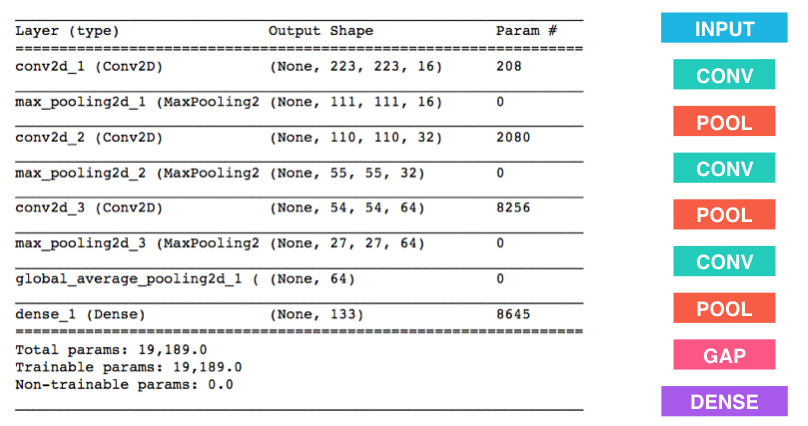
\includegraphics{images/sample_cnn.png}
\caption{Sample CNN}
\end{figure}

\textbf{Question 4:} Outline the steps you took to get to your final CNN
architecture and your reasoning at each step. If you chose to use the
hinted architecture above, describe why you think that CNN architecture
should work well for the image classification task.

\textbf{Answer:}\\
Because the fist convolutional layer detects the edges, the second one
is the collection of edges, and the third one will detect more complex
objects, and maybe there are such a big difference between the breeds,
as the third layer can detect them correctly.

    \begin{Verbatim}[commandchars=\\\{\}]
{\color{incolor}In [{\color{incolor}13}]:} \PY{k+kn}{from} \PY{n+nn}{keras}\PY{n+nn}{.}\PY{n+nn}{layers} \PY{k}{import} \PY{n}{Conv2D}\PY{p}{,} \PY{n}{MaxPooling2D}\PY{p}{,} \PY{n}{GlobalAveragePooling2D}
         \PY{k+kn}{from} \PY{n+nn}{keras}\PY{n+nn}{.}\PY{n+nn}{layers} \PY{k}{import} \PY{n}{Dropout}\PY{p}{,} \PY{n}{Flatten}\PY{p}{,} \PY{n}{Dense}
         \PY{k+kn}{from} \PY{n+nn}{keras}\PY{n+nn}{.}\PY{n+nn}{models} \PY{k}{import} \PY{n}{Sequential}
         
         \PY{n}{model} \PY{o}{=} \PY{n}{Sequential}\PY{p}{(}\PY{p}{)}
         
         \PY{c+c1}{\PYZsh{}\PYZsh{}\PYZsh{} TODO: Define your architecture.}
         \PY{n}{model}\PY{o}{.}\PY{n}{add}\PY{p}{(}\PY{n}{Conv2D}\PY{p}{(}\PY{n}{filters}\PY{o}{=}\PY{l+m+mi}{16}\PY{p}{,} \PY{n}{kernel\PYZus{}size}\PY{o}{=}\PY{l+m+mi}{2}\PY{p}{,} \PY{n}{padding}\PY{o}{=}\PY{l+s+s1}{\PYZsq{}}\PY{l+s+s1}{valid}\PY{l+s+s1}{\PYZsq{}}\PY{p}{,} \PY{n}{activation}\PY{o}{=}\PY{l+s+s1}{\PYZsq{}}\PY{l+s+s1}{relu}\PY{l+s+s1}{\PYZsq{}}\PY{p}{,} 
                                 \PY{n}{input\PYZus{}shape}\PY{o}{=}\PY{p}{(}\PY{l+m+mi}{224}\PY{p}{,} \PY{l+m+mi}{224}\PY{p}{,} \PY{l+m+mi}{3}\PY{p}{)}\PY{p}{)}\PY{p}{)}
         \PY{n}{model}\PY{o}{.}\PY{n}{add}\PY{p}{(}\PY{n}{MaxPooling2D}\PY{p}{(}\PY{n}{pool\PYZus{}size}\PY{o}{=}\PY{l+m+mi}{2}\PY{p}{)}\PY{p}{)}
         \PY{n}{model}\PY{o}{.}\PY{n}{add}\PY{p}{(}\PY{n}{Conv2D}\PY{p}{(}\PY{n}{filters}\PY{o}{=}\PY{l+m+mi}{32}\PY{p}{,} \PY{n}{kernel\PYZus{}size}\PY{o}{=}\PY{l+m+mi}{2}\PY{p}{,} \PY{n}{padding}\PY{o}{=}\PY{l+s+s1}{\PYZsq{}}\PY{l+s+s1}{valid}\PY{l+s+s1}{\PYZsq{}}\PY{p}{,} \PY{n}{activation}\PY{o}{=}\PY{l+s+s1}{\PYZsq{}}\PY{l+s+s1}{relu}\PY{l+s+s1}{\PYZsq{}}\PY{p}{)}\PY{p}{)}
         \PY{n}{model}\PY{o}{.}\PY{n}{add}\PY{p}{(}\PY{n}{MaxPooling2D}\PY{p}{(}\PY{n}{pool\PYZus{}size}\PY{o}{=}\PY{l+m+mi}{2}\PY{p}{)}\PY{p}{)}
         \PY{n}{model}\PY{o}{.}\PY{n}{add}\PY{p}{(}\PY{n}{Conv2D}\PY{p}{(}\PY{n}{filters}\PY{o}{=}\PY{l+m+mi}{64}\PY{p}{,} \PY{n}{kernel\PYZus{}size}\PY{o}{=}\PY{l+m+mi}{2}\PY{p}{,} \PY{n}{padding}\PY{o}{=}\PY{l+s+s1}{\PYZsq{}}\PY{l+s+s1}{valid}\PY{l+s+s1}{\PYZsq{}}\PY{p}{,} \PY{n}{activation}\PY{o}{=}\PY{l+s+s1}{\PYZsq{}}\PY{l+s+s1}{relu}\PY{l+s+s1}{\PYZsq{}}\PY{p}{)}\PY{p}{)}
         \PY{n}{model}\PY{o}{.}\PY{n}{add}\PY{p}{(}\PY{n}{MaxPooling2D}\PY{p}{(}\PY{n}{pool\PYZus{}size}\PY{o}{=}\PY{l+m+mi}{2}\PY{p}{)}\PY{p}{)}
         \PY{n}{model}\PY{o}{.}\PY{n}{add}\PY{p}{(}\PY{n}{GlobalAveragePooling2D}\PY{p}{(}\PY{p}{)}\PY{p}{)}
         \PY{c+c1}{\PYZsh{}model.add(Flatten())}
         \PY{n}{model}\PY{o}{.}\PY{n}{add}\PY{p}{(}\PY{n}{Dense}\PY{p}{(}\PY{l+m+mi}{133}\PY{p}{,} \PY{n}{activation}\PY{o}{=}\PY{l+s+s2}{\PYZdq{}}\PY{l+s+s2}{softmax}\PY{l+s+s2}{\PYZdq{}}\PY{p}{)}\PY{p}{)}
         \PY{n}{model}\PY{o}{.}\PY{n}{summary}\PY{p}{(}\PY{p}{)}
\end{Verbatim}


    \begin{Verbatim}[commandchars=\\\{\}]
\_\_\_\_\_\_\_\_\_\_\_\_\_\_\_\_\_\_\_\_\_\_\_\_\_\_\_\_\_\_\_\_\_\_\_\_\_\_\_\_\_\_\_\_\_\_\_\_\_\_\_\_\_\_\_\_\_\_\_\_\_\_\_\_\_
Layer (type)                 Output Shape              Param \#   
=================================================================
conv2d\_1 (Conv2D)            (None, 223, 223, 16)      208       
\_\_\_\_\_\_\_\_\_\_\_\_\_\_\_\_\_\_\_\_\_\_\_\_\_\_\_\_\_\_\_\_\_\_\_\_\_\_\_\_\_\_\_\_\_\_\_\_\_\_\_\_\_\_\_\_\_\_\_\_\_\_\_\_\_
max\_pooling2d\_2 (MaxPooling2 (None, 111, 111, 16)      0         
\_\_\_\_\_\_\_\_\_\_\_\_\_\_\_\_\_\_\_\_\_\_\_\_\_\_\_\_\_\_\_\_\_\_\_\_\_\_\_\_\_\_\_\_\_\_\_\_\_\_\_\_\_\_\_\_\_\_\_\_\_\_\_\_\_
conv2d\_2 (Conv2D)            (None, 110, 110, 32)      2080      
\_\_\_\_\_\_\_\_\_\_\_\_\_\_\_\_\_\_\_\_\_\_\_\_\_\_\_\_\_\_\_\_\_\_\_\_\_\_\_\_\_\_\_\_\_\_\_\_\_\_\_\_\_\_\_\_\_\_\_\_\_\_\_\_\_
max\_pooling2d\_3 (MaxPooling2 (None, 55, 55, 32)        0         
\_\_\_\_\_\_\_\_\_\_\_\_\_\_\_\_\_\_\_\_\_\_\_\_\_\_\_\_\_\_\_\_\_\_\_\_\_\_\_\_\_\_\_\_\_\_\_\_\_\_\_\_\_\_\_\_\_\_\_\_\_\_\_\_\_
conv2d\_3 (Conv2D)            (None, 54, 54, 64)        8256      
\_\_\_\_\_\_\_\_\_\_\_\_\_\_\_\_\_\_\_\_\_\_\_\_\_\_\_\_\_\_\_\_\_\_\_\_\_\_\_\_\_\_\_\_\_\_\_\_\_\_\_\_\_\_\_\_\_\_\_\_\_\_\_\_\_
max\_pooling2d\_4 (MaxPooling2 (None, 27, 27, 64)        0         
\_\_\_\_\_\_\_\_\_\_\_\_\_\_\_\_\_\_\_\_\_\_\_\_\_\_\_\_\_\_\_\_\_\_\_\_\_\_\_\_\_\_\_\_\_\_\_\_\_\_\_\_\_\_\_\_\_\_\_\_\_\_\_\_\_
global\_average\_pooling2d\_1 ( (None, 64)                0         
\_\_\_\_\_\_\_\_\_\_\_\_\_\_\_\_\_\_\_\_\_\_\_\_\_\_\_\_\_\_\_\_\_\_\_\_\_\_\_\_\_\_\_\_\_\_\_\_\_\_\_\_\_\_\_\_\_\_\_\_\_\_\_\_\_
dense\_1 (Dense)              (None, 133)               8645      
=================================================================
Total params: 19,189
Trainable params: 19,189
Non-trainable params: 0
\_\_\_\_\_\_\_\_\_\_\_\_\_\_\_\_\_\_\_\_\_\_\_\_\_\_\_\_\_\_\_\_\_\_\_\_\_\_\_\_\_\_\_\_\_\_\_\_\_\_\_\_\_\_\_\_\_\_\_\_\_\_\_\_\_

    \end{Verbatim}

    \subsubsection{Compile the Model}\label{compile-the-model}

    \begin{Verbatim}[commandchars=\\\{\}]
{\color{incolor}In [{\color{incolor}14}]:} \PY{n}{model}\PY{o}{.}\PY{n}{compile}\PY{p}{(}\PY{n}{optimizer}\PY{o}{=}\PY{l+s+s1}{\PYZsq{}}\PY{l+s+s1}{rmsprop}\PY{l+s+s1}{\PYZsq{}}\PY{p}{,} \PY{n}{loss}\PY{o}{=}\PY{l+s+s1}{\PYZsq{}}\PY{l+s+s1}{categorical\PYZus{}crossentropy}\PY{l+s+s1}{\PYZsq{}}\PY{p}{,} \PY{n}{metrics}\PY{o}{=}\PY{p}{[}\PY{l+s+s1}{\PYZsq{}}\PY{l+s+s1}{accuracy}\PY{l+s+s1}{\PYZsq{}}\PY{p}{]}\PY{p}{)}
\end{Verbatim}


    \subsubsection{(IMPLEMENTATION) Train the
Model}\label{implementation-train-the-model}

Train your model in the code cell below. Use model checkpointing to save
the model that attains the best validation loss.

You are welcome to
\href{https://blog.keras.io/building-powerful-image-classification-models-using-very-little-data.html}{augment
the training data}, but this is not a requirement.

    \begin{Verbatim}[commandchars=\\\{\}]
{\color{incolor}In [{\color{incolor}15}]:} \PY{k+kn}{from} \PY{n+nn}{keras}\PY{n+nn}{.}\PY{n+nn}{callbacks} \PY{k}{import} \PY{n}{ModelCheckpoint}  
         
         \PY{c+c1}{\PYZsh{}\PYZsh{}\PYZsh{} TODO: specify the number of epochs that you would like to use to train the model.}
         
         \PY{n}{epochs} \PY{o}{=} \PY{l+m+mi}{5}
         
         \PY{c+c1}{\PYZsh{}\PYZsh{}\PYZsh{} Do NOT modify the code below this line.}
         
         \PY{n}{checkpointer} \PY{o}{=} \PY{n}{ModelCheckpoint}\PY{p}{(}\PY{n}{filepath}\PY{o}{=}\PY{l+s+s1}{\PYZsq{}}\PY{l+s+s1}{saved\PYZus{}models/weights.best.from\PYZus{}scratch.hdf5}\PY{l+s+s1}{\PYZsq{}}\PY{p}{,} 
                                        \PY{n}{verbose}\PY{o}{=}\PY{l+m+mi}{1}\PY{p}{,} \PY{n}{save\PYZus{}best\PYZus{}only}\PY{o}{=}\PY{k+kc}{True}\PY{p}{)}
         
         \PY{n}{model}\PY{o}{.}\PY{n}{fit}\PY{p}{(}\PY{n}{train\PYZus{}tensors}\PY{p}{,} \PY{n}{train\PYZus{}targets}\PY{p}{,} 
                   \PY{n}{validation\PYZus{}data}\PY{o}{=}\PY{p}{(}\PY{n}{valid\PYZus{}tensors}\PY{p}{,} \PY{n}{valid\PYZus{}targets}\PY{p}{)}\PY{p}{,}
                   \PY{n}{epochs}\PY{o}{=}\PY{n}{epochs}\PY{p}{,} \PY{n}{batch\PYZus{}size}\PY{o}{=}\PY{l+m+mi}{20}\PY{p}{,} \PY{n}{callbacks}\PY{o}{=}\PY{p}{[}\PY{n}{checkpointer}\PY{p}{]}\PY{p}{,} \PY{n}{verbose}\PY{o}{=}\PY{l+m+mi}{1}\PY{p}{)}
\end{Verbatim}


    \begin{Verbatim}[commandchars=\\\{\}]
Train on 6680 samples, validate on 835 samples
Epoch 1/5
4040/6680 [=================>{\ldots}] - ETA: 659s - loss: 4.9202 - acc: 0.0000e+0 - ETA: 411s - loss: 4.9143 - acc: 0.0000e+0 - ETA: 326s - loss: 4.9223 - acc: 0.0000e+0 - ETA: 301s - loss: 4.9150 - acc: 0.0000e+0 - ETA: 308s - loss: 4.9126 - acc: 0.0000e+0 - ETA: 313s - loss: 4.9083 - acc: 0.0000e+0 - ETA: 317s - loss: 4.9074 - acc: 0.0000e+0 - ETA: 319s - loss: 4.9050 - acc: 0.0000e+0 - ETA: 325s - loss: 4.8997 - acc: 0.0056    - ETA: 328s - loss: 4.8988 - acc: 0.005 - ETA: 330s - loss: 4.8964 - acc: 0.009 - ETA: 330s - loss: 4.8970 - acc: 0.008 - ETA: 331s - loss: 4.8956 - acc: 0.007 - ETA: 330s - loss: 4.8965 - acc: 0.007 - ETA: 330s - loss: 4.8968 - acc: 0.006 - ETA: 329s - loss: 4.8961 - acc: 0.006 - ETA: 328s - loss: 4.8945 - acc: 0.005 - ETA: 327s - loss: 4.8931 - acc: 0.005 - ETA: 326s - loss: 4.8926 - acc: 0.005 - ETA: 326s - loss: 4.8932 - acc: 0.005 - ETA: 325s - loss: 4.8944 - acc: 0.004 - ETA: 324s - loss: 4.8959 - acc: 0.004 - ETA: 323s - loss: 4.8972 - acc: 0.004 - ETA: 321s - loss: 4.8967 - acc: 0.004 - ETA: 320s - loss: 4.8962 - acc: 0.004 - ETA: 319s - loss: 4.8958 - acc: 0.003 - ETA: 318s - loss: 4.8949 - acc: 0.003 - ETA: 317s - loss: 4.8926 - acc: 0.005 - ETA: 316s - loss: 4.8935 - acc: 0.005 - ETA: 315s - loss: 4.8930 - acc: 0.005 - ETA: 314s - loss: 4.8934 - acc: 0.004 - ETA: 313s - loss: 4.8941 - acc: 0.004 - ETA: 312s - loss: 4.8927 - acc: 0.004 - ETA: 311s - loss: 4.8920 - acc: 0.004 - ETA: 310s - loss: 4.8911 - acc: 0.004 - ETA: 309s - loss: 4.8909 - acc: 0.004 - ETA: 308s - loss: 4.8894 - acc: 0.004 - ETA: 307s - loss: 4.8882 - acc: 0.003 - ETA: 306s - loss: 4.8883 - acc: 0.003 - ETA: 305s - loss: 4.8885 - acc: 0.003 - ETA: 304s - loss: 4.8884 - acc: 0.004 - ETA: 303s - loss: 4.8882 - acc: 0.004 - ETA: 302s - loss: 4.8880 - acc: 0.004 - ETA: 301s - loss: 4.8861 - acc: 0.004 - ETA: 300s - loss: 4.8875 - acc: 0.004 - ETA: 299s - loss: 4.8871 - acc: 0.004 - ETA: 298s - loss: 4.8881 - acc: 0.004 - ETA: 297s - loss: 4.8884 - acc: 0.004 - ETA: 296s - loss: 4.8886 - acc: 0.004 - ETA: 295s - loss: 4.8888 - acc: 0.005 - ETA: 294s - loss: 4.8895 - acc: 0.004 - ETA: 293s - loss: 4.8896 - acc: 0.004 - ETA: 292s - loss: 4.8906 - acc: 0.004 - ETA: 291s - loss: 4.8906 - acc: 0.004 - ETA: 291s - loss: 4.8900 - acc: 0.004 - ETA: 290s - loss: 4.8895 - acc: 0.004 - ETA: 289s - loss: 4.8891 - acc: 0.004 - ETA: 288s - loss: 4.8883 - acc: 0.004 - ETA: 286s - loss: 4.8897 - acc: 0.004 - ETA: 286s - loss: 4.8902 - acc: 0.004 - ETA: 284s - loss: 4.8908 - acc: 0.004 - ETA: 283s - loss: 4.8909 - acc: 0.004 - ETA: 282s - loss: 4.8909 - acc: 0.004 - ETA: 281s - loss: 4.8913 - acc: 0.003 - ETA: 280s - loss: 4.8913 - acc: 0.003 - ETA: 279s - loss: 4.8915 - acc: 0.003 - ETA: 278s - loss: 4.8910 - acc: 0.003 - ETA: 277s - loss: 4.8910 - acc: 0.003 - ETA: 276s - loss: 4.8907 - acc: 0.003 - ETA: 275s - loss: 4.8905 - acc: 0.003 - ETA: 274s - loss: 4.8904 - acc: 0.003 - ETA: 273s - loss: 4.8901 - acc: 0.003 - ETA: 272s - loss: 4.8901 - acc: 0.003 - ETA: 271s - loss: 4.8905 - acc: 0.003 - ETA: 270s - loss: 4.8905 - acc: 0.003 - ETA: 269s - loss: 4.8900 - acc: 0.003 - ETA: 268s - loss: 4.8897 - acc: 0.003 - ETA: 267s - loss: 4.8901 - acc: 0.003 - ETA: 266s - loss: 4.8902 - acc: 0.003 - ETA: 265s - loss: 4.8904 - acc: 0.003 - ETA: 263s - loss: 4.8902 - acc: 0.003 - ETA: 262s - loss: 4.8899 - acc: 0.003 - ETA: 261s - loss: 4.8897 - acc: 0.003 - ETA: 260s - loss: 4.8895 - acc: 0.003 - ETA: 259s - loss: 4.8893 - acc: 0.003 - ETA: 258s - loss: 4.8891 - acc: 0.003 - ETA: 257s - loss: 4.8891 - acc: 0.003 - ETA: 256s - loss: 4.8893 - acc: 0.003 - ETA: 255s - loss: 4.8895 - acc: 0.003 - ETA: 254s - loss: 4.8892 - acc: 0.003 - ETA: 253s - loss: 4.8892 - acc: 0.003 - ETA: 252s - loss: 4.8888 - acc: 0.003 - ETA: 251s - loss: 4.8889 - acc: 0.004 - ETA: 250s - loss: 4.8890 - acc: 0.004 - ETA: 249s - loss: 4.8892 - acc: 0.004 - ETA: 248s - loss: 4.8888 - acc: 0.004 - ETA: 247s - loss: 4.8888 - acc: 0.004 - ETA: 246s - loss: 4.8885 - acc: 0.004 - ETA: 246s - loss: 4.8885 - acc: 0.005 - ETA: 245s - loss: 4.8889 - acc: 0.005 - ETA: 245s - loss: 4.8889 - acc: 0.005 - ETA: 244s - loss: 4.8889 - acc: 0.005 - ETA: 243s - loss: 4.8884 - acc: 0.005 - ETA: 241s - loss: 4.8881 - acc: 0.005 - ETA: 240s - loss: 4.8879 - acc: 0.005 - ETA: 239s - loss: 4.8881 - acc: 0.005 - ETA: 239s - loss: 4.8883 - acc: 0.005 - ETA: 238s - loss: 4.8883 - acc: 0.006 - ETA: 236s - loss: 4.8885 - acc: 0.006 - ETA: 235s - loss: 4.8884 - acc: 0.005 - ETA: 234s - loss: 4.8885 - acc: 0.005 - ETA: 233s - loss: 4.8883 - acc: 0.005 - ETA: 232s - loss: 4.8880 - acc: 0.006 - ETA: 231s - loss: 4.8880 - acc: 0.006 - ETA: 230s - loss: 4.8881 - acc: 0.006 - ETA: 229s - loss: 4.8880 - acc: 0.006 - ETA: 228s - loss: 4.8879 - acc: 0.006 - ETA: 227s - loss: 4.8879 - acc: 0.005 - ETA: 226s - loss: 4.8877 - acc: 0.005 - ETA: 225s - loss: 4.8873 - acc: 0.005 - ETA: 225s - loss: 4.8873 - acc: 0.005 - ETA: 223s - loss: 4.8871 - acc: 0.005 - ETA: 223s - loss: 4.8872 - acc: 0.006 - ETA: 222s - loss: 4.8872 - acc: 0.006 - ETA: 221s - loss: 4.8871 - acc: 0.006 - ETA: 220s - loss: 4.8873 - acc: 0.006 - ETA: 219s - loss: 4.8871 - acc: 0.006 - ETA: 218s - loss: 4.8873 - acc: 0.007 - ETA: 217s - loss: 4.8871 - acc: 0.007 - ETA: 216s - loss: 4.8869 - acc: 0.006 - ETA: 215s - loss: 4.8872 - acc: 0.006 - ETA: 214s - loss: 4.8865 - acc: 0.006 - ETA: 213s - loss: 4.8861 - acc: 0.006 - ETA: 212s - loss: 4.8857 - acc: 0.006 - ETA: 210s - loss: 4.8860 - acc: 0.006 - ETA: 209s - loss: 4.8864 - acc: 0.006 - ETA: 209s - loss: 4.8861 - acc: 0.006 - ETA: 208s - loss: 4.8863 - acc: 0.006 - ETA: 207s - loss: 4.8860 - acc: 0.006 - ETA: 206s - loss: 4.8863 - acc: 0.006 - ETA: 205s - loss: 4.8862 - acc: 0.006 - ETA: 204s - loss: 4.8864 - acc: 0.006 - ETA: 203s - loss: 4.8870 - acc: 0.006 - ETA: 202s - loss: 4.8865 - acc: 0.006 - ETA: 201s - loss: 4.8867 - acc: 0.006 - ETA: 201s - loss: 4.8869 - acc: 0.006 - ETA: 200s - loss: 4.8866 - acc: 0.007 - ETA: 199s - loss: 4.8868 - acc: 0.007 - ETA: 198s - loss: 4.8870 - acc: 0.007 - ETA: 197s - loss: 4.8871 - acc: 0.007 - ETA: 196s - loss: 4.8873 - acc: 0.007 - ETA: 195s - loss: 4.8872 - acc: 0.007 - ETA: 194s - loss: 4.8874 - acc: 0.007 - ETA: 193s - loss: 4.8875 - acc: 0.007 - ETA: 192s - loss: 4.8873 - acc: 0.007 - ETA: 191s - loss: 4.8873 - acc: 0.007 - ETA: 190s - loss: 4.8873 - acc: 0.007 - ETA: 189s - loss: 4.8873 - acc: 0.007 - ETA: 188s - loss: 4.8870 - acc: 0.007 - ETA: 187s - loss: 4.8870 - acc: 0.007 - ETA: 186s - loss: 4.8868 - acc: 0.007 - ETA: 184s - loss: 4.8868 - acc: 0.007 - ETA: 183s - loss: 4.8868 - acc: 0.007 - ETA: 182s - loss: 4.8867 - acc: 0.007 - ETA: 181s - loss: 4.8866 - acc: 0.007 - ETA: 180s - loss: 4.8868 - acc: 0.007 - ETA: 179s - loss: 4.8871 - acc: 0.007 - ETA: 178s - loss: 4.8873 - acc: 0.008 - ETA: 177s - loss: 4.8874 - acc: 0.008 - ETA: 175s - loss: 4.8875 - acc: 0.007 - ETA: 174s - loss: 4.8875 - acc: 0.007 - ETA: 173s - loss: 4.8874 - acc: 0.008 - ETA: 172s - loss: 4.8872 - acc: 0.008 - ETA: 171s - loss: 4.8870 - acc: 0.008 - ETA: 170s - loss: 4.8872 - acc: 0.008 - ETA: 169s - loss: 4.8872 - acc: 0.008 - ETA: 168s - loss: 4.8871 - acc: 0.008 - ETA: 167s - loss: 4.8871 - acc: 0.008 - ETA: 166s - loss: 4.8869 - acc: 0.008 - ETA: 165s - loss: 4.8870 - acc: 0.008 - ETA: 164s - loss: 4.8871 - acc: 0.008 - ETA: 163s - loss: 4.8871 - acc: 0.008 - ETA: 162s - loss: 4.8869 - acc: 0.008 - ETA: 161s - loss: 4.8869 - acc: 0.008 - ETA: 160s - loss: 4.8869 - acc: 0.008 - ETA: 159s - loss: 4.8870 - acc: 0.008 - ETA: 158s - loss: 4.8868 - acc: 0.008 - ETA: 157s - loss: 4.8868 - acc: 0.008 - ETA: 156s - loss: 4.8867 - acc: 0.007 - ETA: 155s - loss: 4.8864 - acc: 0.007 - ETA: 154s - loss: 4.8864 - acc: 0.007 - ETA: 153s - loss: 4.8864 - acc: 0.007 - ETA: 152s - loss: 4.8862 - acc: 0.007 - ETA: 151s - loss: 4.8859 - acc: 0.008 - ETA: 150s - loss: 4.8858 - acc: 0.007 - ETA: 149s - loss: 4.8858 - acc: 0.007 - ETA: 148s - loss: 4.8856 - acc: 0.007 - ETA: 147s - loss: 4.8858 - acc: 0.007 - ETA: 146s - loss: 4.8858 - acc: 0.007 - ETA: 144s - loss: 4.8860 - acc: 0.007 - ETA: 143s - loss: 4.8860 - acc: 0.007 - ETA: 142s - loss: 4.8859 - acc: 0.00796660/6680 [============================>.] - ETA: 141s - loss: 4.8859 - acc: 0.007 - ETA: 140s - loss: 4.8858 - acc: 0.007 - ETA: 139s - loss: 4.8859 - acc: 0.007 - ETA: 138s - loss: 4.8860 - acc: 0.007 - ETA: 137s - loss: 4.8857 - acc: 0.008 - ETA: 136s - loss: 4.8854 - acc: 0.007 - ETA: 135s - loss: 4.8856 - acc: 0.007 - ETA: 134s - loss: 4.8853 - acc: 0.007 - ETA: 132s - loss: 4.8854 - acc: 0.007 - ETA: 131s - loss: 4.8851 - acc: 0.008 - ETA: 130s - loss: 4.8851 - acc: 0.008 - ETA: 129s - loss: 4.8849 - acc: 0.007 - ETA: 128s - loss: 4.8847 - acc: 0.008 - ETA: 127s - loss: 4.8847 - acc: 0.008 - ETA: 126s - loss: 4.8847 - acc: 0.008 - ETA: 125s - loss: 4.8847 - acc: 0.008 - ETA: 124s - loss: 4.8845 - acc: 0.008 - ETA: 123s - loss: 4.8844 - acc: 0.008 - ETA: 122s - loss: 4.8847 - acc: 0.008 - ETA: 121s - loss: 4.8849 - acc: 0.008 - ETA: 120s - loss: 4.8850 - acc: 0.008 - ETA: 118s - loss: 4.8849 - acc: 0.008 - ETA: 117s - loss: 4.8851 - acc: 0.008 - ETA: 116s - loss: 4.8850 - acc: 0.008 - ETA: 115s - loss: 4.8849 - acc: 0.007 - ETA: 114s - loss: 4.8846 - acc: 0.008 - ETA: 113s - loss: 4.8847 - acc: 0.008 - ETA: 112s - loss: 4.8848 - acc: 0.008 - ETA: 111s - loss: 4.8847 - acc: 0.008 - ETA: 110s - loss: 4.8847 - acc: 0.008 - ETA: 109s - loss: 4.8848 - acc: 0.008 - ETA: 108s - loss: 4.8850 - acc: 0.008 - ETA: 107s - loss: 4.8849 - acc: 0.008 - ETA: 105s - loss: 4.8850 - acc: 0.008 - ETA: 104s - loss: 4.8851 - acc: 0.008 - ETA: 103s - loss: 4.8849 - acc: 0.008 - ETA: 102s - loss: 4.8849 - acc: 0.008 - ETA: 102s - loss: 4.8847 - acc: 0.008 - ETA: 101s - loss: 4.8848 - acc: 0.008 - ETA: 100s - loss: 4.8846 - acc: 0.008 - ETA: 99s - loss: 4.8844 - acc: 0.008 - ETA: 98s - loss: 4.8843 - acc: 0.00 - ETA: 97s - loss: 4.8844 - acc: 0.00 - ETA: 96s - loss: 4.8844 - acc: 0.00 - ETA: 95s - loss: 4.8845 - acc: 0.00 - ETA: 94s - loss: 4.8845 - acc: 0.00 - ETA: 92s - loss: 4.8848 - acc: 0.00 - ETA: 91s - loss: 4.8847 - acc: 0.00 - ETA: 90s - loss: 4.8847 - acc: 0.00 - ETA: 89s - loss: 4.8847 - acc: 0.00 - ETA: 88s - loss: 4.8847 - acc: 0.00 - ETA: 87s - loss: 4.8847 - acc: 0.00 - ETA: 86s - loss: 4.8847 - acc: 0.00 - ETA: 85s - loss: 4.8844 - acc: 0.00 - ETA: 84s - loss: 4.8846 - acc: 0.00 - ETA: 83s - loss: 4.8845 - acc: 0.00 - ETA: 81s - loss: 4.8845 - acc: 0.00 - ETA: 80s - loss: 4.8846 - acc: 0.00 - ETA: 79s - loss: 4.8847 - acc: 0.00 - ETA: 78s - loss: 4.8846 - acc: 0.00 - ETA: 77s - loss: 4.8847 - acc: 0.00 - ETA: 76s - loss: 4.8846 - acc: 0.00 - ETA: 75s - loss: 4.8847 - acc: 0.00 - ETA: 74s - loss: 4.8848 - acc: 0.00 - ETA: 73s - loss: 4.8846 - acc: 0.00 - ETA: 72s - loss: 4.8847 - acc: 0.00 - ETA: 71s - loss: 4.8848 - acc: 0.00 - ETA: 69s - loss: 4.8849 - acc: 0.00 - ETA: 68s - loss: 4.8851 - acc: 0.00 - ETA: 67s - loss: 4.8850 - acc: 0.00 - ETA: 66s - loss: 4.8851 - acc: 0.00 - ETA: 65s - loss: 4.8851 - acc: 0.00 - ETA: 64s - loss: 4.8851 - acc: 0.00 - ETA: 63s - loss: 4.8850 - acc: 0.00 - ETA: 62s - loss: 4.8850 - acc: 0.00 - ETA: 61s - loss: 4.8849 - acc: 0.00 - ETA: 60s - loss: 4.8847 - acc: 0.00 - ETA: 58s - loss: 4.8845 - acc: 0.00 - ETA: 57s - loss: 4.8844 - acc: 0.00 - ETA: 56s - loss: 4.8843 - acc: 0.00 - ETA: 55s - loss: 4.8845 - acc: 0.00 - ETA: 54s - loss: 4.8844 - acc: 0.00 - ETA: 53s - loss: 4.8845 - acc: 0.00 - ETA: 52s - loss: 4.8846 - acc: 0.00 - ETA: 51s - loss: 4.8846 - acc: 0.00 - ETA: 50s - loss: 4.8846 - acc: 0.00 - ETA: 49s - loss: 4.8845 - acc: 0.00 - ETA: 47s - loss: 4.8845 - acc: 0.00 - ETA: 46s - loss: 4.8845 - acc: 0.00 - ETA: 45s - loss: 4.8846 - acc: 0.00 - ETA: 44s - loss: 4.8847 - acc: 0.00 - ETA: 43s - loss: 4.8846 - acc: 0.00 - ETA: 42s - loss: 4.8847 - acc: 0.00 - ETA: 41s - loss: 4.8848 - acc: 0.00 - ETA: 40s - loss: 4.8848 - acc: 0.00 - ETA: 39s - loss: 4.8847 - acc: 0.00 - ETA: 38s - loss: 4.8847 - acc: 0.00 - ETA: 36s - loss: 4.8848 - acc: 0.00 - ETA: 35s - loss: 4.8847 - acc: 0.00 - ETA: 34s - loss: 4.8846 - acc: 0.00 - ETA: 33s - loss: 4.8845 - acc: 0.00 - ETA: 32s - loss: 4.8844 - acc: 0.00 - ETA: 31s - loss: 4.8843 - acc: 0.00 - ETA: 30s - loss: 4.8844 - acc: 0.00 - ETA: 29s - loss: 4.8843 - acc: 0.00 - ETA: 28s - loss: 4.8843 - acc: 0.00 - ETA: 27s - loss: 4.8843 - acc: 0.00 - ETA: 26s - loss: 4.8842 - acc: 0.00 - ETA: 24s - loss: 4.8842 - acc: 0.00 - ETA: 23s - loss: 4.8841 - acc: 0.00 - ETA: 22s - loss: 4.8838 - acc: 0.00 - ETA: 21s - loss: 4.8839 - acc: 0.00 - ETA: 20s - loss: 4.8842 - acc: 0.00 - ETA: 19s - loss: 4.8841 - acc: 0.00 - ETA: 18s - loss: 4.8841 - acc: 0.00 - ETA: 17s - loss: 4.8840 - acc: 0.00 - ETA: 16s - loss: 4.8840 - acc: 0.00 - ETA: 15s - loss: 4.8839 - acc: 0.00 - ETA: 14s - loss: 4.8842 - acc: 0.00 - ETA: 13s - loss: 4.8843 - acc: 0.00 - ETA: 11s - loss: 4.8842 - acc: 0.00 - ETA: 10s - loss: 4.8843 - acc: 0.00 - ETA: 9s - loss: 4.8842 - acc: 0.0091 - ETA: 8s - loss: 4.8841 - acc: 0.009 - ETA: 7s - loss: 4.8839 - acc: 0.009 - ETA: 6s - loss: 4.8837 - acc: 0.009 - ETA: 5s - loss: 4.8839 - acc: 0.009 - ETA: 4s - loss: 4.8839 - acc: 0.009 - ETA: 3s - loss: 4.8839 - acc: 0.009 - ETA: 2s - loss: 4.8838 - acc: 0.009 - ETA: 1s - loss: 4.8837 - acc: 0.0093Epoch 00000: val\_loss improved from inf to 4.86615, saving model to saved\_models/weights.best.from\_scratch.hdf5
6680/6680 [==============================] - 379s - loss: 4.8838 - acc: 0.0093 - val\_loss: 4.8661 - val\_acc: 0.0132
Epoch 2/5
4080/6680 [=================>{\ldots}] - ETA: 326s - loss: 4.8895 - acc: 0.0000e+0 - ETA: 323s - loss: 4.8803 - acc: 0.0000e+0 - ETA: 323s - loss: 4.8836 - acc: 0.0000e+0 - ETA: 326s - loss: 4.8912 - acc: 0.0000e+0 - ETA: 324s - loss: 4.8828 - acc: 0.0300    - ETA: 323s - loss: 4.8790 - acc: 0.025 - ETA: 322s - loss: 4.8780 - acc: 0.021 - ETA: 322s - loss: 4.8747 - acc: 0.018 - ETA: 322s - loss: 4.8742 - acc: 0.016 - ETA: 322s - loss: 4.8709 - acc: 0.015 - ETA: 324s - loss: 4.8685 - acc: 0.013 - ETA: 329s - loss: 4.8668 - acc: 0.016 - ETA: 330s - loss: 4.8694 - acc: 0.015 - ETA: 334s - loss: 4.8650 - acc: 0.017 - ETA: 335s - loss: 4.8649 - acc: 0.016 - ETA: 336s - loss: 4.8637 - acc: 0.015 - ETA: 335s - loss: 4.8636 - acc: 0.014 - ETA: 334s - loss: 4.8702 - acc: 0.013 - ETA: 333s - loss: 4.8693 - acc: 0.013 - ETA: 330s - loss: 4.8682 - acc: 0.012 - ETA: 328s - loss: 4.8675 - acc: 0.011 - ETA: 326s - loss: 4.8733 - acc: 0.011 - ETA: 325s - loss: 4.8742 - acc: 0.010 - ETA: 324s - loss: 4.8745 - acc: 0.010 - ETA: 323s - loss: 4.8741 - acc: 0.010 - ETA: 322s - loss: 4.8738 - acc: 0.009 - ETA: 321s - loss: 4.8731 - acc: 0.009 - ETA: 320s - loss: 4.8710 - acc: 0.010 - ETA: 318s - loss: 4.8716 - acc: 0.010 - ETA: 316s - loss: 4.8724 - acc: 0.010 - ETA: 315s - loss: 4.8723 - acc: 0.009 - ETA: 314s - loss: 4.8729 - acc: 0.009 - ETA: 313s - loss: 4.8728 - acc: 0.009 - ETA: 311s - loss: 4.8713 - acc: 0.008 - ETA: 310s - loss: 4.8690 - acc: 0.008 - ETA: 308s - loss: 4.8684 - acc: 0.008 - ETA: 307s - loss: 4.8660 - acc: 0.008 - ETA: 305s - loss: 4.8642 - acc: 0.009 - ETA: 304s - loss: 4.8613 - acc: 0.009 - ETA: 303s - loss: 4.8623 - acc: 0.010 - ETA: 302s - loss: 4.8644 - acc: 0.009 - ETA: 300s - loss: 4.8647 - acc: 0.009 - ETA: 299s - loss: 4.8632 - acc: 0.010 - ETA: 297s - loss: 4.8624 - acc: 0.010 - ETA: 296s - loss: 4.8645 - acc: 0.010 - ETA: 295s - loss: 4.8663 - acc: 0.009 - ETA: 293s - loss: 4.8670 - acc: 0.009 - ETA: 292s - loss: 4.8683 - acc: 0.009 - ETA: 290s - loss: 4.8705 - acc: 0.009 - ETA: 289s - loss: 4.8702 - acc: 0.009 - ETA: 288s - loss: 4.8703 - acc: 0.008 - ETA: 286s - loss: 4.8707 - acc: 0.008 - ETA: 285s - loss: 4.8700 - acc: 0.009 - ETA: 284s - loss: 4.8692 - acc: 0.009 - ETA: 283s - loss: 4.8704 - acc: 0.009 - ETA: 281s - loss: 4.8695 - acc: 0.008 - ETA: 280s - loss: 4.8700 - acc: 0.008 - ETA: 279s - loss: 4.8701 - acc: 0.008 - ETA: 278s - loss: 4.8704 - acc: 0.009 - ETA: 277s - loss: 4.8706 - acc: 0.009 - ETA: 275s - loss: 4.8712 - acc: 0.009 - ETA: 274s - loss: 4.8710 - acc: 0.008 - ETA: 273s - loss: 4.8715 - acc: 0.008 - ETA: 272s - loss: 4.8714 - acc: 0.008 - ETA: 271s - loss: 4.8720 - acc: 0.008 - ETA: 270s - loss: 4.8716 - acc: 0.008 - ETA: 268s - loss: 4.8721 - acc: 0.008 - ETA: 267s - loss: 4.8715 - acc: 0.008 - ETA: 266s - loss: 4.8723 - acc: 0.008 - ETA: 265s - loss: 4.8715 - acc: 0.007 - ETA: 264s - loss: 4.8708 - acc: 0.007 - ETA: 263s - loss: 4.8709 - acc: 0.007 - ETA: 262s - loss: 4.8716 - acc: 0.007 - ETA: 261s - loss: 4.8713 - acc: 0.008 - ETA: 260s - loss: 4.8712 - acc: 0.008 - ETA: 259s - loss: 4.8702 - acc: 0.007 - ETA: 258s - loss: 4.8690 - acc: 0.007 - ETA: 257s - loss: 4.8689 - acc: 0.007 - ETA: 256s - loss: 4.8685 - acc: 0.007 - ETA: 255s - loss: 4.8681 - acc: 0.007 - ETA: 254s - loss: 4.8680 - acc: 0.007 - ETA: 252s - loss: 4.8674 - acc: 0.007 - ETA: 251s - loss: 4.8678 - acc: 0.007 - ETA: 250s - loss: 4.8678 - acc: 0.007 - ETA: 249s - loss: 4.8683 - acc: 0.007 - ETA: 248s - loss: 4.8678 - acc: 0.007 - ETA: 247s - loss: 4.8681 - acc: 0.008 - ETA: 246s - loss: 4.8679 - acc: 0.008 - ETA: 245s - loss: 4.8683 - acc: 0.007 - ETA: 244s - loss: 4.8685 - acc: 0.007 - ETA: 243s - loss: 4.8683 - acc: 0.007 - ETA: 242s - loss: 4.8689 - acc: 0.007 - ETA: 241s - loss: 4.8684 - acc: 0.007 - ETA: 240s - loss: 4.8680 - acc: 0.007 - ETA: 239s - loss: 4.8679 - acc: 0.007 - ETA: 238s - loss: 4.8677 - acc: 0.007 - ETA: 236s - loss: 4.8678 - acc: 0.007 - ETA: 235s - loss: 4.8676 - acc: 0.007 - ETA: 234s - loss: 4.8679 - acc: 0.007 - ETA: 233s - loss: 4.8670 - acc: 0.007 - ETA: 232s - loss: 4.8670 - acc: 0.007 - ETA: 231s - loss: 4.8677 - acc: 0.007 - ETA: 230s - loss: 4.8670 - acc: 0.007 - ETA: 229s - loss: 4.8669 - acc: 0.007 - ETA: 228s - loss: 4.8665 - acc: 0.007 - ETA: 227s - loss: 4.8665 - acc: 0.007 - ETA: 226s - loss: 4.8663 - acc: 0.007 - ETA: 225s - loss: 4.8673 - acc: 0.006 - ETA: 224s - loss: 4.8678 - acc: 0.006 - ETA: 223s - loss: 4.8684 - acc: 0.006 - ETA: 222s - loss: 4.8687 - acc: 0.006 - ETA: 221s - loss: 4.8684 - acc: 0.007 - ETA: 220s - loss: 4.8683 - acc: 0.008 - ETA: 218s - loss: 4.8686 - acc: 0.007 - ETA: 217s - loss: 4.8680 - acc: 0.007 - ETA: 216s - loss: 4.8687 - acc: 0.007 - ETA: 215s - loss: 4.8685 - acc: 0.007 - ETA: 214s - loss: 4.8683 - acc: 0.007 - ETA: 213s - loss: 4.8677 - acc: 0.008 - ETA: 212s - loss: 4.8674 - acc: 0.007 - ETA: 211s - loss: 4.8675 - acc: 0.007 - ETA: 210s - loss: 4.8674 - acc: 0.007 - ETA: 209s - loss: 4.8676 - acc: 0.007 - ETA: 208s - loss: 4.8672 - acc: 0.007 - ETA: 207s - loss: 4.8674 - acc: 0.007 - ETA: 206s - loss: 4.8673 - acc: 0.007 - ETA: 205s - loss: 4.8674 - acc: 0.007 - ETA: 204s - loss: 4.8678 - acc: 0.007 - ETA: 203s - loss: 4.8674 - acc: 0.007 - ETA: 202s - loss: 4.8677 - acc: 0.007 - ETA: 201s - loss: 4.8673 - acc: 0.007 - ETA: 200s - loss: 4.8674 - acc: 0.008 - ETA: 199s - loss: 4.8670 - acc: 0.007 - ETA: 198s - loss: 4.8666 - acc: 0.007 - ETA: 197s - loss: 4.8659 - acc: 0.007 - ETA: 196s - loss: 4.8658 - acc: 0.008 - ETA: 195s - loss: 4.8657 - acc: 0.008 - ETA: 194s - loss: 4.8656 - acc: 0.008 - ETA: 193s - loss: 4.8659 - acc: 0.008 - ETA: 192s - loss: 4.8662 - acc: 0.008 - ETA: 192s - loss: 4.8660 - acc: 0.008 - ETA: 191s - loss: 4.8662 - acc: 0.008 - ETA: 190s - loss: 4.8658 - acc: 0.008 - ETA: 189s - loss: 4.8657 - acc: 0.008 - ETA: 188s - loss: 4.8650 - acc: 0.007 - ETA: 187s - loss: 4.8642 - acc: 0.007 - ETA: 186s - loss: 4.8642 - acc: 0.007 - ETA: 185s - loss: 4.8638 - acc: 0.007 - ETA: 184s - loss: 4.8641 - acc: 0.007 - ETA: 183s - loss: 4.8653 - acc: 0.007 - ETA: 182s - loss: 4.8653 - acc: 0.007 - ETA: 182s - loss: 4.8651 - acc: 0.007 - ETA: 181s - loss: 4.8650 - acc: 0.007 - ETA: 180s - loss: 4.8648 - acc: 0.008 - ETA: 179s - loss: 4.8649 - acc: 0.008 - ETA: 178s - loss: 4.8652 - acc: 0.008 - ETA: 177s - loss: 4.8664 - acc: 0.008 - ETA: 176s - loss: 4.8666 - acc: 0.008 - ETA: 175s - loss: 4.8669 - acc: 0.008 - ETA: 174s - loss: 4.8664 - acc: 0.008 - ETA: 173s - loss: 4.8667 - acc: 0.008 - ETA: 172s - loss: 4.8669 - acc: 0.008 - ETA: 171s - loss: 4.8665 - acc: 0.008 - ETA: 170s - loss: 4.8661 - acc: 0.008 - ETA: 169s - loss: 4.8659 - acc: 0.008 - ETA: 168s - loss: 4.8654 - acc: 0.008 - ETA: 167s - loss: 4.8646 - acc: 0.009 - ETA: 166s - loss: 4.8648 - acc: 0.009 - ETA: 166s - loss: 4.8642 - acc: 0.009 - ETA: 165s - loss: 4.8645 - acc: 0.009 - ETA: 164s - loss: 4.8651 - acc: 0.009 - ETA: 163s - loss: 4.8650 - acc: 0.009 - ETA: 162s - loss: 4.8646 - acc: 0.009 - ETA: 161s - loss: 4.8649 - acc: 0.009 - ETA: 160s - loss: 4.8655 - acc: 0.009 - ETA: 159s - loss: 4.8654 - acc: 0.009 - ETA: 158s - loss: 4.8655 - acc: 0.009 - ETA: 157s - loss: 4.8656 - acc: 0.009 - ETA: 156s - loss: 4.8658 - acc: 0.009 - ETA: 155s - loss: 4.8656 - acc: 0.010 - ETA: 154s - loss: 4.8657 - acc: 0.010 - ETA: 153s - loss: 4.8654 - acc: 0.010 - ETA: 152s - loss: 4.8656 - acc: 0.010 - ETA: 152s - loss: 4.8658 - acc: 0.010 - ETA: 151s - loss: 4.8659 - acc: 0.010 - ETA: 150s - loss: 4.8657 - acc: 0.010 - ETA: 149s - loss: 4.8660 - acc: 0.010 - ETA: 148s - loss: 4.8661 - acc: 0.010 - ETA: 147s - loss: 4.8659 - acc: 0.010 - ETA: 146s - loss: 4.8658 - acc: 0.010 - ETA: 145s - loss: 4.8659 - acc: 0.010 - ETA: 144s - loss: 4.8658 - acc: 0.010 - ETA: 143s - loss: 4.8660 - acc: 0.010 - ETA: 142s - loss: 4.8659 - acc: 0.010 - ETA: 141s - loss: 4.8658 - acc: 0.010 - ETA: 140s - loss: 4.8656 - acc: 0.010 - ETA: 139s - loss: 4.8657 - acc: 0.010 - ETA: 138s - loss: 4.8654 - acc: 0.010 - ETA: 138s - loss: 4.8655 - acc: 0.010 - ETA: 137s - loss: 4.8655 - acc: 0.010 - ETA: 136s - loss: 4.8655 - acc: 0.010 - ETA: 135s - loss: 4.8658 - acc: 0.010 - ETA: 134s - loss: 4.8660 - acc: 0.010 - ETA: 133s - loss: 4.8659 - acc: 0.01086660/6680 [============================>.] - ETA: 132s - loss: 4.8661 - acc: 0.010 - ETA: 131s - loss: 4.8662 - acc: 0.010 - ETA: 130s - loss: 4.8664 - acc: 0.010 - ETA: 129s - loss: 4.8663 - acc: 0.010 - ETA: 128s - loss: 4.8660 - acc: 0.010 - ETA: 127s - loss: 4.8658 - acc: 0.010 - ETA: 126s - loss: 4.8659 - acc: 0.010 - ETA: 125s - loss: 4.8663 - acc: 0.010 - ETA: 124s - loss: 4.8664 - acc: 0.010 - ETA: 123s - loss: 4.8662 - acc: 0.010 - ETA: 122s - loss: 4.8659 - acc: 0.010 - ETA: 121s - loss: 4.8657 - acc: 0.010 - ETA: 120s - loss: 4.8658 - acc: 0.010 - ETA: 119s - loss: 4.8654 - acc: 0.011 - ETA: 117s - loss: 4.8651 - acc: 0.011 - ETA: 116s - loss: 4.8652 - acc: 0.010 - ETA: 115s - loss: 4.8653 - acc: 0.010 - ETA: 115s - loss: 4.8652 - acc: 0.010 - ETA: 113s - loss: 4.8655 - acc: 0.010 - ETA: 112s - loss: 4.8656 - acc: 0.010 - ETA: 111s - loss: 4.8655 - acc: 0.010 - ETA: 110s - loss: 4.8655 - acc: 0.010 - ETA: 109s - loss: 4.8649 - acc: 0.011 - ETA: 108s - loss: 4.8651 - acc: 0.011 - ETA: 107s - loss: 4.8650 - acc: 0.010 - ETA: 106s - loss: 4.8653 - acc: 0.010 - ETA: 105s - loss: 4.8651 - acc: 0.010 - ETA: 104s - loss: 4.8651 - acc: 0.010 - ETA: 103s - loss: 4.8651 - acc: 0.010 - ETA: 102s - loss: 4.8652 - acc: 0.010 - ETA: 101s - loss: 4.8649 - acc: 0.011 - ETA: 100s - loss: 4.8649 - acc: 0.011 - ETA: 99s - loss: 4.8646 - acc: 0.011 - ETA: 98s - loss: 4.8642 - acc: 0.01 - ETA: 97s - loss: 4.8646 - acc: 0.01 - ETA: 96s - loss: 4.8648 - acc: 0.01 - ETA: 95s - loss: 4.8647 - acc: 0.01 - ETA: 94s - loss: 4.8649 - acc: 0.01 - ETA: 93s - loss: 4.8649 - acc: 0.01 - ETA: 92s - loss: 4.8645 - acc: 0.01 - ETA: 91s - loss: 4.8645 - acc: 0.01 - ETA: 90s - loss: 4.8644 - acc: 0.01 - ETA: 89s - loss: 4.8647 - acc: 0.01 - ETA: 88s - loss: 4.8645 - acc: 0.01 - ETA: 87s - loss: 4.8646 - acc: 0.01 - ETA: 86s - loss: 4.8644 - acc: 0.01 - ETA: 85s - loss: 4.8641 - acc: 0.01 - ETA: 83s - loss: 4.8638 - acc: 0.01 - ETA: 82s - loss: 4.8636 - acc: 0.01 - ETA: 81s - loss: 4.8636 - acc: 0.01 - ETA: 80s - loss: 4.8635 - acc: 0.01 - ETA: 79s - loss: 4.8631 - acc: 0.01 - ETA: 78s - loss: 4.8637 - acc: 0.01 - ETA: 77s - loss: 4.8636 - acc: 0.01 - ETA: 76s - loss: 4.8636 - acc: 0.01 - ETA: 75s - loss: 4.8631 - acc: 0.01 - ETA: 74s - loss: 4.8631 - acc: 0.01 - ETA: 73s - loss: 4.8630 - acc: 0.01 - ETA: 72s - loss: 4.8627 - acc: 0.01 - ETA: 71s - loss: 4.8625 - acc: 0.01 - ETA: 70s - loss: 4.8627 - acc: 0.01 - ETA: 69s - loss: 4.8626 - acc: 0.01 - ETA: 68s - loss: 4.8624 - acc: 0.01 - ETA: 67s - loss: 4.8621 - acc: 0.01 - ETA: 66s - loss: 4.8623 - acc: 0.01 - ETA: 65s - loss: 4.8621 - acc: 0.01 - ETA: 64s - loss: 4.8624 - acc: 0.01 - ETA: 63s - loss: 4.8625 - acc: 0.01 - ETA: 62s - loss: 4.8626 - acc: 0.01 - ETA: 61s - loss: 4.8631 - acc: 0.01 - ETA: 60s - loss: 4.8631 - acc: 0.01 - ETA: 59s - loss: 4.8629 - acc: 0.01 - ETA: 58s - loss: 4.8629 - acc: 0.01 - ETA: 57s - loss: 4.8628 - acc: 0.01 - ETA: 56s - loss: 4.8625 - acc: 0.01 - ETA: 55s - loss: 4.8626 - acc: 0.01 - ETA: 54s - loss: 4.8627 - acc: 0.01 - ETA: 53s - loss: 4.8624 - acc: 0.01 - ETA: 52s - loss: 4.8621 - acc: 0.01 - ETA: 51s - loss: 4.8622 - acc: 0.01 - ETA: 50s - loss: 4.8616 - acc: 0.01 - ETA: 49s - loss: 4.8613 - acc: 0.01 - ETA: 48s - loss: 4.8610 - acc: 0.01 - ETA: 46s - loss: 4.8610 - acc: 0.01 - ETA: 45s - loss: 4.8610 - acc: 0.01 - ETA: 44s - loss: 4.8609 - acc: 0.01 - ETA: 43s - loss: 4.8609 - acc: 0.01 - ETA: 42s - loss: 4.8610 - acc: 0.01 - ETA: 41s - loss: 4.8609 - acc: 0.01 - ETA: 40s - loss: 4.8609 - acc: 0.01 - ETA: 39s - loss: 4.8607 - acc: 0.01 - ETA: 38s - loss: 4.8603 - acc: 0.01 - ETA: 37s - loss: 4.8601 - acc: 0.01 - ETA: 36s - loss: 4.8604 - acc: 0.01 - ETA: 35s - loss: 4.8608 - acc: 0.01 - ETA: 34s - loss: 4.8609 - acc: 0.01 - ETA: 33s - loss: 4.8608 - acc: 0.01 - ETA: 32s - loss: 4.8609 - acc: 0.01 - ETA: 31s - loss: 4.8610 - acc: 0.01 - ETA: 30s - loss: 4.8610 - acc: 0.01 - ETA: 29s - loss: 4.8612 - acc: 0.01 - ETA: 28s - loss: 4.8612 - acc: 0.01 - ETA: 27s - loss: 4.8614 - acc: 0.01 - ETA: 26s - loss: 4.8611 - acc: 0.01 - ETA: 25s - loss: 4.8611 - acc: 0.01 - ETA: 24s - loss: 4.8613 - acc: 0.01 - ETA: 23s - loss: 4.8614 - acc: 0.01 - ETA: 22s - loss: 4.8615 - acc: 0.01 - ETA: 21s - loss: 4.8619 - acc: 0.01 - ETA: 20s - loss: 4.8619 - acc: 0.01 - ETA: 19s - loss: 4.8617 - acc: 0.01 - ETA: 18s - loss: 4.8614 - acc: 0.01 - ETA: 17s - loss: 4.8613 - acc: 0.01 - ETA: 16s - loss: 4.8612 - acc: 0.01 - ETA: 15s - loss: 4.8611 - acc: 0.01 - ETA: 14s - loss: 4.8612 - acc: 0.01 - ETA: 13s - loss: 4.8609 - acc: 0.01 - ETA: 12s - loss: 4.8607 - acc: 0.01 - ETA: 11s - loss: 4.8607 - acc: 0.01 - ETA: 10s - loss: 4.8608 - acc: 0.01 - ETA: 9s - loss: 4.8607 - acc: 0.0126 - ETA: 8s - loss: 4.8608 - acc: 0.012 - ETA: 7s - loss: 4.8612 - acc: 0.012 - ETA: 6s - loss: 4.8613 - acc: 0.012 - ETA: 5s - loss: 4.8613 - acc: 0.012 - ETA: 4s - loss: 4.8611 - acc: 0.012 - ETA: 3s - loss: 4.8614 - acc: 0.012 - ETA: 2s - loss: 4.8613 - acc: 0.012 - ETA: 1s - loss: 4.8611 - acc: 0.0125Epoch 00001: val\_loss improved from 4.86615 to 4.84158, saving model to saved\_models/weights.best.from\_scratch.hdf5
6680/6680 [==============================] - 358s - loss: 4.8610 - acc: 0.0124 - val\_loss: 4.8416 - val\_acc: 0.0228
Epoch 3/5
4080/6680 [=================>{\ldots}] - ETA: 346s - loss: 4.7947 - acc: 0.050 - ETA: 346s - loss: 4.7628 - acc: 0.050 - ETA: 348s - loss: 4.7993 - acc: 0.033 - ETA: 347s - loss: 4.8062 - acc: 0.037 - ETA: 347s - loss: 4.8135 - acc: 0.040 - ETA: 345s - loss: 4.8291 - acc: 0.033 - ETA: 341s - loss: 4.8233 - acc: 0.035 - ETA: 339s - loss: 4.8333 - acc: 0.031 - ETA: 337s - loss: 4.8258 - acc: 0.027 - ETA: 337s - loss: 4.8333 - acc: 0.025 - ETA: 335s - loss: 4.8315 - acc: 0.031 - ETA: 333s - loss: 4.8309 - acc: 0.029 - ETA: 332s - loss: 4.8363 - acc: 0.026 - ETA: 330s - loss: 4.8440 - acc: 0.025 - ETA: 329s - loss: 4.8470 - acc: 0.026 - ETA: 328s - loss: 4.8450 - acc: 0.025 - ETA: 327s - loss: 4.8426 - acc: 0.023 - ETA: 325s - loss: 4.8454 - acc: 0.025 - ETA: 324s - loss: 4.8442 - acc: 0.023 - ETA: 324s - loss: 4.8395 - acc: 0.030 - ETA: 324s - loss: 4.8342 - acc: 0.028 - ETA: 322s - loss: 4.8371 - acc: 0.027 - ETA: 321s - loss: 4.8386 - acc: 0.026 - ETA: 320s - loss: 4.8361 - acc: 0.029 - ETA: 318s - loss: 4.8381 - acc: 0.028 - ETA: 317s - loss: 4.8350 - acc: 0.028 - ETA: 315s - loss: 4.8351 - acc: 0.031 - ETA: 313s - loss: 4.8398 - acc: 0.030 - ETA: 312s - loss: 4.8402 - acc: 0.029 - ETA: 311s - loss: 4.8404 - acc: 0.028 - ETA: 309s - loss: 4.8391 - acc: 0.029 - ETA: 308s - loss: 4.8366 - acc: 0.028 - ETA: 306s - loss: 4.8368 - acc: 0.028 - ETA: 305s - loss: 4.8355 - acc: 0.029 - ETA: 304s - loss: 4.8355 - acc: 0.028 - ETA: 302s - loss: 4.8353 - acc: 0.027 - ETA: 302s - loss: 4.8376 - acc: 0.027 - ETA: 302s - loss: 4.8379 - acc: 0.027 - ETA: 301s - loss: 4.8385 - acc: 0.028 - ETA: 301s - loss: 4.8377 - acc: 0.027 - ETA: 300s - loss: 4.8378 - acc: 0.026 - ETA: 298s - loss: 4.8347 - acc: 0.027 - ETA: 298s - loss: 4.8311 - acc: 0.027 - ETA: 297s - loss: 4.8311 - acc: 0.027 - ETA: 296s - loss: 4.8272 - acc: 0.026 - ETA: 295s - loss: 4.8299 - acc: 0.026 - ETA: 294s - loss: 4.8293 - acc: 0.026 - ETA: 294s - loss: 4.8302 - acc: 0.026 - ETA: 292s - loss: 4.8289 - acc: 0.025 - ETA: 291s - loss: 4.8283 - acc: 0.025 - ETA: 290s - loss: 4.8275 - acc: 0.025 - ETA: 289s - loss: 4.8270 - acc: 0.026 - ETA: 287s - loss: 4.8244 - acc: 0.025 - ETA: 286s - loss: 4.8237 - acc: 0.025 - ETA: 285s - loss: 4.8256 - acc: 0.024 - ETA: 284s - loss: 4.8275 - acc: 0.024 - ETA: 282s - loss: 4.8276 - acc: 0.023 - ETA: 281s - loss: 4.8270 - acc: 0.024 - ETA: 280s - loss: 4.8283 - acc: 0.023 - ETA: 279s - loss: 4.8276 - acc: 0.023 - ETA: 277s - loss: 4.8264 - acc: 0.023 - ETA: 276s - loss: 4.8261 - acc: 0.022 - ETA: 275s - loss: 4.8258 - acc: 0.022 - ETA: 274s - loss: 4.8257 - acc: 0.021 - ETA: 273s - loss: 4.8245 - acc: 0.021 - ETA: 272s - loss: 4.8240 - acc: 0.021 - ETA: 271s - loss: 4.8236 - acc: 0.021 - ETA: 269s - loss: 4.8250 - acc: 0.021 - ETA: 268s - loss: 4.8234 - acc: 0.021 - ETA: 267s - loss: 4.8240 - acc: 0.021 - ETA: 266s - loss: 4.8226 - acc: 0.021 - ETA: 265s - loss: 4.8244 - acc: 0.020 - ETA: 264s - loss: 4.8240 - acc: 0.020 - ETA: 263s - loss: 4.8244 - acc: 0.020 - ETA: 262s - loss: 4.8249 - acc: 0.020 - ETA: 261s - loss: 4.8256 - acc: 0.020 - ETA: 260s - loss: 4.8264 - acc: 0.020 - ETA: 258s - loss: 4.8260 - acc: 0.020 - ETA: 258s - loss: 4.8263 - acc: 0.020 - ETA: 257s - loss: 4.8252 - acc: 0.020 - ETA: 255s - loss: 4.8239 - acc: 0.021 - ETA: 254s - loss: 4.8251 - acc: 0.020 - ETA: 253s - loss: 4.8240 - acc: 0.020 - ETA: 252s - loss: 4.8248 - acc: 0.020 - ETA: 251s - loss: 4.8262 - acc: 0.020 - ETA: 250s - loss: 4.8276 - acc: 0.020 - ETA: 249s - loss: 4.8266 - acc: 0.020 - ETA: 249s - loss: 4.8264 - acc: 0.020 - ETA: 248s - loss: 4.8274 - acc: 0.020 - ETA: 247s - loss: 4.8285 - acc: 0.020 - ETA: 247s - loss: 4.8283 - acc: 0.020 - ETA: 246s - loss: 4.8295 - acc: 0.020 - ETA: 245s - loss: 4.8296 - acc: 0.019 - ETA: 244s - loss: 4.8303 - acc: 0.019 - ETA: 244s - loss: 4.8295 - acc: 0.020 - ETA: 243s - loss: 4.8291 - acc: 0.020 - ETA: 242s - loss: 4.8293 - acc: 0.020 - ETA: 241s - loss: 4.8290 - acc: 0.020 - ETA: 241s - loss: 4.8276 - acc: 0.020 - ETA: 240s - loss: 4.8277 - acc: 0.020 - ETA: 239s - loss: 4.8269 - acc: 0.019 - ETA: 238s - loss: 4.8272 - acc: 0.019 - ETA: 237s - loss: 4.8254 - acc: 0.019 - ETA: 236s - loss: 4.8247 - acc: 0.019 - ETA: 235s - loss: 4.8243 - acc: 0.019 - ETA: 235s - loss: 4.8234 - acc: 0.019 - ETA: 234s - loss: 4.8233 - acc: 0.019 - ETA: 233s - loss: 4.8242 - acc: 0.019 - ETA: 233s - loss: 4.8230 - acc: 0.019 - ETA: 232s - loss: 4.8218 - acc: 0.020 - ETA: 231s - loss: 4.8226 - acc: 0.019 - ETA: 230s - loss: 4.8229 - acc: 0.019 - ETA: 229s - loss: 4.8234 - acc: 0.019 - ETA: 228s - loss: 4.8239 - acc: 0.020 - ETA: 228s - loss: 4.8248 - acc: 0.020 - ETA: 227s - loss: 4.8246 - acc: 0.020 - ETA: 226s - loss: 4.8238 - acc: 0.020 - ETA: 225s - loss: 4.8242 - acc: 0.021 - ETA: 224s - loss: 4.8238 - acc: 0.021 - ETA: 223s - loss: 4.8233 - acc: 0.020 - ETA: 222s - loss: 4.8231 - acc: 0.020 - ETA: 221s - loss: 4.8230 - acc: 0.020 - ETA: 220s - loss: 4.8241 - acc: 0.020 - ETA: 219s - loss: 4.8247 - acc: 0.020 - ETA: 218s - loss: 4.8250 - acc: 0.020 - ETA: 217s - loss: 4.8249 - acc: 0.019 - ETA: 217s - loss: 4.8252 - acc: 0.020 - ETA: 216s - loss: 4.8250 - acc: 0.020 - ETA: 215s - loss: 4.8249 - acc: 0.020 - ETA: 214s - loss: 4.8240 - acc: 0.020 - ETA: 213s - loss: 4.8238 - acc: 0.019 - ETA: 212s - loss: 4.8238 - acc: 0.019 - ETA: 211s - loss: 4.8232 - acc: 0.019 - ETA: 210s - loss: 4.8224 - acc: 0.019 - ETA: 209s - loss: 4.8222 - acc: 0.019 - ETA: 208s - loss: 4.8227 - acc: 0.019 - ETA: 207s - loss: 4.8222 - acc: 0.019 - ETA: 206s - loss: 4.8207 - acc: 0.019 - ETA: 205s - loss: 4.8205 - acc: 0.019 - ETA: 205s - loss: 4.8217 - acc: 0.019 - ETA: 203s - loss: 4.8216 - acc: 0.019 - ETA: 202s - loss: 4.8216 - acc: 0.019 - ETA: 201s - loss: 4.8217 - acc: 0.018 - ETA: 200s - loss: 4.8223 - acc: 0.019 - ETA: 199s - loss: 4.8217 - acc: 0.019 - ETA: 198s - loss: 4.8224 - acc: 0.019 - ETA: 197s - loss: 4.8224 - acc: 0.019 - ETA: 196s - loss: 4.8228 - acc: 0.019 - ETA: 195s - loss: 4.8235 - acc: 0.019 - ETA: 194s - loss: 4.8242 - acc: 0.019 - ETA: 193s - loss: 4.8236 - acc: 0.019 - ETA: 192s - loss: 4.8236 - acc: 0.020 - ETA: 191s - loss: 4.8233 - acc: 0.019 - ETA: 190s - loss: 4.8231 - acc: 0.019 - ETA: 189s - loss: 4.8229 - acc: 0.019 - ETA: 188s - loss: 4.8222 - acc: 0.019 - ETA: 187s - loss: 4.8225 - acc: 0.019 - ETA: 186s - loss: 4.8234 - acc: 0.019 - ETA: 185s - loss: 4.8225 - acc: 0.019 - ETA: 184s - loss: 4.8223 - acc: 0.019 - ETA: 183s - loss: 4.8211 - acc: 0.020 - ETA: 182s - loss: 4.8214 - acc: 0.020 - ETA: 181s - loss: 4.8220 - acc: 0.019 - ETA: 180s - loss: 4.8224 - acc: 0.019 - ETA: 178s - loss: 4.8225 - acc: 0.020 - ETA: 177s - loss: 4.8235 - acc: 0.019 - ETA: 176s - loss: 4.8239 - acc: 0.020 - ETA: 175s - loss: 4.8234 - acc: 0.019 - ETA: 174s - loss: 4.8234 - acc: 0.019 - ETA: 173s - loss: 4.8230 - acc: 0.019 - ETA: 172s - loss: 4.8227 - acc: 0.019 - ETA: 171s - loss: 4.8228 - acc: 0.019 - ETA: 170s - loss: 4.8234 - acc: 0.019 - ETA: 169s - loss: 4.8229 - acc: 0.019 - ETA: 167s - loss: 4.8223 - acc: 0.019 - ETA: 166s - loss: 4.8212 - acc: 0.019 - ETA: 165s - loss: 4.8215 - acc: 0.019 - ETA: 164s - loss: 4.8214 - acc: 0.019 - ETA: 163s - loss: 4.8215 - acc: 0.019 - ETA: 162s - loss: 4.8216 - acc: 0.018 - ETA: 161s - loss: 4.8219 - acc: 0.018 - ETA: 160s - loss: 4.8216 - acc: 0.019 - ETA: 159s - loss: 4.8211 - acc: 0.019 - ETA: 158s - loss: 4.8213 - acc: 0.019 - ETA: 157s - loss: 4.8211 - acc: 0.018 - ETA: 156s - loss: 4.8206 - acc: 0.019 - ETA: 155s - loss: 4.8206 - acc: 0.019 - ETA: 154s - loss: 4.8206 - acc: 0.018 - ETA: 153s - loss: 4.8209 - acc: 0.019 - ETA: 152s - loss: 4.8212 - acc: 0.018 - ETA: 150s - loss: 4.8215 - acc: 0.018 - ETA: 149s - loss: 4.8213 - acc: 0.018 - ETA: 148s - loss: 4.8207 - acc: 0.018 - ETA: 147s - loss: 4.8208 - acc: 0.019 - ETA: 146s - loss: 4.8208 - acc: 0.019 - ETA: 145s - loss: 4.8214 - acc: 0.018 - ETA: 144s - loss: 4.8213 - acc: 0.018 - ETA: 143s - loss: 4.8213 - acc: 0.018 - ETA: 142s - loss: 4.8213 - acc: 0.018 - ETA: 141s - loss: 4.8218 - acc: 0.018 - ETA: 140s - loss: 4.8221 - acc: 0.018 - ETA: 139s - loss: 4.8219 - acc: 0.018 - ETA: 138s - loss: 4.8224 - acc: 0.018 - ETA: 137s - loss: 4.8220 - acc: 0.01846660/6680 [============================>.] - ETA: 136s - loss: 4.8216 - acc: 0.018 - ETA: 135s - loss: 4.8218 - acc: 0.018 - ETA: 134s - loss: 4.8221 - acc: 0.018 - ETA: 133s - loss: 4.8222 - acc: 0.018 - ETA: 132s - loss: 4.8226 - acc: 0.018 - ETA: 131s - loss: 4.8222 - acc: 0.018 - ETA: 130s - loss: 4.8222 - acc: 0.018 - ETA: 129s - loss: 4.8221 - acc: 0.018 - ETA: 128s - loss: 4.8220 - acc: 0.018 - ETA: 127s - loss: 4.8226 - acc: 0.018 - ETA: 126s - loss: 4.8227 - acc: 0.018 - ETA: 124s - loss: 4.8225 - acc: 0.018 - ETA: 123s - loss: 4.8230 - acc: 0.018 - ETA: 122s - loss: 4.8227 - acc: 0.017 - ETA: 121s - loss: 4.8225 - acc: 0.017 - ETA: 120s - loss: 4.8220 - acc: 0.017 - ETA: 119s - loss: 4.8221 - acc: 0.017 - ETA: 118s - loss: 4.8222 - acc: 0.017 - ETA: 117s - loss: 4.8216 - acc: 0.017 - ETA: 116s - loss: 4.8216 - acc: 0.017 - ETA: 115s - loss: 4.8215 - acc: 0.017 - ETA: 114s - loss: 4.8211 - acc: 0.017 - ETA: 113s - loss: 4.8206 - acc: 0.017 - ETA: 112s - loss: 4.8207 - acc: 0.017 - ETA: 111s - loss: 4.8213 - acc: 0.017 - ETA: 110s - loss: 4.8211 - acc: 0.017 - ETA: 109s - loss: 4.8210 - acc: 0.017 - ETA: 108s - loss: 4.8207 - acc: 0.017 - ETA: 107s - loss: 4.8211 - acc: 0.017 - ETA: 106s - loss: 4.8208 - acc: 0.017 - ETA: 105s - loss: 4.8212 - acc: 0.017 - ETA: 104s - loss: 4.8216 - acc: 0.017 - ETA: 103s - loss: 4.8214 - acc: 0.017 - ETA: 101s - loss: 4.8215 - acc: 0.017 - ETA: 100s - loss: 4.8213 - acc: 0.017 - ETA: 99s - loss: 4.8207 - acc: 0.017 - ETA: 98s - loss: 4.8206 - acc: 0.01 - ETA: 97s - loss: 4.8206 - acc: 0.01 - ETA: 96s - loss: 4.8207 - acc: 0.01 - ETA: 95s - loss: 4.8210 - acc: 0.01 - ETA: 94s - loss: 4.8207 - acc: 0.01 - ETA: 93s - loss: 4.8210 - acc: 0.01 - ETA: 92s - loss: 4.8206 - acc: 0.01 - ETA: 91s - loss: 4.8206 - acc: 0.01 - ETA: 90s - loss: 4.8206 - acc: 0.01 - ETA: 89s - loss: 4.8206 - acc: 0.01 - ETA: 88s - loss: 4.8205 - acc: 0.01 - ETA: 86s - loss: 4.8206 - acc: 0.01 - ETA: 85s - loss: 4.8208 - acc: 0.01 - ETA: 84s - loss: 4.8207 - acc: 0.01 - ETA: 83s - loss: 4.8207 - acc: 0.01 - ETA: 82s - loss: 4.8205 - acc: 0.01 - ETA: 81s - loss: 4.8202 - acc: 0.01 - ETA: 80s - loss: 4.8200 - acc: 0.01 - ETA: 79s - loss: 4.8196 - acc: 0.01 - ETA: 78s - loss: 4.8199 - acc: 0.01 - ETA: 77s - loss: 4.8197 - acc: 0.01 - ETA: 76s - loss: 4.8192 - acc: 0.01 - ETA: 75s - loss: 4.8194 - acc: 0.01 - ETA: 74s - loss: 4.8192 - acc: 0.01 - ETA: 73s - loss: 4.8189 - acc: 0.01 - ETA: 72s - loss: 4.8188 - acc: 0.01 - ETA: 71s - loss: 4.8193 - acc: 0.01 - ETA: 70s - loss: 4.8195 - acc: 0.01 - ETA: 69s - loss: 4.8194 - acc: 0.01 - ETA: 68s - loss: 4.8192 - acc: 0.01 - ETA: 67s - loss: 4.8193 - acc: 0.01 - ETA: 66s - loss: 4.8190 - acc: 0.01 - ETA: 65s - loss: 4.8190 - acc: 0.01 - ETA: 63s - loss: 4.8187 - acc: 0.01 - ETA: 62s - loss: 4.8190 - acc: 0.01 - ETA: 61s - loss: 4.8187 - acc: 0.01 - ETA: 60s - loss: 4.8186 - acc: 0.01 - ETA: 59s - loss: 4.8186 - acc: 0.01 - ETA: 58s - loss: 4.8180 - acc: 0.01 - ETA: 57s - loss: 4.8177 - acc: 0.01 - ETA: 56s - loss: 4.8178 - acc: 0.01 - ETA: 55s - loss: 4.8178 - acc: 0.01 - ETA: 54s - loss: 4.8176 - acc: 0.01 - ETA: 53s - loss: 4.8175 - acc: 0.01 - ETA: 52s - loss: 4.8178 - acc: 0.01 - ETA: 51s - loss: 4.8175 - acc: 0.01 - ETA: 50s - loss: 4.8176 - acc: 0.01 - ETA: 49s - loss: 4.8179 - acc: 0.01 - ETA: 48s - loss: 4.8177 - acc: 0.01 - ETA: 47s - loss: 4.8180 - acc: 0.01 - ETA: 45s - loss: 4.8190 - acc: 0.01 - ETA: 44s - loss: 4.8189 - acc: 0.01 - ETA: 43s - loss: 4.8190 - acc: 0.01 - ETA: 42s - loss: 4.8189 - acc: 0.01 - ETA: 41s - loss: 4.8189 - acc: 0.01 - ETA: 40s - loss: 4.8188 - acc: 0.01 - ETA: 39s - loss: 4.8189 - acc: 0.01 - ETA: 38s - loss: 4.8190 - acc: 0.01 - ETA: 37s - loss: 4.8186 - acc: 0.01 - ETA: 36s - loss: 4.8186 - acc: 0.01 - ETA: 35s - loss: 4.8185 - acc: 0.01 - ETA: 34s - loss: 4.8186 - acc: 0.01 - ETA: 33s - loss: 4.8186 - acc: 0.01 - ETA: 32s - loss: 4.8188 - acc: 0.01 - ETA: 30s - loss: 4.8188 - acc: 0.01 - ETA: 29s - loss: 4.8184 - acc: 0.01 - ETA: 28s - loss: 4.8179 - acc: 0.01 - ETA: 27s - loss: 4.8182 - acc: 0.01 - ETA: 26s - loss: 4.8184 - acc: 0.01 - ETA: 25s - loss: 4.8182 - acc: 0.01 - ETA: 24s - loss: 4.8176 - acc: 0.01 - ETA: 23s - loss: 4.8176 - acc: 0.01 - ETA: 22s - loss: 4.8175 - acc: 0.01 - ETA: 21s - loss: 4.8178 - acc: 0.01 - ETA: 20s - loss: 4.8176 - acc: 0.01 - ETA: 19s - loss: 4.8178 - acc: 0.01 - ETA: 18s - loss: 4.8183 - acc: 0.01 - ETA: 17s - loss: 4.8185 - acc: 0.01 - ETA: 15s - loss: 4.8185 - acc: 0.01 - ETA: 14s - loss: 4.8188 - acc: 0.01 - ETA: 13s - loss: 4.8189 - acc: 0.01 - ETA: 12s - loss: 4.8188 - acc: 0.01 - ETA: 11s - loss: 4.8189 - acc: 0.01 - ETA: 10s - loss: 4.8188 - acc: 0.01 - ETA: 9s - loss: 4.8186 - acc: 0.0186 - ETA: 8s - loss: 4.8183 - acc: 0.018 - ETA: 7s - loss: 4.8181 - acc: 0.018 - ETA: 6s - loss: 4.8173 - acc: 0.018 - ETA: 5s - loss: 4.8172 - acc: 0.018 - ETA: 4s - loss: 4.8169 - acc: 0.018 - ETA: 3s - loss: 4.8170 - acc: 0.018 - ETA: 2s - loss: 4.8170 - acc: 0.018 - ETA: 1s - loss: 4.8173 - acc: 0.0186Epoch 00002: val\_loss improved from 4.84158 to 4.79677, saving model to saved\_models/weights.best.from\_scratch.hdf5
6680/6680 [==============================] - 370s - loss: 4.8170 - acc: 0.0186 - val\_loss: 4.7968 - val\_acc: 0.0204
Epoch 4/5
4080/6680 [=================>{\ldots}] - ETA: 324s - loss: 4.7718 - acc: 0.0000e+0 - ETA: 321s - loss: 4.7560 - acc: 0.0000e+0 - ETA: 319s - loss: 4.7660 - acc: 0.0000e+0 - ETA: 320s - loss: 4.7601 - acc: 0.0000e+0 - ETA: 323s - loss: 4.7716 - acc: 0.0000e+0 - ETA: 330s - loss: 4.8217 - acc: 0.0083    - ETA: 329s - loss: 4.8210 - acc: 0.007 - ETA: 329s - loss: 4.8126 - acc: 0.006 - ETA: 326s - loss: 4.8125 - acc: 0.005 - ETA: 325s - loss: 4.8082 - acc: 0.005 - ETA: 322s - loss: 4.8129 - acc: 0.004 - ETA: 321s - loss: 4.8156 - acc: 0.004 - ETA: 319s - loss: 4.8185 - acc: 0.003 - ETA: 317s - loss: 4.8290 - acc: 0.003 - ETA: 316s - loss: 4.8248 - acc: 0.003 - ETA: 315s - loss: 4.8283 - acc: 0.003 - ETA: 313s - loss: 4.8134 - acc: 0.005 - ETA: 312s - loss: 4.8191 - acc: 0.005 - ETA: 311s - loss: 4.8188 - acc: 0.005 - ETA: 310s - loss: 4.8223 - acc: 0.005 - ETA: 309s - loss: 4.8168 - acc: 0.004 - ETA: 309s - loss: 4.8167 - acc: 0.006 - ETA: 307s - loss: 4.8106 - acc: 0.006 - ETA: 306s - loss: 4.8031 - acc: 0.010 - ETA: 305s - loss: 4.8072 - acc: 0.010 - ETA: 305s - loss: 4.8090 - acc: 0.009 - ETA: 305s - loss: 4.8083 - acc: 0.009 - ETA: 305s - loss: 4.8058 - acc: 0.008 - ETA: 304s - loss: 4.8017 - acc: 0.010 - ETA: 303s - loss: 4.8029 - acc: 0.010 - ETA: 302s - loss: 4.8051 - acc: 0.009 - ETA: 301s - loss: 4.8038 - acc: 0.010 - ETA: 299s - loss: 4.8042 - acc: 0.010 - ETA: 299s - loss: 4.8037 - acc: 0.010 - ETA: 297s - loss: 4.8045 - acc: 0.010 - ETA: 296s - loss: 4.8002 - acc: 0.011 - ETA: 295s - loss: 4.8021 - acc: 0.010 - ETA: 295s - loss: 4.7984 - acc: 0.010 - ETA: 295s - loss: 4.7972 - acc: 0.012 - ETA: 294s - loss: 4.7973 - acc: 0.013 - ETA: 293s - loss: 4.7953 - acc: 0.013 - ETA: 292s - loss: 4.7955 - acc: 0.014 - ETA: 292s - loss: 4.7958 - acc: 0.014 - ETA: 291s - loss: 4.7981 - acc: 0.013 - ETA: 290s - loss: 4.7938 - acc: 0.013 - ETA: 289s - loss: 4.7949 - acc: 0.014 - ETA: 288s - loss: 4.7952 - acc: 0.013 - ETA: 287s - loss: 4.7942 - acc: 0.013 - ETA: 286s - loss: 4.7930 - acc: 0.013 - ETA: 285s - loss: 4.7920 - acc: 0.014 - ETA: 284s - loss: 4.7903 - acc: 0.014 - ETA: 283s - loss: 4.7903 - acc: 0.014 - ETA: 282s - loss: 4.7909 - acc: 0.014 - ETA: 281s - loss: 4.7911 - acc: 0.013 - ETA: 279s - loss: 4.7892 - acc: 0.014 - ETA: 278s - loss: 4.7886 - acc: 0.014 - ETA: 277s - loss: 4.7902 - acc: 0.014 - ETA: 276s - loss: 4.7899 - acc: 0.013 - ETA: 275s - loss: 4.7907 - acc: 0.014 - ETA: 274s - loss: 4.7922 - acc: 0.014 - ETA: 273s - loss: 4.7913 - acc: 0.014 - ETA: 272s - loss: 4.7921 - acc: 0.014 - ETA: 272s - loss: 4.7938 - acc: 0.014 - ETA: 272s - loss: 4.7921 - acc: 0.014 - ETA: 273s - loss: 4.7924 - acc: 0.013 - ETA: 273s - loss: 4.7930 - acc: 0.014 - ETA: 273s - loss: 4.7916 - acc: 0.014 - ETA: 272s - loss: 4.7930 - acc: 0.014 - ETA: 272s - loss: 4.7945 - acc: 0.013 - ETA: 271s - loss: 4.7973 - acc: 0.013 - ETA: 271s - loss: 4.7966 - acc: 0.014 - ETA: 270s - loss: 4.7946 - acc: 0.015 - ETA: 270s - loss: 4.7939 - acc: 0.015 - ETA: 269s - loss: 4.7935 - acc: 0.014 - ETA: 269s - loss: 4.7924 - acc: 0.015 - ETA: 268s - loss: 4.7920 - acc: 0.015 - ETA: 267s - loss: 4.7923 - acc: 0.014 - ETA: 266s - loss: 4.7912 - acc: 0.015 - ETA: 265s - loss: 4.7911 - acc: 0.015 - ETA: 264s - loss: 4.7928 - acc: 0.015 - ETA: 263s - loss: 4.7930 - acc: 0.015 - ETA: 262s - loss: 4.7904 - acc: 0.015 - ETA: 261s - loss: 4.7881 - acc: 0.016 - ETA: 260s - loss: 4.7875 - acc: 0.016 - ETA: 259s - loss: 4.7864 - acc: 0.017 - ETA: 257s - loss: 4.7876 - acc: 0.016 - ETA: 256s - loss: 4.7868 - acc: 0.016 - ETA: 255s - loss: 4.7852 - acc: 0.016 - ETA: 254s - loss: 4.7860 - acc: 0.016 - ETA: 253s - loss: 4.7869 - acc: 0.017 - ETA: 252s - loss: 4.7855 - acc: 0.017 - ETA: 251s - loss: 4.7868 - acc: 0.017 - ETA: 249s - loss: 4.7870 - acc: 0.018 - ETA: 248s - loss: 4.7870 - acc: 0.018 - ETA: 247s - loss: 4.7873 - acc: 0.018 - ETA: 246s - loss: 4.7868 - acc: 0.018 - ETA: 245s - loss: 4.7842 - acc: 0.018 - ETA: 244s - loss: 4.7855 - acc: 0.018 - ETA: 243s - loss: 4.7837 - acc: 0.020 - ETA: 242s - loss: 4.7836 - acc: 0.020 - ETA: 241s - loss: 4.7831 - acc: 0.019 - ETA: 240s - loss: 4.7824 - acc: 0.019 - ETA: 239s - loss: 4.7816 - acc: 0.019 - ETA: 238s - loss: 4.7811 - acc: 0.019 - ETA: 237s - loss: 4.7807 - acc: 0.019 - ETA: 235s - loss: 4.7798 - acc: 0.019 - ETA: 234s - loss: 4.7813 - acc: 0.019 - ETA: 233s - loss: 4.7809 - acc: 0.019 - ETA: 232s - loss: 4.7817 - acc: 0.019 - ETA: 231s - loss: 4.7808 - acc: 0.019 - ETA: 230s - loss: 4.7805 - acc: 0.018 - ETA: 229s - loss: 4.7792 - acc: 0.019 - ETA: 228s - loss: 4.7781 - acc: 0.019 - ETA: 227s - loss: 4.7785 - acc: 0.019 - ETA: 226s - loss: 4.7787 - acc: 0.019 - ETA: 225s - loss: 4.7791 - acc: 0.019 - ETA: 224s - loss: 4.7797 - acc: 0.019 - ETA: 223s - loss: 4.7800 - acc: 0.019 - ETA: 222s - loss: 4.7787 - acc: 0.019 - ETA: 221s - loss: 4.7779 - acc: 0.019 - ETA: 220s - loss: 4.7767 - acc: 0.019 - ETA: 219s - loss: 4.7783 - acc: 0.019 - ETA: 218s - loss: 4.7787 - acc: 0.019 - ETA: 217s - loss: 4.7790 - acc: 0.019 - ETA: 216s - loss: 4.7774 - acc: 0.020 - ETA: 215s - loss: 4.7759 - acc: 0.020 - ETA: 214s - loss: 4.7763 - acc: 0.020 - ETA: 213s - loss: 4.7760 - acc: 0.020 - ETA: 212s - loss: 4.7759 - acc: 0.020 - ETA: 211s - loss: 4.7755 - acc: 0.020 - ETA: 210s - loss: 4.7744 - acc: 0.021 - ETA: 209s - loss: 4.7747 - acc: 0.020 - ETA: 208s - loss: 4.7749 - acc: 0.021 - ETA: 207s - loss: 4.7751 - acc: 0.021 - ETA: 206s - loss: 4.7739 - acc: 0.021 - ETA: 205s - loss: 4.7725 - acc: 0.021 - ETA: 204s - loss: 4.7724 - acc: 0.021 - ETA: 202s - loss: 4.7730 - acc: 0.021 - ETA: 201s - loss: 4.7737 - acc: 0.021 - ETA: 200s - loss: 4.7742 - acc: 0.021 - ETA: 199s - loss: 4.7745 - acc: 0.020 - ETA: 198s - loss: 4.7754 - acc: 0.021 - ETA: 197s - loss: 4.7737 - acc: 0.021 - ETA: 196s - loss: 4.7735 - acc: 0.021 - ETA: 195s - loss: 4.7728 - acc: 0.021 - ETA: 194s - loss: 4.7717 - acc: 0.021 - ETA: 193s - loss: 4.7709 - acc: 0.021 - ETA: 192s - loss: 4.7704 - acc: 0.021 - ETA: 191s - loss: 4.7697 - acc: 0.021 - ETA: 190s - loss: 4.7687 - acc: 0.021 - ETA: 188s - loss: 4.7691 - acc: 0.021 - ETA: 187s - loss: 4.7701 - acc: 0.021 - ETA: 186s - loss: 4.7697 - acc: 0.020 - ETA: 185s - loss: 4.7690 - acc: 0.021 - ETA: 184s - loss: 4.7695 - acc: 0.021 - ETA: 183s - loss: 4.7708 - acc: 0.021 - ETA: 182s - loss: 4.7707 - acc: 0.021 - ETA: 181s - loss: 4.7728 - acc: 0.020 - ETA: 180s - loss: 4.7723 - acc: 0.020 - ETA: 179s - loss: 4.7726 - acc: 0.020 - ETA: 178s - loss: 4.7726 - acc: 0.020 - ETA: 177s - loss: 4.7721 - acc: 0.021 - ETA: 176s - loss: 4.7719 - acc: 0.020 - ETA: 175s - loss: 4.7722 - acc: 0.020 - ETA: 174s - loss: 4.7719 - acc: 0.020 - ETA: 173s - loss: 4.7711 - acc: 0.020 - ETA: 172s - loss: 4.7715 - acc: 0.020 - ETA: 171s - loss: 4.7710 - acc: 0.020 - ETA: 170s - loss: 4.7706 - acc: 0.020 - ETA: 169s - loss: 4.7694 - acc: 0.020 - ETA: 168s - loss: 4.7700 - acc: 0.020 - ETA: 167s - loss: 4.7699 - acc: 0.020 - ETA: 166s - loss: 4.7701 - acc: 0.020 - ETA: 165s - loss: 4.7707 - acc: 0.021 - ETA: 163s - loss: 4.7714 - acc: 0.020 - ETA: 162s - loss: 4.7712 - acc: 0.020 - ETA: 161s - loss: 4.7711 - acc: 0.020 - ETA: 160s - loss: 4.7713 - acc: 0.020 - ETA: 159s - loss: 4.7713 - acc: 0.020 - ETA: 158s - loss: 4.7715 - acc: 0.020 - ETA: 157s - loss: 4.7718 - acc: 0.020 - ETA: 156s - loss: 4.7726 - acc: 0.020 - ETA: 155s - loss: 4.7727 - acc: 0.019 - ETA: 154s - loss: 4.7734 - acc: 0.019 - ETA: 153s - loss: 4.7734 - acc: 0.019 - ETA: 152s - loss: 4.7729 - acc: 0.019 - ETA: 151s - loss: 4.7727 - acc: 0.019 - ETA: 150s - loss: 4.7727 - acc: 0.019 - ETA: 149s - loss: 4.7729 - acc: 0.019 - ETA: 148s - loss: 4.7734 - acc: 0.019 - ETA: 147s - loss: 4.7737 - acc: 0.019 - ETA: 146s - loss: 4.7743 - acc: 0.019 - ETA: 144s - loss: 4.7739 - acc: 0.019 - ETA: 143s - loss: 4.7737 - acc: 0.019 - ETA: 142s - loss: 4.7732 - acc: 0.019 - ETA: 141s - loss: 4.7736 - acc: 0.019 - ETA: 140s - loss: 4.7743 - acc: 0.019 - ETA: 139s - loss: 4.7740 - acc: 0.018 - ETA: 138s - loss: 4.7738 - acc: 0.019 - ETA: 137s - loss: 4.7739 - acc: 0.019 - ETA: 136s - loss: 4.7736 - acc: 0.018 - ETA: 135s - loss: 4.7739 - acc: 0.019 - ETA: 134s - loss: 4.7733 - acc: 0.019 - ETA: 133s - loss: 4.7728 - acc: 0.01896660/6680 [============================>.] - ETA: 132s - loss: 4.7723 - acc: 0.019 - ETA: 131s - loss: 4.7728 - acc: 0.019 - ETA: 130s - loss: 4.7736 - acc: 0.019 - ETA: 129s - loss: 4.7734 - acc: 0.019 - ETA: 128s - loss: 4.7726 - acc: 0.019 - ETA: 127s - loss: 4.7721 - acc: 0.019 - ETA: 126s - loss: 4.7724 - acc: 0.019 - ETA: 125s - loss: 4.7718 - acc: 0.019 - ETA: 124s - loss: 4.7723 - acc: 0.019 - ETA: 123s - loss: 4.7730 - acc: 0.019 - ETA: 122s - loss: 4.7730 - acc: 0.019 - ETA: 121s - loss: 4.7730 - acc: 0.019 - ETA: 120s - loss: 4.7728 - acc: 0.019 - ETA: 119s - loss: 4.7737 - acc: 0.019 - ETA: 118s - loss: 4.7735 - acc: 0.019 - ETA: 117s - loss: 4.7731 - acc: 0.019 - ETA: 116s - loss: 4.7736 - acc: 0.019 - ETA: 115s - loss: 4.7740 - acc: 0.019 - ETA: 114s - loss: 4.7734 - acc: 0.019 - ETA: 112s - loss: 4.7738 - acc: 0.019 - ETA: 111s - loss: 4.7736 - acc: 0.019 - ETA: 110s - loss: 4.7735 - acc: 0.019 - ETA: 109s - loss: 4.7736 - acc: 0.019 - ETA: 108s - loss: 4.7737 - acc: 0.019 - ETA: 107s - loss: 4.7748 - acc: 0.019 - ETA: 106s - loss: 4.7741 - acc: 0.019 - ETA: 105s - loss: 4.7751 - acc: 0.019 - ETA: 104s - loss: 4.7747 - acc: 0.019 - ETA: 103s - loss: 4.7753 - acc: 0.019 - ETA: 102s - loss: 4.7758 - acc: 0.019 - ETA: 101s - loss: 4.7751 - acc: 0.019 - ETA: 100s - loss: 4.7749 - acc: 0.019 - ETA: 99s - loss: 4.7756 - acc: 0.019 - ETA: 98s - loss: 4.7764 - acc: 0.01 - ETA: 97s - loss: 4.7765 - acc: 0.01 - ETA: 96s - loss: 4.7766 - acc: 0.01 - ETA: 95s - loss: 4.7766 - acc: 0.01 - ETA: 94s - loss: 4.7762 - acc: 0.01 - ETA: 93s - loss: 4.7761 - acc: 0.01 - ETA: 92s - loss: 4.7754 - acc: 0.01 - ETA: 91s - loss: 4.7753 - acc: 0.01 - ETA: 90s - loss: 4.7749 - acc: 0.01 - ETA: 89s - loss: 4.7746 - acc: 0.01 - ETA: 88s - loss: 4.7742 - acc: 0.01 - ETA: 87s - loss: 4.7740 - acc: 0.01 - ETA: 86s - loss: 4.7739 - acc: 0.01 - ETA: 85s - loss: 4.7742 - acc: 0.01 - ETA: 84s - loss: 4.7739 - acc: 0.01 - ETA: 83s - loss: 4.7734 - acc: 0.01 - ETA: 82s - loss: 4.7738 - acc: 0.01 - ETA: 81s - loss: 4.7731 - acc: 0.01 - ETA: 80s - loss: 4.7732 - acc: 0.01 - ETA: 78s - loss: 4.7725 - acc: 0.01 - ETA: 77s - loss: 4.7729 - acc: 0.01 - ETA: 76s - loss: 4.7728 - acc: 0.01 - ETA: 75s - loss: 4.7724 - acc: 0.01 - ETA: 74s - loss: 4.7720 - acc: 0.01 - ETA: 73s - loss: 4.7721 - acc: 0.01 - ETA: 72s - loss: 4.7724 - acc: 0.01 - ETA: 71s - loss: 4.7721 - acc: 0.01 - ETA: 70s - loss: 4.7719 - acc: 0.01 - ETA: 69s - loss: 4.7718 - acc: 0.01 - ETA: 68s - loss: 4.7710 - acc: 0.01 - ETA: 67s - loss: 4.7704 - acc: 0.01 - ETA: 66s - loss: 4.7707 - acc: 0.01 - ETA: 65s - loss: 4.7706 - acc: 0.01 - ETA: 64s - loss: 4.7698 - acc: 0.01 - ETA: 63s - loss: 4.7693 - acc: 0.01 - ETA: 62s - loss: 4.7696 - acc: 0.02 - ETA: 61s - loss: 4.7695 - acc: 0.02 - ETA: 60s - loss: 4.7696 - acc: 0.02 - ETA: 59s - loss: 4.7694 - acc: 0.02 - ETA: 58s - loss: 4.7703 - acc: 0.02 - ETA: 57s - loss: 4.7703 - acc: 0.02 - ETA: 56s - loss: 4.7697 - acc: 0.02 - ETA: 55s - loss: 4.7702 - acc: 0.02 - ETA: 54s - loss: 4.7700 - acc: 0.01 - ETA: 53s - loss: 4.7703 - acc: 0.01 - ETA: 52s - loss: 4.7700 - acc: 0.02 - ETA: 51s - loss: 4.7695 - acc: 0.01 - ETA: 50s - loss: 4.7694 - acc: 0.02 - ETA: 49s - loss: 4.7689 - acc: 0.02 - ETA: 48s - loss: 4.7687 - acc: 0.02 - ETA: 47s - loss: 4.7693 - acc: 0.02 - ETA: 46s - loss: 4.7694 - acc: 0.02 - ETA: 45s - loss: 4.7703 - acc: 0.02 - ETA: 44s - loss: 4.7699 - acc: 0.01 - ETA: 43s - loss: 4.7702 - acc: 0.01 - ETA: 42s - loss: 4.7703 - acc: 0.01 - ETA: 41s - loss: 4.7704 - acc: 0.01 - ETA: 39s - loss: 4.7713 - acc: 0.01 - ETA: 38s - loss: 4.7717 - acc: 0.01 - ETA: 37s - loss: 4.7712 - acc: 0.01 - ETA: 36s - loss: 4.7709 - acc: 0.01 - ETA: 35s - loss: 4.7705 - acc: 0.01 - ETA: 34s - loss: 4.7715 - acc: 0.01 - ETA: 33s - loss: 4.7713 - acc: 0.01 - ETA: 32s - loss: 4.7708 - acc: 0.01 - ETA: 31s - loss: 4.7707 - acc: 0.01 - ETA: 30s - loss: 4.7699 - acc: 0.01 - ETA: 29s - loss: 4.7700 - acc: 0.01 - ETA: 28s - loss: 4.7691 - acc: 0.01 - ETA: 27s - loss: 4.7693 - acc: 0.01 - ETA: 26s - loss: 4.7695 - acc: 0.01 - ETA: 25s - loss: 4.7695 - acc: 0.02 - ETA: 24s - loss: 4.7700 - acc: 0.02 - ETA: 23s - loss: 4.7702 - acc: 0.02 - ETA: 22s - loss: 4.7703 - acc: 0.02 - ETA: 21s - loss: 4.7704 - acc: 0.02 - ETA: 20s - loss: 4.7708 - acc: 0.01 - ETA: 19s - loss: 4.7713 - acc: 0.01 - ETA: 18s - loss: 4.7710 - acc: 0.01 - ETA: 17s - loss: 4.7710 - acc: 0.01 - ETA: 16s - loss: 4.7706 - acc: 0.01 - ETA: 15s - loss: 4.7703 - acc: 0.02 - ETA: 14s - loss: 4.7701 - acc: 0.02 - ETA: 13s - loss: 4.7707 - acc: 0.02 - ETA: 12s - loss: 4.7706 - acc: 0.02 - ETA: 11s - loss: 4.7703 - acc: 0.02 - ETA: 10s - loss: 4.7698 - acc: 0.02 - ETA: 9s - loss: 4.7697 - acc: 0.0202 - ETA: 8s - loss: 4.7699 - acc: 0.020 - ETA: 7s - loss: 4.7703 - acc: 0.020 - ETA: 6s - loss: 4.7703 - acc: 0.020 - ETA: 5s - loss: 4.7699 - acc: 0.020 - ETA: 4s - loss: 4.7698 - acc: 0.020 - ETA: 3s - loss: 4.7698 - acc: 0.020 - ETA: 2s - loss: 4.7696 - acc: 0.020 - ETA: 1s - loss: 4.7692 - acc: 0.0201Epoch 00003: val\_loss improved from 4.79677 to 4.77979, saving model to saved\_models/weights.best.from\_scratch.hdf5
6680/6680 [==============================] - 359s - loss: 4.7690 - acc: 0.0201 - val\_loss: 4.7798 - val\_acc: 0.0240
Epoch 5/5
4060/6680 [=================>{\ldots}] - ETA: 338s - loss: 4.8744 - acc: 0.0000e+0 - ETA: 331s - loss: 4.8169 - acc: 0.0000e+0 - ETA: 327s - loss: 4.7776 - acc: 0.0000e+0 - ETA: 323s - loss: 4.7925 - acc: 0.0000e+0 - ETA: 323s - loss: 4.7832 - acc: 0.0000e+0 - ETA: 324s - loss: 4.7673 - acc: 0.0000e+0 - ETA: 328s - loss: 4.7463 - acc: 0.0000e+0 - ETA: 342s - loss: 4.7618 - acc: 0.0000e+0 - ETA: 341s - loss: 4.7614 - acc: 0.0000e+0 - ETA: 342s - loss: 4.7653 - acc: 0.0000e+0 - ETA: 341s - loss: 4.7519 - acc: 0.0000e+0 - ETA: 340s - loss: 4.7243 - acc: 0.0000e+0 - ETA: 340s - loss: 4.7272 - acc: 0.0000e+0 - ETA: 339s - loss: 4.7175 - acc: 0.0036    - ETA: 337s - loss: 4.6967 - acc: 0.003 - ETA: 337s - loss: 4.6941 - acc: 0.003 - ETA: 335s - loss: 4.6993 - acc: 0.002 - ETA: 334s - loss: 4.7056 - acc: 0.002 - ETA: 333s - loss: 4.7098 - acc: 0.002 - ETA: 331s - loss: 4.7216 - acc: 0.002 - ETA: 330s - loss: 4.7222 - acc: 0.004 - ETA: 328s - loss: 4.7227 - acc: 0.004 - ETA: 327s - loss: 4.7245 - acc: 0.004 - ETA: 326s - loss: 4.7269 - acc: 0.004 - ETA: 324s - loss: 4.7216 - acc: 0.004 - ETA: 322s - loss: 4.7187 - acc: 0.003 - ETA: 320s - loss: 4.7143 - acc: 0.009 - ETA: 318s - loss: 4.7120 - acc: 0.012 - ETA: 317s - loss: 4.7115 - acc: 0.012 - ETA: 315s - loss: 4.7138 - acc: 0.011 - ETA: 313s - loss: 4.7158 - acc: 0.012 - ETA: 312s - loss: 4.7166 - acc: 0.012 - ETA: 310s - loss: 4.7155 - acc: 0.013 - ETA: 309s - loss: 4.7140 - acc: 0.013 - ETA: 309s - loss: 4.7132 - acc: 0.014 - ETA: 309s - loss: 4.7075 - acc: 0.013 - ETA: 310s - loss: 4.7077 - acc: 0.013 - ETA: 308s - loss: 4.7124 - acc: 0.015 - ETA: 307s - loss: 4.7178 - acc: 0.015 - ETA: 305s - loss: 4.7198 - acc: 0.017 - ETA: 304s - loss: 4.7193 - acc: 0.018 - ETA: 303s - loss: 4.7198 - acc: 0.019 - ETA: 302s - loss: 4.7210 - acc: 0.019 - ETA: 300s - loss: 4.7130 - acc: 0.019 - ETA: 299s - loss: 4.7135 - acc: 0.018 - ETA: 297s - loss: 4.7138 - acc: 0.018 - ETA: 296s - loss: 4.7143 - acc: 0.018 - ETA: 295s - loss: 4.7139 - acc: 0.018 - ETA: 294s - loss: 4.7182 - acc: 0.018 - ETA: 293s - loss: 4.7170 - acc: 0.020 - ETA: 292s - loss: 4.7180 - acc: 0.020 - ETA: 292s - loss: 4.7166 - acc: 0.021 - ETA: 291s - loss: 4.7145 - acc: 0.020 - ETA: 290s - loss: 4.7186 - acc: 0.020 - ETA: 290s - loss: 4.7181 - acc: 0.020 - ETA: 289s - loss: 4.7192 - acc: 0.019 - ETA: 289s - loss: 4.7210 - acc: 0.019 - ETA: 291s - loss: 4.7200 - acc: 0.019 - ETA: 291s - loss: 4.7190 - acc: 0.019 - ETA: 292s - loss: 4.7169 - acc: 0.020 - ETA: 291s - loss: 4.7153 - acc: 0.019 - ETA: 290s - loss: 4.7123 - acc: 0.021 - ETA: 288s - loss: 4.7123 - acc: 0.020 - ETA: 287s - loss: 4.7090 - acc: 0.021 - ETA: 286s - loss: 4.7086 - acc: 0.021 - ETA: 285s - loss: 4.7084 - acc: 0.021 - ETA: 284s - loss: 4.7099 - acc: 0.022 - ETA: 283s - loss: 4.7110 - acc: 0.022 - ETA: 281s - loss: 4.7099 - acc: 0.022 - ETA: 280s - loss: 4.7130 - acc: 0.022 - ETA: 279s - loss: 4.7118 - acc: 0.021 - ETA: 277s - loss: 4.7114 - acc: 0.021 - ETA: 277s - loss: 4.7147 - acc: 0.021 - ETA: 275s - loss: 4.7157 - acc: 0.020 - ETA: 274s - loss: 4.7148 - acc: 0.022 - ETA: 273s - loss: 4.7126 - acc: 0.021 - ETA: 272s - loss: 4.7106 - acc: 0.021 - ETA: 271s - loss: 4.7132 - acc: 0.021 - ETA: 269s - loss: 4.7127 - acc: 0.020 - ETA: 268s - loss: 4.7141 - acc: 0.021 - ETA: 267s - loss: 4.7156 - acc: 0.021 - ETA: 265s - loss: 4.7143 - acc: 0.021 - ETA: 264s - loss: 4.7132 - acc: 0.021 - ETA: 263s - loss: 4.7157 - acc: 0.020 - ETA: 262s - loss: 4.7169 - acc: 0.020 - ETA: 260s - loss: 4.7173 - acc: 0.021 - ETA: 259s - loss: 4.7180 - acc: 0.021 - ETA: 258s - loss: 4.7195 - acc: 0.021 - ETA: 257s - loss: 4.7200 - acc: 0.021 - ETA: 256s - loss: 4.7219 - acc: 0.021 - ETA: 255s - loss: 4.7246 - acc: 0.021 - ETA: 253s - loss: 4.7231 - acc: 0.021 - ETA: 252s - loss: 4.7229 - acc: 0.021 - ETA: 251s - loss: 4.7237 - acc: 0.021 - ETA: 250s - loss: 4.7257 - acc: 0.021 - ETA: 249s - loss: 4.7246 - acc: 0.021 - ETA: 248s - loss: 4.7255 - acc: 0.021 - ETA: 247s - loss: 4.7262 - acc: 0.021 - ETA: 245s - loss: 4.7267 - acc: 0.021 - ETA: 244s - loss: 4.7268 - acc: 0.021 - ETA: 243s - loss: 4.7274 - acc: 0.021 - ETA: 242s - loss: 4.7278 - acc: 0.021 - ETA: 241s - loss: 4.7274 - acc: 0.021 - ETA: 240s - loss: 4.7275 - acc: 0.021 - ETA: 238s - loss: 4.7291 - acc: 0.021 - ETA: 237s - loss: 4.7295 - acc: 0.022 - ETA: 236s - loss: 4.7287 - acc: 0.022 - ETA: 235s - loss: 4.7288 - acc: 0.022 - ETA: 234s - loss: 4.7287 - acc: 0.022 - ETA: 233s - loss: 4.7279 - acc: 0.022 - ETA: 232s - loss: 4.7288 - acc: 0.022 - ETA: 231s - loss: 4.7288 - acc: 0.022 - ETA: 230s - loss: 4.7283 - acc: 0.022 - ETA: 229s - loss: 4.7294 - acc: 0.021 - ETA: 228s - loss: 4.7290 - acc: 0.022 - ETA: 226s - loss: 4.7306 - acc: 0.022 - ETA: 225s - loss: 4.7323 - acc: 0.022 - ETA: 224s - loss: 4.7333 - acc: 0.022 - ETA: 223s - loss: 4.7343 - acc: 0.022 - ETA: 222s - loss: 4.7326 - acc: 0.022 - ETA: 221s - loss: 4.7328 - acc: 0.022 - ETA: 220s - loss: 4.7308 - acc: 0.023 - ETA: 219s - loss: 4.7313 - acc: 0.022 - ETA: 218s - loss: 4.7316 - acc: 0.023 - ETA: 217s - loss: 4.7317 - acc: 0.023 - ETA: 216s - loss: 4.7305 - acc: 0.023 - ETA: 215s - loss: 4.7290 - acc: 0.023 - ETA: 214s - loss: 4.7281 - acc: 0.023 - ETA: 213s - loss: 4.7272 - acc: 0.024 - ETA: 211s - loss: 4.7271 - acc: 0.024 - ETA: 210s - loss: 4.7266 - acc: 0.024 - ETA: 209s - loss: 4.7269 - acc: 0.024 - ETA: 208s - loss: 4.7272 - acc: 0.024 - ETA: 207s - loss: 4.7268 - acc: 0.024 - ETA: 206s - loss: 4.7299 - acc: 0.024 - ETA: 205s - loss: 4.7302 - acc: 0.024 - ETA: 204s - loss: 4.7301 - acc: 0.025 - ETA: 203s - loss: 4.7303 - acc: 0.025 - ETA: 202s - loss: 4.7317 - acc: 0.024 - ETA: 201s - loss: 4.7309 - acc: 0.025 - ETA: 200s - loss: 4.7312 - acc: 0.025 - ETA: 199s - loss: 4.7311 - acc: 0.025 - ETA: 197s - loss: 4.7305 - acc: 0.026 - ETA: 196s - loss: 4.7307 - acc: 0.026 - ETA: 195s - loss: 4.7298 - acc: 0.026 - ETA: 194s - loss: 4.7305 - acc: 0.026 - ETA: 193s - loss: 4.7323 - acc: 0.026 - ETA: 192s - loss: 4.7325 - acc: 0.026 - ETA: 191s - loss: 4.7316 - acc: 0.026 - ETA: 190s - loss: 4.7310 - acc: 0.027 - ETA: 189s - loss: 4.7301 - acc: 0.026 - ETA: 188s - loss: 4.7291 - acc: 0.026 - ETA: 187s - loss: 4.7287 - acc: 0.026 - ETA: 186s - loss: 4.7281 - acc: 0.027 - ETA: 185s - loss: 4.7289 - acc: 0.027 - ETA: 184s - loss: 4.7300 - acc: 0.026 - ETA: 182s - loss: 4.7303 - acc: 0.026 - ETA: 181s - loss: 4.7310 - acc: 0.026 - ETA: 180s - loss: 4.7319 - acc: 0.026 - ETA: 179s - loss: 4.7322 - acc: 0.026 - ETA: 178s - loss: 4.7330 - acc: 0.026 - ETA: 177s - loss: 4.7320 - acc: 0.026 - ETA: 176s - loss: 4.7319 - acc: 0.026 - ETA: 175s - loss: 4.7317 - acc: 0.026 - ETA: 174s - loss: 4.7318 - acc: 0.026 - ETA: 173s - loss: 4.7323 - acc: 0.026 - ETA: 172s - loss: 4.7306 - acc: 0.026 - ETA: 171s - loss: 4.7305 - acc: 0.026 - ETA: 170s - loss: 4.7293 - acc: 0.026 - ETA: 169s - loss: 4.7295 - acc: 0.026 - ETA: 168s - loss: 4.7299 - acc: 0.026 - ETA: 167s - loss: 4.7295 - acc: 0.026 - ETA: 166s - loss: 4.7289 - acc: 0.026 - ETA: 165s - loss: 4.7287 - acc: 0.025 - ETA: 164s - loss: 4.7293 - acc: 0.025 - ETA: 163s - loss: 4.7290 - acc: 0.025 - ETA: 162s - loss: 4.7286 - acc: 0.025 - ETA: 161s - loss: 4.7290 - acc: 0.025 - ETA: 160s - loss: 4.7289 - acc: 0.025 - ETA: 159s - loss: 4.7284 - acc: 0.025 - ETA: 157s - loss: 4.7288 - acc: 0.025 - ETA: 156s - loss: 4.7300 - acc: 0.025 - ETA: 155s - loss: 4.7312 - acc: 0.025 - ETA: 154s - loss: 4.7313 - acc: 0.025 - ETA: 153s - loss: 4.7308 - acc: 0.025 - ETA: 152s - loss: 4.7311 - acc: 0.025 - ETA: 151s - loss: 4.7308 - acc: 0.025 - ETA: 150s - loss: 4.7310 - acc: 0.025 - ETA: 149s - loss: 4.7318 - acc: 0.025 - ETA: 148s - loss: 4.7317 - acc: 0.025 - ETA: 147s - loss: 4.7315 - acc: 0.025 - ETA: 146s - loss: 4.7331 - acc: 0.025 - ETA: 145s - loss: 4.7329 - acc: 0.025 - ETA: 144s - loss: 4.7338 - acc: 0.025 - ETA: 143s - loss: 4.7330 - acc: 0.025 - ETA: 142s - loss: 4.7325 - acc: 0.025 - ETA: 141s - loss: 4.7321 - acc: 0.025 - ETA: 139s - loss: 4.7321 - acc: 0.025 - ETA: 138s - loss: 4.7313 - acc: 0.025 - ETA: 137s - loss: 4.7305 - acc: 0.025 - ETA: 136s - loss: 4.7318 - acc: 0.024 - ETA: 135s - loss: 4.7324 - acc: 0.025 - ETA: 134s - loss: 4.7332 - acc: 0.02516660/6680 [============================>.] - ETA: 133s - loss: 4.7327 - acc: 0.025 - ETA: 132s - loss: 4.7332 - acc: 0.025 - ETA: 131s - loss: 4.7334 - acc: 0.025 - ETA: 130s - loss: 4.7334 - acc: 0.025 - ETA: 129s - loss: 4.7324 - acc: 0.025 - ETA: 128s - loss: 4.7336 - acc: 0.025 - ETA: 127s - loss: 4.7334 - acc: 0.025 - ETA: 126s - loss: 4.7335 - acc: 0.024 - ETA: 125s - loss: 4.7337 - acc: 0.024 - ETA: 124s - loss: 4.7343 - acc: 0.024 - ETA: 123s - loss: 4.7346 - acc: 0.024 - ETA: 122s - loss: 4.7346 - acc: 0.024 - ETA: 121s - loss: 4.7347 - acc: 0.024 - ETA: 120s - loss: 4.7334 - acc: 0.024 - ETA: 119s - loss: 4.7337 - acc: 0.024 - ETA: 118s - loss: 4.7328 - acc: 0.024 - ETA: 117s - loss: 4.7320 - acc: 0.024 - ETA: 116s - loss: 4.7320 - acc: 0.024 - ETA: 114s - loss: 4.7321 - acc: 0.023 - ETA: 113s - loss: 4.7311 - acc: 0.023 - ETA: 112s - loss: 4.7305 - acc: 0.023 - ETA: 111s - loss: 4.7310 - acc: 0.023 - ETA: 110s - loss: 4.7316 - acc: 0.023 - ETA: 109s - loss: 4.7316 - acc: 0.023 - ETA: 108s - loss: 4.7311 - acc: 0.023 - ETA: 107s - loss: 4.7306 - acc: 0.023 - ETA: 106s - loss: 4.7308 - acc: 0.023 - ETA: 105s - loss: 4.7318 - acc: 0.023 - ETA: 104s - loss: 4.7321 - acc: 0.023 - ETA: 103s - loss: 4.7316 - acc: 0.023 - ETA: 102s - loss: 4.7310 - acc: 0.023 - ETA: 101s - loss: 4.7314 - acc: 0.023 - ETA: 100s - loss: 4.7322 - acc: 0.023 - ETA: 99s - loss: 4.7319 - acc: 0.023 - ETA: 98s - loss: 4.7318 - acc: 0.02 - ETA: 97s - loss: 4.7319 - acc: 0.02 - ETA: 96s - loss: 4.7324 - acc: 0.02 - ETA: 95s - loss: 4.7322 - acc: 0.02 - ETA: 94s - loss: 4.7321 - acc: 0.02 - ETA: 93s - loss: 4.7336 - acc: 0.02 - ETA: 92s - loss: 4.7335 - acc: 0.02 - ETA: 91s - loss: 4.7337 - acc: 0.02 - ETA: 90s - loss: 4.7327 - acc: 0.02 - ETA: 89s - loss: 4.7329 - acc: 0.02 - ETA: 88s - loss: 4.7335 - acc: 0.02 - ETA: 87s - loss: 4.7337 - acc: 0.02 - ETA: 85s - loss: 4.7338 - acc: 0.02 - ETA: 84s - loss: 4.7329 - acc: 0.02 - ETA: 83s - loss: 4.7321 - acc: 0.02 - ETA: 82s - loss: 4.7319 - acc: 0.02 - ETA: 81s - loss: 4.7325 - acc: 0.02 - ETA: 80s - loss: 4.7330 - acc: 0.02 - ETA: 79s - loss: 4.7338 - acc: 0.02 - ETA: 78s - loss: 4.7334 - acc: 0.02 - ETA: 77s - loss: 4.7332 - acc: 0.02 - ETA: 76s - loss: 4.7330 - acc: 0.02 - ETA: 75s - loss: 4.7324 - acc: 0.02 - ETA: 74s - loss: 4.7326 - acc: 0.02 - ETA: 73s - loss: 4.7335 - acc: 0.02 - ETA: 72s - loss: 4.7331 - acc: 0.02 - ETA: 71s - loss: 4.7332 - acc: 0.02 - ETA: 70s - loss: 4.7329 - acc: 0.02 - ETA: 69s - loss: 4.7329 - acc: 0.02 - ETA: 68s - loss: 4.7328 - acc: 0.02 - ETA: 67s - loss: 4.7327 - acc: 0.02 - ETA: 66s - loss: 4.7334 - acc: 0.02 - ETA: 65s - loss: 4.7337 - acc: 0.02 - ETA: 64s - loss: 4.7338 - acc: 0.02 - ETA: 63s - loss: 4.7340 - acc: 0.02 - ETA: 62s - loss: 4.7342 - acc: 0.02 - ETA: 61s - loss: 4.7337 - acc: 0.02 - ETA: 60s - loss: 4.7339 - acc: 0.02 - ETA: 59s - loss: 4.7333 - acc: 0.02 - ETA: 58s - loss: 4.7335 - acc: 0.02 - ETA: 57s - loss: 4.7337 - acc: 0.02 - ETA: 56s - loss: 4.7330 - acc: 0.02 - ETA: 55s - loss: 4.7333 - acc: 0.02 - ETA: 54s - loss: 4.7333 - acc: 0.02 - ETA: 53s - loss: 4.7329 - acc: 0.02 - ETA: 52s - loss: 4.7330 - acc: 0.02 - ETA: 51s - loss: 4.7330 - acc: 0.02 - ETA: 50s - loss: 4.7330 - acc: 0.02 - ETA: 49s - loss: 4.7328 - acc: 0.02 - ETA: 48s - loss: 4.7330 - acc: 0.02 - ETA: 47s - loss: 4.7331 - acc: 0.02 - ETA: 46s - loss: 4.7324 - acc: 0.02 - ETA: 45s - loss: 4.7330 - acc: 0.02 - ETA: 44s - loss: 4.7333 - acc: 0.02 - ETA: 43s - loss: 4.7329 - acc: 0.02 - ETA: 42s - loss: 4.7326 - acc: 0.02 - ETA: 40s - loss: 4.7337 - acc: 0.02 - ETA: 39s - loss: 4.7337 - acc: 0.02 - ETA: 38s - loss: 4.7334 - acc: 0.02 - ETA: 37s - loss: 4.7333 - acc: 0.02 - ETA: 36s - loss: 4.7331 - acc: 0.02 - ETA: 35s - loss: 4.7339 - acc: 0.02 - ETA: 34s - loss: 4.7344 - acc: 0.02 - ETA: 33s - loss: 4.7342 - acc: 0.02 - ETA: 32s - loss: 4.7340 - acc: 0.02 - ETA: 31s - loss: 4.7340 - acc: 0.02 - ETA: 30s - loss: 4.7332 - acc: 0.02 - ETA: 29s - loss: 4.7332 - acc: 0.02 - ETA: 28s - loss: 4.7327 - acc: 0.02 - ETA: 27s - loss: 4.7327 - acc: 0.02 - ETA: 26s - loss: 4.7332 - acc: 0.02 - ETA: 25s - loss: 4.7333 - acc: 0.02 - ETA: 24s - loss: 4.7335 - acc: 0.02 - ETA: 23s - loss: 4.7331 - acc: 0.02 - ETA: 22s - loss: 4.7322 - acc: 0.02 - ETA: 21s - loss: 4.7325 - acc: 0.02 - ETA: 20s - loss: 4.7329 - acc: 0.02 - ETA: 19s - loss: 4.7336 - acc: 0.02 - ETA: 18s - loss: 4.7335 - acc: 0.02 - ETA: 17s - loss: 4.7339 - acc: 0.02 - ETA: 16s - loss: 4.7337 - acc: 0.02 - ETA: 15s - loss: 4.7337 - acc: 0.02 - ETA: 14s - loss: 4.7345 - acc: 0.02 - ETA: 13s - loss: 4.7346 - acc: 0.02 - ETA: 12s - loss: 4.7347 - acc: 0.02 - ETA: 11s - loss: 4.7349 - acc: 0.02 - ETA: 10s - loss: 4.7351 - acc: 0.02 - ETA: 9s - loss: 4.7355 - acc: 0.0222 - ETA: 8s - loss: 4.7354 - acc: 0.022 - ETA: 7s - loss: 4.7350 - acc: 0.022 - ETA: 6s - loss: 4.7347 - acc: 0.022 - ETA: 5s - loss: 4.7350 - acc: 0.022 - ETA: 4s - loss: 4.7349 - acc: 0.022 - ETA: 3s - loss: 4.7340 - acc: 0.022 - ETA: 2s - loss: 4.7339 - acc: 0.022 - ETA: 1s - loss: 4.7341 - acc: 0.0230Epoch 00004: val\_loss improved from 4.77979 to 4.75142, saving model to saved\_models/weights.best.from\_scratch.hdf5
6680/6680 [==============================] - 358s - loss: 4.7341 - acc: 0.0231 - val\_loss: 4.7514 - val\_acc: 0.0192

    \end{Verbatim}

\begin{Verbatim}[commandchars=\\\{\}]
{\color{outcolor}Out[{\color{outcolor}15}]:} <keras.callbacks.History at 0x1ceb4016dd8>
\end{Verbatim}
            
    \subsubsection{Load the Model with the Best Validation
Loss}\label{load-the-model-with-the-best-validation-loss}

    \begin{Verbatim}[commandchars=\\\{\}]
{\color{incolor}In [{\color{incolor}16}]:} \PY{n}{model}\PY{o}{.}\PY{n}{load\PYZus{}weights}\PY{p}{(}\PY{l+s+s1}{\PYZsq{}}\PY{l+s+s1}{saved\PYZus{}models/weights.best.from\PYZus{}scratch.hdf5}\PY{l+s+s1}{\PYZsq{}}\PY{p}{)}
\end{Verbatim}


    \subsubsection{Test the Model}\label{test-the-model}

Try out your model on the test dataset of dog images. Ensure that your
test accuracy is greater than 1\%.

    \begin{Verbatim}[commandchars=\\\{\}]
{\color{incolor}In [{\color{incolor}17}]:} \PY{c+c1}{\PYZsh{} get index of predicted dog breed for each image in test set}
         \PY{n}{dog\PYZus{}breed\PYZus{}predictions} \PY{o}{=} \PY{p}{[}\PY{n}{np}\PY{o}{.}\PY{n}{argmax}\PY{p}{(}\PY{n}{model}\PY{o}{.}\PY{n}{predict}\PY{p}{(}\PY{n}{np}\PY{o}{.}\PY{n}{expand\PYZus{}dims}\PY{p}{(}\PY{n}{tensor}\PY{p}{,} \PY{n}{axis}\PY{o}{=}\PY{l+m+mi}{0}\PY{p}{)}\PY{p}{)}\PY{p}{)} \PY{k}{for} \PY{n}{tensor} \PY{o+ow}{in} \PY{n}{test\PYZus{}tensors}\PY{p}{]}
         
         \PY{c+c1}{\PYZsh{} report test accuracy}
         \PY{n}{test\PYZus{}accuracy} \PY{o}{=} \PY{l+m+mi}{100}\PY{o}{*}\PY{n}{np}\PY{o}{.}\PY{n}{sum}\PY{p}{(}\PY{n}{np}\PY{o}{.}\PY{n}{array}\PY{p}{(}\PY{n}{dog\PYZus{}breed\PYZus{}predictions}\PY{p}{)}\PY{o}{==}\PY{n}{np}\PY{o}{.}\PY{n}{argmax}\PY{p}{(}\PY{n}{test\PYZus{}targets}\PY{p}{,} \PY{n}{axis}\PY{o}{=}\PY{l+m+mi}{1}\PY{p}{)}\PY{p}{)}\PY{o}{/}\PY{n+nb}{len}\PY{p}{(}\PY{n}{dog\PYZus{}breed\PYZus{}predictions}\PY{p}{)}
         \PY{n+nb}{print}\PY{p}{(}\PY{l+s+s1}{\PYZsq{}}\PY{l+s+s1}{Test accuracy: }\PY{l+s+si}{\PYZpc{}.4f}\PY{l+s+si}{\PYZpc{}\PYZpc{}}\PY{l+s+s1}{\PYZsq{}} \PY{o}{\PYZpc{}} \PY{n}{test\PYZus{}accuracy}\PY{p}{)}
\end{Verbatim}


    \begin{Verbatim}[commandchars=\\\{\}]
Test accuracy: 3.1100\%

    \end{Verbatim}

    \begin{center}\rule{0.5\linewidth}{\linethickness}\end{center}

 \#\# Step 4: Use a CNN to Classify Dog Breeds

To reduce training time without sacrificing accuracy, we show you how to
train a CNN using transfer learning. In the following step, you will get
a chance to use transfer learning to train your own CNN.

\subsubsection{Obtain Bottleneck
Features}\label{obtain-bottleneck-features}

    \begin{Verbatim}[commandchars=\\\{\}]
{\color{incolor}In [{\color{incolor}18}]:} \PY{n}{bottleneck\PYZus{}features} \PY{o}{=} \PY{n}{np}\PY{o}{.}\PY{n}{load}\PY{p}{(}\PY{l+s+s1}{\PYZsq{}}\PY{l+s+s1}{bottleneck\PYZus{}features/DogVGG16Data.npz}\PY{l+s+s1}{\PYZsq{}}\PY{p}{)}
         \PY{n}{train\PYZus{}VGG16} \PY{o}{=} \PY{n}{bottleneck\PYZus{}features}\PY{p}{[}\PY{l+s+s1}{\PYZsq{}}\PY{l+s+s1}{train}\PY{l+s+s1}{\PYZsq{}}\PY{p}{]}
         \PY{n}{valid\PYZus{}VGG16} \PY{o}{=} \PY{n}{bottleneck\PYZus{}features}\PY{p}{[}\PY{l+s+s1}{\PYZsq{}}\PY{l+s+s1}{valid}\PY{l+s+s1}{\PYZsq{}}\PY{p}{]}
         \PY{n}{test\PYZus{}VGG16} \PY{o}{=} \PY{n}{bottleneck\PYZus{}features}\PY{p}{[}\PY{l+s+s1}{\PYZsq{}}\PY{l+s+s1}{test}\PY{l+s+s1}{\PYZsq{}}\PY{p}{]}
\end{Verbatim}


    \subsubsection{Model Architecture}\label{model-architecture}

The model uses the the pre-trained VGG-16 model as a fixed feature
extractor, where the last convolutional output of VGG-16 is fed as input
to our model. We only add a global average pooling layer and a fully
connected layer, where the latter contains one node for each dog
category and is equipped with a softmax.

    \begin{Verbatim}[commandchars=\\\{\}]
{\color{incolor}In [{\color{incolor}19}]:} \PY{n}{VGG16\PYZus{}model} \PY{o}{=} \PY{n}{Sequential}\PY{p}{(}\PY{p}{)}
         \PY{n}{VGG16\PYZus{}model}\PY{o}{.}\PY{n}{add}\PY{p}{(}\PY{n}{GlobalAveragePooling2D}\PY{p}{(}\PY{n}{input\PYZus{}shape}\PY{o}{=}\PY{n}{train\PYZus{}VGG16}\PY{o}{.}\PY{n}{shape}\PY{p}{[}\PY{l+m+mi}{1}\PY{p}{:}\PY{p}{]}\PY{p}{)}\PY{p}{)}
         \PY{n}{VGG16\PYZus{}model}\PY{o}{.}\PY{n}{add}\PY{p}{(}\PY{n}{Dense}\PY{p}{(}\PY{l+m+mi}{133}\PY{p}{,} \PY{n}{activation}\PY{o}{=}\PY{l+s+s1}{\PYZsq{}}\PY{l+s+s1}{softmax}\PY{l+s+s1}{\PYZsq{}}\PY{p}{)}\PY{p}{)}
         
         \PY{n}{VGG16\PYZus{}model}\PY{o}{.}\PY{n}{summary}\PY{p}{(}\PY{p}{)}
\end{Verbatim}


    \begin{Verbatim}[commandchars=\\\{\}]
\_\_\_\_\_\_\_\_\_\_\_\_\_\_\_\_\_\_\_\_\_\_\_\_\_\_\_\_\_\_\_\_\_\_\_\_\_\_\_\_\_\_\_\_\_\_\_\_\_\_\_\_\_\_\_\_\_\_\_\_\_\_\_\_\_
Layer (type)                 Output Shape              Param \#   
=================================================================
global\_average\_pooling2d\_2 ( (None, 512)               0         
\_\_\_\_\_\_\_\_\_\_\_\_\_\_\_\_\_\_\_\_\_\_\_\_\_\_\_\_\_\_\_\_\_\_\_\_\_\_\_\_\_\_\_\_\_\_\_\_\_\_\_\_\_\_\_\_\_\_\_\_\_\_\_\_\_
dense\_2 (Dense)              (None, 133)               68229     
=================================================================
Total params: 68,229
Trainable params: 68,229
Non-trainable params: 0
\_\_\_\_\_\_\_\_\_\_\_\_\_\_\_\_\_\_\_\_\_\_\_\_\_\_\_\_\_\_\_\_\_\_\_\_\_\_\_\_\_\_\_\_\_\_\_\_\_\_\_\_\_\_\_\_\_\_\_\_\_\_\_\_\_

    \end{Verbatim}

    \subsubsection{Compile the Model}\label{compile-the-model}

    \begin{Verbatim}[commandchars=\\\{\}]
{\color{incolor}In [{\color{incolor}20}]:} \PY{n}{VGG16\PYZus{}model}\PY{o}{.}\PY{n}{compile}\PY{p}{(}\PY{n}{loss}\PY{o}{=}\PY{l+s+s1}{\PYZsq{}}\PY{l+s+s1}{categorical\PYZus{}crossentropy}\PY{l+s+s1}{\PYZsq{}}\PY{p}{,} \PY{n}{optimizer}\PY{o}{=}\PY{l+s+s1}{\PYZsq{}}\PY{l+s+s1}{rmsprop}\PY{l+s+s1}{\PYZsq{}}\PY{p}{,} \PY{n}{metrics}\PY{o}{=}\PY{p}{[}\PY{l+s+s1}{\PYZsq{}}\PY{l+s+s1}{accuracy}\PY{l+s+s1}{\PYZsq{}}\PY{p}{]}\PY{p}{)}
\end{Verbatim}


    \subsubsection{Train the Model}\label{train-the-model}

    \begin{Verbatim}[commandchars=\\\{\}]
{\color{incolor}In [{\color{incolor}21}]:} \PY{n}{checkpointer} \PY{o}{=} \PY{n}{ModelCheckpoint}\PY{p}{(}\PY{n}{filepath}\PY{o}{=}\PY{l+s+s1}{\PYZsq{}}\PY{l+s+s1}{saved\PYZus{}models/weights.best.VGG16.hdf5}\PY{l+s+s1}{\PYZsq{}}\PY{p}{,} 
                                        \PY{n}{verbose}\PY{o}{=}\PY{l+m+mi}{1}\PY{p}{,} \PY{n}{save\PYZus{}best\PYZus{}only}\PY{o}{=}\PY{k+kc}{True}\PY{p}{)}
         
         \PY{n}{VGG16\PYZus{}model}\PY{o}{.}\PY{n}{fit}\PY{p}{(}\PY{n}{train\PYZus{}VGG16}\PY{p}{,} \PY{n}{train\PYZus{}targets}\PY{p}{,} 
                   \PY{n}{validation\PYZus{}data}\PY{o}{=}\PY{p}{(}\PY{n}{valid\PYZus{}VGG16}\PY{p}{,} \PY{n}{valid\PYZus{}targets}\PY{p}{)}\PY{p}{,}
                   \PY{n}{epochs}\PY{o}{=}\PY{l+m+mi}{20}\PY{p}{,} \PY{n}{batch\PYZus{}size}\PY{o}{=}\PY{l+m+mi}{20}\PY{p}{,} \PY{n}{callbacks}\PY{o}{=}\PY{p}{[}\PY{n}{checkpointer}\PY{p}{]}\PY{p}{,} \PY{n}{verbose}\PY{o}{=}\PY{l+m+mi}{1}\PY{p}{)}
\end{Verbatim}


    \begin{Verbatim}[commandchars=\\\{\}]
Train on 6680 samples, validate on 835 samples
Epoch 1/20
6580/6680 [============================>.] - ETA: 271s - loss: 15.8138 - acc: 0.0000e+ - ETA: 47s - loss: 14.5865 - acc: 0.0083     - ETA: 29s - loss: 14.8464 - acc: 0.010 - ETA: 22s - loss: 14.8797 - acc: 0.007 - ETA: 17s - loss: 14.8716 - acc: 0.011 - ETA: 14s - loss: 14.8914 - acc: 0.013 - ETA: 12s - loss: 14.8618 - acc: 0.016 - ETA: 10s - loss: 14.7674 - acc: 0.021 - ETA: 10s - loss: 14.7134 - acc: 0.020 - ETA: 9s - loss: 14.7248 - acc: 0.017 - ETA: 8s - loss: 14.6395 - acc: 0.02 - ETA: 7s - loss: 14.5048 - acc: 0.02 - ETA: 7s - loss: 14.4324 - acc: 0.02 - ETA: 6s - loss: 14.4121 - acc: 0.02 - ETA: 6s - loss: 14.3719 - acc: 0.03 - ETA: 6s - loss: 14.3407 - acc: 0.03 - ETA: 5s - loss: 14.2681 - acc: 0.03 - ETA: 5s - loss: 14.2273 - acc: 0.03 - ETA: 5s - loss: 14.1816 - acc: 0.03 - ETA: 5s - loss: 14.0953 - acc: 0.03 - ETA: 4s - loss: 14.0342 - acc: 0.04 - ETA: 4s - loss: 13.9343 - acc: 0.04 - ETA: 4s - loss: 13.8592 - acc: 0.04 - ETA: 4s - loss: 13.8081 - acc: 0.04 - ETA: 4s - loss: 13.6961 - acc: 0.05 - ETA: 3s - loss: 13.6617 - acc: 0.05 - ETA: 3s - loss: 13.6167 - acc: 0.05 - ETA: 3s - loss: 13.5739 - acc: 0.05 - ETA: 3s - loss: 13.5495 - acc: 0.05 - ETA: 3s - loss: 13.4924 - acc: 0.06 - ETA: 3s - loss: 13.4522 - acc: 0.06 - ETA: 3s - loss: 13.4108 - acc: 0.06 - ETA: 2s - loss: 13.3632 - acc: 0.06 - ETA: 2s - loss: 13.3452 - acc: 0.06 - ETA: 2s - loss: 13.3184 - acc: 0.06 - ETA: 2s - loss: 13.2612 - acc: 0.07 - ETA: 2s - loss: 13.2043 - acc: 0.07 - ETA: 2s - loss: 13.1612 - acc: 0.07 - ETA: 2s - loss: 13.1193 - acc: 0.07 - ETA: 2s - loss: 13.0673 - acc: 0.08 - ETA: 2s - loss: 13.0231 - acc: 0.08 - ETA: 2s - loss: 12.9958 - acc: 0.08 - ETA: 1s - loss: 12.9799 - acc: 0.08 - ETA: 1s - loss: 12.9256 - acc: 0.08 - ETA: 2s - loss: 12.9171 - acc: 0.08 - ETA: 2s - loss: 12.8748 - acc: 0.09 - ETA: 2s - loss: 12.8395 - acc: 0.09 - ETA: 1s - loss: 12.7919 - acc: 0.09 - ETA: 1s - loss: 12.7728 - acc: 0.09 - ETA: 1s - loss: 12.7375 - acc: 0.10 - ETA: 1s - loss: 12.6996 - acc: 0.10 - ETA: 1s - loss: 12.6663 - acc: 0.10 - ETA: 1s - loss: 12.6322 - acc: 0.10 - ETA: 1s - loss: 12.6360 - acc: 0.10 - ETA: 1s - loss: 12.6044 - acc: 0.10 - ETA: 1s - loss: 12.5615 - acc: 0.11 - ETA: 1s - loss: 12.5453 - acc: 0.11 - ETA: 0s - loss: 12.5093 - acc: 0.11 - ETA: 0s - loss: 12.4873 - acc: 0.11 - ETA: 0s - loss: 12.4681 - acc: 0.11 - ETA: 0s - loss: 12.4527 - acc: 0.11 - ETA: 0s - loss: 12.4216 - acc: 0.11 - ETA: 0s - loss: 12.3910 - acc: 0.12 - ETA: 0s - loss: 12.3823 - acc: 0.12 - ETA: 0s - loss: 12.3406 - acc: 0.12 - ETA: 0s - loss: 12.3133 - acc: 0.12 - ETA: 0s - loss: 12.3026 - acc: 0.12 - ETA: 0s - loss: 12.2936 - acc: 0.12 - ETA: 0s - loss: 12.2566 - acc: 0.1286Epoch 00000: val\_loss improved from inf to 10.69214, saving model to saved\_models/weights.best.VGG16.hdf5
6680/6680 [==============================] - 5s - loss: 12.2310 - acc: 0.1304 - val\_loss: 10.6921 - val\_acc: 0.2144
Epoch 2/20
6620/6680 [============================>.] - ETA: 3s - loss: 8.6905 - acc: 0.300 - ETA: 3s - loss: 10.1530 - acc: 0.27 - ETA: 3s - loss: 9.9369 - acc: 0.2909 - ETA: 3s - loss: 10.0956 - acc: 0.28 - ETA: 3s - loss: 10.2491 - acc: 0.27 - ETA: 3s - loss: 10.3184 - acc: 0.26 - ETA: 3s - loss: 10.5636 - acc: 0.25 - ETA: 3s - loss: 10.3838 - acc: 0.26 - ETA: 3s - loss: 10.2743 - acc: 0.26 - ETA: 3s - loss: 10.3027 - acc: 0.26 - ETA: 3s - loss: 10.2190 - acc: 0.26 - ETA: 2s - loss: 10.1559 - acc: 0.26 - ETA: 2s - loss: 10.2256 - acc: 0.26 - ETA: 2s - loss: 10.2211 - acc: 0.26 - ETA: 2s - loss: 10.2002 - acc: 0.26 - ETA: 2s - loss: 10.2624 - acc: 0.26 - ETA: 2s - loss: 10.2337 - acc: 0.26 - ETA: 2s - loss: 10.2897 - acc: 0.26 - ETA: 2s - loss: 10.2454 - acc: 0.26 - ETA: 2s - loss: 10.2946 - acc: 0.26 - ETA: 2s - loss: 10.3046 - acc: 0.26 - ETA: 2s - loss: 10.3308 - acc: 0.26 - ETA: 2s - loss: 10.3687 - acc: 0.25 - ETA: 2s - loss: 10.3312 - acc: 0.26 - ETA: 2s - loss: 10.3186 - acc: 0.26 - ETA: 2s - loss: 10.3367 - acc: 0.26 - ETA: 2s - loss: 10.2813 - acc: 0.26 - ETA: 2s - loss: 10.2836 - acc: 0.26 - ETA: 2s - loss: 10.2899 - acc: 0.26 - ETA: 1s - loss: 10.2593 - acc: 0.26 - ETA: 1s - loss: 10.2444 - acc: 0.26 - ETA: 1s - loss: 10.2481 - acc: 0.26 - ETA: 1s - loss: 10.2415 - acc: 0.27 - ETA: 1s - loss: 10.2418 - acc: 0.27 - ETA: 1s - loss: 10.2272 - acc: 0.27 - ETA: 1s - loss: 10.2160 - acc: 0.27 - ETA: 1s - loss: 10.2293 - acc: 0.27 - ETA: 1s - loss: 10.2364 - acc: 0.27 - ETA: 1s - loss: 10.2308 - acc: 0.27 - ETA: 1s - loss: 10.2515 - acc: 0.27 - ETA: 1s - loss: 10.2133 - acc: 0.27 - ETA: 1s - loss: 10.2036 - acc: 0.27 - ETA: 1s - loss: 10.1926 - acc: 0.27 - ETA: 1s - loss: 10.1775 - acc: 0.27 - ETA: 1s - loss: 10.1646 - acc: 0.27 - ETA: 1s - loss: 10.1521 - acc: 0.27 - ETA: 1s - loss: 10.1325 - acc: 0.28 - ETA: 1s - loss: 10.1307 - acc: 0.28 - ETA: 0s - loss: 10.1324 - acc: 0.28 - ETA: 0s - loss: 10.1288 - acc: 0.28 - ETA: 0s - loss: 10.1192 - acc: 0.28 - ETA: 0s - loss: 10.1126 - acc: 0.28 - ETA: 0s - loss: 10.0974 - acc: 0.28 - ETA: 0s - loss: 10.1028 - acc: 0.28 - ETA: 0s - loss: 10.0907 - acc: 0.28 - ETA: 0s - loss: 10.1023 - acc: 0.28 - ETA: 0s - loss: 10.1080 - acc: 0.28 - ETA: 0s - loss: 10.0857 - acc: 0.28 - ETA: 0s - loss: 10.0899 - acc: 0.28 - ETA: 0s - loss: 10.0666 - acc: 0.29 - ETA: 0s - loss: 10.0649 - acc: 0.29 - ETA: 0s - loss: 10.0644 - acc: 0.29 - ETA: 0s - loss: 10.0586 - acc: 0.29 - ETA: 0s - loss: 10.0681 - acc: 0.29 - ETA: 0s - loss: 10.0444 - acc: 0.29 - ETA: 0s - loss: 10.0222 - acc: 0.29 - ETA: 0s - loss: 10.0133 - acc: 0.2940Epoch 00001: val\_loss improved from 10.69214 to 10.07139, saving model to saved\_models/weights.best.VGG16.hdf5
6680/6680 [==============================] - 3s - loss: 10.0121 - acc: 0.2942 - val\_loss: 10.0714 - val\_acc: 0.2838
Epoch 3/20
6640/6680 [============================>.] - ETA: 3s - loss: 7.9698 - acc: 0.450 - ETA: 3s - loss: 9.6497 - acc: 0.366 - ETA: 3s - loss: 9.5759 - acc: 0.359 - ETA: 3s - loss: 9.6943 - acc: 0.343 - ETA: 3s - loss: 9.5566 - acc: 0.347 - ETA: 3s - loss: 9.6511 - acc: 0.344 - ETA: 3s - loss: 9.5520 - acc: 0.343 - ETA: 3s - loss: 9.5146 - acc: 0.343 - ETA: 3s - loss: 9.5167 - acc: 0.341 - ETA: 3s - loss: 9.4137 - acc: 0.351 - ETA: 2s - loss: 9.3782 - acc: 0.354 - ETA: 2s - loss: 9.3863 - acc: 0.357 - ETA: 2s - loss: 9.4674 - acc: 0.355 - ETA: 2s - loss: 9.4897 - acc: 0.354 - ETA: 2s - loss: 9.4391 - acc: 0.355 - ETA: 2s - loss: 9.4375 - acc: 0.354 - ETA: 2s - loss: 9.4940 - acc: 0.352 - ETA: 2s - loss: 9.4798 - acc: 0.352 - ETA: 2s - loss: 9.4919 - acc: 0.353 - ETA: 2s - loss: 9.4801 - acc: 0.353 - ETA: 2s - loss: 9.5009 - acc: 0.352 - ETA: 2s - loss: 9.4812 - acc: 0.355 - ETA: 2s - loss: 9.4620 - acc: 0.356 - ETA: 2s - loss: 9.4434 - acc: 0.356 - ETA: 2s - loss: 9.4442 - acc: 0.356 - ETA: 2s - loss: 9.4162 - acc: 0.356 - ETA: 2s - loss: 9.4356 - acc: 0.355 - ETA: 2s - loss: 9.4510 - acc: 0.355 - ETA: 2s - loss: 9.4920 - acc: 0.352 - ETA: 1s - loss: 9.4579 - acc: 0.355 - ETA: 1s - loss: 9.4836 - acc: 0.353 - ETA: 1s - loss: 9.4691 - acc: 0.355 - ETA: 1s - loss: 9.4766 - acc: 0.356 - ETA: 1s - loss: 9.4501 - acc: 0.358 - ETA: 1s - loss: 9.4375 - acc: 0.359 - ETA: 1s - loss: 9.4431 - acc: 0.358 - ETA: 1s - loss: 9.4358 - acc: 0.358 - ETA: 1s - loss: 9.4113 - acc: 0.359 - ETA: 1s - loss: 9.4399 - acc: 0.358 - ETA: 1s - loss: 9.4529 - acc: 0.358 - ETA: 1s - loss: 9.4839 - acc: 0.356 - ETA: 1s - loss: 9.5036 - acc: 0.355 - ETA: 1s - loss: 9.5026 - acc: 0.356 - ETA: 1s - loss: 9.4837 - acc: 0.357 - ETA: 1s - loss: 9.4892 - acc: 0.357 - ETA: 1s - loss: 9.4889 - acc: 0.357 - ETA: 1s - loss: 9.4901 - acc: 0.357 - ETA: 1s - loss: 9.4913 - acc: 0.357 - ETA: 0s - loss: 9.5066 - acc: 0.356 - ETA: 0s - loss: 9.5115 - acc: 0.356 - ETA: 0s - loss: 9.5168 - acc: 0.356 - ETA: 0s - loss: 9.5067 - acc: 0.356 - ETA: 0s - loss: 9.5262 - acc: 0.355 - ETA: 0s - loss: 9.5414 - acc: 0.355 - ETA: 0s - loss: 9.5637 - acc: 0.354 - ETA: 0s - loss: 9.5768 - acc: 0.353 - ETA: 0s - loss: 9.6070 - acc: 0.351 - ETA: 0s - loss: 9.6007 - acc: 0.351 - ETA: 0s - loss: 9.5874 - acc: 0.352 - ETA: 0s - loss: 9.5869 - acc: 0.353 - ETA: 0s - loss: 9.5930 - acc: 0.353 - ETA: 0s - loss: 9.6035 - acc: 0.352 - ETA: 0s - loss: 9.5919 - acc: 0.351 - ETA: 0s - loss: 9.5867 - acc: 0.351 - ETA: 0s - loss: 9.5738 - acc: 0.352 - ETA: 0s - loss: 9.5731 - acc: 0.352 - ETA: 0s - loss: 9.5640 - acc: 0.3533Epoch 00002: val\_loss improved from 10.07139 to 9.84929, saving model to saved\_models/weights.best.VGG16.hdf5
6680/6680 [==============================] - 3s - loss: 9.5645 - acc: 0.3531 - val\_loss: 9.8493 - val\_acc: 0.3054
Epoch 4/20
6620/6680 [============================>.] - ETA: 3s - loss: 10.5679 - acc: 0.30 - ETA: 3s - loss: 9.6668 - acc: 0.3500 - ETA: 3s - loss: 9.3421 - acc: 0.368 - ETA: 3s - loss: 9.2878 - acc: 0.375 - ETA: 3s - loss: 9.3047 - acc: 0.373 - ETA: 3s - loss: 9.4647 - acc: 0.369 - ETA: 3s - loss: 9.4357 - acc: 0.366 - ETA: 3s - loss: 9.5449 - acc: 0.362 - ETA: 3s - loss: 9.5143 - acc: 0.363 - ETA: 3s - loss: 9.3775 - acc: 0.371 - ETA: 3s - loss: 9.3945 - acc: 0.369 - ETA: 3s - loss: 9.3825 - acc: 0.373 - ETA: 2s - loss: 9.2769 - acc: 0.379 - ETA: 2s - loss: 9.4078 - acc: 0.373 - ETA: 2s - loss: 9.3702 - acc: 0.375 - ETA: 2s - loss: 9.2947 - acc: 0.379 - ETA: 2s - loss: 9.4026 - acc: 0.373 - ETA: 2s - loss: 9.3813 - acc: 0.374 - ETA: 2s - loss: 9.3847 - acc: 0.373 - ETA: 2s - loss: 9.2940 - acc: 0.377 - ETA: 2s - loss: 9.2886 - acc: 0.378 - ETA: 2s - loss: 9.3397 - acc: 0.376 - ETA: 2s - loss: 9.3427 - acc: 0.376 - ETA: 2s - loss: 9.3430 - acc: 0.376 - ETA: 2s - loss: 9.3626 - acc: 0.375 - ETA: 2s - loss: 9.3569 - acc: 0.374 - ETA: 2s - loss: 9.3913 - acc: 0.373 - ETA: 2s - loss: 9.4072 - acc: 0.372 - ETA: 2s - loss: 9.3978 - acc: 0.372 - ETA: 1s - loss: 9.3897 - acc: 0.373 - ETA: 1s - loss: 9.3724 - acc: 0.374 - ETA: 1s - loss: 9.3882 - acc: 0.374 - ETA: 1s - loss: 9.4040 - acc: 0.373 - ETA: 1s - loss: 9.4073 - acc: 0.373 - ETA: 1s - loss: 9.4087 - acc: 0.373 - ETA: 1s - loss: 9.3758 - acc: 0.375 - ETA: 1s - loss: 9.3785 - acc: 0.375 - ETA: 1s - loss: 9.3764 - acc: 0.375 - ETA: 1s - loss: 9.4116 - acc: 0.374 - ETA: 1s - loss: 9.3616 - acc: 0.377 - ETA: 1s - loss: 9.3927 - acc: 0.375 - ETA: 1s - loss: 9.3860 - acc: 0.376 - ETA: 1s - loss: 9.3747 - acc: 0.376 - ETA: 1s - loss: 9.3699 - acc: 0.377 - ETA: 1s - loss: 9.3549 - acc: 0.377 - ETA: 1s - loss: 9.3589 - acc: 0.377 - ETA: 1s - loss: 9.3648 - acc: 0.376 - ETA: 1s - loss: 9.3605 - acc: 0.377 - ETA: 0s - loss: 9.3369 - acc: 0.378 - ETA: 0s - loss: 9.3414 - acc: 0.378 - ETA: 0s - loss: 9.3305 - acc: 0.379 - ETA: 0s - loss: 9.3062 - acc: 0.381 - ETA: 0s - loss: 9.2956 - acc: 0.382 - ETA: 0s - loss: 9.3055 - acc: 0.381 - ETA: 0s - loss: 9.3134 - acc: 0.380 - ETA: 0s - loss: 9.3195 - acc: 0.380 - ETA: 0s - loss: 9.3301 - acc: 0.379 - ETA: 0s - loss: 9.3407 - acc: 0.378 - ETA: 0s - loss: 9.3443 - acc: 0.378 - ETA: 0s - loss: 9.3408 - acc: 0.379 - ETA: 0s - loss: 9.3218 - acc: 0.379 - ETA: 0s - loss: 9.3073 - acc: 0.379 - ETA: 0s - loss: 9.2954 - acc: 0.380 - ETA: 0s - loss: 9.2878 - acc: 0.380 - ETA: 0s - loss: 9.2849 - acc: 0.381 - ETA: 0s - loss: 9.2919 - acc: 0.380 - ETA: 0s - loss: 9.2787 - acc: 0.3810Epoch 00003: val\_loss improved from 9.84929 to 9.51968, saving model to saved\_models/weights.best.VGG16.hdf5
6680/6680 [==============================] - 3s - loss: 9.2771 - acc: 0.3813 - val\_loss: 9.5197 - val\_acc: 0.3389
Epoch 5/20
6620/6680 [============================>.] - ETA: 3s - loss: 8.1146 - acc: 0.500 - ETA: 3s - loss: 8.3651 - acc: 0.475 - ETA: 3s - loss: 8.4691 - acc: 0.463 - ETA: 3s - loss: 8.5759 - acc: 0.456 - ETA: 3s - loss: 8.6498 - acc: 0.450 - ETA: 3s - loss: 8.6022 - acc: 0.450 - ETA: 3s - loss: 8.5610 - acc: 0.448 - ETA: 3s - loss: 8.8265 - acc: 0.431 - ETA: 3s - loss: 8.7982 - acc: 0.430 - ETA: 3s - loss: 8.9750 - acc: 0.419 - ETA: 3s - loss: 9.0302 - acc: 0.417 - ETA: 2s - loss: 9.0389 - acc: 0.416 - ETA: 2s - loss: 9.1073 - acc: 0.409 - ETA: 2s - loss: 9.1194 - acc: 0.408 - ETA: 2s - loss: 9.1333 - acc: 0.407 - ETA: 2s - loss: 9.1705 - acc: 0.403 - ETA: 2s - loss: 9.1701 - acc: 0.403 - ETA: 2s - loss: 9.1780 - acc: 0.402 - ETA: 2s - loss: 9.1910 - acc: 0.401 - ETA: 2s - loss: 9.1313 - acc: 0.404 - ETA: 2s - loss: 9.0716 - acc: 0.406 - ETA: 2s - loss: 9.1255 - acc: 0.400 - ETA: 2s - loss: 9.1587 - acc: 0.398 - ETA: 2s - loss: 9.1226 - acc: 0.401 - ETA: 2s - loss: 9.0906 - acc: 0.403 - ETA: 2s - loss: 9.1400 - acc: 0.401 - ETA: 2s - loss: 9.1154 - acc: 0.402 - ETA: 2s - loss: 9.1079 - acc: 0.403 - ETA: 2s - loss: 9.1345 - acc: 0.401 - ETA: 2s - loss: 9.0949 - acc: 0.404 - ETA: 1s - loss: 9.1054 - acc: 0.403 - ETA: 1s - loss: 9.0998 - acc: 0.403 - ETA: 1s - loss: 9.0902 - acc: 0.404 - ETA: 1s - loss: 9.0949 - acc: 0.404 - ETA: 1s - loss: 9.0765 - acc: 0.405 - ETA: 1s - loss: 9.0602 - acc: 0.406 - ETA: 1s - loss: 9.0701 - acc: 0.406 - ETA: 1s - loss: 9.0672 - acc: 0.406 - ETA: 1s - loss: 9.0561 - acc: 0.407 - ETA: 1s - loss: 9.0642 - acc: 0.407 - ETA: 1s - loss: 9.0657 - acc: 0.406 - ETA: 1s - loss: 9.0643 - acc: 0.407 - ETA: 1s - loss: 9.0655 - acc: 0.406 - ETA: 1s - loss: 9.0479 - acc: 0.406 - ETA: 1s - loss: 9.0521 - acc: 0.406 - ETA: 1s - loss: 9.0513 - acc: 0.406 - ETA: 1s - loss: 9.0622 - acc: 0.406 - ETA: 1s - loss: 9.0764 - acc: 0.405 - ETA: 0s - loss: 9.0904 - acc: 0.404 - ETA: 0s - loss: 9.0920 - acc: 0.404 - ETA: 0s - loss: 9.0861 - acc: 0.405 - ETA: 0s - loss: 9.1023 - acc: 0.404 - ETA: 0s - loss: 9.1017 - acc: 0.404 - ETA: 0s - loss: 9.0947 - acc: 0.404 - ETA: 0s - loss: 9.1095 - acc: 0.404 - ETA: 0s - loss: 9.1186 - acc: 0.403 - ETA: 0s - loss: 9.1186 - acc: 0.403 - ETA: 0s - loss: 9.1188 - acc: 0.403 - ETA: 0s - loss: 9.1234 - acc: 0.403 - ETA: 0s - loss: 9.1041 - acc: 0.405 - ETA: 0s - loss: 9.1085 - acc: 0.405 - ETA: 0s - loss: 9.1155 - acc: 0.404 - ETA: 0s - loss: 9.1199 - acc: 0.404 - ETA: 0s - loss: 9.1002 - acc: 0.404 - ETA: 0s - loss: 9.0899 - acc: 0.405 - ETA: 0s - loss: 9.1253 - acc: 0.403 - ETA: 0s - loss: 9.1223 - acc: 0.4036Epoch 00004: val\_loss improved from 9.51968 to 9.47689, saving model to saved\_models/weights.best.VGG16.hdf5
6680/6680 [==============================] - 3s - loss: 9.1163 - acc: 0.4037 - val\_loss: 9.4769 - val\_acc: 0.3389
Epoch 6/20
6660/6680 [============================>.] - ETA: 4s - loss: 7.7014 - acc: 0.450 - ETA: 3s - loss: 8.4986 - acc: 0.433 - ETA: 3s - loss: 8.9683 - acc: 0.418 - ETA: 3s - loss: 8.8331 - acc: 0.425 - ETA: 3s - loss: 8.7712 - acc: 0.433 - ETA: 3s - loss: 9.0224 - acc: 0.417 - ETA: 3s - loss: 8.7979 - acc: 0.429 - ETA: 3s - loss: 8.9903 - acc: 0.415 - ETA: 3s - loss: 8.9665 - acc: 0.417 - ETA: 3s - loss: 8.9828 - acc: 0.413 - ETA: 3s - loss: 8.8655 - acc: 0.418 - ETA: 2s - loss: 8.8079 - acc: 0.425 - ETA: 2s - loss: 8.8113 - acc: 0.426 - ETA: 2s - loss: 8.8802 - acc: 0.423 - ETA: 2s - loss: 8.9195 - acc: 0.421 - ETA: 2s - loss: 8.8771 - acc: 0.424 - ETA: 2s - loss: 8.8678 - acc: 0.424 - ETA: 2s - loss: 8.8896 - acc: 0.422 - ETA: 2s - loss: 8.8657 - acc: 0.423 - ETA: 2s - loss: 8.8844 - acc: 0.422 - ETA: 2s - loss: 8.9024 - acc: 0.421 - ETA: 2s - loss: 8.8753 - acc: 0.422 - ETA: 2s - loss: 8.9022 - acc: 0.421 - ETA: 2s - loss: 8.8598 - acc: 0.424 - ETA: 2s - loss: 8.8340 - acc: 0.424 - ETA: 2s - loss: 8.8459 - acc: 0.423 - ETA: 2s - loss: 8.8902 - acc: 0.421 - ETA: 2s - loss: 8.8805 - acc: 0.422 - ETA: 2s - loss: 8.8991 - acc: 0.421 - ETA: 1s - loss: 8.8905 - acc: 0.422 - ETA: 1s - loss: 8.8923 - acc: 0.421 - ETA: 1s - loss: 8.9439 - acc: 0.418 - ETA: 1s - loss: 8.9512 - acc: 0.418 - ETA: 1s - loss: 8.9759 - acc: 0.416 - ETA: 1s - loss: 8.9427 - acc: 0.418 - ETA: 1s - loss: 8.9360 - acc: 0.419 - ETA: 1s - loss: 8.9669 - acc: 0.418 - ETA: 1s - loss: 8.9517 - acc: 0.419 - ETA: 1s - loss: 8.9672 - acc: 0.418 - ETA: 1s - loss: 8.9859 - acc: 0.417 - ETA: 1s - loss: 8.9736 - acc: 0.418 - ETA: 1s - loss: 8.9980 - acc: 0.417 - ETA: 1s - loss: 9.0188 - acc: 0.416 - ETA: 1s - loss: 9.0201 - acc: 0.416 - ETA: 1s - loss: 9.0001 - acc: 0.418 - ETA: 1s - loss: 9.0306 - acc: 0.416 - ETA: 1s - loss: 9.0353 - acc: 0.415 - ETA: 1s - loss: 9.0378 - acc: 0.415 - ETA: 1s - loss: 9.0536 - acc: 0.414 - ETA: 0s - loss: 9.0408 - acc: 0.414 - ETA: 0s - loss: 9.0174 - acc: 0.416 - ETA: 0s - loss: 9.0145 - acc: 0.417 - ETA: 0s - loss: 9.0075 - acc: 0.417 - ETA: 0s - loss: 8.9927 - acc: 0.418 - ETA: 0s - loss: 8.9918 - acc: 0.418 - ETA: 0s - loss: 8.9910 - acc: 0.418 - ETA: 0s - loss: 8.9906 - acc: 0.418 - ETA: 0s - loss: 8.9722 - acc: 0.419 - ETA: 0s - loss: 8.9797 - acc: 0.419 - ETA: 0s - loss: 8.9846 - acc: 0.419 - ETA: 0s - loss: 8.9830 - acc: 0.418 - ETA: 0s - loss: 8.9895 - acc: 0.418 - ETA: 0s - loss: 8.9663 - acc: 0.419 - ETA: 0s - loss: 8.9696 - acc: 0.419 - ETA: 0s - loss: 8.9826 - acc: 0.419 - ETA: 0s - loss: 8.9917 - acc: 0.418 - ETA: 0s - loss: 9.0108 - acc: 0.417 - ETA: 0s - loss: 8.9970 - acc: 0.4186Epoch 00005: val\_loss improved from 9.47689 to 9.37724, saving model to saved\_models/weights.best.VGG16.hdf5
6680/6680 [==============================] - 3s - loss: 8.9944 - acc: 0.4187 - val\_loss: 9.3772 - val\_acc: 0.3569
Epoch 7/20
6640/6680 [============================>.] - ETA: 4s - loss: 6.4479 - acc: 0.600 - ETA: 3s - loss: 8.4269 - acc: 0.466 - ETA: 3s - loss: 9.4663 - acc: 0.400 - ETA: 3s - loss: 9.0663 - acc: 0.421 - ETA: 3s - loss: 9.3005 - acc: 0.407 - ETA: 3s - loss: 9.2295 - acc: 0.411 - ETA: 3s - loss: 9.0747 - acc: 0.419 - ETA: 3s - loss: 9.1191 - acc: 0.418 - ETA: 3s - loss: 9.1448 - acc: 0.414 - ETA: 3s - loss: 9.0513 - acc: 0.419 - ETA: 3s - loss: 9.0690 - acc: 0.419 - ETA: 2s - loss: 9.0227 - acc: 0.422 - ETA: 2s - loss: 9.0506 - acc: 0.422 - ETA: 2s - loss: 9.0184 - acc: 0.423 - ETA: 2s - loss: 9.1126 - acc: 0.418 - ETA: 2s - loss: 9.0142 - acc: 0.423 - ETA: 2s - loss: 9.0591 - acc: 0.421 - ETA: 2s - loss: 9.1242 - acc: 0.416 - ETA: 2s - loss: 9.0844 - acc: 0.419 - ETA: 2s - loss: 9.0736 - acc: 0.421 - ETA: 2s - loss: 9.0499 - acc: 0.422 - ETA: 2s - loss: 9.0616 - acc: 0.421 - ETA: 2s - loss: 9.0115 - acc: 0.424 - ETA: 2s - loss: 9.0075 - acc: 0.424 - ETA: 2s - loss: 8.9707 - acc: 0.426 - ETA: 2s - loss: 8.9302 - acc: 0.429 - ETA: 2s - loss: 8.9416 - acc: 0.428 - ETA: 2s - loss: 8.9691 - acc: 0.426 - ETA: 2s - loss: 9.0169 - acc: 0.424 - ETA: 2s - loss: 9.0116 - acc: 0.424 - ETA: 1s - loss: 8.9982 - acc: 0.425 - ETA: 1s - loss: 9.0012 - acc: 0.425 - ETA: 1s - loss: 9.0061 - acc: 0.424 - ETA: 1s - loss: 9.0137 - acc: 0.424 - ETA: 1s - loss: 8.9675 - acc: 0.427 - ETA: 1s - loss: 8.9453 - acc: 0.427 - ETA: 1s - loss: 8.9359 - acc: 0.428 - ETA: 1s - loss: 8.9210 - acc: 0.429 - ETA: 1s - loss: 8.9200 - acc: 0.429 - ETA: 1s - loss: 8.8748 - acc: 0.431 - ETA: 1s - loss: 8.8577 - acc: 0.432 - ETA: 1s - loss: 8.8802 - acc: 0.430 - ETA: 1s - loss: 8.8541 - acc: 0.432 - ETA: 1s - loss: 8.8634 - acc: 0.432 - ETA: 1s - loss: 8.8916 - acc: 0.430 - ETA: 1s - loss: 8.8876 - acc: 0.430 - ETA: 1s - loss: 8.8729 - acc: 0.431 - ETA: 1s - loss: 8.8717 - acc: 0.431 - ETA: 1s - loss: 8.8571 - acc: 0.432 - ETA: 0s - loss: 8.8126 - acc: 0.434 - ETA: 0s - loss: 8.8150 - acc: 0.434 - ETA: 0s - loss: 8.8352 - acc: 0.433 - ETA: 0s - loss: 8.8445 - acc: 0.432 - ETA: 0s - loss: 8.8540 - acc: 0.431 - ETA: 0s - loss: 8.8652 - acc: 0.431 - ETA: 0s - loss: 8.8767 - acc: 0.430 - ETA: 0s - loss: 8.8927 - acc: 0.429 - ETA: 0s - loss: 8.9062 - acc: 0.428 - ETA: 0s - loss: 8.8880 - acc: 0.429 - ETA: 0s - loss: 8.8948 - acc: 0.428 - ETA: 0s - loss: 8.9025 - acc: 0.428 - ETA: 0s - loss: 8.8897 - acc: 0.429 - ETA: 0s - loss: 8.8936 - acc: 0.428 - ETA: 0s - loss: 8.8992 - acc: 0.427 - ETA: 0s - loss: 8.9084 - acc: 0.427 - ETA: 0s - loss: 8.8964 - acc: 0.428 - ETA: 0s - loss: 8.8935 - acc: 0.4280Epoch 00006: val\_loss improved from 9.37724 to 9.32835, saving model to saved\_models/weights.best.VGG16.hdf5
6680/6680 [==============================] - 3s - loss: 8.8960 - acc: 0.4277 - val\_loss: 9.3283 - val\_acc: 0.3617
Epoch 8/20
6600/6680 [============================>.] - ETA: 3s - loss: 7.3588 - acc: 0.500 - ETA: 3s - loss: 8.9265 - acc: 0.433 - ETA: 3s - loss: 8.6254 - acc: 0.454 - ETA: 3s - loss: 8.6467 - acc: 0.453 - ETA: 3s - loss: 8.7049 - acc: 0.450 - ETA: 3s - loss: 8.9242 - acc: 0.434 - ETA: 3s - loss: 8.7691 - acc: 0.441 - ETA: 3s - loss: 8.6327 - acc: 0.451 - ETA: 3s - loss: 8.6032 - acc: 0.454 - ETA: 3s - loss: 8.7742 - acc: 0.444 - ETA: 3s - loss: 8.6619 - acc: 0.451 - ETA: 2s - loss: 8.5341 - acc: 0.458 - ETA: 2s - loss: 8.6408 - acc: 0.449 - ETA: 2s - loss: 8.6426 - acc: 0.447 - ETA: 2s - loss: 8.6528 - acc: 0.447 - ETA: 2s - loss: 8.6802 - acc: 0.445 - ETA: 2s - loss: 8.7316 - acc: 0.443 - ETA: 2s - loss: 8.7529 - acc: 0.441 - ETA: 2s - loss: 8.7507 - acc: 0.441 - ETA: 2s - loss: 8.7993 - acc: 0.438 - ETA: 2s - loss: 8.7990 - acc: 0.438 - ETA: 2s - loss: 8.7830 - acc: 0.438 - ETA: 2s - loss: 8.7807 - acc: 0.438 - ETA: 2s - loss: 8.7777 - acc: 0.439 - ETA: 2s - loss: 8.8225 - acc: 0.436 - ETA: 2s - loss: 8.7865 - acc: 0.439 - ETA: 2s - loss: 8.8210 - acc: 0.437 - ETA: 2s - loss: 8.8303 - acc: 0.436 - ETA: 2s - loss: 8.8333 - acc: 0.436 - ETA: 2s - loss: 8.8460 - acc: 0.435 - ETA: 1s - loss: 8.8441 - acc: 0.434 - ETA: 1s - loss: 8.8288 - acc: 0.435 - ETA: 1s - loss: 8.7948 - acc: 0.437 - ETA: 1s - loss: 8.7973 - acc: 0.437 - ETA: 1s - loss: 8.7720 - acc: 0.438 - ETA: 1s - loss: 8.7567 - acc: 0.440 - ETA: 1s - loss: 8.7144 - acc: 0.442 - ETA: 1s - loss: 8.7003 - acc: 0.442 - ETA: 1s - loss: 8.7191 - acc: 0.441 - ETA: 1s - loss: 8.7106 - acc: 0.442 - ETA: 1s - loss: 8.6967 - acc: 0.443 - ETA: 1s - loss: 8.7008 - acc: 0.442 - ETA: 1s - loss: 8.7181 - acc: 0.441 - ETA: 1s - loss: 8.7396 - acc: 0.440 - ETA: 1s - loss: 8.7365 - acc: 0.440 - ETA: 1s - loss: 8.7401 - acc: 0.440 - ETA: 1s - loss: 8.7313 - acc: 0.440 - ETA: 1s - loss: 8.7452 - acc: 0.439 - ETA: 1s - loss: 8.7653 - acc: 0.438 - ETA: 0s - loss: 8.7361 - acc: 0.440 - ETA: 0s - loss: 8.7233 - acc: 0.441 - ETA: 0s - loss: 8.7432 - acc: 0.439 - ETA: 0s - loss: 8.7369 - acc: 0.439 - ETA: 0s - loss: 8.7216 - acc: 0.440 - ETA: 0s - loss: 8.7160 - acc: 0.440 - ETA: 0s - loss: 8.7180 - acc: 0.440 - ETA: 0s - loss: 8.7367 - acc: 0.439 - ETA: 0s - loss: 8.7606 - acc: 0.437 - ETA: 0s - loss: 8.7814 - acc: 0.435 - ETA: 0s - loss: 8.7704 - acc: 0.436 - ETA: 0s - loss: 8.7654 - acc: 0.437 - ETA: 0s - loss: 8.7408 - acc: 0.439 - ETA: 0s - loss: 8.7748 - acc: 0.436 - ETA: 0s - loss: 8.7840 - acc: 0.436 - ETA: 0s - loss: 8.7838 - acc: 0.436 - ETA: 0s - loss: 8.7589 - acc: 0.438 - ETA: 0s - loss: 8.7488 - acc: 0.4391Epoch 00007: val\_loss improved from 9.32835 to 9.23382, saving model to saved\_models/weights.best.VGG16.hdf5
6680/6680 [==============================] - 3s - loss: 8.7557 - acc: 0.4386 - val\_loss: 9.2338 - val\_acc: 0.3617
Epoch 9/20
6600/6680 [============================>.] - ETA: 3s - loss: 9.6722 - acc: 0.400 - ETA: 3s - loss: 8.8668 - acc: 0.450 - ETA: 3s - loss: 8.8372 - acc: 0.450 - ETA: 3s - loss: 8.9765 - acc: 0.440 - ETA: 3s - loss: 8.6449 - acc: 0.461 - ETA: 3s - loss: 8.7203 - acc: 0.455 - ETA: 3s - loss: 8.7359 - acc: 0.453 - ETA: 3s - loss: 8.9790 - acc: 0.437 - ETA: 3s - loss: 8.8879 - acc: 0.443 - ETA: 3s - loss: 8.8714 - acc: 0.444 - ETA: 3s - loss: 8.7655 - acc: 0.449 - ETA: 3s - loss: 8.7658 - acc: 0.447 - ETA: 2s - loss: 8.7127 - acc: 0.450 - ETA: 2s - loss: 8.6424 - acc: 0.453 - ETA: 2s - loss: 8.6929 - acc: 0.451 - ETA: 2s - loss: 8.6420 - acc: 0.454 - ETA: 2s - loss: 8.6969 - acc: 0.451 - ETA: 2s - loss: 8.6945 - acc: 0.451 - ETA: 2s - loss: 8.6086 - acc: 0.457 - ETA: 2s - loss: 8.5384 - acc: 0.461 - ETA: 2s - loss: 8.5418 - acc: 0.461 - ETA: 2s - loss: 8.5740 - acc: 0.459 - ETA: 2s - loss: 8.5392 - acc: 0.460 - ETA: 2s - loss: 8.5335 - acc: 0.460 - ETA: 2s - loss: 8.5307 - acc: 0.460 - ETA: 2s - loss: 8.5182 - acc: 0.459 - ETA: 2s - loss: 8.4889 - acc: 0.461 - ETA: 2s - loss: 8.4792 - acc: 0.462 - ETA: 2s - loss: 8.4542 - acc: 0.463 - ETA: 2s - loss: 8.4990 - acc: 0.461 - ETA: 1s - loss: 8.5125 - acc: 0.460 - ETA: 1s - loss: 8.5087 - acc: 0.460 - ETA: 1s - loss: 8.5266 - acc: 0.459 - ETA: 1s - loss: 8.4738 - acc: 0.462 - ETA: 1s - loss: 8.5092 - acc: 0.460 - ETA: 1s - loss: 8.5148 - acc: 0.460 - ETA: 1s - loss: 8.5220 - acc: 0.459 - ETA: 1s - loss: 8.5673 - acc: 0.456 - ETA: 1s - loss: 8.5830 - acc: 0.455 - ETA: 1s - loss: 8.5786 - acc: 0.456 - ETA: 1s - loss: 8.5858 - acc: 0.456 - ETA: 1s - loss: 8.5580 - acc: 0.457 - ETA: 1s - loss: 8.5893 - acc: 0.455 - ETA: 1s - loss: 8.6045 - acc: 0.454 - ETA: 1s - loss: 8.6218 - acc: 0.453 - ETA: 1s - loss: 8.6129 - acc: 0.454 - ETA: 1s - loss: 8.6158 - acc: 0.454 - ETA: 1s - loss: 8.6162 - acc: 0.454 - ETA: 1s - loss: 8.6257 - acc: 0.453 - ETA: 0s - loss: 8.6250 - acc: 0.453 - ETA: 0s - loss: 8.6310 - acc: 0.452 - ETA: 0s - loss: 8.6490 - acc: 0.451 - ETA: 0s - loss: 8.6614 - acc: 0.450 - ETA: 0s - loss: 8.6430 - acc: 0.451 - ETA: 0s - loss: 8.6246 - acc: 0.452 - ETA: 0s - loss: 8.6320 - acc: 0.452 - ETA: 0s - loss: 8.6369 - acc: 0.451 - ETA: 0s - loss: 8.6470 - acc: 0.451 - ETA: 0s - loss: 8.6553 - acc: 0.450 - ETA: 0s - loss: 8.6788 - acc: 0.449 - ETA: 0s - loss: 8.7000 - acc: 0.448 - ETA: 0s - loss: 8.6951 - acc: 0.448 - ETA: 0s - loss: 8.7152 - acc: 0.447 - ETA: 0s - loss: 8.7229 - acc: 0.446 - ETA: 0s - loss: 8.7158 - acc: 0.447 - ETA: 0s - loss: 8.7045 - acc: 0.448 - ETA: 0s - loss: 8.7106 - acc: 0.4477Epoch 00008: val\_loss improved from 9.23382 to 9.19401, saving model to saved\_models/weights.best.VGG16.hdf5
6680/6680 [==============================] - 3s - loss: 8.7122 - acc: 0.4476 - val\_loss: 9.1940 - val\_acc: 0.3713
Epoch 10/20
6580/6680 [============================>.] - ETA: 3s - loss: 8.8651 - acc: 0.450 - ETA: 3s - loss: 9.1780 - acc: 0.425 - ETA: 3s - loss: 9.1579 - acc: 0.422 - ETA: 3s - loss: 9.2868 - acc: 0.412 - ETA: 3s - loss: 9.6481 - acc: 0.392 - ETA: 3s - loss: 9.4436 - acc: 0.403 - ETA: 3s - loss: 9.4265 - acc: 0.406 - ETA: 3s - loss: 9.4063 - acc: 0.405 - ETA: 3s - loss: 9.3806 - acc: 0.404 - ETA: 3s - loss: 9.1855 - acc: 0.416 - ETA: 3s - loss: 9.2020 - acc: 0.416 - ETA: 3s - loss: 9.2459 - acc: 0.414 - ETA: 3s - loss: 9.2028 - acc: 0.415 - ETA: 2s - loss: 9.0026 - acc: 0.428 - ETA: 2s - loss: 9.0295 - acc: 0.426 - ETA: 2s - loss: 8.8962 - acc: 0.434 - ETA: 2s - loss: 8.8856 - acc: 0.435 - ETA: 2s - loss: 8.9345 - acc: 0.432 - ETA: 2s - loss: 8.9595 - acc: 0.431 - ETA: 2s - loss: 8.9068 - acc: 0.434 - ETA: 2s - loss: 8.8937 - acc: 0.433 - ETA: 2s - loss: 8.8206 - acc: 0.437 - ETA: 2s - loss: 8.7941 - acc: 0.439 - ETA: 2s - loss: 8.7772 - acc: 0.439 - ETA: 2s - loss: 8.7141 - acc: 0.444 - ETA: 2s - loss: 8.6889 - acc: 0.445 - ETA: 2s - loss: 8.6531 - acc: 0.447 - ETA: 2s - loss: 8.5926 - acc: 0.451 - ETA: 2s - loss: 8.6209 - acc: 0.449 - ETA: 2s - loss: 8.6160 - acc: 0.450 - ETA: 2s - loss: 8.5919 - acc: 0.452 - ETA: 1s - loss: 8.6186 - acc: 0.450 - ETA: 1s - loss: 8.6254 - acc: 0.449 - ETA: 1s - loss: 8.6249 - acc: 0.449 - ETA: 1s - loss: 8.6143 - acc: 0.450 - ETA: 1s - loss: 8.6401 - acc: 0.449 - ETA: 1s - loss: 8.6279 - acc: 0.450 - ETA: 1s - loss: 8.6482 - acc: 0.448 - ETA: 1s - loss: 8.6670 - acc: 0.447 - ETA: 1s - loss: 8.6643 - acc: 0.447 - ETA: 1s - loss: 8.6607 - acc: 0.447 - ETA: 1s - loss: 8.6517 - acc: 0.448 - ETA: 1s - loss: 8.6621 - acc: 0.447 - ETA: 1s - loss: 8.6793 - acc: 0.446 - ETA: 1s - loss: 8.6851 - acc: 0.445 - ETA: 1s - loss: 8.6573 - acc: 0.447 - ETA: 1s - loss: 8.6513 - acc: 0.448 - ETA: 1s - loss: 8.6675 - acc: 0.447 - ETA: 1s - loss: 8.6563 - acc: 0.447 - ETA: 0s - loss: 8.6831 - acc: 0.445 - ETA: 0s - loss: 8.6797 - acc: 0.445 - ETA: 0s - loss: 8.6722 - acc: 0.446 - ETA: 0s - loss: 8.6895 - acc: 0.445 - ETA: 0s - loss: 8.6892 - acc: 0.445 - ETA: 0s - loss: 8.6788 - acc: 0.445 - ETA: 0s - loss: 8.6395 - acc: 0.448 - ETA: 0s - loss: 8.6432 - acc: 0.447 - ETA: 0s - loss: 8.6472 - acc: 0.447 - ETA: 0s - loss: 8.6546 - acc: 0.447 - ETA: 0s - loss: 8.6482 - acc: 0.447 - ETA: 0s - loss: 8.6416 - acc: 0.447 - ETA: 0s - loss: 8.6413 - acc: 0.447 - ETA: 0s - loss: 8.6405 - acc: 0.447 - ETA: 0s - loss: 8.6269 - acc: 0.448 - ETA: 0s - loss: 8.6181 - acc: 0.449 - ETA: 0s - loss: 8.6245 - acc: 0.449 - ETA: 0s - loss: 8.6101 - acc: 0.4497Epoch 00009: val\_loss improved from 9.19401 to 9.00107, saving model to saved\_models/weights.best.VGG16.hdf5
6680/6680 [==============================] - 3s - loss: 8.5930 - acc: 0.4506 - val\_loss: 9.0011 - val\_acc: 0.3856
Epoch 11/20
6600/6680 [============================>.] - ETA: 4s - loss: 9.0018 - acc: 0.400 - ETA: 3s - loss: 9.2217 - acc: 0.408 - ETA: 3s - loss: 8.1565 - acc: 0.472 - ETA: 3s - loss: 8.3278 - acc: 0.468 - ETA: 3s - loss: 8.5339 - acc: 0.459 - ETA: 3s - loss: 8.8300 - acc: 0.440 - ETA: 3s - loss: 8.8860 - acc: 0.437 - ETA: 3s - loss: 8.6600 - acc: 0.452 - ETA: 3s - loss: 8.6274 - acc: 0.454 - ETA: 3s - loss: 8.6568 - acc: 0.453 - ETA: 2s - loss: 8.6956 - acc: 0.450 - ETA: 2s - loss: 8.6798 - acc: 0.450 - ETA: 2s - loss: 8.7257 - acc: 0.446 - ETA: 2s - loss: 8.5906 - acc: 0.456 - ETA: 2s - loss: 8.6329 - acc: 0.454 - ETA: 2s - loss: 8.5877 - acc: 0.457 - ETA: 2s - loss: 8.5981 - acc: 0.456 - ETA: 2s - loss: 8.5475 - acc: 0.459 - ETA: 2s - loss: 8.5055 - acc: 0.461 - ETA: 2s - loss: 8.4573 - acc: 0.464 - ETA: 2s - loss: 8.3866 - acc: 0.468 - ETA: 2s - loss: 8.4330 - acc: 0.466 - ETA: 2s - loss: 8.4598 - acc: 0.465 - ETA: 2s - loss: 8.4872 - acc: 0.463 - ETA: 2s - loss: 8.5008 - acc: 0.461 - ETA: 2s - loss: 8.4388 - acc: 0.465 - ETA: 2s - loss: 8.4035 - acc: 0.467 - ETA: 2s - loss: 8.4353 - acc: 0.466 - ETA: 2s - loss: 8.4604 - acc: 0.464 - ETA: 2s - loss: 8.4048 - acc: 0.468 - ETA: 1s - loss: 8.3872 - acc: 0.468 - ETA: 1s - loss: 8.3270 - acc: 0.471 - ETA: 1s - loss: 8.3534 - acc: 0.469 - ETA: 1s - loss: 8.2965 - acc: 0.472 - ETA: 1s - loss: 8.3182 - acc: 0.470 - ETA: 1s - loss: 8.3033 - acc: 0.471 - ETA: 1s - loss: 8.3260 - acc: 0.469 - ETA: 1s - loss: 8.3197 - acc: 0.469 - ETA: 1s - loss: 8.3392 - acc: 0.468 - ETA: 1s - loss: 8.3580 - acc: 0.467 - ETA: 1s - loss: 8.3995 - acc: 0.464 - ETA: 1s - loss: 8.4186 - acc: 0.464 - ETA: 1s - loss: 8.4067 - acc: 0.464 - ETA: 1s - loss: 8.3922 - acc: 0.465 - ETA: 1s - loss: 8.4008 - acc: 0.465 - ETA: 1s - loss: 8.3881 - acc: 0.465 - ETA: 1s - loss: 8.3765 - acc: 0.466 - ETA: 1s - loss: 8.3974 - acc: 0.464 - ETA: 0s - loss: 8.4217 - acc: 0.463 - ETA: 0s - loss: 8.4211 - acc: 0.463 - ETA: 0s - loss: 8.4060 - acc: 0.464 - ETA: 0s - loss: 8.3947 - acc: 0.465 - ETA: 0s - loss: 8.3921 - acc: 0.465 - ETA: 0s - loss: 8.3896 - acc: 0.465 - ETA: 0s - loss: 8.3780 - acc: 0.465 - ETA: 0s - loss: 8.3673 - acc: 0.466 - ETA: 0s - loss: 8.3691 - acc: 0.466 - ETA: 0s - loss: 8.3556 - acc: 0.467 - ETA: 0s - loss: 8.3580 - acc: 0.466 - ETA: 0s - loss: 8.3777 - acc: 0.465 - ETA: 0s - loss: 8.3595 - acc: 0.467 - ETA: 0s - loss: 8.3810 - acc: 0.465 - ETA: 0s - loss: 8.3944 - acc: 0.465 - ETA: 0s - loss: 8.3918 - acc: 0.465 - ETA: 0s - loss: 8.4094 - acc: 0.464 - ETA: 0s - loss: 8.4332 - acc: 0.462 - ETA: 0s - loss: 8.4397 - acc: 0.4623Epoch 00010: val\_loss improved from 9.00107 to 8.90313, saving model to saved\_models/weights.best.VGG16.hdf5
6680/6680 [==============================] - 3s - loss: 8.4307 - acc: 0.4624 - val\_loss: 8.9031 - val\_acc: 0.3856
Epoch 12/20
6620/6680 [============================>.] - ETA: 3s - loss: 7.2663 - acc: 0.550 - ETA: 3s - loss: 8.3562 - acc: 0.466 - ETA: 3s - loss: 8.8987 - acc: 0.431 - ETA: 3s - loss: 8.5970 - acc: 0.453 - ETA: 3s - loss: 8.3568 - acc: 0.469 - ETA: 3s - loss: 8.1771 - acc: 0.482 - ETA: 3s - loss: 8.2426 - acc: 0.475 - ETA: 3s - loss: 8.3964 - acc: 0.468 - ETA: 3s - loss: 8.2201 - acc: 0.480 - ETA: 3s - loss: 8.2582 - acc: 0.478 - ETA: 3s - loss: 8.1972 - acc: 0.480 - ETA: 2s - loss: 8.1719 - acc: 0.482 - ETA: 2s - loss: 8.2128 - acc: 0.478 - ETA: 2s - loss: 8.2336 - acc: 0.477 - ETA: 2s - loss: 8.1900 - acc: 0.479 - ETA: 2s - loss: 8.1720 - acc: 0.480 - ETA: 2s - loss: 8.2394 - acc: 0.476 - ETA: 2s - loss: 8.2466 - acc: 0.475 - ETA: 2s - loss: 8.2336 - acc: 0.474 - ETA: 2s - loss: 8.2336 - acc: 0.475 - ETA: 2s - loss: 8.2659 - acc: 0.473 - ETA: 2s - loss: 8.3873 - acc: 0.466 - ETA: 2s - loss: 8.4263 - acc: 0.464 - ETA: 2s - loss: 8.4385 - acc: 0.463 - ETA: 2s - loss: 8.4069 - acc: 0.465 - ETA: 2s - loss: 8.4004 - acc: 0.464 - ETA: 2s - loss: 8.3717 - acc: 0.466 - ETA: 2s - loss: 8.2844 - acc: 0.471 - ETA: 2s - loss: 8.2828 - acc: 0.472 - ETA: 2s - loss: 8.2881 - acc: 0.471 - ETA: 1s - loss: 8.2710 - acc: 0.472 - ETA: 1s - loss: 8.2952 - acc: 0.471 - ETA: 1s - loss: 8.2996 - acc: 0.471 - ETA: 1s - loss: 8.3285 - acc: 0.469 - ETA: 1s - loss: 8.3444 - acc: 0.469 - ETA: 1s - loss: 8.3319 - acc: 0.470 - ETA: 1s - loss: 8.3369 - acc: 0.469 - ETA: 1s - loss: 8.3426 - acc: 0.469 - ETA: 1s - loss: 8.3774 - acc: 0.468 - ETA: 1s - loss: 8.3870 - acc: 0.466 - ETA: 1s - loss: 8.3789 - acc: 0.467 - ETA: 1s - loss: 8.3857 - acc: 0.467 - ETA: 1s - loss: 8.3936 - acc: 0.467 - ETA: 1s - loss: 8.3765 - acc: 0.467 - ETA: 1s - loss: 8.3585 - acc: 0.469 - ETA: 1s - loss: 8.3546 - acc: 0.469 - ETA: 1s - loss: 8.3568 - acc: 0.469 - ETA: 1s - loss: 8.3642 - acc: 0.468 - ETA: 0s - loss: 8.3652 - acc: 0.468 - ETA: 0s - loss: 8.3898 - acc: 0.467 - ETA: 0s - loss: 8.3808 - acc: 0.467 - ETA: 0s - loss: 8.3754 - acc: 0.468 - ETA: 0s - loss: 8.3664 - acc: 0.469 - ETA: 0s - loss: 8.3788 - acc: 0.468 - ETA: 0s - loss: 8.3731 - acc: 0.469 - ETA: 0s - loss: 8.4090 - acc: 0.466 - ETA: 0s - loss: 8.4021 - acc: 0.467 - ETA: 0s - loss: 8.3907 - acc: 0.467 - ETA: 0s - loss: 8.3819 - acc: 0.468 - ETA: 0s - loss: 8.3929 - acc: 0.467 - ETA: 0s - loss: 8.3906 - acc: 0.467 - ETA: 0s - loss: 8.3780 - acc: 0.468 - ETA: 0s - loss: 8.3833 - acc: 0.468 - ETA: 0s - loss: 8.3577 - acc: 0.469 - ETA: 0s - loss: 8.3758 - acc: 0.468 - ETA: 0s - loss: 8.3531 - acc: 0.469 - ETA: 0s - loss: 8.3404 - acc: 0.4707Epoch 00011: val\_loss improved from 8.90313 to 8.84160, saving model to saved\_models/weights.best.VGG16.hdf5
6680/6680 [==============================] - 3s - loss: 8.3434 - acc: 0.4705 - val\_loss: 8.8416 - val\_acc: 0.3976
Epoch 13/20
6600/6680 [============================>.] - ETA: 4s - loss: 8.0634 - acc: 0.500 - ETA: 3s - loss: 7.7938 - acc: 0.516 - ETA: 3s - loss: 8.4357 - acc: 0.472 - ETA: 3s - loss: 8.7219 - acc: 0.456 - ETA: 3s - loss: 8.9104 - acc: 0.445 - ETA: 3s - loss: 9.0281 - acc: 0.436 - ETA: 3s - loss: 9.0820 - acc: 0.432 - ETA: 3s - loss: 8.8140 - acc: 0.448 - ETA: 3s - loss: 8.6237 - acc: 0.461 - ETA: 3s - loss: 8.7475 - acc: 0.452 - ETA: 3s - loss: 8.6885 - acc: 0.452 - ETA: 3s - loss: 8.7050 - acc: 0.452 - ETA: 2s - loss: 8.6660 - acc: 0.455 - ETA: 2s - loss: 8.6857 - acc: 0.454 - ETA: 2s - loss: 8.6767 - acc: 0.454 - ETA: 2s - loss: 8.6150 - acc: 0.459 - ETA: 2s - loss: 8.5950 - acc: 0.460 - ETA: 2s - loss: 8.6129 - acc: 0.459 - ETA: 2s - loss: 8.6099 - acc: 0.459 - ETA: 2s - loss: 8.5535 - acc: 0.462 - ETA: 2s - loss: 8.5671 - acc: 0.461 - ETA: 2s - loss: 8.5473 - acc: 0.462 - ETA: 2s - loss: 8.5286 - acc: 0.463 - ETA: 2s - loss: 8.4806 - acc: 0.466 - ETA: 2s - loss: 8.4598 - acc: 0.468 - ETA: 2s - loss: 8.4751 - acc: 0.467 - ETA: 2s - loss: 8.4777 - acc: 0.467 - ETA: 2s - loss: 8.4394 - acc: 0.469 - ETA: 2s - loss: 8.3759 - acc: 0.473 - ETA: 2s - loss: 8.4203 - acc: 0.471 - ETA: 1s - loss: 8.4408 - acc: 0.469 - ETA: 1s - loss: 8.4477 - acc: 0.469 - ETA: 1s - loss: 8.4172 - acc: 0.471 - ETA: 1s - loss: 8.4191 - acc: 0.470 - ETA: 1s - loss: 8.4119 - acc: 0.470 - ETA: 1s - loss: 8.3903 - acc: 0.471 - ETA: 1s - loss: 8.4000 - acc: 0.471 - ETA: 1s - loss: 8.3846 - acc: 0.471 - ETA: 1s - loss: 8.3869 - acc: 0.471 - ETA: 1s - loss: 8.4040 - acc: 0.469 - ETA: 1s - loss: 8.4102 - acc: 0.468 - ETA: 1s - loss: 8.4178 - acc: 0.468 - ETA: 1s - loss: 8.4052 - acc: 0.469 - ETA: 1s - loss: 8.4024 - acc: 0.469 - ETA: 1s - loss: 8.4054 - acc: 0.468 - ETA: 1s - loss: 8.3861 - acc: 0.469 - ETA: 1s - loss: 8.3767 - acc: 0.470 - ETA: 1s - loss: 8.3530 - acc: 0.472 - ETA: 0s - loss: 8.3512 - acc: 0.472 - ETA: 0s - loss: 8.3436 - acc: 0.472 - ETA: 0s - loss: 8.3388 - acc: 0.472 - ETA: 0s - loss: 8.3460 - acc: 0.472 - ETA: 0s - loss: 8.3174 - acc: 0.473 - ETA: 0s - loss: 8.3198 - acc: 0.473 - ETA: 0s - loss: 8.3220 - acc: 0.473 - ETA: 0s - loss: 8.3319 - acc: 0.473 - ETA: 0s - loss: 8.3243 - acc: 0.473 - ETA: 0s - loss: 8.3109 - acc: 0.474 - ETA: 0s - loss: 8.3007 - acc: 0.475 - ETA: 0s - loss: 8.3024 - acc: 0.474 - ETA: 0s - loss: 8.2914 - acc: 0.475 - ETA: 0s - loss: 8.2595 - acc: 0.477 - ETA: 0s - loss: 8.2383 - acc: 0.478 - ETA: 0s - loss: 8.2410 - acc: 0.478 - ETA: 0s - loss: 8.2459 - acc: 0.478 - ETA: 0s - loss: 8.2507 - acc: 0.478 - ETA: 0s - loss: 8.2637 - acc: 0.4765Epoch 00012: val\_loss did not improve
6680/6680 [==============================] - 3s - loss: 8.2620 - acc: 0.4763 - val\_loss: 8.8638 - val\_acc: 0.3940
Epoch 14/20
6580/6680 [============================>.] - ETA: 3s - loss: 8.8654 - acc: 0.450 - ETA: 3s - loss: 8.3341 - acc: 0.483 - ETA: 3s - loss: 8.6489 - acc: 0.463 - ETA: 3s - loss: 8.6396 - acc: 0.459 - ETA: 3s - loss: 8.6228 - acc: 0.457 - ETA: 3s - loss: 8.5176 - acc: 0.463 - ETA: 3s - loss: 8.5028 - acc: 0.464 - ETA: 3s - loss: 8.4419 - acc: 0.469 - ETA: 3s - loss: 8.3370 - acc: 0.476 - ETA: 3s - loss: 8.3681 - acc: 0.475 - ETA: 3s - loss: 8.3378 - acc: 0.477 - ETA: 3s - loss: 8.3363 - acc: 0.476 - ETA: 2s - loss: 8.2759 - acc: 0.480 - ETA: 2s - loss: 8.2376 - acc: 0.482 - ETA: 2s - loss: 8.2364 - acc: 0.483 - ETA: 2s - loss: 8.2464 - acc: 0.482 - ETA: 2s - loss: 8.1601 - acc: 0.486 - ETA: 2s - loss: 8.1041 - acc: 0.489 - ETA: 2s - loss: 8.0937 - acc: 0.490 - ETA: 2s - loss: 8.1088 - acc: 0.489 - ETA: 2s - loss: 8.0712 - acc: 0.491 - ETA: 2s - loss: 8.0436 - acc: 0.493 - ETA: 2s - loss: 8.0590 - acc: 0.492 - ETA: 2s - loss: 8.0962 - acc: 0.490 - ETA: 2s - loss: 8.0764 - acc: 0.491 - ETA: 2s - loss: 8.0313 - acc: 0.494 - ETA: 2s - loss: 8.0857 - acc: 0.491 - ETA: 2s - loss: 8.0853 - acc: 0.491 - ETA: 2s - loss: 8.1568 - acc: 0.486 - ETA: 2s - loss: 8.1535 - acc: 0.487 - ETA: 1s - loss: 8.1723 - acc: 0.486 - ETA: 1s - loss: 8.1532 - acc: 0.487 - ETA: 1s - loss: 8.1803 - acc: 0.486 - ETA: 1s - loss: 8.1719 - acc: 0.486 - ETA: 1s - loss: 8.1404 - acc: 0.488 - ETA: 1s - loss: 8.1428 - acc: 0.488 - ETA: 1s - loss: 8.1363 - acc: 0.489 - ETA: 1s - loss: 8.1413 - acc: 0.489 - ETA: 1s - loss: 8.1490 - acc: 0.488 - ETA: 1s - loss: 8.1190 - acc: 0.490 - ETA: 1s - loss: 8.1138 - acc: 0.490 - ETA: 1s - loss: 8.1542 - acc: 0.488 - ETA: 1s - loss: 8.1601 - acc: 0.487 - ETA: 1s - loss: 8.1620 - acc: 0.486 - ETA: 1s - loss: 8.1710 - acc: 0.486 - ETA: 1s - loss: 8.1586 - acc: 0.486 - ETA: 1s - loss: 8.1774 - acc: 0.485 - ETA: 1s - loss: 8.1853 - acc: 0.485 - ETA: 1s - loss: 8.1828 - acc: 0.485 - ETA: 0s - loss: 8.1836 - acc: 0.485 - ETA: 0s - loss: 8.1883 - acc: 0.484 - ETA: 0s - loss: 8.1923 - acc: 0.484 - ETA: 0s - loss: 8.1774 - acc: 0.485 - ETA: 0s - loss: 8.1784 - acc: 0.486 - ETA: 0s - loss: 8.1658 - acc: 0.486 - ETA: 0s - loss: 8.1786 - acc: 0.485 - ETA: 0s - loss: 8.1765 - acc: 0.486 - ETA: 0s - loss: 8.1576 - acc: 0.487 - ETA: 0s - loss: 8.1615 - acc: 0.487 - ETA: 0s - loss: 8.1653 - acc: 0.487 - ETA: 0s - loss: 8.1789 - acc: 0.486 - ETA: 0s - loss: 8.1882 - acc: 0.485 - ETA: 0s - loss: 8.1919 - acc: 0.485 - ETA: 0s - loss: 8.1673 - acc: 0.486 - ETA: 0s - loss: 8.1612 - acc: 0.487 - ETA: 0s - loss: 8.1606 - acc: 0.487 - ETA: 0s - loss: 8.1837 - acc: 0.4857Epoch 00013: val\_loss improved from 8.84160 to 8.77281, saving model to saved\_models/weights.best.VGG16.hdf5
6680/6680 [==============================] - 3s - loss: 8.1832 - acc: 0.4856 - val\_loss: 8.7728 - val\_acc: 0.3964
Epoch 15/20
6600/6680 [============================>.] - ETA: 4s - loss: 10.5207 - acc: 0.35 - ETA: 3s - loss: 9.1442 - acc: 0.4333 - ETA: 3s - loss: 8.6510 - acc: 0.463 - ETA: 3s - loss: 8.7704 - acc: 0.456 - ETA: 3s - loss: 8.9875 - acc: 0.440 - ETA: 3s - loss: 8.6106 - acc: 0.463 - ETA: 3s - loss: 8.7604 - acc: 0.453 - ETA: 3s - loss: 8.5720 - acc: 0.465 - ETA: 3s - loss: 8.5536 - acc: 0.465 - ETA: 3s - loss: 8.5377 - acc: 0.466 - ETA: 3s - loss: 8.4576 - acc: 0.472 - ETA: 3s - loss: 8.5030 - acc: 0.469 - ETA: 3s - loss: 8.4662 - acc: 0.471 - ETA: 2s - loss: 8.4481 - acc: 0.473 - ETA: 2s - loss: 8.4322 - acc: 0.474 - ETA: 2s - loss: 8.4290 - acc: 0.474 - ETA: 2s - loss: 8.4268 - acc: 0.475 - ETA: 2s - loss: 8.3965 - acc: 0.476 - ETA: 2s - loss: 8.3623 - acc: 0.478 - ETA: 2s - loss: 8.3141 - acc: 0.480 - ETA: 2s - loss: 8.3256 - acc: 0.480 - ETA: 2s - loss: 8.3284 - acc: 0.480 - ETA: 2s - loss: 8.2948 - acc: 0.481 - ETA: 2s - loss: 8.2914 - acc: 0.481 - ETA: 2s - loss: 8.2750 - acc: 0.482 - ETA: 2s - loss: 8.2779 - acc: 0.482 - ETA: 2s - loss: 8.2823 - acc: 0.481 - ETA: 2s - loss: 8.2742 - acc: 0.482 - ETA: 2s - loss: 8.2681 - acc: 0.482 - ETA: 2s - loss: 8.2331 - acc: 0.485 - ETA: 2s - loss: 8.2490 - acc: 0.484 - ETA: 1s - loss: 8.2847 - acc: 0.482 - ETA: 1s - loss: 8.2544 - acc: 0.484 - ETA: 1s - loss: 8.2290 - acc: 0.485 - ETA: 1s - loss: 8.2059 - acc: 0.487 - ETA: 1s - loss: 8.2277 - acc: 0.485 - ETA: 1s - loss: 8.2425 - acc: 0.484 - ETA: 1s - loss: 8.2376 - acc: 0.485 - ETA: 1s - loss: 8.2300 - acc: 0.485 - ETA: 1s - loss: 8.2095 - acc: 0.486 - ETA: 1s - loss: 8.2141 - acc: 0.486 - ETA: 1s - loss: 8.2104 - acc: 0.486 - ETA: 1s - loss: 8.1840 - acc: 0.488 - ETA: 1s - loss: 8.1924 - acc: 0.487 - ETA: 1s - loss: 8.1831 - acc: 0.488 - ETA: 1s - loss: 8.1854 - acc: 0.487 - ETA: 1s - loss: 8.2012 - acc: 0.486 - ETA: 1s - loss: 8.2208 - acc: 0.485 - ETA: 1s - loss: 8.2153 - acc: 0.485 - ETA: 0s - loss: 8.2032 - acc: 0.486 - ETA: 0s - loss: 8.1975 - acc: 0.486 - ETA: 0s - loss: 8.1778 - acc: 0.487 - ETA: 0s - loss: 8.1972 - acc: 0.486 - ETA: 0s - loss: 8.2132 - acc: 0.485 - ETA: 0s - loss: 8.1955 - acc: 0.486 - ETA: 0s - loss: 8.2160 - acc: 0.485 - ETA: 0s - loss: 8.2189 - acc: 0.485 - ETA: 0s - loss: 8.2156 - acc: 0.485 - ETA: 0s - loss: 8.1837 - acc: 0.487 - ETA: 0s - loss: 8.1939 - acc: 0.487 - ETA: 0s - loss: 8.1922 - acc: 0.487 - ETA: 0s - loss: 8.1735 - acc: 0.488 - ETA: 0s - loss: 8.1836 - acc: 0.486 - ETA: 0s - loss: 8.1802 - acc: 0.487 - ETA: 0s - loss: 8.1660 - acc: 0.487 - ETA: 0s - loss: 8.1693 - acc: 0.487 - ETA: 0s - loss: 8.1568 - acc: 0.4882Epoch 00014: val\_loss improved from 8.77281 to 8.71207, saving model to saved\_models/weights.best.VGG16.hdf5
6680/6680 [==============================] - 3s - loss: 8.1659 - acc: 0.4873 - val\_loss: 8.7121 - val\_acc: 0.4000
Epoch 16/20
6640/6680 [============================>.] - ETA: 3s - loss: 8.8653 - acc: 0.450 - ETA: 3s - loss: 8.7332 - acc: 0.458 - ETA: 3s - loss: 8.7106 - acc: 0.454 - ETA: 3s - loss: 8.7051 - acc: 0.456 - ETA: 3s - loss: 8.3561 - acc: 0.478 - ETA: 3s - loss: 8.3995 - acc: 0.475 - ETA: 3s - loss: 8.6435 - acc: 0.459 - ETA: 3s - loss: 8.7874 - acc: 0.451 - ETA: 3s - loss: 8.6816 - acc: 0.454 - ETA: 3s - loss: 8.4974 - acc: 0.466 - ETA: 2s - loss: 8.3359 - acc: 0.475 - ETA: 2s - loss: 8.2219 - acc: 0.483 - ETA: 2s - loss: 8.1695 - acc: 0.486 - ETA: 2s - loss: 8.1499 - acc: 0.487 - ETA: 2s - loss: 8.1334 - acc: 0.488 - ETA: 2s - loss: 8.1608 - acc: 0.487 - ETA: 2s - loss: 8.1969 - acc: 0.485 - ETA: 2s - loss: 8.1574 - acc: 0.487 - ETA: 2s - loss: 8.1746 - acc: 0.486 - ETA: 2s - loss: 8.1605 - acc: 0.487 - ETA: 2s - loss: 8.1942 - acc: 0.484 - ETA: 2s - loss: 8.1735 - acc: 0.485 - ETA: 2s - loss: 8.1702 - acc: 0.485 - ETA: 2s - loss: 8.1448 - acc: 0.487 - ETA: 2s - loss: 8.1089 - acc: 0.489 - ETA: 2s - loss: 8.0442 - acc: 0.493 - ETA: 2s - loss: 7.9647 - acc: 0.498 - ETA: 2s - loss: 7.9236 - acc: 0.500 - ETA: 2s - loss: 7.9758 - acc: 0.497 - ETA: 2s - loss: 7.9737 - acc: 0.497 - ETA: 2s - loss: 8.0118 - acc: 0.495 - ETA: 1s - loss: 8.0315 - acc: 0.493 - ETA: 1s - loss: 8.0503 - acc: 0.491 - ETA: 1s - loss: 8.0662 - acc: 0.490 - ETA: 1s - loss: 8.0718 - acc: 0.490 - ETA: 1s - loss: 8.0822 - acc: 0.489 - ETA: 1s - loss: 8.0920 - acc: 0.488 - ETA: 1s - loss: 8.1094 - acc: 0.487 - ETA: 1s - loss: 8.1013 - acc: 0.487 - ETA: 1s - loss: 8.0675 - acc: 0.489 - ETA: 1s - loss: 8.0473 - acc: 0.491 - ETA: 1s - loss: 8.0287 - acc: 0.492 - ETA: 1s - loss: 8.0254 - acc: 0.492 - ETA: 1s - loss: 8.0331 - acc: 0.492 - ETA: 1s - loss: 8.0385 - acc: 0.491 - ETA: 1s - loss: 8.0354 - acc: 0.492 - ETA: 1s - loss: 8.0562 - acc: 0.490 - ETA: 1s - loss: 8.0465 - acc: 0.491 - ETA: 1s - loss: 8.0367 - acc: 0.492 - ETA: 0s - loss: 8.0399 - acc: 0.491 - ETA: 0s - loss: 8.0280 - acc: 0.492 - ETA: 0s - loss: 8.0345 - acc: 0.491 - ETA: 0s - loss: 8.0575 - acc: 0.490 - ETA: 0s - loss: 8.0361 - acc: 0.491 - ETA: 0s - loss: 8.0336 - acc: 0.491 - ETA: 0s - loss: 8.0487 - acc: 0.491 - ETA: 0s - loss: 8.0406 - acc: 0.491 - ETA: 0s - loss: 8.0420 - acc: 0.491 - ETA: 0s - loss: 8.0459 - acc: 0.491 - ETA: 0s - loss: 8.0613 - acc: 0.490 - ETA: 0s - loss: 8.0396 - acc: 0.491 - ETA: 0s - loss: 8.0426 - acc: 0.491 - ETA: 0s - loss: 8.0482 - acc: 0.491 - ETA: 0s - loss: 8.0207 - acc: 0.493 - ETA: 0s - loss: 8.0268 - acc: 0.492 - ETA: 0s - loss: 8.0173 - acc: 0.493 - ETA: 0s - loss: 8.0318 - acc: 0.492 - ETA: 0s - loss: 8.0502 - acc: 0.4913Epoch 00015: val\_loss improved from 8.71207 to 8.63605, saving model to saved\_models/weights.best.VGG16.hdf5
6680/6680 [==============================] - 3s - loss: 8.0672 - acc: 0.4903 - val\_loss: 8.6361 - val\_acc: 0.4072
Epoch 17/20
6620/6680 [============================>.] - ETA: 4s - loss: 6.0804 - acc: 0.600 - ETA: 3s - loss: 7.9313 - acc: 0.500 - ETA: 3s - loss: 8.0969 - acc: 0.486 - ETA: 3s - loss: 7.9894 - acc: 0.496 - ETA: 3s - loss: 7.8917 - acc: 0.504 - ETA: 3s - loss: 8.0693 - acc: 0.492 - ETA: 3s - loss: 8.0550 - acc: 0.491 - ETA: 3s - loss: 7.9853 - acc: 0.497 - ETA: 3s - loss: 7.8421 - acc: 0.503 - ETA: 3s - loss: 7.8482 - acc: 0.504 - ETA: 3s - loss: 7.8409 - acc: 0.502 - ETA: 2s - loss: 7.7186 - acc: 0.509 - ETA: 2s - loss: 7.6696 - acc: 0.512 - ETA: 2s - loss: 7.7360 - acc: 0.509 - ETA: 2s - loss: 7.7706 - acc: 0.507 - ETA: 2s - loss: 7.8217 - acc: 0.505 - ETA: 2s - loss: 7.8464 - acc: 0.504 - ETA: 2s - loss: 7.8779 - acc: 0.502 - ETA: 2s - loss: 7.9153 - acc: 0.500 - ETA: 2s - loss: 7.8920 - acc: 0.501 - ETA: 2s - loss: 7.9338 - acc: 0.498 - ETA: 2s - loss: 7.8041 - acc: 0.506 - ETA: 2s - loss: 7.8000 - acc: 0.507 - ETA: 2s - loss: 7.7835 - acc: 0.508 - ETA: 2s - loss: 7.7428 - acc: 0.510 - ETA: 2s - loss: 7.7682 - acc: 0.509 - ETA: 2s - loss: 7.7548 - acc: 0.510 - ETA: 2s - loss: 7.7256 - acc: 0.512 - ETA: 2s - loss: 7.6747 - acc: 0.516 - ETA: 2s - loss: 7.6836 - acc: 0.515 - ETA: 1s - loss: 7.7229 - acc: 0.512 - ETA: 1s - loss: 7.7543 - acc: 0.511 - ETA: 1s - loss: 7.7342 - acc: 0.512 - ETA: 1s - loss: 7.7677 - acc: 0.509 - ETA: 1s - loss: 7.7953 - acc: 0.508 - ETA: 1s - loss: 7.7986 - acc: 0.508 - ETA: 1s - loss: 7.8316 - acc: 0.505 - ETA: 1s - loss: 7.8592 - acc: 0.504 - ETA: 1s - loss: 7.9114 - acc: 0.500 - ETA: 1s - loss: 7.9357 - acc: 0.499 - ETA: 1s - loss: 7.9068 - acc: 0.501 - ETA: 1s - loss: 7.9177 - acc: 0.500 - ETA: 1s - loss: 7.9063 - acc: 0.501 - ETA: 1s - loss: 7.9397 - acc: 0.499 - ETA: 1s - loss: 7.9347 - acc: 0.499 - ETA: 1s - loss: 7.9271 - acc: 0.499 - ETA: 1s - loss: 7.8966 - acc: 0.501 - ETA: 1s - loss: 7.9176 - acc: 0.500 - ETA: 0s - loss: 7.8945 - acc: 0.501 - ETA: 0s - loss: 7.9096 - acc: 0.500 - ETA: 0s - loss: 7.8850 - acc: 0.502 - ETA: 0s - loss: 7.8895 - acc: 0.501 - ETA: 0s - loss: 7.8854 - acc: 0.501 - ETA: 0s - loss: 7.8797 - acc: 0.502 - ETA: 0s - loss: 7.8890 - acc: 0.501 - ETA: 0s - loss: 7.8702 - acc: 0.502 - ETA: 0s - loss: 7.8653 - acc: 0.503 - ETA: 0s - loss: 7.8529 - acc: 0.503 - ETA: 0s - loss: 7.8568 - acc: 0.503 - ETA: 0s - loss: 7.8934 - acc: 0.501 - ETA: 0s - loss: 7.9069 - acc: 0.500 - ETA: 0s - loss: 7.9042 - acc: 0.500 - ETA: 0s - loss: 7.9231 - acc: 0.499 - ETA: 0s - loss: 7.9457 - acc: 0.498 - ETA: 0s - loss: 7.9562 - acc: 0.497 - ETA: 0s - loss: 7.9465 - acc: 0.498 - ETA: 0s - loss: 7.9677 - acc: 0.4971Epoch 00016: val\_loss did not improve
6680/6680 [==============================] - 3s - loss: 7.9692 - acc: 0.4969 - val\_loss: 8.6654 - val\_acc: 0.4024
Epoch 18/20
6600/6680 [============================>.] - ETA: 3s - loss: 6.6753 - acc: 0.550 - ETA: 3s - loss: 7.8844 - acc: 0.483 - ETA: 3s - loss: 7.3072 - acc: 0.531 - ETA: 3s - loss: 7.7100 - acc: 0.506 - ETA: 3s - loss: 8.2572 - acc: 0.473 - ETA: 3s - loss: 8.3438 - acc: 0.471 - ETA: 3s - loss: 8.3499 - acc: 0.472 - ETA: 3s - loss: 8.2424 - acc: 0.480 - ETA: 3s - loss: 8.1022 - acc: 0.490 - ETA: 3s - loss: 8.0975 - acc: 0.491 - ETA: 3s - loss: 7.9536 - acc: 0.500 - ETA: 3s - loss: 7.8489 - acc: 0.507 - ETA: 2s - loss: 7.9719 - acc: 0.500 - ETA: 2s - loss: 8.0640 - acc: 0.494 - ETA: 2s - loss: 7.9388 - acc: 0.502 - ETA: 2s - loss: 7.9798 - acc: 0.500 - ETA: 2s - loss: 8.0277 - acc: 0.496 - ETA: 2s - loss: 8.0377 - acc: 0.495 - ETA: 2s - loss: 8.0188 - acc: 0.497 - ETA: 2s - loss: 8.0800 - acc: 0.493 - ETA: 2s - loss: 8.0830 - acc: 0.493 - ETA: 2s - loss: 8.0895 - acc: 0.492 - ETA: 2s - loss: 8.1030 - acc: 0.492 - ETA: 2s - loss: 8.1846 - acc: 0.487 - ETA: 2s - loss: 8.1597 - acc: 0.489 - ETA: 2s - loss: 8.1880 - acc: 0.487 - ETA: 2s - loss: 8.1627 - acc: 0.488 - ETA: 2s - loss: 8.1247 - acc: 0.490 - ETA: 2s - loss: 8.1216 - acc: 0.491 - ETA: 2s - loss: 8.1417 - acc: 0.490 - ETA: 1s - loss: 8.1603 - acc: 0.489 - ETA: 1s - loss: 8.1432 - acc: 0.489 - ETA: 1s - loss: 8.1106 - acc: 0.491 - ETA: 1s - loss: 8.0945 - acc: 0.493 - ETA: 1s - loss: 8.1033 - acc: 0.492 - ETA: 1s - loss: 8.0746 - acc: 0.494 - ETA: 1s - loss: 8.0119 - acc: 0.498 - ETA: 1s - loss: 7.9872 - acc: 0.499 - ETA: 1s - loss: 7.9850 - acc: 0.500 - ETA: 1s - loss: 7.9553 - acc: 0.501 - ETA: 1s - loss: 7.9663 - acc: 0.500 - ETA: 1s - loss: 7.9567 - acc: 0.501 - ETA: 1s - loss: 7.9135 - acc: 0.504 - ETA: 1s - loss: 7.9284 - acc: 0.503 - ETA: 1s - loss: 7.9115 - acc: 0.504 - ETA: 1s - loss: 7.9680 - acc: 0.500 - ETA: 1s - loss: 7.9701 - acc: 0.500 - ETA: 1s - loss: 7.9754 - acc: 0.500 - ETA: 1s - loss: 7.9847 - acc: 0.499 - ETA: 0s - loss: 7.9965 - acc: 0.498 - ETA: 0s - loss: 7.9964 - acc: 0.498 - ETA: 0s - loss: 7.9945 - acc: 0.498 - ETA: 0s - loss: 7.9773 - acc: 0.499 - ETA: 0s - loss: 7.9667 - acc: 0.500 - ETA: 0s - loss: 7.9505 - acc: 0.501 - ETA: 0s - loss: 7.9444 - acc: 0.502 - ETA: 0s - loss: 7.9507 - acc: 0.501 - ETA: 0s - loss: 7.9427 - acc: 0.501 - ETA: 0s - loss: 7.9200 - acc: 0.503 - ETA: 0s - loss: 7.9197 - acc: 0.503 - ETA: 0s - loss: 7.9124 - acc: 0.503 - ETA: 0s - loss: 7.9031 - acc: 0.503 - ETA: 0s - loss: 7.8908 - acc: 0.504 - ETA: 0s - loss: 7.9037 - acc: 0.504 - ETA: 0s - loss: 7.9288 - acc: 0.502 - ETA: 0s - loss: 7.9273 - acc: 0.502 - ETA: 0s - loss: 7.9245 - acc: 0.5029Epoch 00017: val\_loss improved from 8.63605 to 8.57325, saving model to saved\_models/weights.best.VGG16.hdf5
6680/6680 [==============================] - 3s - loss: 7.9295 - acc: 0.5024 - val\_loss: 8.5732 - val\_acc: 0.4096
Epoch 19/20
6660/6680 [============================>.] - ETA: 3s - loss: 6.8437 - acc: 0.500 - ETA: 3s - loss: 6.8622 - acc: 0.550 - ETA: 3s - loss: 7.6085 - acc: 0.509 - ETA: 3s - loss: 7.4135 - acc: 0.521 - ETA: 3s - loss: 7.5688 - acc: 0.516 - ETA: 3s - loss: 7.3895 - acc: 0.530 - ETA: 3s - loss: 7.4600 - acc: 0.520 - ETA: 3s - loss: 7.5999 - acc: 0.512 - ETA: 3s - loss: 7.4380 - acc: 0.520 - ETA: 3s - loss: 7.5266 - acc: 0.515 - ETA: 3s - loss: 7.4865 - acc: 0.517 - ETA: 3s - loss: 7.3936 - acc: 0.523 - ETA: 3s - loss: 7.5044 - acc: 0.517 - ETA: 3s - loss: 7.6198 - acc: 0.510 - ETA: 3s - loss: 7.6626 - acc: 0.508 - ETA: 3s - loss: 7.5936 - acc: 0.511 - ETA: 2s - loss: 7.5724 - acc: 0.513 - ETA: 2s - loss: 7.6129 - acc: 0.511 - ETA: 2s - loss: 7.6159 - acc: 0.511 - ETA: 2s - loss: 7.6165 - acc: 0.511 - ETA: 2s - loss: 7.6697 - acc: 0.508 - ETA: 2s - loss: 7.6548 - acc: 0.509 - ETA: 2s - loss: 7.6967 - acc: 0.507 - ETA: 2s - loss: 7.6876 - acc: 0.507 - ETA: 2s - loss: 7.6417 - acc: 0.511 - ETA: 2s - loss: 7.6791 - acc: 0.508 - ETA: 2s - loss: 7.6567 - acc: 0.509 - ETA: 2s - loss: 7.6723 - acc: 0.509 - ETA: 2s - loss: 7.6469 - acc: 0.510 - ETA: 2s - loss: 7.6595 - acc: 0.509 - ETA: 2s - loss: 7.6572 - acc: 0.509 - ETA: 2s - loss: 7.6711 - acc: 0.509 - ETA: 2s - loss: 7.6797 - acc: 0.508 - ETA: 1s - loss: 7.6861 - acc: 0.508 - ETA: 1s - loss: 7.7043 - acc: 0.506 - ETA: 1s - loss: 7.7409 - acc: 0.504 - ETA: 1s - loss: 7.7617 - acc: 0.502 - ETA: 1s - loss: 7.7962 - acc: 0.500 - ETA: 1s - loss: 7.7585 - acc: 0.503 - ETA: 1s - loss: 7.7800 - acc: 0.501 - ETA: 1s - loss: 7.7596 - acc: 0.502 - ETA: 1s - loss: 7.7615 - acc: 0.502 - ETA: 1s - loss: 7.7570 - acc: 0.503 - ETA: 1s - loss: 7.7528 - acc: 0.504 - ETA: 1s - loss: 7.7493 - acc: 0.504 - ETA: 1s - loss: 7.7710 - acc: 0.503 - ETA: 1s - loss: 7.7368 - acc: 0.505 - ETA: 1s - loss: 7.7653 - acc: 0.504 - ETA: 1s - loss: 7.7602 - acc: 0.504 - ETA: 1s - loss: 7.7956 - acc: 0.501 - ETA: 0s - loss: 7.7913 - acc: 0.502 - ETA: 0s - loss: 7.7810 - acc: 0.502 - ETA: 0s - loss: 7.7987 - acc: 0.502 - ETA: 0s - loss: 7.7693 - acc: 0.503 - ETA: 0s - loss: 7.7622 - acc: 0.504 - ETA: 0s - loss: 7.7578 - acc: 0.503 - ETA: 0s - loss: 7.7573 - acc: 0.503 - ETA: 0s - loss: 7.7483 - acc: 0.504 - ETA: 0s - loss: 7.7562 - acc: 0.503 - ETA: 0s - loss: 7.7362 - acc: 0.505 - ETA: 0s - loss: 7.7572 - acc: 0.503 - ETA: 0s - loss: 7.7498 - acc: 0.504 - ETA: 0s - loss: 7.7608 - acc: 0.503 - ETA: 0s - loss: 7.7442 - acc: 0.504 - ETA: 0s - loss: 7.7136 - acc: 0.506 - ETA: 0s - loss: 7.7181 - acc: 0.505 - ETA: 0s - loss: 7.7204 - acc: 0.505 - ETA: 0s - loss: 7.7285 - acc: 0.504 - ETA: 0s - loss: 7.7350 - acc: 0.504 - ETA: 0s - loss: 7.7462 - acc: 0.5042Epoch 00018: val\_loss improved from 8.57325 to 8.33915, saving model to saved\_models/weights.best.VGG16.hdf5
6680/6680 [==============================] - 4s - loss: 7.7640 - acc: 0.5031 - val\_loss: 8.3392 - val\_acc: 0.4287
Epoch 20/20
6660/6680 [============================>.] - ETA: 4s - loss: 5.6434 - acc: 0.650 - ETA: 3s - loss: 7.8060 - acc: 0.508 - ETA: 3s - loss: 8.0747 - acc: 0.490 - ETA: 3s - loss: 8.2863 - acc: 0.476 - ETA: 3s - loss: 7.8690 - acc: 0.500 - ETA: 3s - loss: 7.7740 - acc: 0.506 - ETA: 3s - loss: 7.7208 - acc: 0.507 - ETA: 3s - loss: 7.7635 - acc: 0.503 - ETA: 3s - loss: 7.7815 - acc: 0.503 - ETA: 3s - loss: 7.9429 - acc: 0.494 - ETA: 3s - loss: 8.0450 - acc: 0.487 - ETA: 3s - loss: 8.1233 - acc: 0.483 - ETA: 3s - loss: 8.1913 - acc: 0.478 - ETA: 3s - loss: 8.0985 - acc: 0.484 - ETA: 2s - loss: 8.0049 - acc: 0.491 - ETA: 2s - loss: 7.9648 - acc: 0.494 - ETA: 2s - loss: 7.9832 - acc: 0.493 - ETA: 2s - loss: 8.0205 - acc: 0.491 - ETA: 2s - loss: 8.0235 - acc: 0.491 - ETA: 2s - loss: 8.0149 - acc: 0.491 - ETA: 2s - loss: 7.9710 - acc: 0.494 - ETA: 2s - loss: 7.8740 - acc: 0.500 - ETA: 2s - loss: 7.8177 - acc: 0.504 - ETA: 2s - loss: 7.8645 - acc: 0.501 - ETA: 2s - loss: 7.8797 - acc: 0.500 - ETA: 2s - loss: 7.8883 - acc: 0.500 - ETA: 2s - loss: 7.8820 - acc: 0.500 - ETA: 2s - loss: 7.8888 - acc: 0.500 - ETA: 2s - loss: 7.8951 - acc: 0.500 - ETA: 2s - loss: 7.8683 - acc: 0.501 - ETA: 2s - loss: 7.8762 - acc: 0.501 - ETA: 1s - loss: 7.8713 - acc: 0.501 - ETA: 1s - loss: 7.8518 - acc: 0.502 - ETA: 1s - loss: 7.8714 - acc: 0.500 - ETA: 1s - loss: 7.8487 - acc: 0.502 - ETA: 1s - loss: 7.8409 - acc: 0.502 - ETA: 1s - loss: 7.8764 - acc: 0.500 - ETA: 1s - loss: 7.8203 - acc: 0.504 - ETA: 1s - loss: 7.7942 - acc: 0.505 - ETA: 1s - loss: 7.8159 - acc: 0.503 - ETA: 1s - loss: 7.7984 - acc: 0.505 - ETA: 1s - loss: 7.7888 - acc: 0.505 - ETA: 1s - loss: 7.7958 - acc: 0.505 - ETA: 1s - loss: 7.7788 - acc: 0.505 - ETA: 1s - loss: 7.7659 - acc: 0.506 - ETA: 1s - loss: 7.7471 - acc: 0.508 - ETA: 1s - loss: 7.7259 - acc: 0.509 - ETA: 1s - loss: 7.7368 - acc: 0.508 - ETA: 1s - loss: 7.7342 - acc: 0.509 - ETA: 0s - loss: 7.6978 - acc: 0.511 - ETA: 0s - loss: 7.6784 - acc: 0.511 - ETA: 0s - loss: 7.6803 - acc: 0.511 - ETA: 0s - loss: 7.6781 - acc: 0.511 - ETA: 0s - loss: 7.6890 - acc: 0.511 - ETA: 0s - loss: 7.6974 - acc: 0.510 - ETA: 0s - loss: 7.6983 - acc: 0.510 - ETA: 0s - loss: 7.6678 - acc: 0.512 - ETA: 0s - loss: 7.6757 - acc: 0.512 - ETA: 0s - loss: 7.6835 - acc: 0.511 - ETA: 0s - loss: 7.6738 - acc: 0.512 - ETA: 0s - loss: 7.6359 - acc: 0.514 - ETA: 0s - loss: 7.6224 - acc: 0.515 - ETA: 0s - loss: 7.6175 - acc: 0.515 - ETA: 0s - loss: 7.6487 - acc: 0.513 - ETA: 0s - loss: 7.6413 - acc: 0.514 - ETA: 0s - loss: 7.6304 - acc: 0.514 - ETA: 0s - loss: 7.6309 - acc: 0.514 - ETA: 0s - loss: 7.6303 - acc: 0.5147Epoch 00019: val\_loss did not improve
6680/6680 [==============================] - 3s - loss: 7.6267 - acc: 0.5150 - val\_loss: 8.4186 - val\_acc: 0.4204

    \end{Verbatim}

\begin{Verbatim}[commandchars=\\\{\}]
{\color{outcolor}Out[{\color{outcolor}21}]:} <keras.callbacks.History at 0x1ceb4404c18>
\end{Verbatim}
            
    \subsubsection{Load the Model with the Best Validation
Loss}\label{load-the-model-with-the-best-validation-loss}

    \begin{Verbatim}[commandchars=\\\{\}]
{\color{incolor}In [{\color{incolor}22}]:} \PY{n}{VGG16\PYZus{}model}\PY{o}{.}\PY{n}{load\PYZus{}weights}\PY{p}{(}\PY{l+s+s1}{\PYZsq{}}\PY{l+s+s1}{saved\PYZus{}models/weights.best.VGG16.hdf5}\PY{l+s+s1}{\PYZsq{}}\PY{p}{)}
\end{Verbatim}


    \subsubsection{Test the Model}\label{test-the-model}

Now, we can use the CNN to test how well it identifies breed within our
test dataset of dog images. We print the test accuracy below.

    \begin{Verbatim}[commandchars=\\\{\}]
{\color{incolor}In [{\color{incolor}23}]:} \PY{c+c1}{\PYZsh{} get index of predicted dog breed for each image in test set}
         \PY{n}{VGG16\PYZus{}predictions} \PY{o}{=} \PY{p}{[}\PY{n}{np}\PY{o}{.}\PY{n}{argmax}\PY{p}{(}\PY{n}{VGG16\PYZus{}model}\PY{o}{.}\PY{n}{predict}\PY{p}{(}\PY{n}{np}\PY{o}{.}\PY{n}{expand\PYZus{}dims}\PY{p}{(}\PY{n}{feature}\PY{p}{,} \PY{n}{axis}\PY{o}{=}\PY{l+m+mi}{0}\PY{p}{)}\PY{p}{)}\PY{p}{)} \PY{k}{for} \PY{n}{feature} \PY{o+ow}{in} \PY{n}{test\PYZus{}VGG16}\PY{p}{]}
         
         \PY{c+c1}{\PYZsh{} report test accuracy}
         \PY{n}{test\PYZus{}accuracy} \PY{o}{=} \PY{l+m+mi}{100}\PY{o}{*}\PY{n}{np}\PY{o}{.}\PY{n}{sum}\PY{p}{(}\PY{n}{np}\PY{o}{.}\PY{n}{array}\PY{p}{(}\PY{n}{VGG16\PYZus{}predictions}\PY{p}{)}\PY{o}{==}\PY{n}{np}\PY{o}{.}\PY{n}{argmax}\PY{p}{(}\PY{n}{test\PYZus{}targets}\PY{p}{,} \PY{n}{axis}\PY{o}{=}\PY{l+m+mi}{1}\PY{p}{)}\PY{p}{)}\PY{o}{/}\PY{n+nb}{len}\PY{p}{(}\PY{n}{VGG16\PYZus{}predictions}\PY{p}{)}
         \PY{n+nb}{print}\PY{p}{(}\PY{l+s+s1}{\PYZsq{}}\PY{l+s+s1}{Test accuracy: }\PY{l+s+si}{\PYZpc{}.4f}\PY{l+s+si}{\PYZpc{}\PYZpc{}}\PY{l+s+s1}{\PYZsq{}} \PY{o}{\PYZpc{}} \PY{n}{test\PYZus{}accuracy}\PY{p}{)}
\end{Verbatim}


    \begin{Verbatim}[commandchars=\\\{\}]
Test accuracy: 44.1388\%

    \end{Verbatim}

    \subsubsection{Predict Dog Breed with the
Model}\label{predict-dog-breed-with-the-model}

    \begin{Verbatim}[commandchars=\\\{\}]
{\color{incolor}In [{\color{incolor}24}]:} \PY{k+kn}{from} \PY{n+nn}{extract\PYZus{}bottleneck\PYZus{}features} \PY{k}{import} \PY{o}{*}
         
         \PY{k}{def} \PY{n+nf}{VGG16\PYZus{}predict\PYZus{}breed}\PY{p}{(}\PY{n}{img\PYZus{}path}\PY{p}{)}\PY{p}{:}
             \PY{c+c1}{\PYZsh{} extract bottleneck features}
             \PY{n}{bottleneck\PYZus{}feature} \PY{o}{=} \PY{n}{extract\PYZus{}VGG16}\PY{p}{(}\PY{n}{path\PYZus{}to\PYZus{}tensor}\PY{p}{(}\PY{n}{img\PYZus{}path}\PY{p}{)}\PY{p}{)}
             \PY{c+c1}{\PYZsh{} obtain predicted vector}
             \PY{n}{predicted\PYZus{}vector} \PY{o}{=} \PY{n}{VGG16\PYZus{}model}\PY{o}{.}\PY{n}{predict}\PY{p}{(}\PY{n}{bottleneck\PYZus{}feature}\PY{p}{)}
             \PY{c+c1}{\PYZsh{} return dog breed that is predicted by the model}
             \PY{k}{return} \PY{n}{dog\PYZus{}names}\PY{p}{[}\PY{n}{np}\PY{o}{.}\PY{n}{argmax}\PY{p}{(}\PY{n}{predicted\PYZus{}vector}\PY{p}{)}\PY{p}{]}
\end{Verbatim}


    \begin{center}\rule{0.5\linewidth}{\linethickness}\end{center}

 \#\# Step 5: Create a CNN to Classify Dog Breeds (using Transfer
Learning)

You will now use transfer learning to create a CNN that can identify dog
breed from images. Your CNN must attain at least 60\% accuracy on the
test set.

In Step 4, we used transfer learning to create a CNN using VGG-16
bottleneck features. In this section, you must use the bottleneck
features from a different pre-trained model. To make things easier for
you, we have pre-computed the features for all of the networks that are
currently available in Keras: -
\href{https://s3-us-west-1.amazonaws.com/udacity-aind/dog-project/DogVGG19Data.npz}{VGG-19}
bottleneck features -
\href{https://s3-us-west-1.amazonaws.com/udacity-aind/dog-project/DogResnet50Data.npz}{ResNet-50}
bottleneck features -
\href{https://s3-us-west-1.amazonaws.com/udacity-aind/dog-project/DogInceptionV3Data.npz}{Inception}
bottleneck features -
\href{https://s3-us-west-1.amazonaws.com/udacity-aind/dog-project/DogXceptionData.npz}{Xception}
bottleneck features

The files are encoded as such:

\begin{verbatim}
Dog{network}Data.npz
\end{verbatim}

where \texttt{\{network\}}, in the above filename, can be one of
\texttt{VGG19}, \texttt{Resnet50}, \texttt{InceptionV3}, or
\texttt{Xception}. Pick one of the above architectures, download the
corresponding bottleneck features, and store the downloaded file in the
\texttt{bottleneck\_features/} folder in the repository.

\subsubsection{(IMPLEMENTATION) Obtain Bottleneck
Features}\label{implementation-obtain-bottleneck-features}

In the code block below, extract the bottleneck features corresponding
to the train, test, and validation sets by running the following:

\begin{verbatim}
bottleneck_features = np.load('bottleneck_features/Dog{network}Data.npz')
train_{network} = bottleneck_features['train']
valid_{network} = bottleneck_features['valid']
test_{network} = bottleneck_features['test']
\end{verbatim}

    \begin{Verbatim}[commandchars=\\\{\}]
{\color{incolor}In [{\color{incolor}25}]:} \PY{c+c1}{\PYZsh{}\PYZsh{}\PYZsh{} TODO: Obtain bottleneck features from another pre\PYZhy{}trained CNN.}
         \PY{n}{bottleneck\PYZus{}features} \PY{o}{=} \PY{n}{np}\PY{o}{.}\PY{n}{load}\PY{p}{(}\PY{l+s+s1}{\PYZsq{}}\PY{l+s+s1}{bottleneck\PYZus{}features/DogResnet50Data.npz}\PY{l+s+s1}{\PYZsq{}}\PY{p}{)}
         \PY{n}{train\PYZus{}ResNet50} \PY{o}{=} \PY{n}{bottleneck\PYZus{}features}\PY{p}{[}\PY{l+s+s1}{\PYZsq{}}\PY{l+s+s1}{train}\PY{l+s+s1}{\PYZsq{}}\PY{p}{]}
         \PY{n}{valid\PYZus{}ResNet50} \PY{o}{=} \PY{n}{bottleneck\PYZus{}features}\PY{p}{[}\PY{l+s+s1}{\PYZsq{}}\PY{l+s+s1}{valid}\PY{l+s+s1}{\PYZsq{}}\PY{p}{]}
         \PY{n}{test\PYZus{}ResNet50} \PY{o}{=} \PY{n}{bottleneck\PYZus{}features}\PY{p}{[}\PY{l+s+s1}{\PYZsq{}}\PY{l+s+s1}{test}\PY{l+s+s1}{\PYZsq{}}\PY{p}{]}
\end{Verbatim}


    \subsubsection{(IMPLEMENTATION) Model
Architecture}\label{implementation-model-architecture}

Create a CNN to classify dog breed. At the end of your code cell block,
summarize the layers of your model by executing the line:

\begin{verbatim}
    <your model's name>.summary()
\end{verbatim}

\textbf{Question 5:} Outline the steps you took to get to your final CNN
architecture and your reasoning at each step. Describe why you think the
architecture is suitable for the current problem.

\textbf{Answer:} There is a lot of similarities on training dataset of
ResNet (it contains multiple dog breeds (\textasciitilde{}100), as it
mentioned previously) and the current excercise. So for the extra
breeds, on extra convulotional layer might be enough, and after that I
added a fully connected layer, for the classification.

    \begin{Verbatim}[commandchars=\\\{\}]
{\color{incolor}In [{\color{incolor}26}]:} \PY{c+c1}{\PYZsh{}\PYZsh{}\PYZsh{} TODO: Define your architecture.}
         \PY{n}{ResNet50\PYZus{}model} \PY{o}{=} \PY{n}{Sequential}\PY{p}{(}\PY{p}{)}
         \PY{n}{ResNet50\PYZus{}model}\PY{o}{.}\PY{n}{add}\PY{p}{(}\PY{n}{GlobalAveragePooling2D}\PY{p}{(}\PY{n}{input\PYZus{}shape}\PY{o}{=}\PY{n}{train\PYZus{}ResNet50}\PY{o}{.}\PY{n}{shape}\PY{p}{[}\PY{l+m+mi}{1}\PY{p}{:}\PY{p}{]}\PY{p}{)}\PY{p}{)}
         \PY{n}{ResNet50\PYZus{}model}\PY{o}{.}\PY{n}{add}\PY{p}{(}\PY{n}{Dense}\PY{p}{(}\PY{l+m+mi}{133}\PY{p}{,} \PY{n}{activation}\PY{o}{=}\PY{l+s+s1}{\PYZsq{}}\PY{l+s+s1}{softmax}\PY{l+s+s1}{\PYZsq{}}\PY{p}{)}\PY{p}{)}
         
         \PY{n}{ResNet50\PYZus{}model}\PY{o}{.}\PY{n}{summary}\PY{p}{(}\PY{p}{)}
\end{Verbatim}


    \begin{Verbatim}[commandchars=\\\{\}]
\_\_\_\_\_\_\_\_\_\_\_\_\_\_\_\_\_\_\_\_\_\_\_\_\_\_\_\_\_\_\_\_\_\_\_\_\_\_\_\_\_\_\_\_\_\_\_\_\_\_\_\_\_\_\_\_\_\_\_\_\_\_\_\_\_
Layer (type)                 Output Shape              Param \#   
=================================================================
global\_average\_pooling2d\_3 ( (None, 2048)              0         
\_\_\_\_\_\_\_\_\_\_\_\_\_\_\_\_\_\_\_\_\_\_\_\_\_\_\_\_\_\_\_\_\_\_\_\_\_\_\_\_\_\_\_\_\_\_\_\_\_\_\_\_\_\_\_\_\_\_\_\_\_\_\_\_\_
dense\_3 (Dense)              (None, 133)               272517    
=================================================================
Total params: 272,517
Trainable params: 272,517
Non-trainable params: 0
\_\_\_\_\_\_\_\_\_\_\_\_\_\_\_\_\_\_\_\_\_\_\_\_\_\_\_\_\_\_\_\_\_\_\_\_\_\_\_\_\_\_\_\_\_\_\_\_\_\_\_\_\_\_\_\_\_\_\_\_\_\_\_\_\_

    \end{Verbatim}

    \subsubsection{(IMPLEMENTATION) Compile the
Model}\label{implementation-compile-the-model}

    \begin{Verbatim}[commandchars=\\\{\}]
{\color{incolor}In [{\color{incolor}27}]:} \PY{c+c1}{\PYZsh{}\PYZsh{}\PYZsh{} TODO: Compile the model.}
         \PY{n}{ResNet50\PYZus{}model}\PY{o}{.}\PY{n}{compile}\PY{p}{(}\PY{n}{loss}\PY{o}{=}\PY{l+s+s1}{\PYZsq{}}\PY{l+s+s1}{categorical\PYZus{}crossentropy}\PY{l+s+s1}{\PYZsq{}}\PY{p}{,} \PY{n}{optimizer}\PY{o}{=}\PY{l+s+s1}{\PYZsq{}}\PY{l+s+s1}{rmsprop}\PY{l+s+s1}{\PYZsq{}}\PY{p}{,} \PY{n}{metrics}\PY{o}{=}\PY{p}{[}\PY{l+s+s1}{\PYZsq{}}\PY{l+s+s1}{accuracy}\PY{l+s+s1}{\PYZsq{}}\PY{p}{]}\PY{p}{)}
\end{Verbatim}


    \subsubsection{(IMPLEMENTATION) Train the
Model}\label{implementation-train-the-model}

Train your model in the code cell below. Use model checkpointing to save
the model that attains the best validation loss.

You are welcome to
\href{https://blog.keras.io/building-powerful-image-classification-models-using-very-little-data.html}{augment
the training data}, but this is not a requirement.

    \begin{Verbatim}[commandchars=\\\{\}]
{\color{incolor}In [{\color{incolor}28}]:} \PY{c+c1}{\PYZsh{}\PYZsh{}\PYZsh{} TODO: Train the model.}
         
         \PY{n}{checkpointer} \PY{o}{=} \PY{n}{ModelCheckpoint}\PY{p}{(}\PY{n}{filepath}\PY{o}{=}\PY{l+s+s1}{\PYZsq{}}\PY{l+s+s1}{saved\PYZus{}models/weights.best.ResNet50.hdf5}\PY{l+s+s1}{\PYZsq{}}\PY{p}{,} 
                                        \PY{n}{verbose}\PY{o}{=}\PY{l+m+mi}{1}\PY{p}{,} \PY{n}{save\PYZus{}best\PYZus{}only}\PY{o}{=}\PY{k+kc}{True}\PY{p}{)}
         \PY{n}{ResNet50\PYZus{}model}\PY{o}{.}\PY{n}{fit}\PY{p}{(}\PY{n}{train\PYZus{}ResNet50}\PY{p}{,} \PY{n}{train\PYZus{}targets}\PY{p}{,} 
                   \PY{n}{validation\PYZus{}data}\PY{o}{=}\PY{p}{(}\PY{n}{valid\PYZus{}ResNet50}\PY{p}{,} \PY{n}{valid\PYZus{}targets}\PY{p}{)}\PY{p}{,}
                   \PY{n}{epochs}\PY{o}{=}\PY{l+m+mi}{20}\PY{p}{,} \PY{n}{batch\PYZus{}size}\PY{o}{=}\PY{l+m+mi}{20}\PY{p}{,} \PY{n}{callbacks}\PY{o}{=}\PY{p}{[}\PY{n}{checkpointer}\PY{p}{]}\PY{p}{,} \PY{n}{verbose}\PY{o}{=}\PY{l+m+mi}{1}\PY{p}{)}
\end{Verbatim}


    \begin{Verbatim}[commandchars=\\\{\}]
Train on 6680 samples, validate on 835 samples
Epoch 1/20
6600/6680 [============================>.] - ETA: 260s - loss: 5.3839 - acc: 0.0000e+0 - ETA: 55s - loss: 6.0541 - acc: 0.0100    - ETA: 32s - loss: 5.8621 - acc: 0.04 - ETA: 23s - loss: 5.6839 - acc: 0.04 - ETA: 18s - loss: 5.4552 - acc: 0.06 - ETA: 15s - loss: 5.2045 - acc: 0.08 - ETA: 13s - loss: 5.0581 - acc: 0.09 - ETA: 12s - loss: 4.8677 - acc: 0.11 - ETA: 11s - loss: 4.7066 - acc: 0.13 - ETA: 10s - loss: 4.5473 - acc: 0.15 - ETA: 9s - loss: 4.3857 - acc: 0.1805 - ETA: 9s - loss: 4.2744 - acc: 0.191 - ETA: 8s - loss: 4.1516 - acc: 0.214 - ETA: 8s - loss: 4.0301 - acc: 0.231 - ETA: 7s - loss: 3.9392 - acc: 0.237 - ETA: 7s - loss: 3.8472 - acc: 0.250 - ETA: 7s - loss: 3.7539 - acc: 0.263 - ETA: 6s - loss: 3.6553 - acc: 0.270 - ETA: 6s - loss: 3.5911 - acc: 0.278 - ETA: 6s - loss: 3.5226 - acc: 0.286 - ETA: 6s - loss: 3.4483 - acc: 0.294 - ETA: 5s - loss: 3.3701 - acc: 0.302 - ETA: 5s - loss: 3.2978 - acc: 0.310 - ETA: 5s - loss: 3.2358 - acc: 0.317 - ETA: 5s - loss: 3.1626 - acc: 0.330 - ETA: 5s - loss: 3.1026 - acc: 0.341 - ETA: 5s - loss: 3.0471 - acc: 0.348 - ETA: 4s - loss: 2.9965 - acc: 0.355 - ETA: 4s - loss: 2.9377 - acc: 0.365 - ETA: 4s - loss: 2.8788 - acc: 0.375 - ETA: 4s - loss: 2.8198 - acc: 0.387 - ETA: 4s - loss: 2.7737 - acc: 0.392 - ETA: 4s - loss: 2.7273 - acc: 0.401 - ETA: 4s - loss: 2.6908 - acc: 0.405 - ETA: 4s - loss: 2.6502 - acc: 0.413 - ETA: 3s - loss: 2.6090 - acc: 0.420 - ETA: 3s - loss: 2.5698 - acc: 0.427 - ETA: 3s - loss: 2.5368 - acc: 0.431 - ETA: 3s - loss: 2.5039 - acc: 0.436 - ETA: 3s - loss: 2.4818 - acc: 0.440 - ETA: 3s - loss: 2.4535 - acc: 0.444 - ETA: 3s - loss: 2.4230 - acc: 0.450 - ETA: 3s - loss: 2.3856 - acc: 0.456 - ETA: 3s - loss: 2.3468 - acc: 0.465 - ETA: 3s - loss: 2.3142 - acc: 0.472 - ETA: 2s - loss: 2.2850 - acc: 0.478 - ETA: 2s - loss: 2.2630 - acc: 0.481 - ETA: 2s - loss: 2.2391 - acc: 0.486 - ETA: 2s - loss: 2.2118 - acc: 0.491 - ETA: 2s - loss: 2.1877 - acc: 0.494 - ETA: 2s - loss: 2.1630 - acc: 0.499 - ETA: 2s - loss: 2.1430 - acc: 0.501 - ETA: 2s - loss: 2.1201 - acc: 0.506 - ETA: 2s - loss: 2.0990 - acc: 0.509 - ETA: 2s - loss: 2.0824 - acc: 0.513 - ETA: 2s - loss: 2.0621 - acc: 0.516 - ETA: 1s - loss: 2.0409 - acc: 0.520 - ETA: 1s - loss: 2.0216 - acc: 0.523 - ETA: 1s - loss: 2.0039 - acc: 0.527 - ETA: 1s - loss: 1.9847 - acc: 0.531 - ETA: 1s - loss: 1.9662 - acc: 0.535 - ETA: 1s - loss: 1.9491 - acc: 0.538 - ETA: 1s - loss: 1.9310 - acc: 0.542 - ETA: 1s - loss: 1.9105 - acc: 0.546 - ETA: 1s - loss: 1.8914 - acc: 0.550 - ETA: 1s - loss: 1.8771 - acc: 0.553 - ETA: 1s - loss: 1.8619 - acc: 0.556 - ETA: 1s - loss: 1.8464 - acc: 0.559 - ETA: 1s - loss: 1.8331 - acc: 0.561 - ETA: 1s - loss: 1.8177 - acc: 0.564 - ETA: 0s - loss: 1.8065 - acc: 0.565 - ETA: 0s - loss: 1.7913 - acc: 0.569 - ETA: 0s - loss: 1.7809 - acc: 0.571 - ETA: 0s - loss: 1.7667 - acc: 0.573 - ETA: 0s - loss: 1.7542 - acc: 0.575 - ETA: 0s - loss: 1.7439 - acc: 0.577 - ETA: 0s - loss: 1.7340 - acc: 0.579 - ETA: 0s - loss: 1.7230 - acc: 0.582 - ETA: 0s - loss: 1.7099 - acc: 0.584 - ETA: 0s - loss: 1.6989 - acc: 0.587 - ETA: 0s - loss: 1.6905 - acc: 0.589 - ETA: 0s - loss: 1.6788 - acc: 0.591 - ETA: 0s - loss: 1.6680 - acc: 0.593 - ETA: 0s - loss: 1.6585 - acc: 0.5947Epoch 00000: val\_loss improved from inf to 0.77484, saving model to saved\_models/weights.best.ResNet50.hdf5
6680/6680 [==============================] - 5s - loss: 1.6480 - acc: 0.5964 - val\_loss: 0.7748 - val\_acc: 0.7521
Epoch 2/20
6660/6680 [============================>.] - ETA: 4s - loss: 0.3662 - acc: 0.950 - ETA: 4s - loss: 0.4700 - acc: 0.880 - ETA: 4s - loss: 0.4999 - acc: 0.855 - ETA: 4s - loss: 0.5009 - acc: 0.850 - ETA: 4s - loss: 0.5013 - acc: 0.844 - ETA: 4s - loss: 0.4788 - acc: 0.857 - ETA: 4s - loss: 0.4475 - acc: 0.872 - ETA: 4s - loss: 0.4271 - acc: 0.874 - ETA: 3s - loss: 0.4292 - acc: 0.872 - ETA: 3s - loss: 0.4351 - acc: 0.871 - ETA: 3s - loss: 0.4462 - acc: 0.862 - ETA: 3s - loss: 0.4471 - acc: 0.861 - ETA: 3s - loss: 0.4382 - acc: 0.863 - ETA: 3s - loss: 0.4454 - acc: 0.860 - ETA: 3s - loss: 0.4510 - acc: 0.861 - ETA: 3s - loss: 0.4586 - acc: 0.859 - ETA: 3s - loss: 0.4642 - acc: 0.854 - ETA: 3s - loss: 0.4566 - acc: 0.857 - ETA: 3s - loss: 0.4511 - acc: 0.858 - ETA: 3s - loss: 0.4514 - acc: 0.857 - ETA: 3s - loss: 0.4552 - acc: 0.855 - ETA: 3s - loss: 0.4573 - acc: 0.855 - ETA: 3s - loss: 0.4557 - acc: 0.856 - ETA: 3s - loss: 0.4546 - acc: 0.857 - ETA: 3s - loss: 0.4590 - acc: 0.856 - ETA: 3s - loss: 0.4601 - acc: 0.857 - ETA: 3s - loss: 0.4609 - acc: 0.858 - ETA: 3s - loss: 0.4561 - acc: 0.861 - ETA: 2s - loss: 0.4500 - acc: 0.863 - ETA: 2s - loss: 0.4456 - acc: 0.864 - ETA: 2s - loss: 0.4428 - acc: 0.865 - ETA: 2s - loss: 0.4436 - acc: 0.865 - ETA: 2s - loss: 0.4409 - acc: 0.867 - ETA: 2s - loss: 0.4411 - acc: 0.866 - ETA: 2s - loss: 0.4393 - acc: 0.867 - ETA: 2s - loss: 0.4378 - acc: 0.866 - ETA: 2s - loss: 0.4362 - acc: 0.866 - ETA: 2s - loss: 0.4414 - acc: 0.866 - ETA: 2s - loss: 0.4453 - acc: 0.864 - ETA: 2s - loss: 0.4470 - acc: 0.864 - ETA: 2s - loss: 0.4439 - acc: 0.864 - ETA: 2s - loss: 0.4435 - acc: 0.864 - ETA: 2s - loss: 0.4421 - acc: 0.866 - ETA: 2s - loss: 0.4390 - acc: 0.867 - ETA: 2s - loss: 0.4399 - acc: 0.866 - ETA: 2s - loss: 0.4386 - acc: 0.866 - ETA: 2s - loss: 0.4411 - acc: 0.865 - ETA: 1s - loss: 0.4380 - acc: 0.867 - ETA: 1s - loss: 0.4405 - acc: 0.867 - ETA: 1s - loss: 0.4405 - acc: 0.866 - ETA: 1s - loss: 0.4422 - acc: 0.864 - ETA: 1s - loss: 0.4418 - acc: 0.864 - ETA: 1s - loss: 0.4386 - acc: 0.865 - ETA: 1s - loss: 0.4384 - acc: 0.865 - ETA: 1s - loss: 0.4421 - acc: 0.863 - ETA: 1s - loss: 0.4392 - acc: 0.865 - ETA: 1s - loss: 0.4415 - acc: 0.864 - ETA: 1s - loss: 0.4392 - acc: 0.865 - ETA: 1s - loss: 0.4392 - acc: 0.863 - ETA: 1s - loss: 0.4412 - acc: 0.863 - ETA: 1s - loss: 0.4416 - acc: 0.863 - ETA: 1s - loss: 0.4430 - acc: 0.862 - ETA: 1s - loss: 0.4449 - acc: 0.861 - ETA: 1s - loss: 0.4470 - acc: 0.860 - ETA: 1s - loss: 0.4501 - acc: 0.860 - ETA: 0s - loss: 0.4499 - acc: 0.861 - ETA: 0s - loss: 0.4502 - acc: 0.860 - ETA: 0s - loss: 0.4491 - acc: 0.861 - ETA: 0s - loss: 0.4469 - acc: 0.861 - ETA: 0s - loss: 0.4464 - acc: 0.860 - ETA: 0s - loss: 0.4472 - acc: 0.860 - ETA: 0s - loss: 0.4477 - acc: 0.860 - ETA: 0s - loss: 0.4481 - acc: 0.860 - ETA: 0s - loss: 0.4482 - acc: 0.860 - ETA: 0s - loss: 0.4451 - acc: 0.861 - ETA: 0s - loss: 0.4448 - acc: 0.861 - ETA: 0s - loss: 0.4431 - acc: 0.861 - ETA: 0s - loss: 0.4448 - acc: 0.861 - ETA: 0s - loss: 0.4447 - acc: 0.861 - ETA: 0s - loss: 0.4452 - acc: 0.861 - ETA: 0s - loss: 0.4441 - acc: 0.862 - ETA: 0s - loss: 0.4464 - acc: 0.861 - ETA: 0s - loss: 0.4447 - acc: 0.862 - ETA: 0s - loss: 0.4486 - acc: 0.8608Epoch 00001: val\_loss improved from 0.77484 to 0.67348, saving model to saved\_models/weights.best.ResNet50.hdf5
6680/6680 [==============================] - 4s - loss: 0.4477 - acc: 0.8611 - val\_loss: 0.6735 - val\_acc: 0.7940
Epoch 3/20
6660/6680 [============================>.] - ETA: 4s - loss: 0.2685 - acc: 0.900 - ETA: 4s - loss: 0.2940 - acc: 0.890 - ETA: 4s - loss: 0.2297 - acc: 0.927 - ETA: 4s - loss: 0.1981 - acc: 0.942 - ETA: 4s - loss: 0.2052 - acc: 0.935 - ETA: 4s - loss: 0.1987 - acc: 0.938 - ETA: 4s - loss: 0.1861 - acc: 0.944 - ETA: 4s - loss: 0.1935 - acc: 0.937 - ETA: 4s - loss: 0.1869 - acc: 0.940 - ETA: 3s - loss: 0.2047 - acc: 0.936 - ETA: 3s - loss: 0.2059 - acc: 0.930 - ETA: 3s - loss: 0.2063 - acc: 0.931 - ETA: 3s - loss: 0.2277 - acc: 0.923 - ETA: 3s - loss: 0.2320 - acc: 0.922 - ETA: 3s - loss: 0.2422 - acc: 0.918 - ETA: 3s - loss: 0.2469 - acc: 0.918 - ETA: 3s - loss: 0.2452 - acc: 0.918 - ETA: 3s - loss: 0.2462 - acc: 0.917 - ETA: 3s - loss: 0.2520 - acc: 0.917 - ETA: 3s - loss: 0.2544 - acc: 0.916 - ETA: 3s - loss: 0.2526 - acc: 0.918 - ETA: 3s - loss: 0.2529 - acc: 0.917 - ETA: 3s - loss: 0.2507 - acc: 0.918 - ETA: 3s - loss: 0.2490 - acc: 0.919 - ETA: 3s - loss: 0.2460 - acc: 0.920 - ETA: 3s - loss: 0.2500 - acc: 0.919 - ETA: 3s - loss: 0.2502 - acc: 0.920 - ETA: 3s - loss: 0.2530 - acc: 0.918 - ETA: 2s - loss: 0.2578 - acc: 0.917 - ETA: 2s - loss: 0.2602 - acc: 0.916 - ETA: 2s - loss: 0.2589 - acc: 0.916 - ETA: 2s - loss: 0.2593 - acc: 0.916 - ETA: 2s - loss: 0.2627 - acc: 0.915 - ETA: 2s - loss: 0.2607 - acc: 0.916 - ETA: 2s - loss: 0.2607 - acc: 0.916 - ETA: 2s - loss: 0.2605 - acc: 0.916 - ETA: 2s - loss: 0.2603 - acc: 0.916 - ETA: 2s - loss: 0.2601 - acc: 0.917 - ETA: 2s - loss: 0.2570 - acc: 0.918 - ETA: 2s - loss: 0.2578 - acc: 0.919 - ETA: 2s - loss: 0.2533 - acc: 0.921 - ETA: 2s - loss: 0.2570 - acc: 0.920 - ETA: 2s - loss: 0.2554 - acc: 0.920 - ETA: 2s - loss: 0.2555 - acc: 0.920 - ETA: 2s - loss: 0.2549 - acc: 0.920 - ETA: 2s - loss: 0.2558 - acc: 0.920 - ETA: 2s - loss: 0.2563 - acc: 0.919 - ETA: 1s - loss: 0.2555 - acc: 0.919 - ETA: 1s - loss: 0.2547 - acc: 0.919 - ETA: 1s - loss: 0.2560 - acc: 0.919 - ETA: 1s - loss: 0.2594 - acc: 0.918 - ETA: 1s - loss: 0.2591 - acc: 0.918 - ETA: 1s - loss: 0.2567 - acc: 0.919 - ETA: 1s - loss: 0.2564 - acc: 0.919 - ETA: 1s - loss: 0.2595 - acc: 0.918 - ETA: 1s - loss: 0.2599 - acc: 0.918 - ETA: 1s - loss: 0.2632 - acc: 0.917 - ETA: 1s - loss: 0.2641 - acc: 0.917 - ETA: 1s - loss: 0.2638 - acc: 0.917 - ETA: 1s - loss: 0.2632 - acc: 0.917 - ETA: 1s - loss: 0.2638 - acc: 0.917 - ETA: 1s - loss: 0.2645 - acc: 0.916 - ETA: 1s - loss: 0.2647 - acc: 0.915 - ETA: 1s - loss: 0.2659 - acc: 0.915 - ETA: 1s - loss: 0.2647 - acc: 0.915 - ETA: 0s - loss: 0.2639 - acc: 0.916 - ETA: 0s - loss: 0.2629 - acc: 0.916 - ETA: 0s - loss: 0.2643 - acc: 0.916 - ETA: 0s - loss: 0.2634 - acc: 0.916 - ETA: 0s - loss: 0.2636 - acc: 0.916 - ETA: 0s - loss: 0.2630 - acc: 0.916 - ETA: 0s - loss: 0.2632 - acc: 0.916 - ETA: 0s - loss: 0.2648 - acc: 0.915 - ETA: 0s - loss: 0.2661 - acc: 0.915 - ETA: 0s - loss: 0.2659 - acc: 0.916 - ETA: 0s - loss: 0.2650 - acc: 0.916 - ETA: 0s - loss: 0.2659 - acc: 0.916 - ETA: 0s - loss: 0.2646 - acc: 0.916 - ETA: 0s - loss: 0.2639 - acc: 0.917 - ETA: 0s - loss: 0.2647 - acc: 0.916 - ETA: 0s - loss: 0.2655 - acc: 0.917 - ETA: 0s - loss: 0.2667 - acc: 0.917 - ETA: 0s - loss: 0.2655 - acc: 0.917 - ETA: 0s - loss: 0.2661 - acc: 0.9174Epoch 00002: val\_loss improved from 0.67348 to 0.65944, saving model to saved\_models/weights.best.ResNet50.hdf5
6680/6680 [==============================] - 4s - loss: 0.2669 - acc: 0.9172 - val\_loss: 0.6594 - val\_acc: 0.8096
Epoch 4/20
6660/6680 [============================>.] - ETA: 5s - loss: 0.2066 - acc: 0.950 - ETA: 4s - loss: 0.1299 - acc: 0.950 - ETA: 4s - loss: 0.1759 - acc: 0.938 - ETA: 4s - loss: 0.1722 - acc: 0.938 - ETA: 4s - loss: 0.1624 - acc: 0.944 - ETA: 4s - loss: 0.1520 - acc: 0.950 - ETA: 4s - loss: 0.1551 - acc: 0.952 - ETA: 4s - loss: 0.1566 - acc: 0.953 - ETA: 4s - loss: 0.1499 - acc: 0.956 - ETA: 4s - loss: 0.1485 - acc: 0.956 - ETA: 4s - loss: 0.1491 - acc: 0.956 - ETA: 3s - loss: 0.1437 - acc: 0.957 - ETA: 3s - loss: 0.1403 - acc: 0.958 - ETA: 3s - loss: 0.1406 - acc: 0.958 - ETA: 3s - loss: 0.1475 - acc: 0.956 - ETA: 3s - loss: 0.1562 - acc: 0.954 - ETA: 3s - loss: 0.1589 - acc: 0.953 - ETA: 3s - loss: 0.1595 - acc: 0.952 - ETA: 3s - loss: 0.1657 - acc: 0.950 - ETA: 3s - loss: 0.1708 - acc: 0.949 - ETA: 3s - loss: 0.1722 - acc: 0.947 - ETA: 3s - loss: 0.1762 - acc: 0.947 - ETA: 3s - loss: 0.1796 - acc: 0.944 - ETA: 3s - loss: 0.1777 - acc: 0.944 - ETA: 3s - loss: 0.1768 - acc: 0.945 - ETA: 3s - loss: 0.1768 - acc: 0.944 - ETA: 3s - loss: 0.1741 - acc: 0.945 - ETA: 3s - loss: 0.1719 - acc: 0.945 - ETA: 2s - loss: 0.1742 - acc: 0.945 - ETA: 2s - loss: 0.1728 - acc: 0.945 - ETA: 2s - loss: 0.1745 - acc: 0.944 - ETA: 2s - loss: 0.1769 - acc: 0.943 - ETA: 2s - loss: 0.1769 - acc: 0.943 - ETA: 2s - loss: 0.1757 - acc: 0.943 - ETA: 2s - loss: 0.1734 - acc: 0.944 - ETA: 2s - loss: 0.1738 - acc: 0.943 - ETA: 2s - loss: 0.1719 - acc: 0.944 - ETA: 2s - loss: 0.1719 - acc: 0.944 - ETA: 2s - loss: 0.1722 - acc: 0.944 - ETA: 2s - loss: 0.1715 - acc: 0.944 - ETA: 2s - loss: 0.1737 - acc: 0.943 - ETA: 2s - loss: 0.1757 - acc: 0.942 - ETA: 2s - loss: 0.1756 - acc: 0.942 - ETA: 2s - loss: 0.1762 - acc: 0.942 - ETA: 2s - loss: 0.1733 - acc: 0.943 - ETA: 2s - loss: 0.1727 - acc: 0.943 - ETA: 2s - loss: 0.1719 - acc: 0.944 - ETA: 1s - loss: 0.1711 - acc: 0.944 - ETA: 1s - loss: 0.1708 - acc: 0.944 - ETA: 1s - loss: 0.1709 - acc: 0.944 - ETA: 1s - loss: 0.1709 - acc: 0.944 - ETA: 1s - loss: 0.1714 - acc: 0.944 - ETA: 1s - loss: 0.1710 - acc: 0.944 - ETA: 1s - loss: 0.1713 - acc: 0.944 - ETA: 1s - loss: 0.1716 - acc: 0.944 - ETA: 1s - loss: 0.1703 - acc: 0.944 - ETA: 1s - loss: 0.1710 - acc: 0.944 - ETA: 1s - loss: 0.1721 - acc: 0.943 - ETA: 1s - loss: 0.1753 - acc: 0.942 - ETA: 1s - loss: 0.1764 - acc: 0.941 - ETA: 1s - loss: 0.1759 - acc: 0.941 - ETA: 1s - loss: 0.1765 - acc: 0.941 - ETA: 1s - loss: 0.1766 - acc: 0.941 - ETA: 1s - loss: 0.1752 - acc: 0.942 - ETA: 1s - loss: 0.1735 - acc: 0.942 - ETA: 0s - loss: 0.1739 - acc: 0.942 - ETA: 0s - loss: 0.1738 - acc: 0.942 - ETA: 0s - loss: 0.1749 - acc: 0.942 - ETA: 0s - loss: 0.1757 - acc: 0.941 - ETA: 0s - loss: 0.1751 - acc: 0.942 - ETA: 0s - loss: 0.1758 - acc: 0.941 - ETA: 0s - loss: 0.1778 - acc: 0.940 - ETA: 0s - loss: 0.1790 - acc: 0.940 - ETA: 0s - loss: 0.1785 - acc: 0.941 - ETA: 0s - loss: 0.1797 - acc: 0.940 - ETA: 0s - loss: 0.1793 - acc: 0.940 - ETA: 0s - loss: 0.1796 - acc: 0.940 - ETA: 0s - loss: 0.1793 - acc: 0.940 - ETA: 0s - loss: 0.1786 - acc: 0.940 - ETA: 0s - loss: 0.1781 - acc: 0.941 - ETA: 0s - loss: 0.1768 - acc: 0.941 - ETA: 0s - loss: 0.1764 - acc: 0.942 - ETA: 0s - loss: 0.1757 - acc: 0.942 - ETA: 0s - loss: 0.1764 - acc: 0.9420Epoch 00003: val\_loss did not improve
6680/6680 [==============================] - 4s - loss: 0.1761 - acc: 0.9422 - val\_loss: 0.6752 - val\_acc: 0.8036
Epoch 5/20
6660/6680 [============================>.] - ETA: 4s - loss: 0.0991 - acc: 1.000 - ETA: 4s - loss: 0.0982 - acc: 0.970 - ETA: 4s - loss: 0.1345 - acc: 0.966 - ETA: 4s - loss: 0.1141 - acc: 0.969 - ETA: 4s - loss: 0.1060 - acc: 0.970 - ETA: 4s - loss: 0.1103 - acc: 0.969 - ETA: 4s - loss: 0.1139 - acc: 0.968 - ETA: 4s - loss: 0.1247 - acc: 0.965 - ETA: 3s - loss: 0.1254 - acc: 0.963 - ETA: 3s - loss: 0.1193 - acc: 0.966 - ETA: 3s - loss: 0.1179 - acc: 0.967 - ETA: 3s - loss: 0.1103 - acc: 0.970 - ETA: 3s - loss: 0.1087 - acc: 0.970 - ETA: 3s - loss: 0.1093 - acc: 0.970 - ETA: 3s - loss: 0.1100 - acc: 0.969 - ETA: 3s - loss: 0.1110 - acc: 0.968 - ETA: 3s - loss: 0.1100 - acc: 0.967 - ETA: 3s - loss: 0.1071 - acc: 0.968 - ETA: 3s - loss: 0.1042 - acc: 0.968 - ETA: 3s - loss: 0.1042 - acc: 0.968 - ETA: 3s - loss: 0.1036 - acc: 0.969 - ETA: 3s - loss: 0.1039 - acc: 0.968 - ETA: 3s - loss: 0.1080 - acc: 0.967 - ETA: 3s - loss: 0.1054 - acc: 0.968 - ETA: 3s - loss: 0.1080 - acc: 0.968 - ETA: 3s - loss: 0.1111 - acc: 0.966 - ETA: 3s - loss: 0.1145 - acc: 0.963 - ETA: 3s - loss: 0.1124 - acc: 0.964 - ETA: 2s - loss: 0.1113 - acc: 0.965 - ETA: 2s - loss: 0.1107 - acc: 0.965 - ETA: 2s - loss: 0.1102 - acc: 0.966 - ETA: 2s - loss: 0.1097 - acc: 0.966 - ETA: 2s - loss: 0.1077 - acc: 0.967 - ETA: 2s - loss: 0.1082 - acc: 0.966 - ETA: 2s - loss: 0.1066 - acc: 0.967 - ETA: 2s - loss: 0.1080 - acc: 0.967 - ETA: 2s - loss: 0.1069 - acc: 0.967 - ETA: 2s - loss: 0.1076 - acc: 0.967 - ETA: 2s - loss: 0.1095 - acc: 0.966 - ETA: 2s - loss: 0.1098 - acc: 0.966 - ETA: 2s - loss: 0.1118 - acc: 0.966 - ETA: 2s - loss: 0.1105 - acc: 0.966 - ETA: 2s - loss: 0.1101 - acc: 0.966 - ETA: 2s - loss: 0.1091 - acc: 0.967 - ETA: 2s - loss: 0.1088 - acc: 0.967 - ETA: 2s - loss: 0.1083 - acc: 0.967 - ETA: 2s - loss: 0.1071 - acc: 0.967 - ETA: 2s - loss: 0.1085 - acc: 0.966 - ETA: 1s - loss: 0.1073 - acc: 0.967 - ETA: 1s - loss: 0.1081 - acc: 0.967 - ETA: 1s - loss: 0.1098 - acc: 0.966 - ETA: 1s - loss: 0.1095 - acc: 0.967 - ETA: 1s - loss: 0.1114 - acc: 0.966 - ETA: 1s - loss: 0.1112 - acc: 0.966 - ETA: 1s - loss: 0.1097 - acc: 0.966 - ETA: 1s - loss: 0.1093 - acc: 0.966 - ETA: 1s - loss: 0.1092 - acc: 0.966 - ETA: 1s - loss: 0.1097 - acc: 0.966 - ETA: 1s - loss: 0.1103 - acc: 0.966 - ETA: 1s - loss: 0.1122 - acc: 0.965 - ETA: 1s - loss: 0.1128 - acc: 0.965 - ETA: 1s - loss: 0.1131 - acc: 0.965 - ETA: 1s - loss: 0.1137 - acc: 0.964 - ETA: 1s - loss: 0.1144 - acc: 0.964 - ETA: 1s - loss: 0.1153 - acc: 0.964 - ETA: 1s - loss: 0.1156 - acc: 0.964 - ETA: 0s - loss: 0.1160 - acc: 0.963 - ETA: 0s - loss: 0.1160 - acc: 0.963 - ETA: 0s - loss: 0.1164 - acc: 0.963 - ETA: 0s - loss: 0.1161 - acc: 0.963 - ETA: 0s - loss: 0.1176 - acc: 0.963 - ETA: 0s - loss: 0.1178 - acc: 0.963 - ETA: 0s - loss: 0.1185 - acc: 0.963 - ETA: 0s - loss: 0.1197 - acc: 0.962 - ETA: 0s - loss: 0.1189 - acc: 0.962 - ETA: 0s - loss: 0.1189 - acc: 0.962 - ETA: 0s - loss: 0.1193 - acc: 0.963 - ETA: 0s - loss: 0.1199 - acc: 0.962 - ETA: 0s - loss: 0.1198 - acc: 0.962 - ETA: 0s - loss: 0.1193 - acc: 0.962 - ETA: 0s - loss: 0.1190 - acc: 0.962 - ETA: 0s - loss: 0.1201 - acc: 0.962 - ETA: 0s - loss: 0.1196 - acc: 0.963 - ETA: 0s - loss: 0.1198 - acc: 0.9634Epoch 00004: val\_loss improved from 0.65944 to 0.64978, saving model to saved\_models/weights.best.ResNet50.hdf5
6680/6680 [==============================] - 4s - loss: 0.1204 - acc: 0.9633 - val\_loss: 0.6498 - val\_acc: 0.8072
Epoch 6/20
6660/6680 [============================>.] - ETA: 4s - loss: 0.0158 - acc: 1.000 - ETA: 4s - loss: 0.0197 - acc: 1.000 - ETA: 4s - loss: 0.0348 - acc: 0.994 - ETA: 4s - loss: 0.0388 - acc: 0.992 - ETA: 4s - loss: 0.0417 - acc: 0.990 - ETA: 4s - loss: 0.0459 - acc: 0.992 - ETA: 4s - loss: 0.0447 - acc: 0.993 - ETA: 4s - loss: 0.0495 - acc: 0.988 - ETA: 4s - loss: 0.0518 - acc: 0.987 - ETA: 4s - loss: 0.0492 - acc: 0.989 - ETA: 4s - loss: 0.0495 - acc: 0.987 - ETA: 4s - loss: 0.0576 - acc: 0.985 - ETA: 4s - loss: 0.0570 - acc: 0.984 - ETA: 4s - loss: 0.0563 - acc: 0.983 - ETA: 4s - loss: 0.0589 - acc: 0.982 - ETA: 4s - loss: 0.0576 - acc: 0.983 - ETA: 4s - loss: 0.0592 - acc: 0.983 - ETA: 4s - loss: 0.0605 - acc: 0.981 - ETA: 4s - loss: 0.0599 - acc: 0.981 - ETA: 4s - loss: 0.0601 - acc: 0.981 - ETA: 3s - loss: 0.0619 - acc: 0.980 - ETA: 3s - loss: 0.0619 - acc: 0.980 - ETA: 3s - loss: 0.0626 - acc: 0.980 - ETA: 3s - loss: 0.0608 - acc: 0.980 - ETA: 3s - loss: 0.0608 - acc: 0.980 - ETA: 3s - loss: 0.0618 - acc: 0.979 - ETA: 3s - loss: 0.0629 - acc: 0.979 - ETA: 3s - loss: 0.0635 - acc: 0.980 - ETA: 3s - loss: 0.0681 - acc: 0.978 - ETA: 3s - loss: 0.0692 - acc: 0.977 - ETA: 3s - loss: 0.0683 - acc: 0.978 - ETA: 3s - loss: 0.0678 - acc: 0.978 - ETA: 3s - loss: 0.0678 - acc: 0.977 - ETA: 3s - loss: 0.0672 - acc: 0.978 - ETA: 3s - loss: 0.0677 - acc: 0.978 - ETA: 3s - loss: 0.0681 - acc: 0.977 - ETA: 3s - loss: 0.0670 - acc: 0.978 - ETA: 3s - loss: 0.0666 - acc: 0.978 - ETA: 2s - loss: 0.0666 - acc: 0.978 - ETA: 2s - loss: 0.0665 - acc: 0.978 - ETA: 2s - loss: 0.0661 - acc: 0.978 - ETA: 2s - loss: 0.0653 - acc: 0.978 - ETA: 2s - loss: 0.0661 - acc: 0.978 - ETA: 2s - loss: 0.0666 - acc: 0.978 - ETA: 2s - loss: 0.0664 - acc: 0.978 - ETA: 2s - loss: 0.0682 - acc: 0.978 - ETA: 2s - loss: 0.0679 - acc: 0.978 - ETA: 2s - loss: 0.0683 - acc: 0.978 - ETA: 2s - loss: 0.0699 - acc: 0.977 - ETA: 2s - loss: 0.0695 - acc: 0.977 - ETA: 2s - loss: 0.0706 - acc: 0.977 - ETA: 2s - loss: 0.0710 - acc: 0.977 - ETA: 2s - loss: 0.0734 - acc: 0.977 - ETA: 1s - loss: 0.0770 - acc: 0.976 - ETA: 1s - loss: 0.0769 - acc: 0.976 - ETA: 1s - loss: 0.0785 - acc: 0.976 - ETA: 1s - loss: 0.0780 - acc: 0.976 - ETA: 1s - loss: 0.0789 - acc: 0.975 - ETA: 1s - loss: 0.0788 - acc: 0.975 - ETA: 1s - loss: 0.0790 - acc: 0.975 - ETA: 1s - loss: 0.0810 - acc: 0.974 - ETA: 1s - loss: 0.0826 - acc: 0.974 - ETA: 1s - loss: 0.0826 - acc: 0.974 - ETA: 1s - loss: 0.0824 - acc: 0.974 - ETA: 1s - loss: 0.0822 - acc: 0.973 - ETA: 1s - loss: 0.0820 - acc: 0.973 - ETA: 1s - loss: 0.0822 - acc: 0.973 - ETA: 1s - loss: 0.0812 - acc: 0.973 - ETA: 1s - loss: 0.0811 - acc: 0.973 - ETA: 1s - loss: 0.0812 - acc: 0.973 - ETA: 0s - loss: 0.0819 - acc: 0.973 - ETA: 0s - loss: 0.0817 - acc: 0.973 - ETA: 0s - loss: 0.0827 - acc: 0.973 - ETA: 0s - loss: 0.0823 - acc: 0.973 - ETA: 0s - loss: 0.0823 - acc: 0.973 - ETA: 0s - loss: 0.0824 - acc: 0.973 - ETA: 0s - loss: 0.0819 - acc: 0.973 - ETA: 0s - loss: 0.0822 - acc: 0.974 - ETA: 0s - loss: 0.0820 - acc: 0.974 - ETA: 0s - loss: 0.0834 - acc: 0.973 - ETA: 0s - loss: 0.0833 - acc: 0.973 - ETA: 0s - loss: 0.0835 - acc: 0.973 - ETA: 0s - loss: 0.0832 - acc: 0.973 - ETA: 0s - loss: 0.0830 - acc: 0.973 - ETA: 0s - loss: 0.0830 - acc: 0.973 - ETA: 0s - loss: 0.0830 - acc: 0.973 - ETA: 0s - loss: 0.0833 - acc: 0.9737Epoch 00005: val\_loss did not improve
6680/6680 [==============================] - 5s - loss: 0.0846 - acc: 0.9737 - val\_loss: 0.6878 - val\_acc: 0.8036
Epoch 7/20
6640/6680 [============================>.] - ETA: 5s - loss: 0.0795 - acc: 0.950 - ETA: 4s - loss: 0.0486 - acc: 0.980 - ETA: 4s - loss: 0.0467 - acc: 0.983 - ETA: 4s - loss: 0.0407 - acc: 0.988 - ETA: 4s - loss: 0.0359 - acc: 0.991 - ETA: 4s - loss: 0.0329 - acc: 0.992 - ETA: 4s - loss: 0.0335 - acc: 0.994 - ETA: 4s - loss: 0.0306 - acc: 0.994 - ETA: 4s - loss: 0.0309 - acc: 0.993 - ETA: 4s - loss: 0.0309 - acc: 0.993 - ETA: 4s - loss: 0.0336 - acc: 0.991 - ETA: 4s - loss: 0.0369 - acc: 0.991 - ETA: 4s - loss: 0.0373 - acc: 0.989 - ETA: 3s - loss: 0.0359 - acc: 0.990 - ETA: 3s - loss: 0.0376 - acc: 0.989 - ETA: 3s - loss: 0.0410 - acc: 0.988 - ETA: 3s - loss: 0.0428 - acc: 0.988 - ETA: 3s - loss: 0.0478 - acc: 0.987 - ETA: 3s - loss: 0.0490 - acc: 0.986 - ETA: 3s - loss: 0.0528 - acc: 0.984 - ETA: 3s - loss: 0.0519 - acc: 0.985 - ETA: 3s - loss: 0.0527 - acc: 0.985 - ETA: 3s - loss: 0.0533 - acc: 0.984 - ETA: 3s - loss: 0.0524 - acc: 0.984 - ETA: 3s - loss: 0.0514 - acc: 0.985 - ETA: 3s - loss: 0.0506 - acc: 0.985 - ETA: 3s - loss: 0.0510 - acc: 0.984 - ETA: 3s - loss: 0.0509 - acc: 0.984 - ETA: 3s - loss: 0.0534 - acc: 0.984 - ETA: 3s - loss: 0.0527 - acc: 0.983 - ETA: 3s - loss: 0.0540 - acc: 0.983 - ETA: 3s - loss: 0.0561 - acc: 0.982 - ETA: 3s - loss: 0.0565 - acc: 0.982 - ETA: 3s - loss: 0.0552 - acc: 0.983 - ETA: 2s - loss: 0.0542 - acc: 0.984 - ETA: 2s - loss: 0.0538 - acc: 0.984 - ETA: 2s - loss: 0.0529 - acc: 0.984 - ETA: 2s - loss: 0.0531 - acc: 0.984 - ETA: 2s - loss: 0.0534 - acc: 0.984 - ETA: 2s - loss: 0.0540 - acc: 0.984 - ETA: 2s - loss: 0.0534 - acc: 0.984 - ETA: 2s - loss: 0.0525 - acc: 0.984 - ETA: 2s - loss: 0.0528 - acc: 0.984 - ETA: 2s - loss: 0.0531 - acc: 0.984 - ETA: 2s - loss: 0.0543 - acc: 0.984 - ETA: 2s - loss: 0.0541 - acc: 0.984 - ETA: 2s - loss: 0.0545 - acc: 0.985 - ETA: 2s - loss: 0.0543 - acc: 0.985 - ETA: 2s - loss: 0.0559 - acc: 0.984 - ETA: 2s - loss: 0.0562 - acc: 0.984 - ETA: 2s - loss: 0.0559 - acc: 0.984 - ETA: 2s - loss: 0.0556 - acc: 0.984 - ETA: 2s - loss: 0.0553 - acc: 0.984 - ETA: 1s - loss: 0.0558 - acc: 0.984 - ETA: 1s - loss: 0.0560 - acc: 0.984 - ETA: 1s - loss: 0.0563 - acc: 0.984 - ETA: 1s - loss: 0.0569 - acc: 0.983 - ETA: 1s - loss: 0.0568 - acc: 0.983 - ETA: 1s - loss: 0.0577 - acc: 0.983 - ETA: 1s - loss: 0.0576 - acc: 0.982 - ETA: 1s - loss: 0.0582 - acc: 0.982 - ETA: 1s - loss: 0.0615 - acc: 0.981 - ETA: 1s - loss: 0.0619 - acc: 0.981 - ETA: 1s - loss: 0.0624 - acc: 0.980 - ETA: 1s - loss: 0.0633 - acc: 0.980 - ETA: 1s - loss: 0.0627 - acc: 0.980 - ETA: 1s - loss: 0.0625 - acc: 0.980 - ETA: 1s - loss: 0.0624 - acc: 0.981 - ETA: 1s - loss: 0.0621 - acc: 0.981 - ETA: 1s - loss: 0.0620 - acc: 0.981 - ETA: 1s - loss: 0.0620 - acc: 0.981 - ETA: 0s - loss: 0.0619 - acc: 0.981 - ETA: 0s - loss: 0.0619 - acc: 0.980 - ETA: 0s - loss: 0.0616 - acc: 0.980 - ETA: 0s - loss: 0.0612 - acc: 0.981 - ETA: 0s - loss: 0.0614 - acc: 0.981 - ETA: 0s - loss: 0.0619 - acc: 0.980 - ETA: 0s - loss: 0.0625 - acc: 0.980 - ETA: 0s - loss: 0.0637 - acc: 0.980 - ETA: 0s - loss: 0.0642 - acc: 0.979 - ETA: 0s - loss: 0.0638 - acc: 0.980 - ETA: 0s - loss: 0.0651 - acc: 0.979 - ETA: 0s - loss: 0.0650 - acc: 0.979 - ETA: 0s - loss: 0.0647 - acc: 0.979 - ETA: 0s - loss: 0.0649 - acc: 0.979 - ETA: 0s - loss: 0.0648 - acc: 0.979 - ETA: 0s - loss: 0.0645 - acc: 0.9798Epoch 00006: val\_loss did not improve
6680/6680 [==============================] - 5s - loss: 0.0644 - acc: 0.9798 - val\_loss: 0.6910 - val\_acc: 0.8275
Epoch 8/20
6660/6680 [============================>.] - ETA: 4s - loss: 0.0144 - acc: 1.000 - ETA: 4s - loss: 0.0100 - acc: 1.000 - ETA: 4s - loss: 0.0162 - acc: 0.994 - ETA: 4s - loss: 0.0225 - acc: 0.992 - ETA: 4s - loss: 0.0193 - acc: 0.994 - ETA: 4s - loss: 0.0220 - acc: 0.992 - ETA: 4s - loss: 0.0250 - acc: 0.990 - ETA: 4s - loss: 0.0255 - acc: 0.989 - ETA: 4s - loss: 0.0294 - acc: 0.987 - ETA: 4s - loss: 0.0272 - acc: 0.989 - ETA: 4s - loss: 0.0259 - acc: 0.990 - ETA: 3s - loss: 0.0283 - acc: 0.988 - ETA: 3s - loss: 0.0329 - acc: 0.987 - ETA: 3s - loss: 0.0332 - acc: 0.988 - ETA: 3s - loss: 0.0335 - acc: 0.988 - ETA: 3s - loss: 0.0332 - acc: 0.989 - ETA: 3s - loss: 0.0334 - acc: 0.989 - ETA: 3s - loss: 0.0332 - acc: 0.989 - ETA: 3s - loss: 0.0329 - acc: 0.989 - ETA: 3s - loss: 0.0370 - acc: 0.988 - ETA: 3s - loss: 0.0386 - acc: 0.987 - ETA: 3s - loss: 0.0378 - acc: 0.988 - ETA: 3s - loss: 0.0366 - acc: 0.988 - ETA: 3s - loss: 0.0366 - acc: 0.988 - ETA: 3s - loss: 0.0383 - acc: 0.987 - ETA: 3s - loss: 0.0411 - acc: 0.986 - ETA: 3s - loss: 0.0404 - acc: 0.987 - ETA: 3s - loss: 0.0407 - acc: 0.986 - ETA: 3s - loss: 0.0401 - acc: 0.987 - ETA: 3s - loss: 0.0394 - acc: 0.987 - ETA: 2s - loss: 0.0395 - acc: 0.987 - ETA: 2s - loss: 0.0385 - acc: 0.988 - ETA: 2s - loss: 0.0389 - acc: 0.988 - ETA: 2s - loss: 0.0391 - acc: 0.988 - ETA: 2s - loss: 0.0384 - acc: 0.988 - ETA: 2s - loss: 0.0392 - acc: 0.987 - ETA: 2s - loss: 0.0400 - acc: 0.987 - ETA: 2s - loss: 0.0418 - acc: 0.986 - ETA: 2s - loss: 0.0415 - acc: 0.986 - ETA: 2s - loss: 0.0424 - acc: 0.986 - ETA: 2s - loss: 0.0421 - acc: 0.987 - ETA: 2s - loss: 0.0420 - acc: 0.987 - ETA: 2s - loss: 0.0423 - acc: 0.987 - ETA: 2s - loss: 0.0425 - acc: 0.987 - ETA: 2s - loss: 0.0432 - acc: 0.987 - ETA: 2s - loss: 0.0444 - acc: 0.986 - ETA: 2s - loss: 0.0464 - acc: 0.985 - ETA: 2s - loss: 0.0464 - acc: 0.985 - ETA: 1s - loss: 0.0462 - acc: 0.985 - ETA: 1s - loss: 0.0462 - acc: 0.985 - ETA: 1s - loss: 0.0475 - acc: 0.985 - ETA: 1s - loss: 0.0475 - acc: 0.985 - ETA: 1s - loss: 0.0468 - acc: 0.985 - ETA: 1s - loss: 0.0463 - acc: 0.985 - ETA: 1s - loss: 0.0473 - acc: 0.985 - ETA: 1s - loss: 0.0470 - acc: 0.985 - ETA: 1s - loss: 0.0469 - acc: 0.985 - ETA: 1s - loss: 0.0484 - acc: 0.984 - ETA: 1s - loss: 0.0481 - acc: 0.985 - ETA: 1s - loss: 0.0475 - acc: 0.985 - ETA: 1s - loss: 0.0480 - acc: 0.985 - ETA: 1s - loss: 0.0478 - acc: 0.985 - ETA: 1s - loss: 0.0487 - acc: 0.985 - ETA: 1s - loss: 0.0488 - acc: 0.985 - ETA: 1s - loss: 0.0485 - acc: 0.985 - ETA: 1s - loss: 0.0485 - acc: 0.985 - ETA: 0s - loss: 0.0481 - acc: 0.985 - ETA: 0s - loss: 0.0479 - acc: 0.985 - ETA: 0s - loss: 0.0480 - acc: 0.985 - ETA: 0s - loss: 0.0481 - acc: 0.985 - ETA: 0s - loss: 0.0477 - acc: 0.985 - ETA: 0s - loss: 0.0488 - acc: 0.984 - ETA: 0s - loss: 0.0491 - acc: 0.984 - ETA: 0s - loss: 0.0493 - acc: 0.984 - ETA: 0s - loss: 0.0492 - acc: 0.984 - ETA: 0s - loss: 0.0495 - acc: 0.984 - ETA: 0s - loss: 0.0491 - acc: 0.984 - ETA: 0s - loss: 0.0489 - acc: 0.984 - ETA: 0s - loss: 0.0490 - acc: 0.984 - ETA: 0s - loss: 0.0489 - acc: 0.984 - ETA: 0s - loss: 0.0485 - acc: 0.984 - ETA: 0s - loss: 0.0481 - acc: 0.985 - ETA: 0s - loss: 0.0481 - acc: 0.985 - ETA: 0s - loss: 0.0476 - acc: 0.9854Epoch 00007: val\_loss did not improve
6680/6680 [==============================] - 4s - loss: 0.0475 - acc: 0.9855 - val\_loss: 0.7454 - val\_acc: 0.8263
Epoch 9/20
6620/6680 [============================>.] - ETA: 4s - loss: 0.0295 - acc: 1.000 - ETA: 4s - loss: 0.0238 - acc: 0.990 - ETA: 4s - loss: 0.0206 - acc: 0.994 - ETA: 4s - loss: 0.0191 - acc: 0.996 - ETA: 4s - loss: 0.0226 - acc: 0.994 - ETA: 4s - loss: 0.0220 - acc: 0.992 - ETA: 4s - loss: 0.0201 - acc: 0.994 - ETA: 4s - loss: 0.0210 - acc: 0.993 - ETA: 4s - loss: 0.0223 - acc: 0.992 - ETA: 4s - loss: 0.0220 - acc: 0.993 - ETA: 4s - loss: 0.0247 - acc: 0.992 - ETA: 4s - loss: 0.0261 - acc: 0.991 - ETA: 4s - loss: 0.0246 - acc: 0.991 - ETA: 3s - loss: 0.0240 - acc: 0.992 - ETA: 3s - loss: 0.0236 - acc: 0.993 - ETA: 3s - loss: 0.0273 - acc: 0.991 - ETA: 3s - loss: 0.0266 - acc: 0.990 - ETA: 3s - loss: 0.0272 - acc: 0.990 - ETA: 3s - loss: 0.0270 - acc: 0.991 - ETA: 3s - loss: 0.0268 - acc: 0.991 - ETA: 3s - loss: 0.0265 - acc: 0.992 - ETA: 3s - loss: 0.0259 - acc: 0.992 - ETA: 3s - loss: 0.0256 - acc: 0.992 - ETA: 3s - loss: 0.0259 - acc: 0.992 - ETA: 3s - loss: 0.0253 - acc: 0.992 - ETA: 3s - loss: 0.0251 - acc: 0.993 - ETA: 3s - loss: 0.0253 - acc: 0.992 - ETA: 3s - loss: 0.0250 - acc: 0.992 - ETA: 3s - loss: 0.0249 - acc: 0.992 - ETA: 3s - loss: 0.0247 - acc: 0.993 - ETA: 3s - loss: 0.0246 - acc: 0.993 - ETA: 2s - loss: 0.0241 - acc: 0.993 - ETA: 2s - loss: 0.0239 - acc: 0.993 - ETA: 2s - loss: 0.0239 - acc: 0.993 - ETA: 2s - loss: 0.0253 - acc: 0.993 - ETA: 2s - loss: 0.0249 - acc: 0.993 - ETA: 2s - loss: 0.0246 - acc: 0.993 - ETA: 2s - loss: 0.0248 - acc: 0.993 - ETA: 2s - loss: 0.0254 - acc: 0.993 - ETA: 2s - loss: 0.0254 - acc: 0.993 - ETA: 2s - loss: 0.0258 - acc: 0.993 - ETA: 2s - loss: 0.0261 - acc: 0.993 - ETA: 2s - loss: 0.0262 - acc: 0.993 - ETA: 2s - loss: 0.0259 - acc: 0.993 - ETA: 2s - loss: 0.0260 - acc: 0.993 - ETA: 2s - loss: 0.0256 - acc: 0.993 - ETA: 2s - loss: 0.0256 - acc: 0.993 - ETA: 2s - loss: 0.0254 - acc: 0.993 - ETA: 2s - loss: 0.0251 - acc: 0.994 - ETA: 1s - loss: 0.0249 - acc: 0.994 - ETA: 1s - loss: 0.0249 - acc: 0.994 - ETA: 1s - loss: 0.0247 - acc: 0.994 - ETA: 1s - loss: 0.0268 - acc: 0.993 - ETA: 1s - loss: 0.0271 - acc: 0.993 - ETA: 1s - loss: 0.0280 - acc: 0.993 - ETA: 1s - loss: 0.0285 - acc: 0.992 - ETA: 1s - loss: 0.0289 - acc: 0.992 - ETA: 1s - loss: 0.0298 - acc: 0.992 - ETA: 1s - loss: 0.0300 - acc: 0.992 - ETA: 1s - loss: 0.0299 - acc: 0.992 - ETA: 1s - loss: 0.0299 - acc: 0.992 - ETA: 1s - loss: 0.0296 - acc: 0.992 - ETA: 1s - loss: 0.0297 - acc: 0.992 - ETA: 1s - loss: 0.0295 - acc: 0.992 - ETA: 1s - loss: 0.0302 - acc: 0.991 - ETA: 1s - loss: 0.0301 - acc: 0.991 - ETA: 1s - loss: 0.0299 - acc: 0.992 - ETA: 0s - loss: 0.0297 - acc: 0.992 - ETA: 0s - loss: 0.0303 - acc: 0.991 - ETA: 0s - loss: 0.0306 - acc: 0.991 - ETA: 0s - loss: 0.0306 - acc: 0.991 - ETA: 0s - loss: 0.0307 - acc: 0.991 - ETA: 0s - loss: 0.0306 - acc: 0.991 - ETA: 0s - loss: 0.0311 - acc: 0.991 - ETA: 0s - loss: 0.0321 - acc: 0.991 - ETA: 0s - loss: 0.0321 - acc: 0.991 - ETA: 0s - loss: 0.0322 - acc: 0.991 - ETA: 0s - loss: 0.0320 - acc: 0.991 - ETA: 0s - loss: 0.0320 - acc: 0.991 - ETA: 0s - loss: 0.0328 - acc: 0.991 - ETA: 0s - loss: 0.0329 - acc: 0.991 - ETA: 0s - loss: 0.0326 - acc: 0.991 - ETA: 0s - loss: 0.0329 - acc: 0.991 - ETA: 0s - loss: 0.0332 - acc: 0.9909Epoch 00008: val\_loss did not improve
6680/6680 [==============================] - 4s - loss: 0.0333 - acc: 0.9909 - val\_loss: 0.7385 - val\_acc: 0.8204
Epoch 10/20
6660/6680 [============================>.] - ETA: 4s - loss: 0.0044 - acc: 1.000 - ETA: 4s - loss: 0.0110 - acc: 1.000 - ETA: 4s - loss: 0.0108 - acc: 1.000 - ETA: 4s - loss: 0.0096 - acc: 1.000 - ETA: 4s - loss: 0.0096 - acc: 1.000 - ETA: 4s - loss: 0.0106 - acc: 0.997 - ETA: 4s - loss: 0.0100 - acc: 0.998 - ETA: 4s - loss: 0.0102 - acc: 0.998 - ETA: 4s - loss: 0.0170 - acc: 0.995 - ETA: 4s - loss: 0.0159 - acc: 0.995 - ETA: 4s - loss: 0.0177 - acc: 0.995 - ETA: 4s - loss: 0.0231 - acc: 0.993 - ETA: 4s - loss: 0.0218 - acc: 0.993 - ETA: 3s - loss: 0.0221 - acc: 0.994 - ETA: 3s - loss: 0.0250 - acc: 0.993 - ETA: 3s - loss: 0.0245 - acc: 0.994 - ETA: 3s - loss: 0.0247 - acc: 0.993 - ETA: 3s - loss: 0.0254 - acc: 0.993 - ETA: 4s - loss: 0.0251 - acc: 0.993 - ETA: 4s - loss: 0.0245 - acc: 0.993 - ETA: 4s - loss: 0.0239 - acc: 0.993 - ETA: 4s - loss: 0.0239 - acc: 0.994 - ETA: 4s - loss: 0.0247 - acc: 0.993 - ETA: 4s - loss: 0.0243 - acc: 0.993 - ETA: 4s - loss: 0.0238 - acc: 0.993 - ETA: 4s - loss: 0.0233 - acc: 0.994 - ETA: 4s - loss: 0.0230 - acc: 0.994 - ETA: 4s - loss: 0.0225 - acc: 0.994 - ETA: 4s - loss: 0.0220 - acc: 0.994 - ETA: 4s - loss: 0.0215 - acc: 0.994 - ETA: 4s - loss: 0.0212 - acc: 0.995 - ETA: 3s - loss: 0.0214 - acc: 0.995 - ETA: 3s - loss: 0.0230 - acc: 0.994 - ETA: 3s - loss: 0.0228 - acc: 0.993 - ETA: 3s - loss: 0.0223 - acc: 0.994 - ETA: 3s - loss: 0.0223 - acc: 0.993 - ETA: 3s - loss: 0.0218 - acc: 0.994 - ETA: 3s - loss: 0.0219 - acc: 0.993 - ETA: 3s - loss: 0.0216 - acc: 0.993 - ETA: 3s - loss: 0.0218 - acc: 0.993 - ETA: 3s - loss: 0.0217 - acc: 0.993 - ETA: 3s - loss: 0.0214 - acc: 0.994 - ETA: 3s - loss: 0.0223 - acc: 0.993 - ETA: 3s - loss: 0.0221 - acc: 0.994 - ETA: 2s - loss: 0.0216 - acc: 0.994 - ETA: 2s - loss: 0.0212 - acc: 0.994 - ETA: 2s - loss: 0.0212 - acc: 0.994 - ETA: 2s - loss: 0.0209 - acc: 0.994 - ETA: 2s - loss: 0.0209 - acc: 0.994 - ETA: 2s - loss: 0.0232 - acc: 0.994 - ETA: 2s - loss: 0.0231 - acc: 0.994 - ETA: 2s - loss: 0.0232 - acc: 0.994 - ETA: 2s - loss: 0.0231 - acc: 0.994 - ETA: 2s - loss: 0.0230 - acc: 0.994 - ETA: 2s - loss: 0.0228 - acc: 0.994 - ETA: 2s - loss: 0.0226 - acc: 0.994 - ETA: 2s - loss: 0.0222 - acc: 0.994 - ETA: 2s - loss: 0.0224 - acc: 0.994 - ETA: 2s - loss: 0.0224 - acc: 0.994 - ETA: 1s - loss: 0.0232 - acc: 0.994 - ETA: 1s - loss: 0.0231 - acc: 0.994 - ETA: 1s - loss: 0.0232 - acc: 0.994 - ETA: 1s - loss: 0.0228 - acc: 0.994 - ETA: 1s - loss: 0.0227 - acc: 0.994 - ETA: 1s - loss: 0.0233 - acc: 0.993 - ETA: 1s - loss: 0.0232 - acc: 0.993 - ETA: 1s - loss: 0.0232 - acc: 0.994 - ETA: 1s - loss: 0.0234 - acc: 0.993 - ETA: 1s - loss: 0.0238 - acc: 0.993 - ETA: 1s - loss: 0.0240 - acc: 0.993 - ETA: 1s - loss: 0.0242 - acc: 0.993 - ETA: 1s - loss: 0.0253 - acc: 0.993 - ETA: 1s - loss: 0.0251 - acc: 0.993 - ETA: 1s - loss: 0.0254 - acc: 0.993 - ETA: 0s - loss: 0.0255 - acc: 0.993 - ETA: 0s - loss: 0.0255 - acc: 0.993 - ETA: 0s - loss: 0.0256 - acc: 0.993 - ETA: 0s - loss: 0.0256 - acc: 0.993 - ETA: 0s - loss: 0.0264 - acc: 0.992 - ETA: 0s - loss: 0.0262 - acc: 0.992 - ETA: 0s - loss: 0.0261 - acc: 0.992 - ETA: 0s - loss: 0.0267 - acc: 0.992 - ETA: 0s - loss: 0.0267 - acc: 0.992 - ETA: 0s - loss: 0.0265 - acc: 0.992 - ETA: 0s - loss: 0.0270 - acc: 0.992 - ETA: 0s - loss: 0.0271 - acc: 0.992 - ETA: 0s - loss: 0.0271 - acc: 0.992 - ETA: 0s - loss: 0.0272 - acc: 0.992 - ETA: 0s - loss: 0.0273 - acc: 0.992 - ETA: 0s - loss: 0.0281 - acc: 0.9922Epoch 00009: val\_loss did not improve
6680/6680 [==============================] - 5s - loss: 0.0281 - acc: 0.9922 - val\_loss: 0.7524 - val\_acc: 0.8251
Epoch 11/20
6600/6680 [============================>.] - ETA: 5s - loss: 0.0027 - acc: 1.000 - ETA: 4s - loss: 0.0063 - acc: 1.000 - ETA: 4s - loss: 0.0093 - acc: 1.000 - ETA: 4s - loss: 0.0075 - acc: 1.000 - ETA: 4s - loss: 0.0066 - acc: 1.000 - ETA: 4s - loss: 0.0085 - acc: 1.000 - ETA: 4s - loss: 0.0099 - acc: 0.998 - ETA: 4s - loss: 0.0120 - acc: 0.996 - ETA: 4s - loss: 0.0116 - acc: 0.997 - ETA: 4s - loss: 0.0127 - acc: 0.995 - ETA: 4s - loss: 0.0121 - acc: 0.996 - ETA: 4s - loss: 0.0114 - acc: 0.996 - ETA: 4s - loss: 0.0120 - acc: 0.995 - ETA: 4s - loss: 0.0149 - acc: 0.995 - ETA: 3s - loss: 0.0141 - acc: 0.995 - ETA: 3s - loss: 0.0135 - acc: 0.995 - ETA: 3s - loss: 0.0136 - acc: 0.996 - ETA: 3s - loss: 0.0132 - acc: 0.996 - ETA: 3s - loss: 0.0128 - acc: 0.996 - ETA: 3s - loss: 0.0127 - acc: 0.996 - ETA: 3s - loss: 0.0123 - acc: 0.996 - ETA: 3s - loss: 0.0126 - acc: 0.996 - ETA: 3s - loss: 0.0122 - acc: 0.996 - ETA: 3s - loss: 0.0134 - acc: 0.996 - ETA: 3s - loss: 0.0136 - acc: 0.996 - ETA: 3s - loss: 0.0137 - acc: 0.996 - ETA: 3s - loss: 0.0134 - acc: 0.996 - ETA: 3s - loss: 0.0135 - acc: 0.996 - ETA: 3s - loss: 0.0169 - acc: 0.996 - ETA: 3s - loss: 0.0174 - acc: 0.995 - ETA: 3s - loss: 0.0180 - acc: 0.995 - ETA: 3s - loss: 0.0184 - acc: 0.995 - ETA: 2s - loss: 0.0188 - acc: 0.995 - ETA: 2s - loss: 0.0190 - acc: 0.995 - ETA: 2s - loss: 0.0196 - acc: 0.994 - ETA: 2s - loss: 0.0193 - acc: 0.995 - ETA: 2s - loss: 0.0193 - acc: 0.994 - ETA: 2s - loss: 0.0196 - acc: 0.994 - ETA: 2s - loss: 0.0195 - acc: 0.994 - ETA: 2s - loss: 0.0192 - acc: 0.994 - ETA: 2s - loss: 0.0196 - acc: 0.994 - ETA: 2s - loss: 0.0194 - acc: 0.994 - ETA: 2s - loss: 0.0194 - acc: 0.994 - ETA: 2s - loss: 0.0199 - acc: 0.994 - ETA: 2s - loss: 0.0196 - acc: 0.994 - ETA: 2s - loss: 0.0196 - acc: 0.994 - ETA: 2s - loss: 0.0196 - acc: 0.994 - ETA: 2s - loss: 0.0194 - acc: 0.994 - ETA: 2s - loss: 0.0195 - acc: 0.994 - ETA: 2s - loss: 0.0194 - acc: 0.994 - ETA: 1s - loss: 0.0195 - acc: 0.995 - ETA: 1s - loss: 0.0192 - acc: 0.995 - ETA: 1s - loss: 0.0190 - acc: 0.995 - ETA: 1s - loss: 0.0188 - acc: 0.995 - ETA: 1s - loss: 0.0187 - acc: 0.995 - ETA: 1s - loss: 0.0186 - acc: 0.995 - ETA: 1s - loss: 0.0184 - acc: 0.995 - ETA: 1s - loss: 0.0183 - acc: 0.995 - ETA: 1s - loss: 0.0184 - acc: 0.995 - ETA: 1s - loss: 0.0185 - acc: 0.995 - ETA: 1s - loss: 0.0186 - acc: 0.995 - ETA: 1s - loss: 0.0184 - acc: 0.995 - ETA: 1s - loss: 0.0185 - acc: 0.995 - ETA: 1s - loss: 0.0185 - acc: 0.995 - ETA: 1s - loss: 0.0183 - acc: 0.995 - ETA: 1s - loss: 0.0191 - acc: 0.995 - ETA: 1s - loss: 0.0191 - acc: 0.995 - ETA: 1s - loss: 0.0189 - acc: 0.995 - ETA: 0s - loss: 0.0189 - acc: 0.995 - ETA: 0s - loss: 0.0209 - acc: 0.995 - ETA: 0s - loss: 0.0207 - acc: 0.995 - ETA: 0s - loss: 0.0205 - acc: 0.995 - ETA: 0s - loss: 0.0204 - acc: 0.995 - ETA: 0s - loss: 0.0205 - acc: 0.995 - ETA: 0s - loss: 0.0204 - acc: 0.995 - ETA: 0s - loss: 0.0207 - acc: 0.994 - ETA: 0s - loss: 0.0207 - acc: 0.994 - ETA: 0s - loss: 0.0213 - acc: 0.994 - ETA: 0s - loss: 0.0212 - acc: 0.994 - ETA: 0s - loss: 0.0212 - acc: 0.994 - ETA: 0s - loss: 0.0212 - acc: 0.994 - ETA: 0s - loss: 0.0211 - acc: 0.994 - ETA: 0s - loss: 0.0210 - acc: 0.994 - ETA: 0s - loss: 0.0208 - acc: 0.994 - ETA: 0s - loss: 0.0207 - acc: 0.9950Epoch 00010: val\_loss did not improve
6680/6680 [==============================] - 5s - loss: 0.0211 - acc: 0.9949 - val\_loss: 0.7479 - val\_acc: 0.8251
Epoch 12/20
6660/6680 [============================>.] - ETA: 4s - loss: 0.0154 - acc: 1.000 - ETA: 4s - loss: 0.0125 - acc: 1.000 - ETA: 4s - loss: 0.0176 - acc: 0.994 - ETA: 4s - loss: 0.0132 - acc: 0.996 - ETA: 4s - loss: 0.0137 - acc: 0.994 - ETA: 4s - loss: 0.0120 - acc: 0.995 - ETA: 4s - loss: 0.0109 - acc: 0.996 - ETA: 4s - loss: 0.0100 - acc: 0.996 - ETA: 4s - loss: 0.0097 - acc: 0.996 - ETA: 4s - loss: 0.0091 - acc: 0.997 - ETA: 4s - loss: 0.0084 - acc: 0.997 - ETA: 4s - loss: 0.0080 - acc: 0.997 - ETA: 4s - loss: 0.0080 - acc: 0.997 - ETA: 4s - loss: 0.0077 - acc: 0.998 - ETA: 4s - loss: 0.0091 - acc: 0.996 - ETA: 4s - loss: 0.0093 - acc: 0.996 - ETA: 3s - loss: 0.0091 - acc: 0.996 - ETA: 3s - loss: 0.0117 - acc: 0.996 - ETA: 3s - loss: 0.0112 - acc: 0.996 - ETA: 3s - loss: 0.0110 - acc: 0.996 - ETA: 3s - loss: 0.0124 - acc: 0.996 - ETA: 3s - loss: 0.0120 - acc: 0.996 - ETA: 3s - loss: 0.0117 - acc: 0.996 - ETA: 3s - loss: 0.0118 - acc: 0.996 - ETA: 3s - loss: 0.0115 - acc: 0.996 - ETA: 3s - loss: 0.0117 - acc: 0.996 - ETA: 3s - loss: 0.0125 - acc: 0.996 - ETA: 3s - loss: 0.0127 - acc: 0.996 - ETA: 3s - loss: 0.0124 - acc: 0.996 - ETA: 3s - loss: 0.0121 - acc: 0.996 - ETA: 3s - loss: 0.0118 - acc: 0.996 - ETA: 3s - loss: 0.0115 - acc: 0.996 - ETA: 3s - loss: 0.0114 - acc: 0.996 - ETA: 3s - loss: 0.0122 - acc: 0.996 - ETA: 2s - loss: 0.0146 - acc: 0.995 - ETA: 2s - loss: 0.0143 - acc: 0.996 - ETA: 2s - loss: 0.0156 - acc: 0.995 - ETA: 2s - loss: 0.0153 - acc: 0.995 - ETA: 2s - loss: 0.0151 - acc: 0.995 - ETA: 2s - loss: 0.0157 - acc: 0.995 - ETA: 2s - loss: 0.0156 - acc: 0.995 - ETA: 2s - loss: 0.0154 - acc: 0.995 - ETA: 2s - loss: 0.0151 - acc: 0.995 - ETA: 2s - loss: 0.0152 - acc: 0.995 - ETA: 2s - loss: 0.0158 - acc: 0.995 - ETA: 2s - loss: 0.0156 - acc: 0.995 - ETA: 2s - loss: 0.0154 - acc: 0.995 - ETA: 2s - loss: 0.0151 - acc: 0.996 - ETA: 2s - loss: 0.0149 - acc: 0.996 - ETA: 2s - loss: 0.0147 - acc: 0.996 - ETA: 1s - loss: 0.0146 - acc: 0.996 - ETA: 1s - loss: 0.0146 - acc: 0.996 - ETA: 1s - loss: 0.0144 - acc: 0.996 - ETA: 1s - loss: 0.0144 - acc: 0.996 - ETA: 1s - loss: 0.0141 - acc: 0.996 - ETA: 1s - loss: 0.0141 - acc: 0.996 - ETA: 1s - loss: 0.0140 - acc: 0.996 - ETA: 1s - loss: 0.0147 - acc: 0.996 - ETA: 1s - loss: 0.0146 - acc: 0.996 - ETA: 1s - loss: 0.0151 - acc: 0.996 - ETA: 1s - loss: 0.0152 - acc: 0.996 - ETA: 1s - loss: 0.0151 - acc: 0.996 - ETA: 1s - loss: 0.0150 - acc: 0.996 - ETA: 1s - loss: 0.0153 - acc: 0.996 - ETA: 1s - loss: 0.0150 - acc: 0.996 - ETA: 1s - loss: 0.0149 - acc: 0.996 - ETA: 1s - loss: 0.0148 - acc: 0.996 - ETA: 1s - loss: 0.0148 - acc: 0.996 - ETA: 0s - loss: 0.0152 - acc: 0.995 - ETA: 0s - loss: 0.0151 - acc: 0.996 - ETA: 0s - loss: 0.0152 - acc: 0.996 - ETA: 0s - loss: 0.0155 - acc: 0.995 - ETA: 0s - loss: 0.0157 - acc: 0.995 - ETA: 0s - loss: 0.0157 - acc: 0.995 - ETA: 0s - loss: 0.0162 - acc: 0.995 - ETA: 0s - loss: 0.0171 - acc: 0.995 - ETA: 0s - loss: 0.0172 - acc: 0.995 - ETA: 0s - loss: 0.0171 - acc: 0.995 - ETA: 0s - loss: 0.0170 - acc: 0.995 - ETA: 0s - loss: 0.0171 - acc: 0.995 - ETA: 0s - loss: 0.0170 - acc: 0.995 - ETA: 0s - loss: 0.0169 - acc: 0.995 - ETA: 0s - loss: 0.0171 - acc: 0.995 - ETA: 0s - loss: 0.0170 - acc: 0.995 - ETA: 0s - loss: 0.0169 - acc: 0.9956Epoch 00011: val\_loss did not improve
6680/6680 [==============================] - 5s - loss: 0.0170 - acc: 0.9955 - val\_loss: 0.8175 - val\_acc: 0.8263
Epoch 13/20
6620/6680 [============================>.] - ETA: 4s - loss: 0.0079 - acc: 1.000 - ETA: 4s - loss: 0.0047 - acc: 1.000 - ETA: 4s - loss: 0.0038 - acc: 1.000 - ETA: 4s - loss: 0.0038 - acc: 1.000 - ETA: 4s - loss: 0.0044 - acc: 1.000 - ETA: 4s - loss: 0.0042 - acc: 1.000 - ETA: 4s - loss: 0.0047 - acc: 1.000 - ETA: 4s - loss: 0.0042 - acc: 1.000 - ETA: 4s - loss: 0.0055 - acc: 1.000 - ETA: 4s - loss: 0.0055 - acc: 1.000 - ETA: 4s - loss: 0.0052 - acc: 1.000 - ETA: 4s - loss: 0.0050 - acc: 1.000 - ETA: 4s - loss: 0.0049 - acc: 1.000 - ETA: 4s - loss: 0.0053 - acc: 1.000 - ETA: 4s - loss: 0.0061 - acc: 0.999 - ETA: 3s - loss: 0.0059 - acc: 0.999 - ETA: 3s - loss: 0.0056 - acc: 0.999 - ETA: 3s - loss: 0.0055 - acc: 0.999 - ETA: 3s - loss: 0.0054 - acc: 0.999 - ETA: 3s - loss: 0.0053 - acc: 0.999 - ETA: 3s - loss: 0.0052 - acc: 0.999 - ETA: 3s - loss: 0.0054 - acc: 0.999 - ETA: 3s - loss: 0.0057 - acc: 0.999 - ETA: 3s - loss: 0.0058 - acc: 0.999 - ETA: 3s - loss: 0.0056 - acc: 0.999 - ETA: 3s - loss: 0.0054 - acc: 0.999 - ETA: 3s - loss: 0.0057 - acc: 0.999 - ETA: 3s - loss: 0.0067 - acc: 0.999 - ETA: 3s - loss: 0.0067 - acc: 0.999 - ETA: 3s - loss: 0.0067 - acc: 0.999 - ETA: 3s - loss: 0.0067 - acc: 0.999 - ETA: 3s - loss: 0.0076 - acc: 0.998 - ETA: 3s - loss: 0.0075 - acc: 0.998 - ETA: 2s - loss: 0.0074 - acc: 0.998 - ETA: 2s - loss: 0.0077 - acc: 0.998 - ETA: 2s - loss: 0.0079 - acc: 0.998 - ETA: 2s - loss: 0.0077 - acc: 0.999 - ETA: 2s - loss: 0.0079 - acc: 0.999 - ETA: 2s - loss: 0.0077 - acc: 0.999 - ETA: 2s - loss: 0.0076 - acc: 0.999 - ETA: 2s - loss: 0.0076 - acc: 0.999 - ETA: 2s - loss: 0.0098 - acc: 0.998 - ETA: 2s - loss: 0.0099 - acc: 0.998 - ETA: 2s - loss: 0.0101 - acc: 0.998 - ETA: 2s - loss: 0.0104 - acc: 0.998 - ETA: 2s - loss: 0.0103 - acc: 0.998 - ETA: 2s - loss: 0.0113 - acc: 0.997 - ETA: 2s - loss: 0.0113 - acc: 0.997 - ETA: 2s - loss: 0.0116 - acc: 0.997 - ETA: 2s - loss: 0.0116 - acc: 0.997 - ETA: 2s - loss: 0.0124 - acc: 0.997 - ETA: 1s - loss: 0.0122 - acc: 0.997 - ETA: 1s - loss: 0.0120 - acc: 0.997 - ETA: 1s - loss: 0.0119 - acc: 0.997 - ETA: 1s - loss: 0.0119 - acc: 0.997 - ETA: 1s - loss: 0.0118 - acc: 0.997 - ETA: 1s - loss: 0.0116 - acc: 0.997 - ETA: 1s - loss: 0.0117 - acc: 0.997 - ETA: 1s - loss: 0.0124 - acc: 0.996 - ETA: 1s - loss: 0.0124 - acc: 0.996 - ETA: 1s - loss: 0.0123 - acc: 0.996 - ETA: 1s - loss: 0.0122 - acc: 0.996 - ETA: 1s - loss: 0.0120 - acc: 0.996 - ETA: 1s - loss: 0.0121 - acc: 0.996 - ETA: 1s - loss: 0.0120 - acc: 0.996 - ETA: 1s - loss: 0.0119 - acc: 0.996 - ETA: 1s - loss: 0.0119 - acc: 0.996 - ETA: 1s - loss: 0.0118 - acc: 0.997 - ETA: 0s - loss: 0.0117 - acc: 0.997 - ETA: 0s - loss: 0.0116 - acc: 0.997 - ETA: 0s - loss: 0.0115 - acc: 0.997 - ETA: 0s - loss: 0.0117 - acc: 0.997 - ETA: 0s - loss: 0.0117 - acc: 0.997 - ETA: 0s - loss: 0.0120 - acc: 0.996 - ETA: 0s - loss: 0.0120 - acc: 0.996 - ETA: 0s - loss: 0.0120 - acc: 0.996 - ETA: 0s - loss: 0.0120 - acc: 0.997 - ETA: 0s - loss: 0.0121 - acc: 0.997 - ETA: 0s - loss: 0.0122 - acc: 0.996 - ETA: 0s - loss: 0.0123 - acc: 0.996 - ETA: 0s - loss: 0.0122 - acc: 0.996 - ETA: 0s - loss: 0.0142 - acc: 0.996 - ETA: 0s - loss: 0.0141 - acc: 0.996 - ETA: 0s - loss: 0.0140 - acc: 0.996 - ETA: 0s - loss: 0.0139 - acc: 0.9967Epoch 00012: val\_loss did not improve
6680/6680 [==============================] - 5s - loss: 0.0138 - acc: 0.9967 - val\_loss: 0.7812 - val\_acc: 0.8251
Epoch 14/20
6660/6680 [============================>.] - ETA: 4s - loss: 0.0014 - acc: 1.000 - ETA: 4s - loss: 0.0154 - acc: 0.990 - ETA: 4s - loss: 0.0090 - acc: 0.994 - ETA: 4s - loss: 0.0070 - acc: 0.996 - ETA: 4s - loss: 0.0062 - acc: 0.997 - ETA: 4s - loss: 0.0052 - acc: 0.997 - ETA: 4s - loss: 0.0047 - acc: 0.998 - ETA: 4s - loss: 0.0061 - acc: 0.996 - ETA: 4s - loss: 0.0064 - acc: 0.997 - ETA: 4s - loss: 0.0059 - acc: 0.997 - ETA: 4s - loss: 0.0061 - acc: 0.997 - ETA: 4s - loss: 0.0076 - acc: 0.996 - ETA: 4s - loss: 0.0074 - acc: 0.996 - ETA: 4s - loss: 0.0070 - acc: 0.997 - ETA: 3s - loss: 0.0067 - acc: 0.997 - ETA: 3s - loss: 0.0065 - acc: 0.997 - ETA: 3s - loss: 0.0062 - acc: 0.997 - ETA: 3s - loss: 0.0060 - acc: 0.997 - ETA: 3s - loss: 0.0058 - acc: 0.997 - ETA: 3s - loss: 0.0057 - acc: 0.998 - ETA: 3s - loss: 0.0055 - acc: 0.998 - ETA: 3s - loss: 0.0056 - acc: 0.998 - ETA: 3s - loss: 0.0054 - acc: 0.998 - ETA: 3s - loss: 0.0057 - acc: 0.998 - ETA: 3s - loss: 0.0055 - acc: 0.998 - ETA: 3s - loss: 0.0060 - acc: 0.998 - ETA: 3s - loss: 0.0060 - acc: 0.998 - ETA: 3s - loss: 0.0060 - acc: 0.998 - ETA: 3s - loss: 0.0058 - acc: 0.998 - ETA: 3s - loss: 0.0061 - acc: 0.998 - ETA: 3s - loss: 0.0064 - acc: 0.997 - ETA: 3s - loss: 0.0065 - acc: 0.998 - ETA: 2s - loss: 0.0064 - acc: 0.998 - ETA: 2s - loss: 0.0063 - acc: 0.998 - ETA: 2s - loss: 0.0073 - acc: 0.997 - ETA: 2s - loss: 0.0072 - acc: 0.997 - ETA: 2s - loss: 0.0073 - acc: 0.997 - ETA: 2s - loss: 0.0072 - acc: 0.998 - ETA: 2s - loss: 0.0072 - acc: 0.998 - ETA: 2s - loss: 0.0072 - acc: 0.998 - ETA: 2s - loss: 0.0094 - acc: 0.997 - ETA: 2s - loss: 0.0093 - acc: 0.997 - ETA: 2s - loss: 0.0092 - acc: 0.997 - ETA: 2s - loss: 0.0091 - acc: 0.998 - ETA: 2s - loss: 0.0093 - acc: 0.997 - ETA: 2s - loss: 0.0101 - acc: 0.997 - ETA: 2s - loss: 0.0100 - acc: 0.997 - ETA: 2s - loss: 0.0099 - acc: 0.997 - ETA: 2s - loss: 0.0099 - acc: 0.997 - ETA: 1s - loss: 0.0099 - acc: 0.997 - ETA: 1s - loss: 0.0099 - acc: 0.997 - ETA: 1s - loss: 0.0098 - acc: 0.997 - ETA: 1s - loss: 0.0099 - acc: 0.997 - ETA: 1s - loss: 0.0098 - acc: 0.997 - ETA: 1s - loss: 0.0101 - acc: 0.997 - ETA: 1s - loss: 0.0106 - acc: 0.997 - ETA: 1s - loss: 0.0105 - acc: 0.997 - ETA: 1s - loss: 0.0105 - acc: 0.997 - ETA: 1s - loss: 0.0103 - acc: 0.997 - ETA: 1s - loss: 0.0103 - acc: 0.997 - ETA: 1s - loss: 0.0102 - acc: 0.997 - ETA: 1s - loss: 0.0101 - acc: 0.997 - ETA: 1s - loss: 0.0100 - acc: 0.997 - ETA: 1s - loss: 0.0099 - acc: 0.997 - ETA: 1s - loss: 0.0098 - acc: 0.997 - ETA: 1s - loss: 0.0097 - acc: 0.997 - ETA: 1s - loss: 0.0096 - acc: 0.997 - ETA: 0s - loss: 0.0095 - acc: 0.998 - ETA: 0s - loss: 0.0094 - acc: 0.998 - ETA: 0s - loss: 0.0094 - acc: 0.998 - ETA: 0s - loss: 0.0093 - acc: 0.998 - ETA: 0s - loss: 0.0093 - acc: 0.998 - ETA: 0s - loss: 0.0096 - acc: 0.997 - ETA: 0s - loss: 0.0095 - acc: 0.998 - ETA: 0s - loss: 0.0095 - acc: 0.998 - ETA: 0s - loss: 0.0094 - acc: 0.998 - ETA: 0s - loss: 0.0095 - acc: 0.998 - ETA: 0s - loss: 0.0101 - acc: 0.997 - ETA: 0s - loss: 0.0101 - acc: 0.997 - ETA: 0s - loss: 0.0100 - acc: 0.997 - ETA: 0s - loss: 0.0099 - acc: 0.998 - ETA: 0s - loss: 0.0100 - acc: 0.997 - ETA: 0s - loss: 0.0102 - acc: 0.997 - ETA: 0s - loss: 0.0103 - acc: 0.9977Epoch 00013: val\_loss did not improve
6680/6680 [==============================] - 5s - loss: 0.0103 - acc: 0.9978 - val\_loss: 0.8028 - val\_acc: 0.8299
Epoch 15/20
6600/6680 [============================>.] - ETA: 4s - loss: 0.0024 - acc: 1.000 - ETA: 4s - loss: 0.0019 - acc: 1.000 - ETA: 4s - loss: 0.0018 - acc: 1.000 - ETA: 4s - loss: 0.0017 - acc: 1.000 - ETA: 4s - loss: 0.0021 - acc: 1.000 - ETA: 4s - loss: 0.0022 - acc: 1.000 - ETA: 4s - loss: 0.0023 - acc: 1.000 - ETA: 4s - loss: 0.0024 - acc: 1.000 - ETA: 4s - loss: 0.0036 - acc: 0.998 - ETA: 4s - loss: 0.0034 - acc: 0.998 - ETA: 4s - loss: 0.0036 - acc: 0.998 - ETA: 4s - loss: 0.0093 - acc: 0.997 - ETA: 4s - loss: 0.0089 - acc: 0.997 - ETA: 4s - loss: 0.0088 - acc: 0.998 - ETA: 4s - loss: 0.0087 - acc: 0.998 - ETA: 4s - loss: 0.0085 - acc: 0.998 - ETA: 3s - loss: 0.0086 - acc: 0.998 - ETA: 3s - loss: 0.0083 - acc: 0.998 - ETA: 3s - loss: 0.0080 - acc: 0.998 - ETA: 3s - loss: 0.0077 - acc: 0.998 - ETA: 3s - loss: 0.0075 - acc: 0.998 - ETA: 3s - loss: 0.0072 - acc: 0.998 - ETA: 3s - loss: 0.0071 - acc: 0.998 - ETA: 3s - loss: 0.0073 - acc: 0.998 - ETA: 3s - loss: 0.0071 - acc: 0.998 - ETA: 3s - loss: 0.0069 - acc: 0.998 - ETA: 3s - loss: 0.0068 - acc: 0.998 - ETA: 3s - loss: 0.0069 - acc: 0.998 - ETA: 3s - loss: 0.0068 - acc: 0.998 - ETA: 3s - loss: 0.0092 - acc: 0.997 - ETA: 3s - loss: 0.0090 - acc: 0.997 - ETA: 3s - loss: 0.0088 - acc: 0.998 - ETA: 3s - loss: 0.0085 - acc: 0.998 - ETA: 2s - loss: 0.0084 - acc: 0.998 - ETA: 2s - loss: 0.0083 - acc: 0.998 - ETA: 2s - loss: 0.0081 - acc: 0.998 - ETA: 2s - loss: 0.0079 - acc: 0.998 - ETA: 2s - loss: 0.0077 - acc: 0.998 - ETA: 2s - loss: 0.0085 - acc: 0.998 - ETA: 2s - loss: 0.0083 - acc: 0.998 - ETA: 2s - loss: 0.0081 - acc: 0.998 - ETA: 2s - loss: 0.0080 - acc: 0.998 - ETA: 2s - loss: 0.0078 - acc: 0.998 - ETA: 2s - loss: 0.0077 - acc: 0.998 - ETA: 2s - loss: 0.0076 - acc: 0.998 - ETA: 2s - loss: 0.0075 - acc: 0.998 - ETA: 2s - loss: 0.0073 - acc: 0.998 - ETA: 2s - loss: 0.0073 - acc: 0.998 - ETA: 2s - loss: 0.0073 - acc: 0.998 - ETA: 1s - loss: 0.0072 - acc: 0.998 - ETA: 1s - loss: 0.0071 - acc: 0.998 - ETA: 1s - loss: 0.0070 - acc: 0.998 - ETA: 1s - loss: 0.0071 - acc: 0.998 - ETA: 1s - loss: 0.0075 - acc: 0.998 - ETA: 1s - loss: 0.0075 - acc: 0.998 - ETA: 1s - loss: 0.0074 - acc: 0.998 - ETA: 1s - loss: 0.0074 - acc: 0.998 - ETA: 1s - loss: 0.0073 - acc: 0.998 - ETA: 1s - loss: 0.0075 - acc: 0.998 - ETA: 1s - loss: 0.0074 - acc: 0.998 - ETA: 1s - loss: 0.0073 - acc: 0.998 - ETA: 1s - loss: 0.0073 - acc: 0.998 - ETA: 1s - loss: 0.0072 - acc: 0.998 - ETA: 1s - loss: 0.0071 - acc: 0.998 - ETA: 1s - loss: 0.0072 - acc: 0.998 - ETA: 1s - loss: 0.0072 - acc: 0.998 - ETA: 0s - loss: 0.0071 - acc: 0.998 - ETA: 0s - loss: 0.0071 - acc: 0.998 - ETA: 0s - loss: 0.0070 - acc: 0.998 - ETA: 0s - loss: 0.0070 - acc: 0.998 - ETA: 0s - loss: 0.0071 - acc: 0.998 - ETA: 0s - loss: 0.0071 - acc: 0.998 - ETA: 0s - loss: 0.0071 - acc: 0.998 - ETA: 0s - loss: 0.0072 - acc: 0.998 - ETA: 0s - loss: 0.0072 - acc: 0.998 - ETA: 0s - loss: 0.0071 - acc: 0.998 - ETA: 0s - loss: 0.0071 - acc: 0.998 - ETA: 0s - loss: 0.0070 - acc: 0.998 - ETA: 0s - loss: 0.0071 - acc: 0.998 - ETA: 0s - loss: 0.0076 - acc: 0.998 - ETA: 0s - loss: 0.0077 - acc: 0.998 - ETA: 0s - loss: 0.0076 - acc: 0.998 - ETA: 0s - loss: 0.0076 - acc: 0.998 - ETA: 0s - loss: 0.0076 - acc: 0.9983Epoch 00014: val\_loss did not improve
6680/6680 [==============================] - 4s - loss: 0.0076 - acc: 0.9984 - val\_loss: 0.8753 - val\_acc: 0.8311
Epoch 16/20
6640/6680 [============================>.] - ETA: 4s - loss: 5.6500e-04 - acc: 1.000 - ETA: 4s - loss: 0.0017 - acc: 1.0000    - ETA: 4s - loss: 0.0016 - acc: 1.000 - ETA: 4s - loss: 0.0036 - acc: 1.000 - ETA: 4s - loss: 0.0032 - acc: 1.000 - ETA: 4s - loss: 0.0029 - acc: 1.000 - ETA: 4s - loss: 0.0026 - acc: 1.000 - ETA: 4s - loss: 0.0026 - acc: 1.000 - ETA: 4s - loss: 0.0025 - acc: 1.000 - ETA: 4s - loss: 0.0024 - acc: 1.000 - ETA: 4s - loss: 0.0023 - acc: 1.000 - ETA: 3s - loss: 0.0023 - acc: 1.000 - ETA: 3s - loss: 0.0023 - acc: 1.000 - ETA: 3s - loss: 0.0023 - acc: 1.000 - ETA: 3s - loss: 0.0022 - acc: 1.000 - ETA: 3s - loss: 0.0021 - acc: 1.000 - ETA: 3s - loss: 0.0020 - acc: 1.000 - ETA: 3s - loss: 0.0020 - acc: 1.000 - ETA: 3s - loss: 0.0019 - acc: 1.000 - ETA: 3s - loss: 0.0019 - acc: 1.000 - ETA: 3s - loss: 0.0019 - acc: 1.000 - ETA: 3s - loss: 0.0020 - acc: 1.000 - ETA: 3s - loss: 0.0020 - acc: 1.000 - ETA: 3s - loss: 0.0024 - acc: 0.999 - ETA: 3s - loss: 0.0024 - acc: 0.999 - ETA: 3s - loss: 0.0030 - acc: 0.999 - ETA: 3s - loss: 0.0029 - acc: 0.999 - ETA: 3s - loss: 0.0070 - acc: 0.998 - ETA: 3s - loss: 0.0077 - acc: 0.997 - ETA: 2s - loss: 0.0076 - acc: 0.997 - ETA: 2s - loss: 0.0074 - acc: 0.997 - ETA: 2s - loss: 0.0072 - acc: 0.998 - ETA: 2s - loss: 0.0070 - acc: 0.998 - ETA: 2s - loss: 0.0069 - acc: 0.998 - ETA: 2s - loss: 0.0067 - acc: 0.998 - ETA: 2s - loss: 0.0066 - acc: 0.998 - ETA: 2s - loss: 0.0065 - acc: 0.998 - ETA: 2s - loss: 0.0064 - acc: 0.998 - ETA: 2s - loss: 0.0063 - acc: 0.998 - ETA: 2s - loss: 0.0063 - acc: 0.998 - ETA: 2s - loss: 0.0062 - acc: 0.998 - ETA: 2s - loss: 0.0061 - acc: 0.998 - ETA: 2s - loss: 0.0060 - acc: 0.998 - ETA: 2s - loss: 0.0059 - acc: 0.998 - ETA: 2s - loss: 0.0058 - acc: 0.998 - ETA: 2s - loss: 0.0057 - acc: 0.998 - ETA: 2s - loss: 0.0060 - acc: 0.998 - ETA: 1s - loss: 0.0060 - acc: 0.998 - ETA: 1s - loss: 0.0059 - acc: 0.998 - ETA: 1s - loss: 0.0064 - acc: 0.998 - ETA: 1s - loss: 0.0064 - acc: 0.998 - ETA: 1s - loss: 0.0064 - acc: 0.998 - ETA: 1s - loss: 0.0064 - acc: 0.998 - ETA: 1s - loss: 0.0063 - acc: 0.998 - ETA: 1s - loss: 0.0063 - acc: 0.998 - ETA: 1s - loss: 0.0062 - acc: 0.998 - ETA: 1s - loss: 0.0062 - acc: 0.998 - ETA: 1s - loss: 0.0061 - acc: 0.998 - ETA: 1s - loss: 0.0068 - acc: 0.998 - ETA: 1s - loss: 0.0067 - acc: 0.998 - ETA: 1s - loss: 0.0069 - acc: 0.998 - ETA: 1s - loss: 0.0068 - acc: 0.998 - ETA: 1s - loss: 0.0068 - acc: 0.998 - ETA: 1s - loss: 0.0067 - acc: 0.998 - ETA: 1s - loss: 0.0067 - acc: 0.998 - ETA: 1s - loss: 0.0075 - acc: 0.998 - ETA: 0s - loss: 0.0074 - acc: 0.998 - ETA: 0s - loss: 0.0074 - acc: 0.998 - ETA: 0s - loss: 0.0073 - acc: 0.998 - ETA: 0s - loss: 0.0072 - acc: 0.998 - ETA: 0s - loss: 0.0075 - acc: 0.998 - ETA: 0s - loss: 0.0074 - acc: 0.998 - ETA: 0s - loss: 0.0074 - acc: 0.998 - ETA: 0s - loss: 0.0085 - acc: 0.997 - ETA: 0s - loss: 0.0084 - acc: 0.998 - ETA: 0s - loss: 0.0084 - acc: 0.998 - ETA: 0s - loss: 0.0083 - acc: 0.998 - ETA: 0s - loss: 0.0082 - acc: 0.998 - ETA: 0s - loss: 0.0081 - acc: 0.998 - ETA: 0s - loss: 0.0080 - acc: 0.998 - ETA: 0s - loss: 0.0079 - acc: 0.998 - ETA: 0s - loss: 0.0086 - acc: 0.998 - ETA: 0s - loss: 0.0085 - acc: 0.998 - ETA: 0s - loss: 0.0084 - acc: 0.9980Epoch 00015: val\_loss did not improve
6680/6680 [==============================] - 4s - loss: 0.0084 - acc: 0.9981 - val\_loss: 0.8448 - val\_acc: 0.8323
Epoch 17/20
6660/6680 [============================>.] - ETA: 4s - loss: 2.5147e-04 - acc: 1.000 - ETA: 4s - loss: 8.0114e-04 - acc: 1.000 - ETA: 4s - loss: 0.0047 - acc: 0.9944    - ETA: 4s - loss: 0.0036 - acc: 0.996 - ETA: 4s - loss: 0.0029 - acc: 0.997 - ETA: 4s - loss: 0.0025 - acc: 0.997 - ETA: 4s - loss: 0.0024 - acc: 0.998 - ETA: 4s - loss: 0.0022 - acc: 0.998 - ETA: 3s - loss: 0.0021 - acc: 0.998 - ETA: 3s - loss: 0.0019 - acc: 0.998 - ETA: 3s - loss: 0.0020 - acc: 0.998 - ETA: 3s - loss: 0.0020 - acc: 0.998 - ETA: 3s - loss: 0.0018 - acc: 0.999 - ETA: 3s - loss: 0.0021 - acc: 0.999 - ETA: 3s - loss: 0.0023 - acc: 0.999 - ETA: 3s - loss: 0.0022 - acc: 0.999 - ETA: 3s - loss: 0.0021 - acc: 0.999 - ETA: 3s - loss: 0.0039 - acc: 0.998 - ETA: 3s - loss: 0.0038 - acc: 0.998 - ETA: 3s - loss: 0.0039 - acc: 0.998 - ETA: 3s - loss: 0.0037 - acc: 0.998 - ETA: 3s - loss: 0.0036 - acc: 0.998 - ETA: 3s - loss: 0.0035 - acc: 0.998 - ETA: 3s - loss: 0.0035 - acc: 0.998 - ETA: 3s - loss: 0.0035 - acc: 0.999 - ETA: 3s - loss: 0.0034 - acc: 0.999 - ETA: 3s - loss: 0.0033 - acc: 0.999 - ETA: 3s - loss: 0.0032 - acc: 0.999 - ETA: 2s - loss: 0.0033 - acc: 0.999 - ETA: 2s - loss: 0.0032 - acc: 0.999 - ETA: 2s - loss: 0.0031 - acc: 0.999 - ETA: 2s - loss: 0.0031 - acc: 0.999 - ETA: 2s - loss: 0.0030 - acc: 0.999 - ETA: 2s - loss: 0.0030 - acc: 0.999 - ETA: 2s - loss: 0.0029 - acc: 0.999 - ETA: 2s - loss: 0.0029 - acc: 0.999 - ETA: 2s - loss: 0.0028 - acc: 0.999 - ETA: 2s - loss: 0.0027 - acc: 0.999 - ETA: 2s - loss: 0.0027 - acc: 0.999 - ETA: 2s - loss: 0.0026 - acc: 0.999 - ETA: 2s - loss: 0.0026 - acc: 0.999 - ETA: 2s - loss: 0.0026 - acc: 0.999 - ETA: 2s - loss: 0.0025 - acc: 0.999 - ETA: 2s - loss: 0.0025 - acc: 0.999 - ETA: 2s - loss: 0.0025 - acc: 0.999 - ETA: 2s - loss: 0.0025 - acc: 0.999 - ETA: 2s - loss: 0.0027 - acc: 0.999 - ETA: 1s - loss: 0.0030 - acc: 0.999 - ETA: 1s - loss: 0.0030 - acc: 0.999 - ETA: 1s - loss: 0.0030 - acc: 0.999 - ETA: 1s - loss: 0.0030 - acc: 0.999 - ETA: 1s - loss: 0.0030 - acc: 0.999 - ETA: 1s - loss: 0.0029 - acc: 0.999 - ETA: 1s - loss: 0.0029 - acc: 0.999 - ETA: 1s - loss: 0.0029 - acc: 0.999 - ETA: 1s - loss: 0.0030 - acc: 0.999 - ETA: 1s - loss: 0.0030 - acc: 0.999 - ETA: 1s - loss: 0.0030 - acc: 0.999 - ETA: 1s - loss: 0.0032 - acc: 0.999 - ETA: 1s - loss: 0.0033 - acc: 0.999 - ETA: 1s - loss: 0.0033 - acc: 0.999 - ETA: 1s - loss: 0.0033 - acc: 0.999 - ETA: 1s - loss: 0.0049 - acc: 0.999 - ETA: 1s - loss: 0.0051 - acc: 0.998 - ETA: 1s - loss: 0.0055 - acc: 0.998 - ETA: 0s - loss: 0.0054 - acc: 0.998 - ETA: 0s - loss: 0.0057 - acc: 0.998 - ETA: 0s - loss: 0.0062 - acc: 0.998 - ETA: 0s - loss: 0.0070 - acc: 0.998 - ETA: 0s - loss: 0.0072 - acc: 0.998 - ETA: 0s - loss: 0.0072 - acc: 0.998 - ETA: 0s - loss: 0.0071 - acc: 0.998 - ETA: 0s - loss: 0.0071 - acc: 0.998 - ETA: 0s - loss: 0.0071 - acc: 0.998 - ETA: 0s - loss: 0.0070 - acc: 0.998 - ETA: 0s - loss: 0.0070 - acc: 0.998 - ETA: 0s - loss: 0.0070 - acc: 0.998 - ETA: 0s - loss: 0.0069 - acc: 0.998 - ETA: 0s - loss: 0.0068 - acc: 0.998 - ETA: 0s - loss: 0.0068 - acc: 0.998 - ETA: 0s - loss: 0.0067 - acc: 0.998 - ETA: 0s - loss: 0.0066 - acc: 0.998 - ETA: 0s - loss: 0.0070 - acc: 0.998 - ETA: 0s - loss: 0.0069 - acc: 0.9982Epoch 00016: val\_loss did not improve
6680/6680 [==============================] - 4s - loss: 0.0069 - acc: 0.9982 - val\_loss: 0.8857 - val\_acc: 0.8228
Epoch 18/20
6660/6680 [============================>.] - ETA: 4s - loss: 8.2033e-04 - acc: 1.000 - ETA: 4s - loss: 4.3166e-04 - acc: 1.000 - ETA: 4s - loss: 9.3752e-04 - acc: 1.000 - ETA: 4s - loss: 0.0225 - acc: 0.9962    - ETA: 4s - loss: 0.0207 - acc: 0.994 - ETA: 4s - loss: 0.0168 - acc: 0.995 - ETA: 4s - loss: 0.0142 - acc: 0.996 - ETA: 4s - loss: 0.0127 - acc: 0.996 - ETA: 4s - loss: 0.0113 - acc: 0.997 - ETA: 4s - loss: 0.0102 - acc: 0.997 - ETA: 4s - loss: 0.0094 - acc: 0.997 - ETA: 3s - loss: 0.0090 - acc: 0.997 - ETA: 3s - loss: 0.0092 - acc: 0.996 - ETA: 3s - loss: 0.0085 - acc: 0.997 - ETA: 3s - loss: 0.0080 - acc: 0.997 - ETA: 3s - loss: 0.0077 - acc: 0.997 - ETA: 3s - loss: 0.0073 - acc: 0.997 - ETA: 3s - loss: 0.0070 - acc: 0.997 - ETA: 3s - loss: 0.0066 - acc: 0.997 - ETA: 3s - loss: 0.0064 - acc: 0.998 - ETA: 3s - loss: 0.0061 - acc: 0.998 - ETA: 3s - loss: 0.0058 - acc: 0.998 - ETA: 3s - loss: 0.0095 - acc: 0.997 - ETA: 3s - loss: 0.0091 - acc: 0.997 - ETA: 3s - loss: 0.0088 - acc: 0.997 - ETA: 3s - loss: 0.0085 - acc: 0.997 - ETA: 3s - loss: 0.0083 - acc: 0.997 - ETA: 3s - loss: 0.0080 - acc: 0.997 - ETA: 3s - loss: 0.0078 - acc: 0.997 - ETA: 2s - loss: 0.0076 - acc: 0.997 - ETA: 2s - loss: 0.0075 - acc: 0.997 - ETA: 2s - loss: 0.0072 - acc: 0.998 - ETA: 2s - loss: 0.0071 - acc: 0.998 - ETA: 2s - loss: 0.0069 - acc: 0.998 - ETA: 2s - loss: 0.0067 - acc: 0.998 - ETA: 2s - loss: 0.0071 - acc: 0.997 - ETA: 2s - loss: 0.0070 - acc: 0.997 - ETA: 2s - loss: 0.0068 - acc: 0.998 - ETA: 2s - loss: 0.0067 - acc: 0.998 - ETA: 2s - loss: 0.0066 - acc: 0.998 - ETA: 2s - loss: 0.0064 - acc: 0.998 - ETA: 2s - loss: 0.0063 - acc: 0.998 - ETA: 2s - loss: 0.0063 - acc: 0.998 - ETA: 2s - loss: 0.0061 - acc: 0.998 - ETA: 2s - loss: 0.0063 - acc: 0.998 - ETA: 2s - loss: 0.0062 - acc: 0.998 - ETA: 2s - loss: 0.0060 - acc: 0.998 - ETA: 1s - loss: 0.0059 - acc: 0.998 - ETA: 1s - loss: 0.0059 - acc: 0.998 - ETA: 1s - loss: 0.0058 - acc: 0.998 - ETA: 1s - loss: 0.0057 - acc: 0.998 - ETA: 1s - loss: 0.0056 - acc: 0.998 - ETA: 1s - loss: 0.0056 - acc: 0.998 - ETA: 1s - loss: 0.0055 - acc: 0.998 - ETA: 1s - loss: 0.0054 - acc: 0.998 - ETA: 1s - loss: 0.0054 - acc: 0.998 - ETA: 1s - loss: 0.0053 - acc: 0.998 - ETA: 1s - loss: 0.0052 - acc: 0.998 - ETA: 1s - loss: 0.0051 - acc: 0.998 - ETA: 1s - loss: 0.0051 - acc: 0.998 - ETA: 1s - loss: 0.0051 - acc: 0.998 - ETA: 1s - loss: 0.0050 - acc: 0.998 - ETA: 1s - loss: 0.0049 - acc: 0.998 - ETA: 1s - loss: 0.0049 - acc: 0.998 - ETA: 1s - loss: 0.0049 - acc: 0.998 - ETA: 0s - loss: 0.0048 - acc: 0.998 - ETA: 0s - loss: 0.0049 - acc: 0.998 - ETA: 0s - loss: 0.0049 - acc: 0.998 - ETA: 0s - loss: 0.0049 - acc: 0.998 - ETA: 0s - loss: 0.0049 - acc: 0.998 - ETA: 0s - loss: 0.0048 - acc: 0.998 - ETA: 0s - loss: 0.0048 - acc: 0.998 - ETA: 0s - loss: 0.0047 - acc: 0.998 - ETA: 0s - loss: 0.0047 - acc: 0.998 - ETA: 0s - loss: 0.0048 - acc: 0.998 - ETA: 0s - loss: 0.0054 - acc: 0.998 - ETA: 0s - loss: 0.0056 - acc: 0.998 - ETA: 0s - loss: 0.0061 - acc: 0.998 - ETA: 0s - loss: 0.0061 - acc: 0.998 - ETA: 0s - loss: 0.0060 - acc: 0.998 - ETA: 0s - loss: 0.0060 - acc: 0.998 - ETA: 0s - loss: 0.0059 - acc: 0.998 - ETA: 0s - loss: 0.0059 - acc: 0.998 - ETA: 0s - loss: 0.0058 - acc: 0.9983Epoch 00017: val\_loss did not improve
6680/6680 [==============================] - 4s - loss: 0.0058 - acc: 0.9984 - val\_loss: 0.8655 - val\_acc: 0.8228
Epoch 19/20
6660/6680 [============================>.] - ETA: 4s - loss: 0.0019 - acc: 1.000 - ETA: 4s - loss: 8.4439e-04 - acc: 1.000 - ETA: 4s - loss: 7.5222e-04 - acc: 1.000 - ETA: 4s - loss: 6.0578e-04 - acc: 1.000 - ETA: 4s - loss: 5.1015e-04 - acc: 1.000 - ETA: 4s - loss: 6.2145e-04 - acc: 1.000 - ETA: 4s - loss: 5.6245e-04 - acc: 1.000 - ETA: 4s - loss: 5.1544e-04 - acc: 1.000 - ETA: 4s - loss: 5.5291e-04 - acc: 1.000 - ETA: 4s - loss: 7.9759e-04 - acc: 1.000 - ETA: 4s - loss: 9.4179e-04 - acc: 1.000 - ETA: 3s - loss: 0.0010 - acc: 1.0000    - ETA: 3s - loss: 9.7853e-04 - acc: 1.000 - ETA: 3s - loss: 0.0011 - acc: 1.0000    - ETA: 3s - loss: 0.0016 - acc: 1.000 - ETA: 3s - loss: 0.0021 - acc: 1.000 - ETA: 3s - loss: 0.0020 - acc: 1.000 - ETA: 3s - loss: 0.0019 - acc: 1.000 - ETA: 3s - loss: 0.0018 - acc: 1.000 - ETA: 3s - loss: 0.0030 - acc: 0.999 - ETA: 3s - loss: 0.0030 - acc: 0.999 - ETA: 3s - loss: 0.0029 - acc: 0.999 - ETA: 3s - loss: 0.0028 - acc: 0.999 - ETA: 3s - loss: 0.0030 - acc: 0.999 - ETA: 3s - loss: 0.0031 - acc: 0.999 - ETA: 3s - loss: 0.0041 - acc: 0.999 - ETA: 3s - loss: 0.0039 - acc: 0.999 - ETA: 3s - loss: 0.0038 - acc: 0.999 - ETA: 2s - loss: 0.0037 - acc: 0.999 - ETA: 2s - loss: 0.0037 - acc: 0.999 - ETA: 2s - loss: 0.0036 - acc: 0.999 - ETA: 2s - loss: 0.0035 - acc: 0.999 - ETA: 2s - loss: 0.0034 - acc: 0.999 - ETA: 2s - loss: 0.0036 - acc: 0.998 - ETA: 2s - loss: 0.0036 - acc: 0.998 - ETA: 2s - loss: 0.0035 - acc: 0.998 - ETA: 2s - loss: 0.0034 - acc: 0.999 - ETA: 2s - loss: 0.0033 - acc: 0.999 - ETA: 2s - loss: 0.0041 - acc: 0.998 - ETA: 2s - loss: 0.0071 - acc: 0.998 - ETA: 2s - loss: 0.0069 - acc: 0.998 - ETA: 2s - loss: 0.0077 - acc: 0.998 - ETA: 2s - loss: 0.0075 - acc: 0.998 - ETA: 2s - loss: 0.0074 - acc: 0.998 - ETA: 2s - loss: 0.0073 - acc: 0.998 - ETA: 2s - loss: 0.0071 - acc: 0.998 - ETA: 2s - loss: 0.0080 - acc: 0.998 - ETA: 1s - loss: 0.0078 - acc: 0.998 - ETA: 1s - loss: 0.0077 - acc: 0.998 - ETA: 1s - loss: 0.0076 - acc: 0.998 - ETA: 1s - loss: 0.0075 - acc: 0.998 - ETA: 1s - loss: 0.0073 - acc: 0.998 - ETA: 1s - loss: 0.0072 - acc: 0.998 - ETA: 1s - loss: 0.0071 - acc: 0.998 - ETA: 1s - loss: 0.0070 - acc: 0.998 - ETA: 1s - loss: 0.0069 - acc: 0.998 - ETA: 1s - loss: 0.0068 - acc: 0.998 - ETA: 1s - loss: 0.0068 - acc: 0.998 - ETA: 1s - loss: 0.0067 - acc: 0.998 - ETA: 1s - loss: 0.0070 - acc: 0.998 - ETA: 1s - loss: 0.0069 - acc: 0.998 - ETA: 1s - loss: 0.0068 - acc: 0.998 - ETA: 1s - loss: 0.0067 - acc: 0.998 - ETA: 1s - loss: 0.0066 - acc: 0.998 - ETA: 1s - loss: 0.0065 - acc: 0.998 - ETA: 0s - loss: 0.0065 - acc: 0.998 - ETA: 0s - loss: 0.0064 - acc: 0.998 - ETA: 0s - loss: 0.0063 - acc: 0.998 - ETA: 0s - loss: 0.0062 - acc: 0.998 - ETA: 0s - loss: 0.0061 - acc: 0.998 - ETA: 0s - loss: 0.0061 - acc: 0.998 - ETA: 0s - loss: 0.0060 - acc: 0.998 - ETA: 0s - loss: 0.0059 - acc: 0.998 - ETA: 0s - loss: 0.0059 - acc: 0.998 - ETA: 0s - loss: 0.0059 - acc: 0.998 - ETA: 0s - loss: 0.0058 - acc: 0.998 - ETA: 0s - loss: 0.0057 - acc: 0.998 - ETA: 0s - loss: 0.0057 - acc: 0.998 - ETA: 0s - loss: 0.0056 - acc: 0.998 - ETA: 0s - loss: 0.0056 - acc: 0.998 - ETA: 0s - loss: 0.0056 - acc: 0.998 - ETA: 0s - loss: 0.0055 - acc: 0.998 - ETA: 0s - loss: 0.0055 - acc: 0.998 - ETA: 0s - loss: 0.0054 - acc: 0.9988Epoch 00018: val\_loss did not improve
6680/6680 [==============================] - 4s - loss: 0.0054 - acc: 0.9988 - val\_loss: 0.9197 - val\_acc: 0.8192
Epoch 20/20
6660/6680 [============================>.] - ETA: 4s - loss: 8.4272e-04 - acc: 1.000 - ETA: 4s - loss: 4.0417e-04 - acc: 1.000 - ETA: 4s - loss: 6.5294e-04 - acc: 1.000 - ETA: 4s - loss: 5.7216e-04 - acc: 1.000 - ETA: 4s - loss: 7.4867e-04 - acc: 1.000 - ETA: 4s - loss: 6.7638e-04 - acc: 1.000 - ETA: 4s - loss: 6.3055e-04 - acc: 1.000 - ETA: 4s - loss: 6.1068e-04 - acc: 1.000 - ETA: 4s - loss: 0.0021 - acc: 0.9985    - ETA: 4s - loss: 0.0020 - acc: 0.998 - ETA: 4s - loss: 0.0018 - acc: 0.998 - ETA: 3s - loss: 0.0017 - acc: 0.998 - ETA: 3s - loss: 0.0016 - acc: 0.999 - ETA: 3s - loss: 0.0016 - acc: 0.999 - ETA: 3s - loss: 0.0015 - acc: 0.999 - ETA: 3s - loss: 0.0014 - acc: 0.999 - ETA: 3s - loss: 0.0014 - acc: 0.999 - ETA: 3s - loss: 0.0036 - acc: 0.998 - ETA: 3s - loss: 0.0038 - acc: 0.998 - ETA: 3s - loss: 0.0037 - acc: 0.998 - ETA: 3s - loss: 0.0036 - acc: 0.998 - ETA: 3s - loss: 0.0065 - acc: 0.998 - ETA: 3s - loss: 0.0100 - acc: 0.997 - ETA: 3s - loss: 0.0098 - acc: 0.997 - ETA: 3s - loss: 0.0094 - acc: 0.997 - ETA: 3s - loss: 0.0091 - acc: 0.998 - ETA: 3s - loss: 0.0088 - acc: 0.998 - ETA: 3s - loss: 0.0090 - acc: 0.997 - ETA: 3s - loss: 0.0087 - acc: 0.997 - ETA: 3s - loss: 0.0104 - acc: 0.997 - ETA: 2s - loss: 0.0101 - acc: 0.997 - ETA: 2s - loss: 0.0098 - acc: 0.997 - ETA: 2s - loss: 0.0095 - acc: 0.997 - ETA: 2s - loss: 0.0092 - acc: 0.997 - ETA: 2s - loss: 0.0090 - acc: 0.997 - ETA: 2s - loss: 0.0087 - acc: 0.997 - ETA: 2s - loss: 0.0086 - acc: 0.997 - ETA: 2s - loss: 0.0127 - acc: 0.997 - ETA: 2s - loss: 0.0138 - acc: 0.997 - ETA: 2s - loss: 0.0135 - acc: 0.997 - ETA: 2s - loss: 0.0132 - acc: 0.997 - ETA: 2s - loss: 0.0129 - acc: 0.997 - ETA: 2s - loss: 0.0126 - acc: 0.997 - ETA: 2s - loss: 0.0123 - acc: 0.997 - ETA: 2s - loss: 0.0120 - acc: 0.997 - ETA: 2s - loss: 0.0118 - acc: 0.997 - ETA: 2s - loss: 0.0116 - acc: 0.997 - ETA: 2s - loss: 0.0114 - acc: 0.997 - ETA: 1s - loss: 0.0111 - acc: 0.997 - ETA: 1s - loss: 0.0109 - acc: 0.998 - ETA: 1s - loss: 0.0107 - acc: 0.998 - ETA: 1s - loss: 0.0105 - acc: 0.998 - ETA: 1s - loss: 0.0103 - acc: 0.998 - ETA: 1s - loss: 0.0101 - acc: 0.998 - ETA: 1s - loss: 0.0100 - acc: 0.998 - ETA: 1s - loss: 0.0098 - acc: 0.998 - ETA: 1s - loss: 0.0096 - acc: 0.998 - ETA: 1s - loss: 0.0095 - acc: 0.998 - ETA: 1s - loss: 0.0093 - acc: 0.998 - ETA: 1s - loss: 0.0092 - acc: 0.998 - ETA: 1s - loss: 0.0090 - acc: 0.998 - ETA: 1s - loss: 0.0090 - acc: 0.998 - ETA: 1s - loss: 0.0089 - acc: 0.998 - ETA: 1s - loss: 0.0089 - acc: 0.998 - ETA: 1s - loss: 0.0093 - acc: 0.998 - ETA: 1s - loss: 0.0092 - acc: 0.998 - ETA: 0s - loss: 0.0091 - acc: 0.998 - ETA: 0s - loss: 0.0090 - acc: 0.998 - ETA: 0s - loss: 0.0089 - acc: 0.998 - ETA: 0s - loss: 0.0088 - acc: 0.998 - ETA: 0s - loss: 0.0087 - acc: 0.998 - ETA: 0s - loss: 0.0086 - acc: 0.998 - ETA: 0s - loss: 0.0085 - acc: 0.998 - ETA: 0s - loss: 0.0084 - acc: 0.998 - ETA: 0s - loss: 0.0082 - acc: 0.998 - ETA: 0s - loss: 0.0082 - acc: 0.998 - ETA: 0s - loss: 0.0081 - acc: 0.998 - ETA: 0s - loss: 0.0080 - acc: 0.998 - ETA: 0s - loss: 0.0079 - acc: 0.998 - ETA: 0s - loss: 0.0078 - acc: 0.998 - ETA: 0s - loss: 0.0077 - acc: 0.998 - ETA: 0s - loss: 0.0076 - acc: 0.998 - ETA: 0s - loss: 0.0075 - acc: 0.998 - ETA: 0s - loss: 0.0076 - acc: 0.9985Epoch 00019: val\_loss did not improve
6680/6680 [==============================] - 4s - loss: 0.0075 - acc: 0.9985 - val\_loss: 0.9227 - val\_acc: 0.8251

    \end{Verbatim}

\begin{Verbatim}[commandchars=\\\{\}]
{\color{outcolor}Out[{\color{outcolor}28}]:} <keras.callbacks.History at 0x1cedf50e9e8>
\end{Verbatim}
            
    \subsubsection{(IMPLEMENTATION) Load the Model with the Best Validation
Loss}\label{implementation-load-the-model-with-the-best-validation-loss}

    \begin{Verbatim}[commandchars=\\\{\}]
{\color{incolor}In [{\color{incolor}29}]:} \PY{c+c1}{\PYZsh{}\PYZsh{}\PYZsh{} TODO: Load the model weights with the best validation loss.}
         \PY{n}{ResNet50\PYZus{}model}\PY{o}{.}\PY{n}{load\PYZus{}weights}\PY{p}{(}\PY{l+s+s1}{\PYZsq{}}\PY{l+s+s1}{saved\PYZus{}models/weights.best.ResNet50.hdf5}\PY{l+s+s1}{\PYZsq{}}\PY{p}{)}
\end{Verbatim}


    \subsubsection{(IMPLEMENTATION) Test the
Model}\label{implementation-test-the-model}

Try out your model on the test dataset of dog images. Ensure that your
test accuracy is greater than 60\%.

    \begin{Verbatim}[commandchars=\\\{\}]
{\color{incolor}In [{\color{incolor}30}]:} \PY{c+c1}{\PYZsh{}\PYZsh{}\PYZsh{} TODO: Calculate classification accuracy on the test dataset.}
         \PY{c+c1}{\PYZsh{} get index of predicted dog breed for each image in test set}
         \PY{n}{ResNet50\PYZus{}predictions} \PY{o}{=} \PY{p}{[}\PY{n}{np}\PY{o}{.}\PY{n}{argmax}\PY{p}{(}\PY{n}{ResNet50\PYZus{}model}\PY{o}{.}\PY{n}{predict}\PY{p}{(}\PY{n}{np}\PY{o}{.}\PY{n}{expand\PYZus{}dims}\PY{p}{(}\PY{n}{feature}\PY{p}{,} \PY{n}{axis}\PY{o}{=}\PY{l+m+mi}{0}\PY{p}{)}\PY{p}{)}\PY{p}{)} \PY{k}{for} \PY{n}{feature} \PY{o+ow}{in} \PY{n}{test\PYZus{}ResNet50}\PY{p}{]}
         
         \PY{c+c1}{\PYZsh{} report test accuracy}
         \PY{n}{test\PYZus{}accuracy} \PY{o}{=} \PY{l+m+mi}{100}\PY{o}{*}\PY{n}{np}\PY{o}{.}\PY{n}{sum}\PY{p}{(}\PY{n}{np}\PY{o}{.}\PY{n}{array}\PY{p}{(}\PY{n}{ResNet50\PYZus{}predictions}\PY{p}{)}\PY{o}{==}\PY{n}{np}\PY{o}{.}\PY{n}{argmax}\PY{p}{(}\PY{n}{test\PYZus{}targets}\PY{p}{,} \PY{n}{axis}\PY{o}{=}\PY{l+m+mi}{1}\PY{p}{)}\PY{p}{)}\PY{o}{/}\PY{n+nb}{len}\PY{p}{(}\PY{n}{ResNet50\PYZus{}predictions}\PY{p}{)}
         \PY{n+nb}{print}\PY{p}{(}\PY{l+s+s1}{\PYZsq{}}\PY{l+s+s1}{Test accuracy: }\PY{l+s+si}{\PYZpc{}.4f}\PY{l+s+si}{\PYZpc{}\PYZpc{}}\PY{l+s+s1}{\PYZsq{}} \PY{o}{\PYZpc{}} \PY{n}{test\PYZus{}accuracy}\PY{p}{)}
\end{Verbatim}


    \begin{Verbatim}[commandchars=\\\{\}]
Test accuracy: 80.8612\%

    \end{Verbatim}

    \subsubsection{(IMPLEMENTATION) Predict Dog Breed with the
Model}\label{implementation-predict-dog-breed-with-the-model}

Write a function that takes an image path as input and returns the dog
breed (\texttt{Affenpinscher}, \texttt{Afghan\_hound}, etc) that is
predicted by your model.

Similar to the analogous function in Step 5, your function should have
three steps: 1. Extract the bottleneck features corresponding to the
chosen CNN model. 2. Supply the bottleneck features as input to the
model to return the predicted vector. Note that the argmax of this
prediction vector gives the index of the predicted dog breed. 3. Use the
\texttt{dog\_names} array defined in Step 0 of this notebook to return
the corresponding breed.

The functions to extract the bottleneck features can be found in
\texttt{extract\_bottleneck\_features.py}, and they have been imported
in an earlier code cell. To obtain the bottleneck features corresponding
to your chosen CNN architecture, you need to use the function

\begin{verbatim}
extract_{network}
\end{verbatim}

where \texttt{\{network\}}, in the above filename, should be one of
\texttt{VGG19}, \texttt{Resnet50}, \texttt{InceptionV3}, or
\texttt{Xception}.

    \begin{Verbatim}[commandchars=\\\{\}]
{\color{incolor}In [{\color{incolor}65}]:} \PY{c+c1}{\PYZsh{}\PYZsh{}\PYZsh{} TODO: Write a function that takes a path to an image as input}
         \PY{c+c1}{\PYZsh{}\PYZsh{}\PYZsh{} and returns the dog breed that is predicted by the model.}
         \PY{k}{def} \PY{n+nf}{get\PYZus{}predicted\PYZus{}breed}\PY{p}{(}\PY{n}{path}\PY{p}{)}\PY{p}{:}
             \PY{n}{tensor} \PY{o}{=} \PY{n}{path\PYZus{}to\PYZus{}tensor}\PY{p}{(}\PY{n}{path}\PY{p}{)}
             \PY{n}{bottleneck\PYZus{}feature} \PY{o}{=} \PY{n}{extract\PYZus{}Resnet50}\PY{p}{(}\PY{n}{tensor}\PY{p}{)}
             \PY{n}{pred} \PY{o}{=} \PY{n}{ResNet50\PYZus{}model}\PY{o}{.}\PY{n}{predict}\PY{p}{(}\PY{n}{bottleneck\PYZus{}feature}\PY{p}{)}
             \PY{k}{return} \PY{n}{dog\PYZus{}names}\PY{p}{[}\PY{n}{np}\PY{o}{.}\PY{n}{argmax}\PY{p}{(}\PY{n}{pred}\PY{p}{)}\PY{p}{]}
             
\end{Verbatim}


    \begin{center}\rule{0.5\linewidth}{\linethickness}\end{center}

 \#\# Step 6: Write your Algorithm

Write an algorithm that accepts a file path to an image and first
determines whether the image contains a human, dog, or neither. Then, -
if a \textbf{dog} is detected in the image, return the predicted breed.
- if a \textbf{human} is detected in the image, return the resembling
dog breed. - if \textbf{neither} is detected in the image, provide
output that indicates an error.

You are welcome to write your own functions for detecting humans and
dogs in images, but feel free to use the \texttt{face\_detector} and
\texttt{dog\_detector} functions developed above. You are
\textbf{required} to use your CNN from Step 5 to predict dog breed.

Some sample output for our algorithm is provided below, but feel free to
design your own user experience!

\begin{figure}
\centering
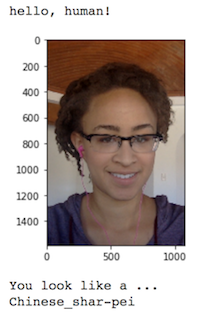
\includegraphics{images/sample_human_output.png}
\caption{Sample Human Output}
\end{figure}

\subsubsection{(IMPLEMENTATION) Write your
Algorithm}\label{implementation-write-your-algorithm}

    \begin{Verbatim}[commandchars=\\\{\}]
{\color{incolor}In [{\color{incolor}66}]:} \PY{c+c1}{\PYZsh{}\PYZsh{}\PYZsh{} TODO: Write your algorithm.}
         \PY{c+c1}{\PYZsh{}\PYZsh{}\PYZsh{} Feel free to use as many code cells as needed.}
         \PY{k+kn}{import} \PY{n+nn}{matplotlib}\PY{n+nn}{.}\PY{n+nn}{pyplot} \PY{k}{as} \PY{n+nn}{plt}
         \PY{k+kn}{import} \PY{n+nn}{matplotlib}\PY{n+nn}{.}\PY{n+nn}{image} \PY{k}{as} \PY{n+nn}{mpimg}
         \PY{k}{def} \PY{n+nf}{predict\PYZus{}breed}\PY{p}{(}\PY{n}{img\PYZus{}path}\PY{p}{)}\PY{p}{:}
             \PY{n}{is\PYZus{}human} \PY{o}{=} \PY{n}{face\PYZus{}detector}\PY{p}{(}\PY{n}{img\PYZus{}path}\PY{p}{)}
             \PY{n}{is\PYZus{}dog} \PY{o}{=} \PY{n}{dog\PYZus{}detector}\PY{p}{(}\PY{n}{img\PYZus{}path}\PY{p}{)}
             \PY{k}{if} \PY{o+ow}{not} \PY{n}{is\PYZus{}dog}\PY{p}{:}
                 \PY{k}{if} \PY{o+ow}{not} \PY{n}{is\PYZus{}human}\PY{p}{:}
                     \PY{n+nb}{print}\PY{p}{(}\PY{l+s+s2}{\PYZdq{}}\PY{l+s+s2}{Error! The algorithm cannot detect nor a human nor a dog in the picture: }\PY{l+s+si}{\PYZpc{}s}\PY{l+s+s2}{\PYZdq{}} \PY{o}{\PYZpc{}}\PY{k}{img\PYZus{}path})
                     \PY{n}{img}\PY{o}{=}\PY{n}{mpimg}\PY{o}{.}\PY{n}{imread}\PY{p}{(}\PY{n}{img\PYZus{}path}\PY{p}{)}
                     \PY{n}{plt}\PY{o}{.}\PY{n}{imshow}\PY{p}{(}\PY{n}{img}\PY{p}{)}
                     \PY{n}{plt}\PY{o}{.}\PY{n}{show}\PY{p}{(}\PY{p}{)}
                     \PY{k}{return}
                 \PY{k}{else}\PY{p}{:}
                     \PY{n+nb}{print}\PY{p}{(}\PY{l+s+s2}{\PYZdq{}}\PY{l+s+s2}{Hello, Human!}\PY{l+s+s2}{\PYZdq{}}\PY{p}{)}
             \PY{k}{else}\PY{p}{:}
                 \PY{n+nb}{print}\PY{p}{(}\PY{l+s+s2}{\PYZdq{}}\PY{l+s+s2}{Hello, Dog!}\PY{l+s+s2}{\PYZdq{}}\PY{p}{)}
             \PY{n}{img}\PY{o}{=}\PY{n}{mpimg}\PY{o}{.}\PY{n}{imread}\PY{p}{(}\PY{n}{img\PYZus{}path}\PY{p}{)}
             \PY{n}{plt}\PY{o}{.}\PY{n}{imshow}\PY{p}{(}\PY{n}{img}\PY{p}{)}
             \PY{n}{plt}\PY{o}{.}\PY{n}{show}\PY{p}{(}\PY{p}{)}
             \PY{n}{breed} \PY{o}{=} \PY{n}{get\PYZus{}predicted\PYZus{}breed}\PY{p}{(}\PY{n}{img\PYZus{}path}\PY{p}{)}
             \PY{n+nb}{print}\PY{p}{(}\PY{l+s+s2}{\PYZdq{}}\PY{l+s+s2}{You look like a }\PY{l+s+si}{\PYZpc{}s}\PY{l+s+s2}{\PYZdq{}} \PY{o}{\PYZpc{}}\PY{k}{breed})
             \PY{k}{return}
             
             
\end{Verbatim}


    \begin{center}\rule{0.5\linewidth}{\linethickness}\end{center}

 \#\# Step 7: Test Your Algorithm

In this section, you will take your new algorithm for a spin! What kind
of dog does the algorithm think that \textbf{you} look like? If you have
a dog, does it predict your dog's breed accurately? If you have a cat,
does it mistakenly think that your cat is a dog?

\subsubsection{(IMPLEMENTATION) Test Your Algorithm on Sample
Images!}\label{implementation-test-your-algorithm-on-sample-images}

Test your algorithm at least six images on your computer. Feel free to
use any images you like. Use at least two human and two dog images.

\textbf{Question 6:} Is the output better than you expected :) ? Or
worse :( ? Provide at least three possible points of improvement for
your algorithm.

\textbf{Answer:} It correctly classified the breed of the test images,
and correctly recognized the humans. But the painting from a turkey it
uncorrectly classified as a Human. For the dogs it's better, then I
expected, but for human recognition it worse.

Improvement possiblities: - add more convulational layer after ResNet50
- add a CNN for human recognition - add augmented images for the
training dataset

    \begin{Verbatim}[commandchars=\\\{\}]
{\color{incolor}In [{\color{incolor}69}]:} \PY{c+c1}{\PYZsh{}\PYZsh{} TODO: Execute your algorithm from Step 6 on}
         \PY{c+c1}{\PYZsh{}\PYZsh{} at least 6 images on your computer.}
         \PY{c+c1}{\PYZsh{}\PYZsh{} Feel free to use as many code cells as needed.}
         \PY{n}{img\PYZus{}paths} \PY{o}{=} \PY{n}{np}\PY{o}{.}\PY{n}{array}\PY{p}{(}\PY{n}{glob}\PY{p}{(}\PY{l+s+s2}{\PYZdq{}}\PY{l+s+s2}{test\PYZus{}images/*}\PY{l+s+s2}{\PYZdq{}}\PY{p}{)}\PY{p}{)}
         \PY{k}{for} \PY{n}{img\PYZus{}path} \PY{o+ow}{in} \PY{n}{img\PYZus{}paths}\PY{p}{:}
             \PY{n}{predict\PYZus{}breed}\PY{p}{(}\PY{n}{img\PYZus{}path}\PY{p}{)}
\end{Verbatim}


    \begin{Verbatim}[commandchars=\\\{\}]
Hello, Human!

    \end{Verbatim}

    \begin{center}
    \adjustimage{max size={0.9\linewidth}{0.9\paperheight}}{output_65_1.png}
    \end{center}
    { \hspace*{\fill} \\}
    
    \begin{Verbatim}[commandchars=\\\{\}]
You look like a Great\_dane
Hello, Dog!

    \end{Verbatim}

    \begin{center}
    \adjustimage{max size={0.9\linewidth}{0.9\paperheight}}{output_65_3.png}
    \end{center}
    { \hspace*{\fill} \\}
    
    \begin{Verbatim}[commandchars=\\\{\}]
You look like a Poodle
Hello, Human!

    \end{Verbatim}

    \begin{center}
    \adjustimage{max size={0.9\linewidth}{0.9\paperheight}}{output_65_5.png}
    \end{center}
    { \hspace*{\fill} \\}
    
    \begin{Verbatim}[commandchars=\\\{\}]
You look like a Great\_dane
Error! The algorithm cannot detect nor a human nor a dog in the picture: test\_images\textbackslash{}rabbit.jpg

    \end{Verbatim}

    \begin{center}
    \adjustimage{max size={0.9\linewidth}{0.9\paperheight}}{output_65_7.png}
    \end{center}
    { \hspace*{\fill} \\}
    
    \begin{Verbatim}[commandchars=\\\{\}]
Hello, Dog!

    \end{Verbatim}

    \begin{center}
    \adjustimage{max size={0.9\linewidth}{0.9\paperheight}}{output_65_9.png}
    \end{center}
    { \hspace*{\fill} \\}
    
    \begin{Verbatim}[commandchars=\\\{\}]
You look like a Beagle
Hello, Human!

    \end{Verbatim}

    \begin{center}
    \adjustimage{max size={0.9\linewidth}{0.9\paperheight}}{output_65_11.png}
    \end{center}
    { \hspace*{\fill} \\}
    
    \begin{Verbatim}[commandchars=\\\{\}]
You look like a English\_toy\_spaniel
Hello, Human!

    \end{Verbatim}

    \begin{center}
    \adjustimage{max size={0.9\linewidth}{0.9\paperheight}}{output_65_13.png}
    \end{center}
    { \hspace*{\fill} \\}
    
    \begin{Verbatim}[commandchars=\\\{\}]
You look like a Brussels\_griffon

    \end{Verbatim}


    % Add a bibliography block to the postdoc
    
    
    
    \end{document}
